\chapter{Results}

\label{ch:Results}

This chapter presents the results of six topology-optimized designs in a thematic comparative framework, covering target modes LG$_{\ell,0}$ for $\ell = 0$ through $\ell = 5$. Each section systematically compares all six datasets for the same physical quantity, highlighting how the topological charge affects design characteristics. Sections 4.5.3 and 4.7 are based on post-processing forward simulations re-run with the best density distribution $\bar{\rho}^{*}$ after optimization is complete ($\beta = 512$, final binarized structure); all other results display the best outcome found during optimization at the final $\beta = 512$ stage.

%===================================================================


\section{Optimization Process}

\label{sec:opt_process}

This section shows the convergence history of the six designs, including the $\beta$ schedule, FOM curves, and mode purity evolution, to verify the numerical stability of the $\beta$ continuation strategy.

\subsection{Beta Continuation Schedule and FOM Convergence}

\label{ssec:opt_FOM}

All six designs use the same $\beta$ schedule: starting from $\beta = 4$ and increasing at fixed iteration intervals to a final $\beta = 512$, with each $\beta$ switch marked by a purple vertical line (see Figure~\ref{fig:FOM_history_all}). The FOM curves for all designs show a large upward trend during the $\beta < 16$ stage, reaching their highest values near the end of this interval. This convergence pattern reflects the fact that the looser boundary conditions at low $\beta$ allow the optimizer to explore the continuous density space freely and efficiently find globally better topological layouts that achieve peak performance.

The final FOM values for low topological charges $\ell = 0, 1$ ($0.39$ and higher) are noticeably higher than for high topological charges $\ell = 3, 4, 5$ (FOM $\approx 0.30$ to $0.19$), indicating that higher-order OAM modes require more complex phase modulation, which limits the final coupling efficiency. Notably, although the FOM value for $\ell = 3$ is slightly lower, performance recovers very quickly after each $\beta$ switch, showing that increasing the topological charge does not significantly worsen the convergence behavior.

\begin{figure}[htb]
\centering
	\begin{tabular}{cc} 
	    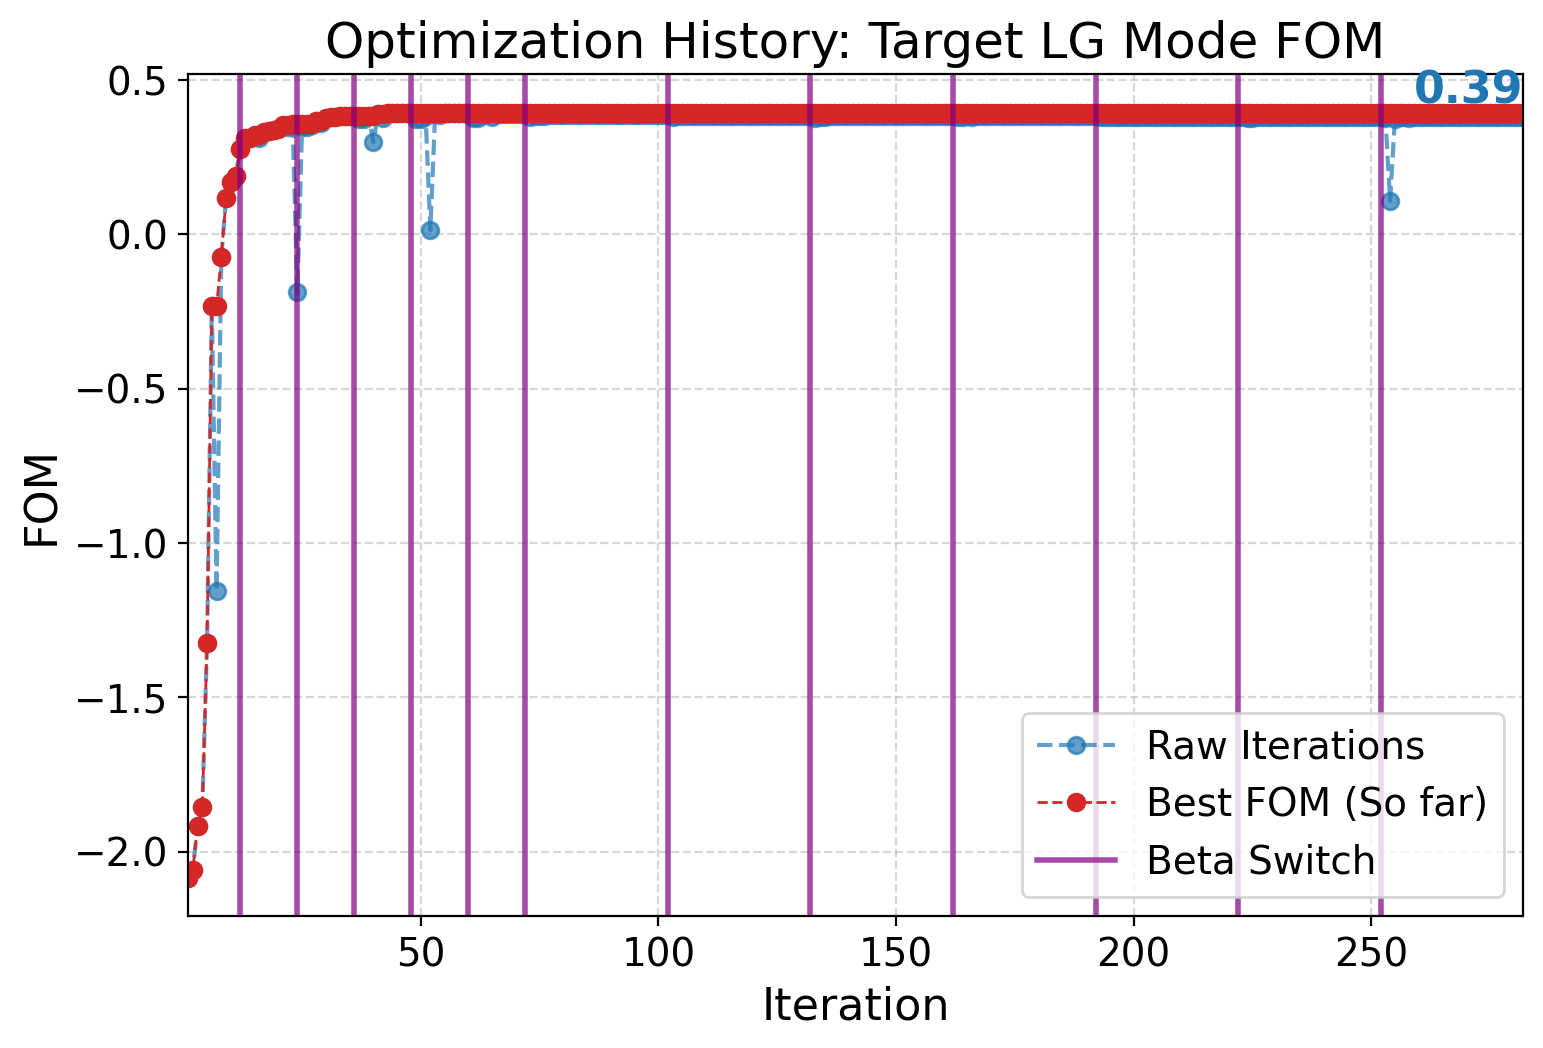
\includegraphics[width=0.47\textwidth]{img/017_FOM_history_staircase.png} &
	    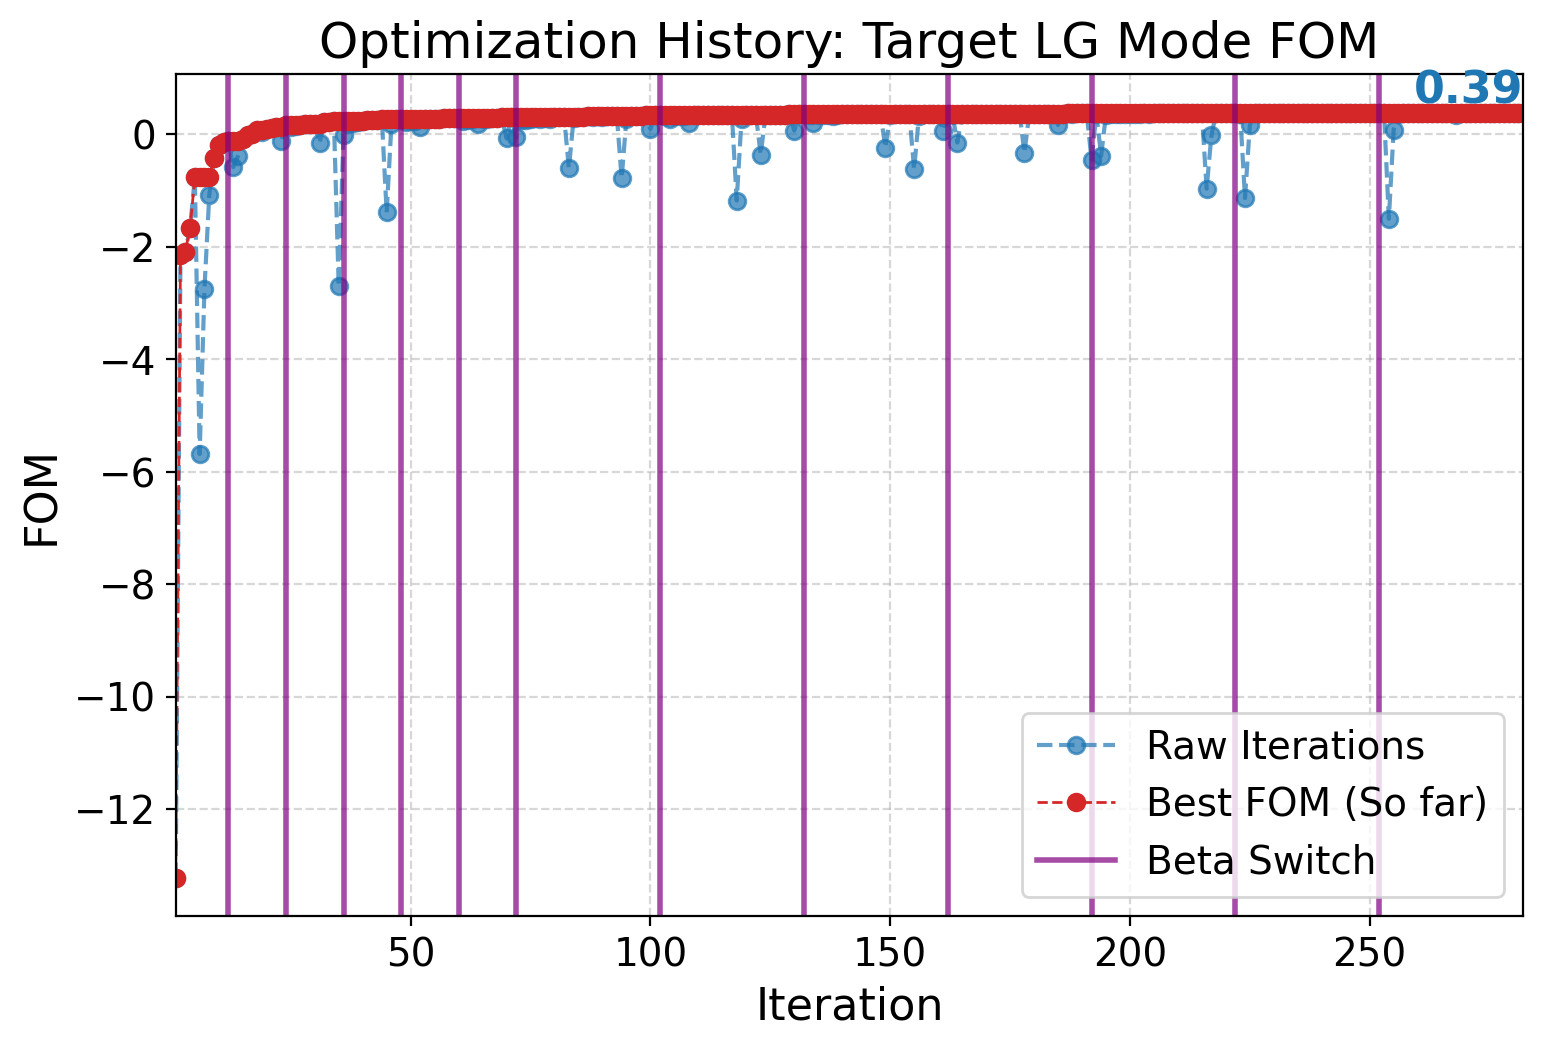
\includegraphics[width=0.47\textwidth]{img/018_FOM_history_staircase.png}
		\\ (a) & (b) \\[6pt]
		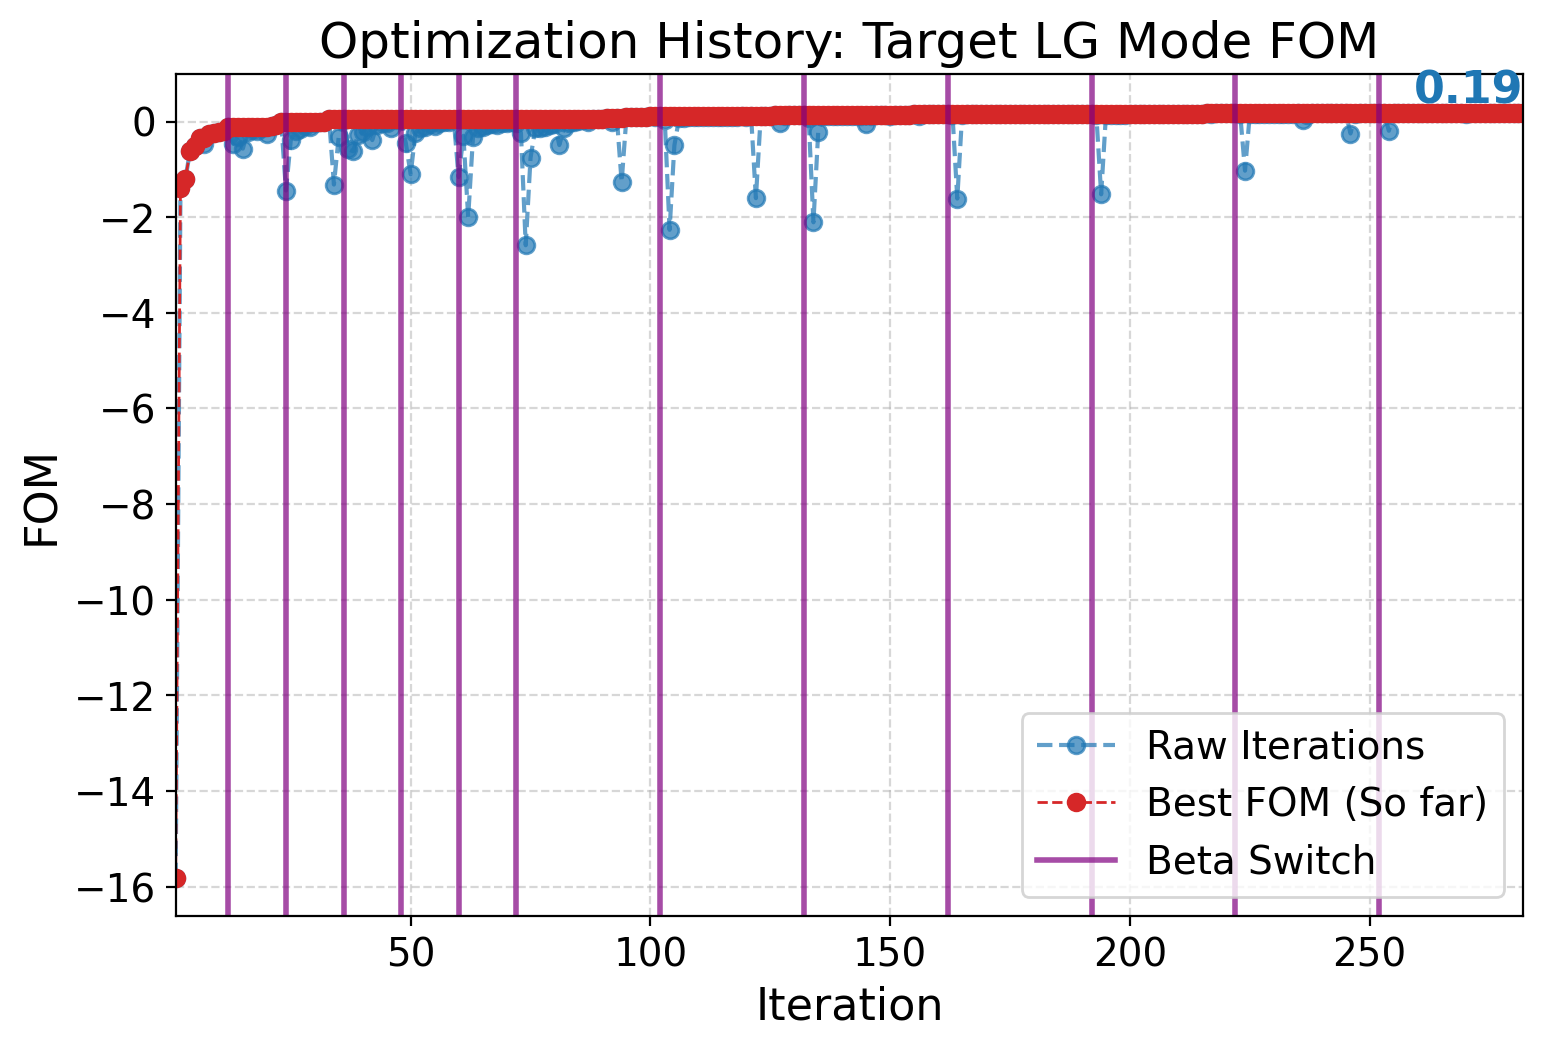
\includegraphics[width=0.47\textwidth]{img/013_FOM_history_staircase.png}&
		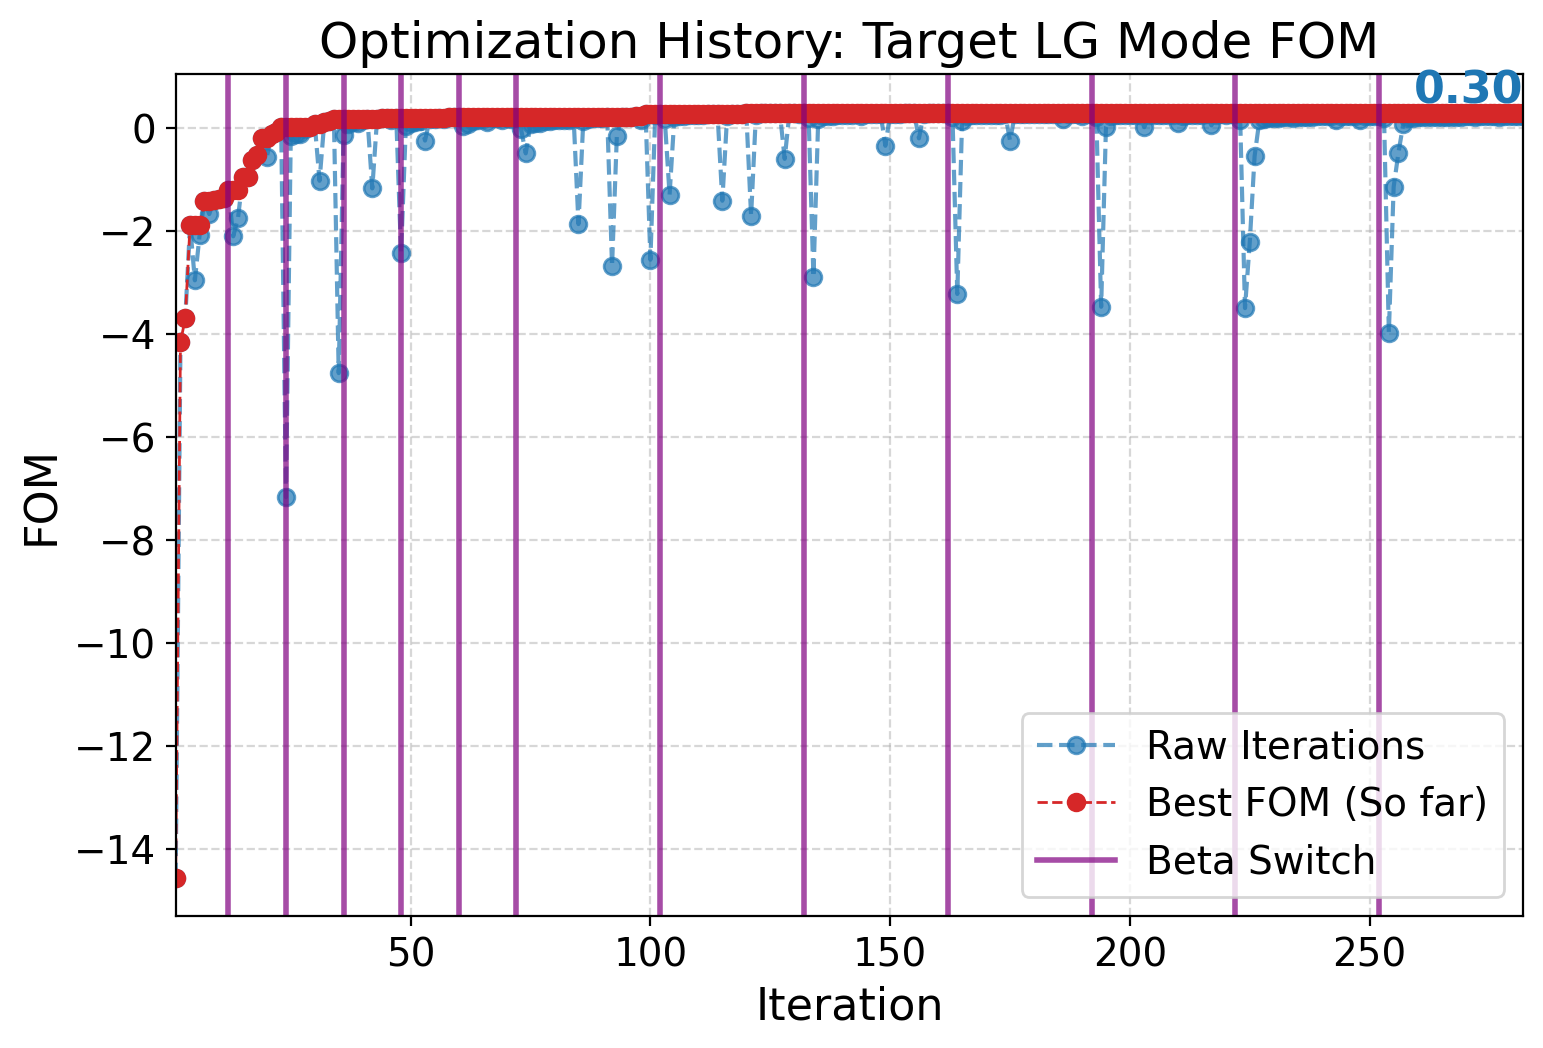
\includegraphics[width=0.47\textwidth]{img/020_FOM_history_staircase.png}
	    \\  (c)  & (d) \\[6pt]
	    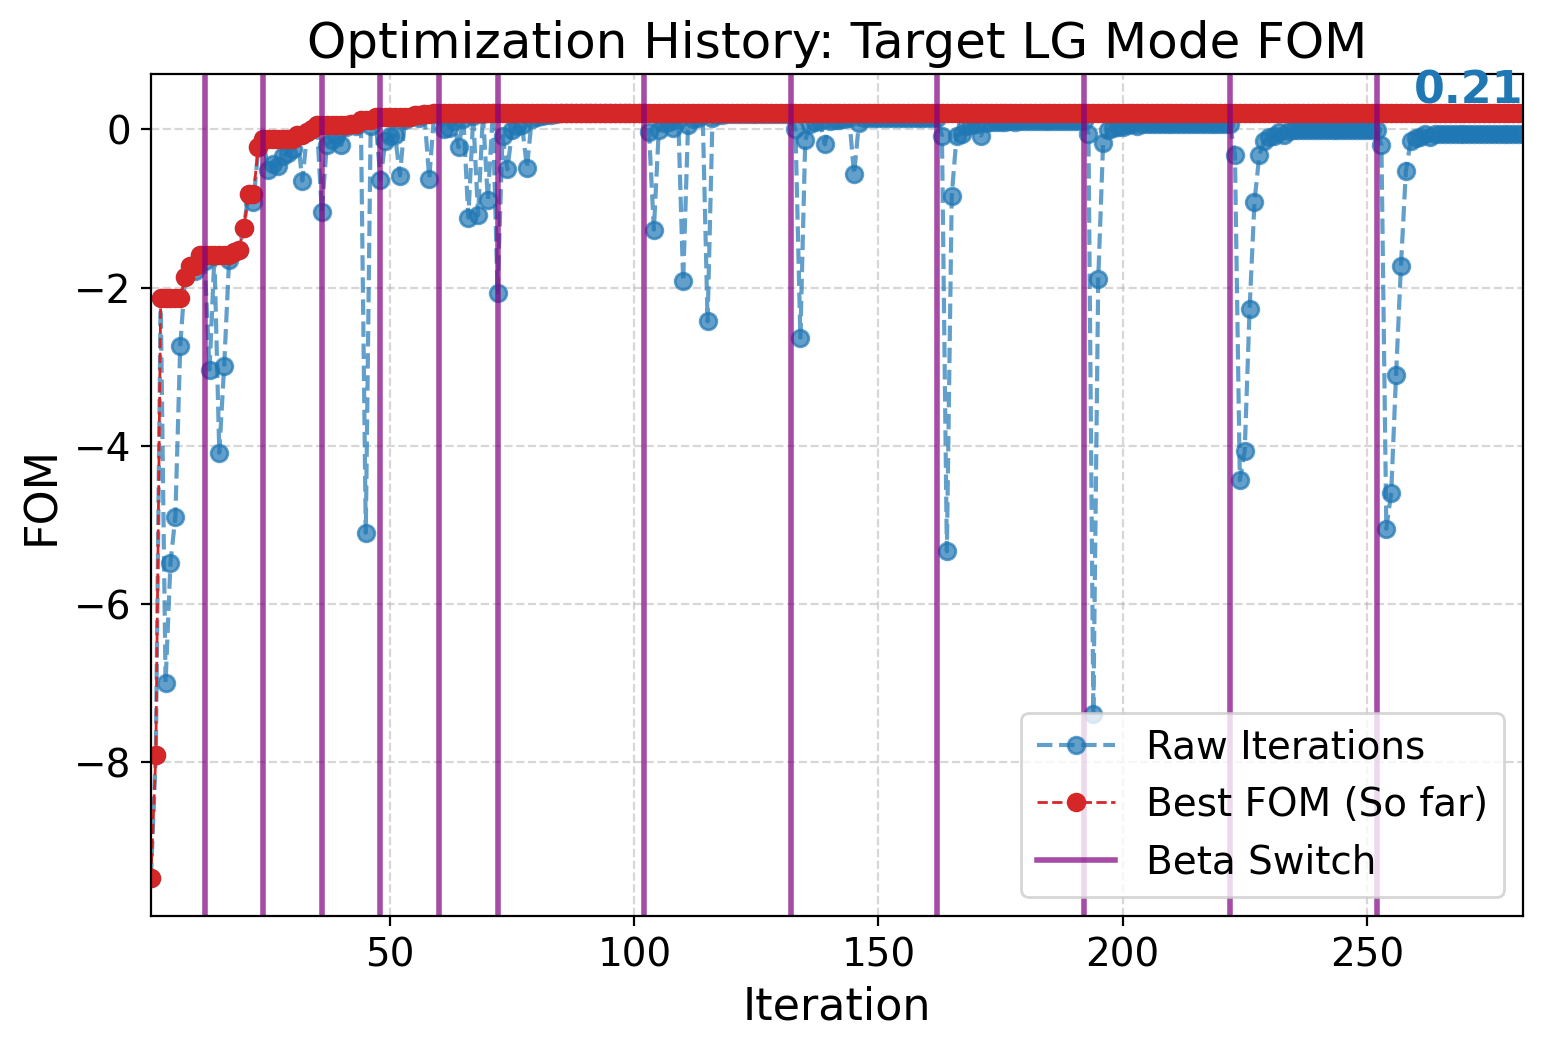
\includegraphics[width=0.47\textwidth]{img/021_FOM_history_staircase.png}&
	    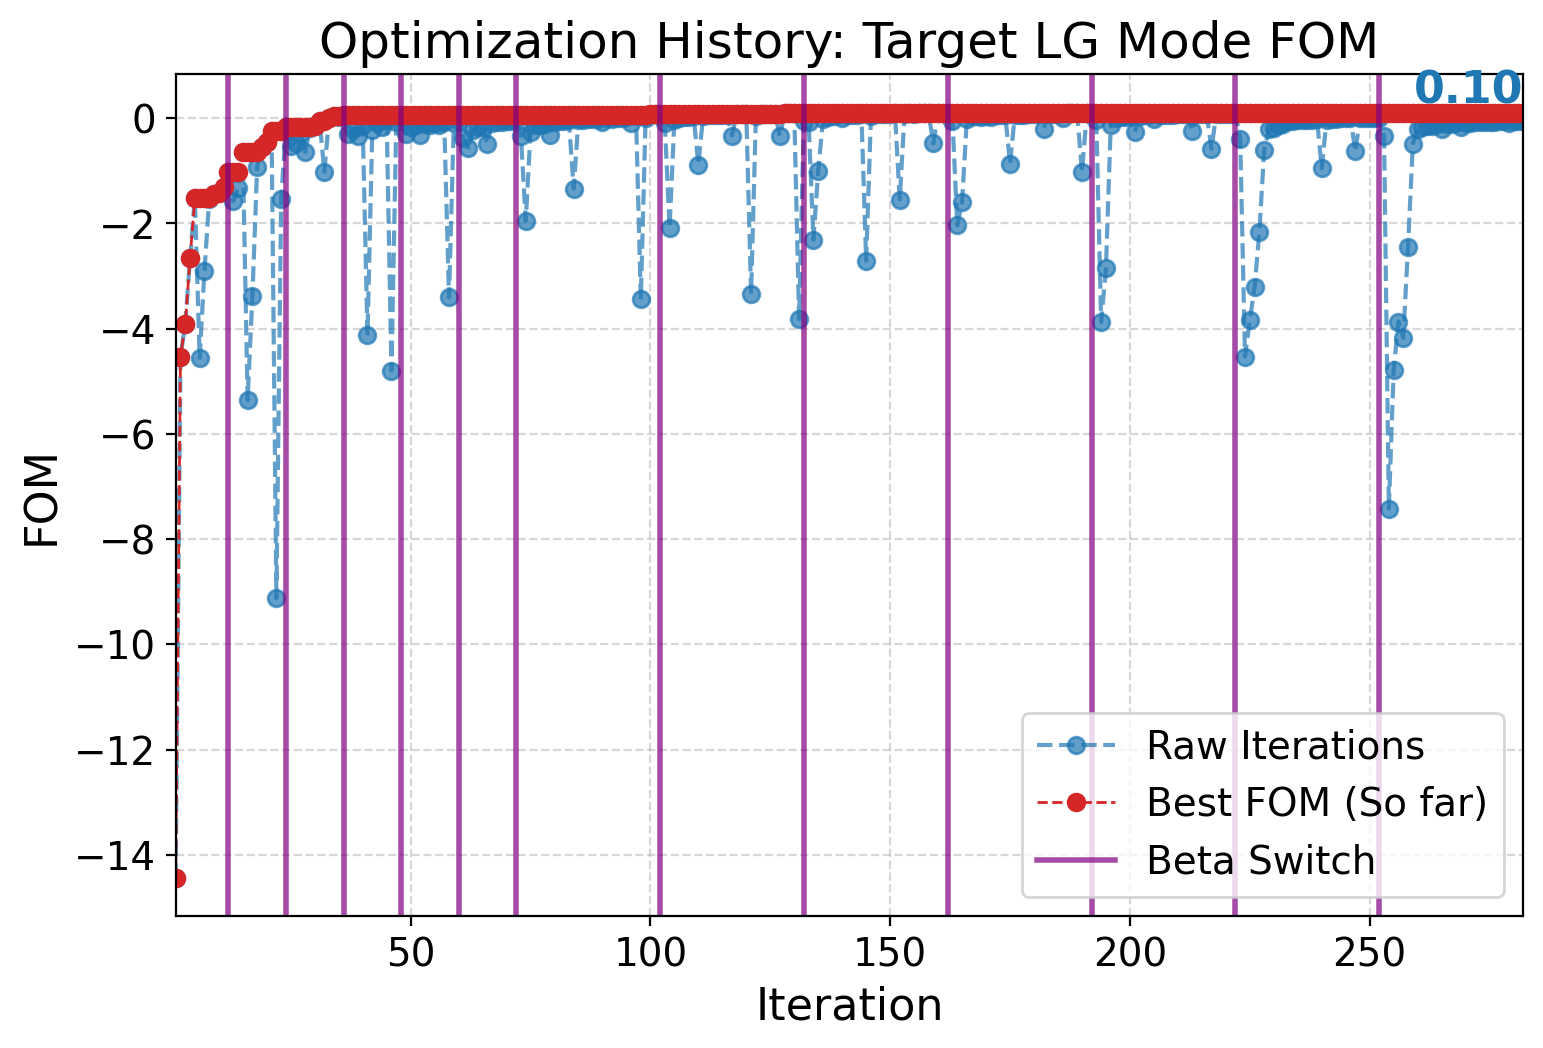
\includegraphics[width=0.47\textwidth]{img/022_FOM_history_staircase.png}
	    \\ (e) & (f)
	\end{tabular}
\caption{FOM convergence history: (a)$\sim$(f) $\ell \in \{0, 1, 2, 3, 4, 5\}$, respectively. Blue dashed line: raw FOM value at each iteration; red dashed line: best-so-far tracking value; purple vertical lines: $\beta$ continuation switch points ($\beta_\text{final} = 512$).}
\label{fig:FOM_history_all}
\end{figure}




\subsection{Mode Purity Convergence}

\label{ssec:opt_purity}

Figure~\ref{fig:purity_history_all} shows the mode purity convergence history for the six designs. The purity evolution closely tracks the FOM history: the main structure forms rapidly in the early stage, and purity saturates and stabilizes after the 2nd to 4th $\beta$ switches.

Low topological charge designs $\ell = 0, 1, 2$ all achieve final purity above $96\%$, with $\ell = 1$ reaching the highest of all six at $98.66\%$, indicating the best solution quality under these design conditions. As topological charge increases, $\ell = 3$ drops to $94.13\%$, while $\ell = 4$ and $\ell = 5$ fall further to $81.94\%$ and $82.62\%$. In the high topological charge cases, the finite $4.5\;\mu\text{m}$ design area size and resolution limit mean the high-order OAM modes are approaching their physical limits. Purity therefore hits a ceiling early in the optimization, and further increases in $\beta$ only cause structural boundary oscillations without improving the final purity.

The final quantitative results for $\ell = 0$ to $5$ are summarized in Table~\ref{tab:results_summary}.

\begin{figure}[htb]
\centering
	\begin{tabular}{cc} 
	    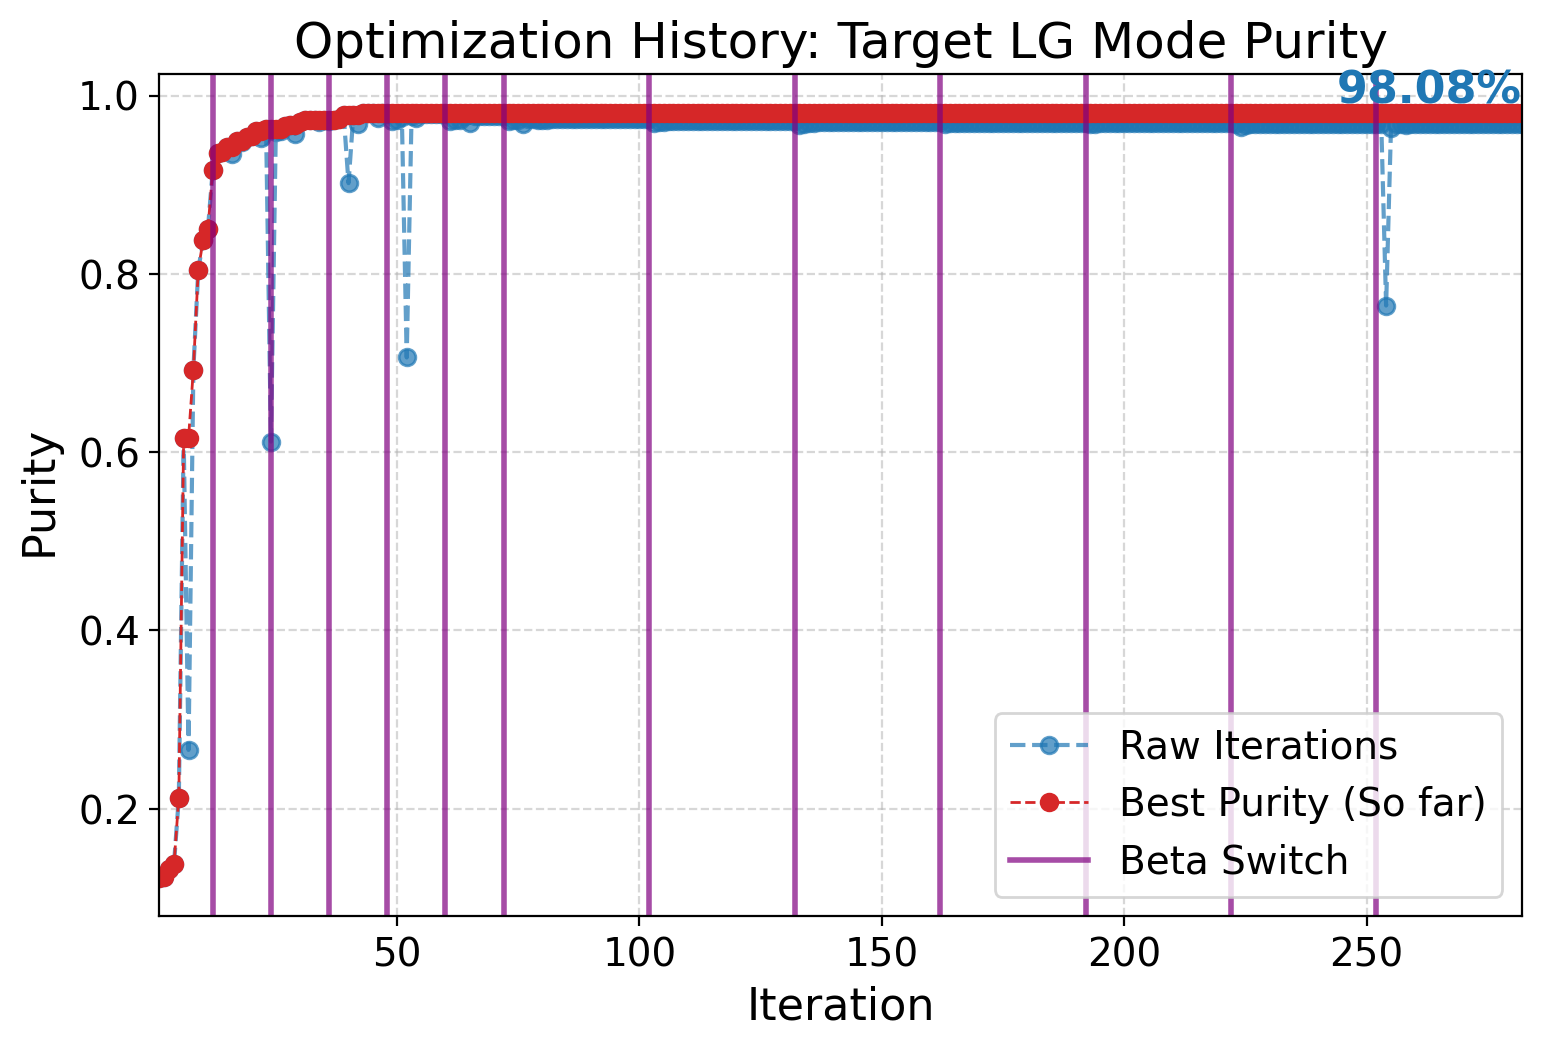
\includegraphics[width=0.47\textwidth]{img/017_purity_history_staircase.png}&
	    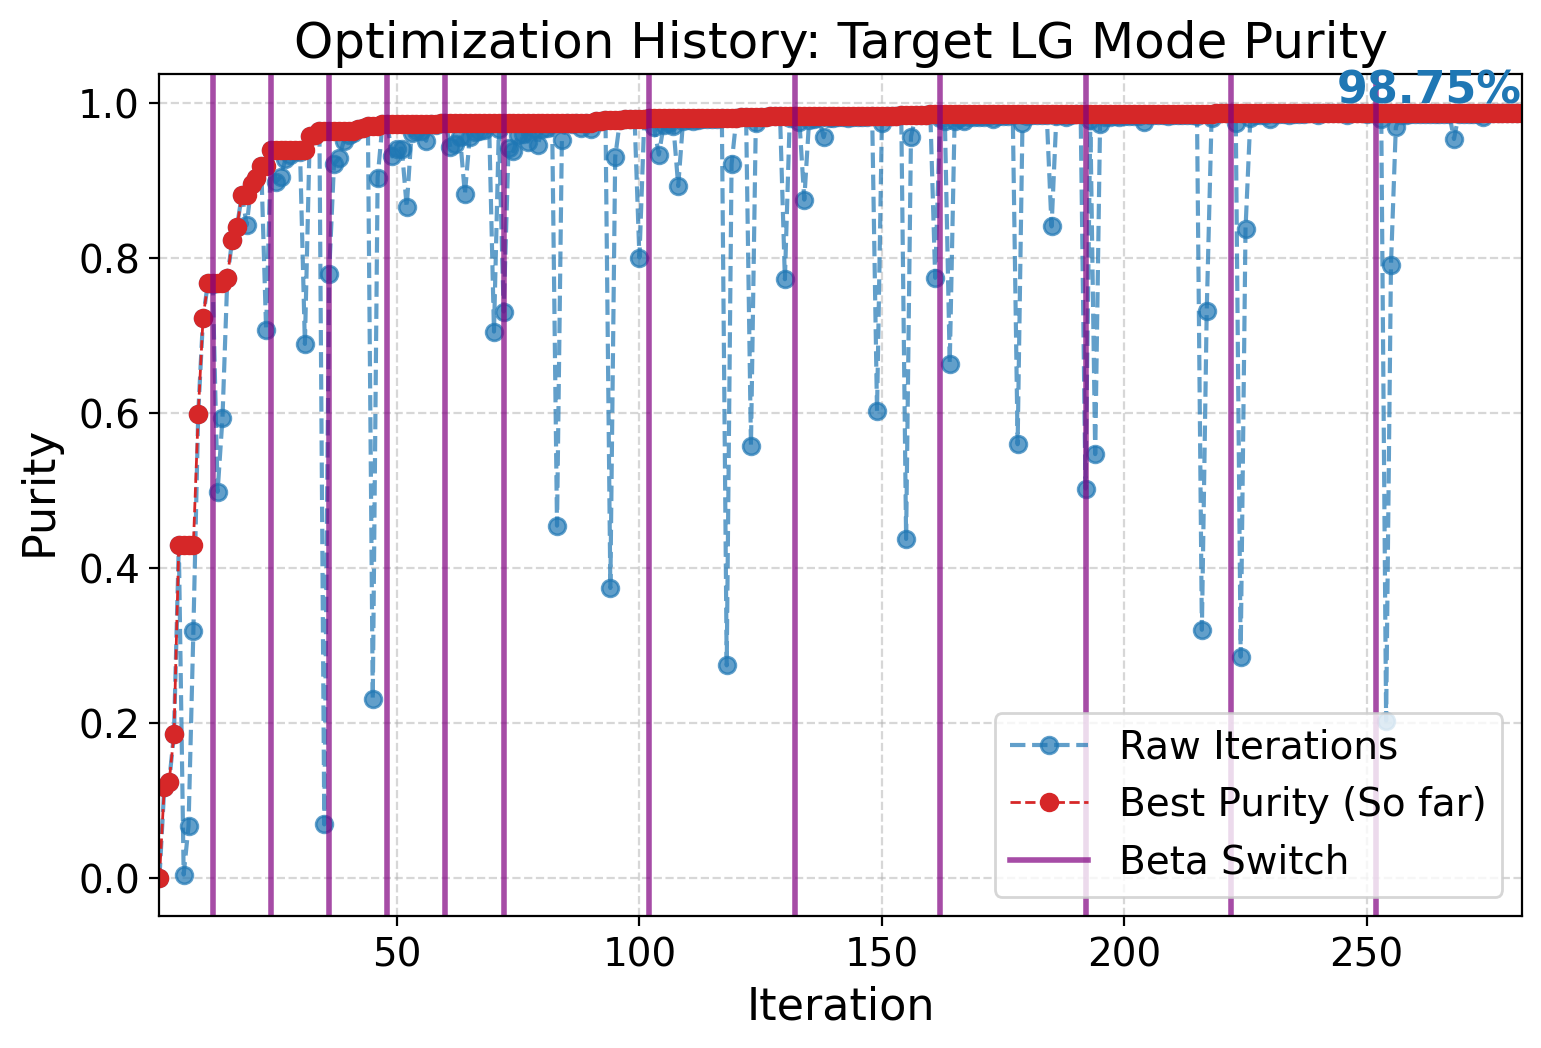
\includegraphics[width=0.47\textwidth]{img/018_purity_history_staircase.png}
		\\ (a) & (b) \\[6pt]
		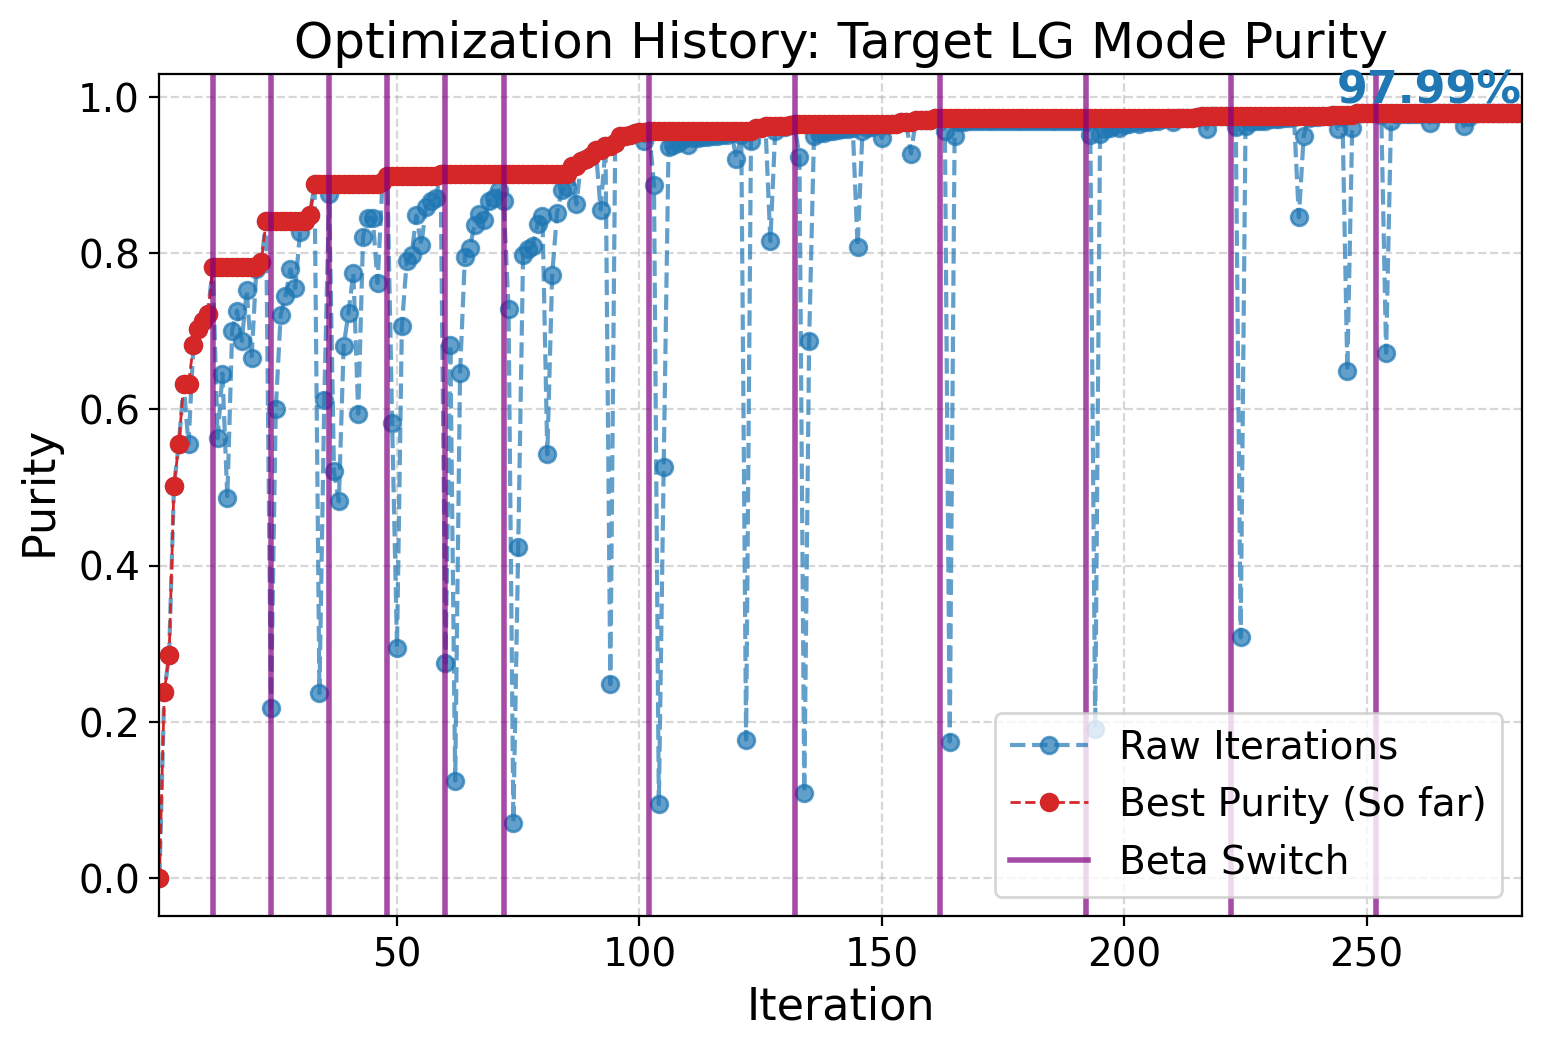
\includegraphics[width=0.47\textwidth]{img/013_purity_history_staircase.png}&
	    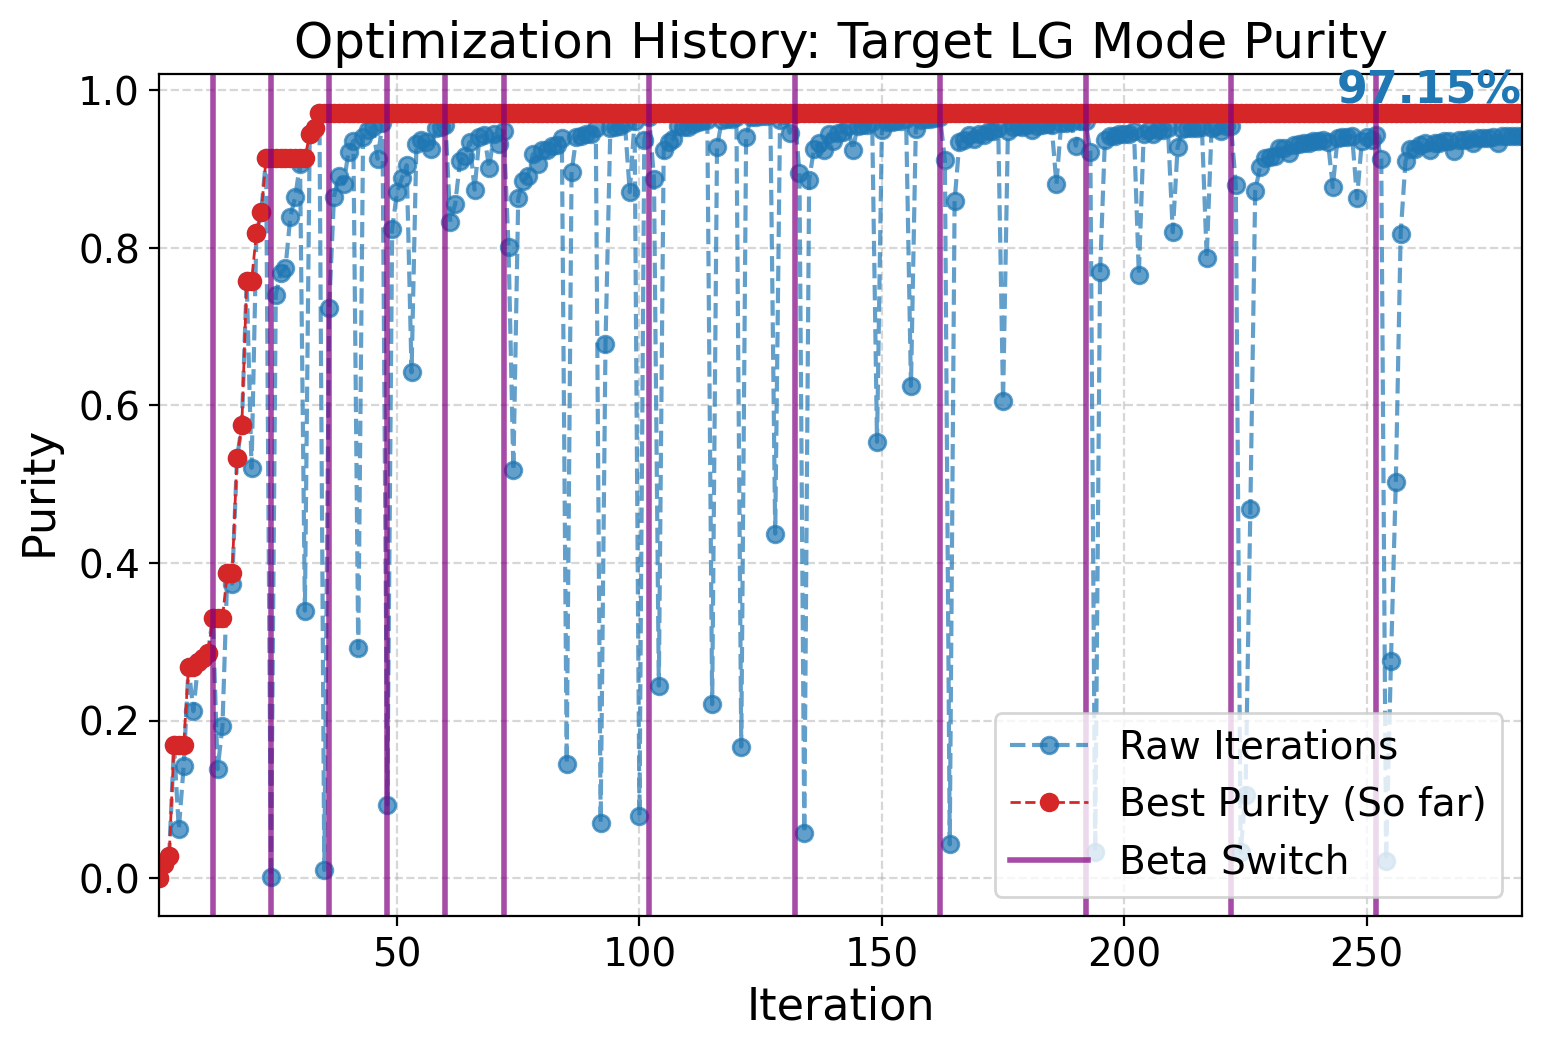
\includegraphics[width=0.47\textwidth]{img/020_purity_history_staircase.png}
	    \\  (c) & (d)\\[6pt]
	    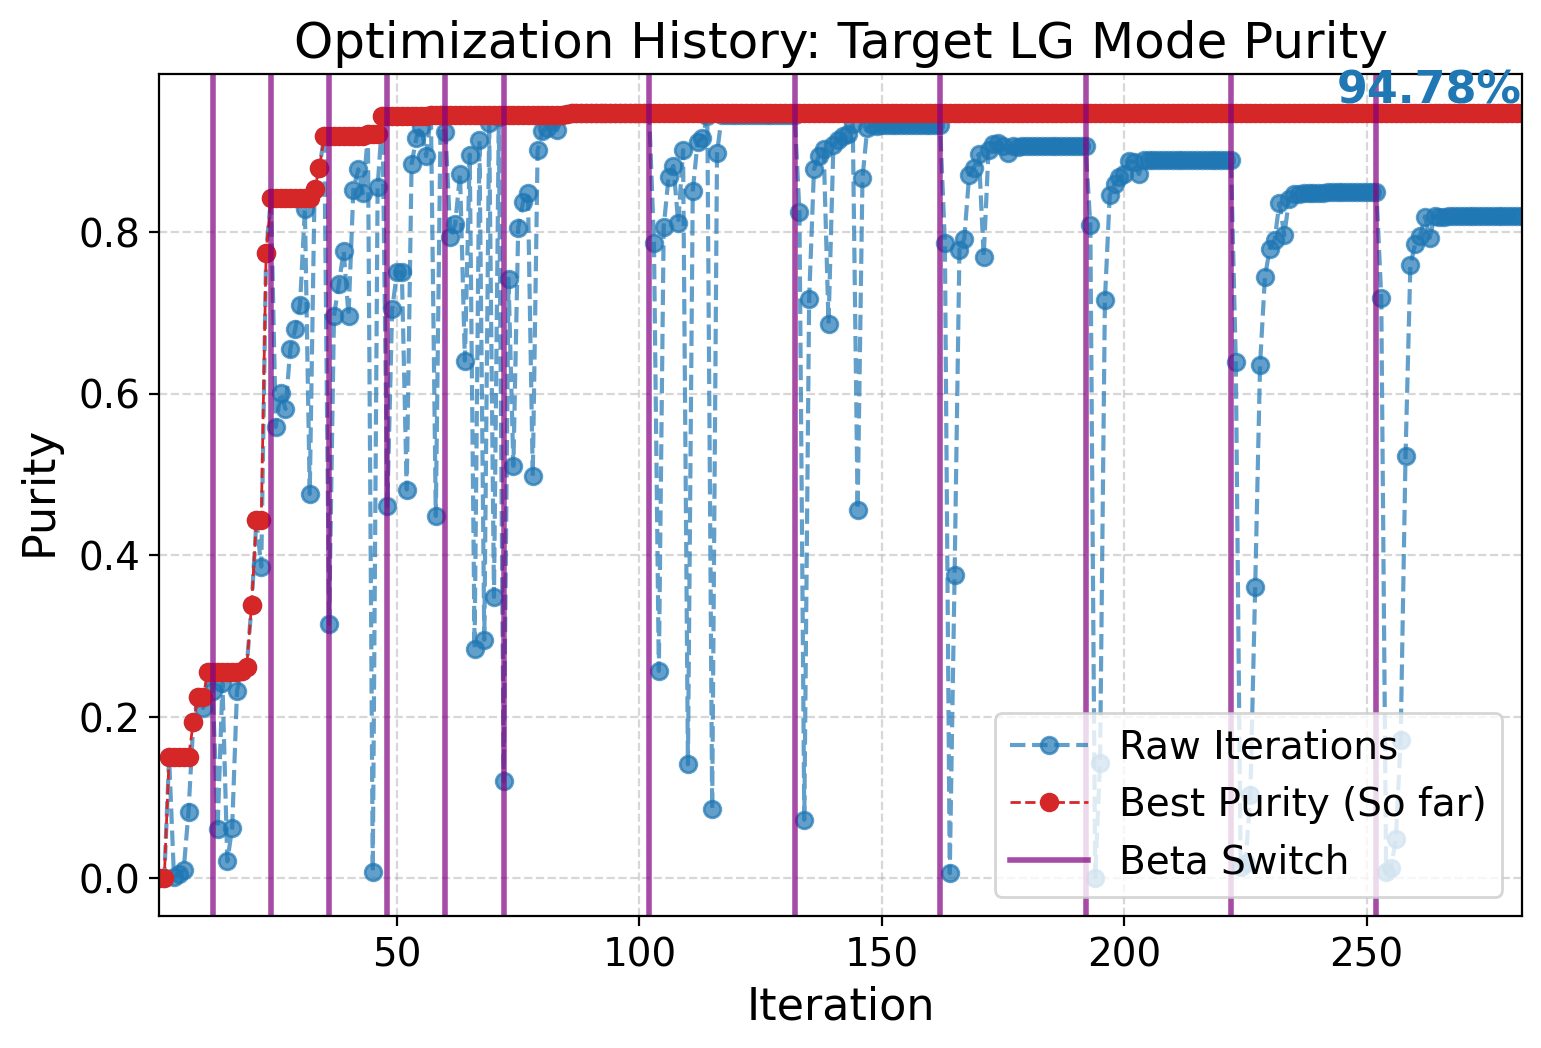
\includegraphics[width=0.47\textwidth]{img/021_purity_history_staircase.png}&
	    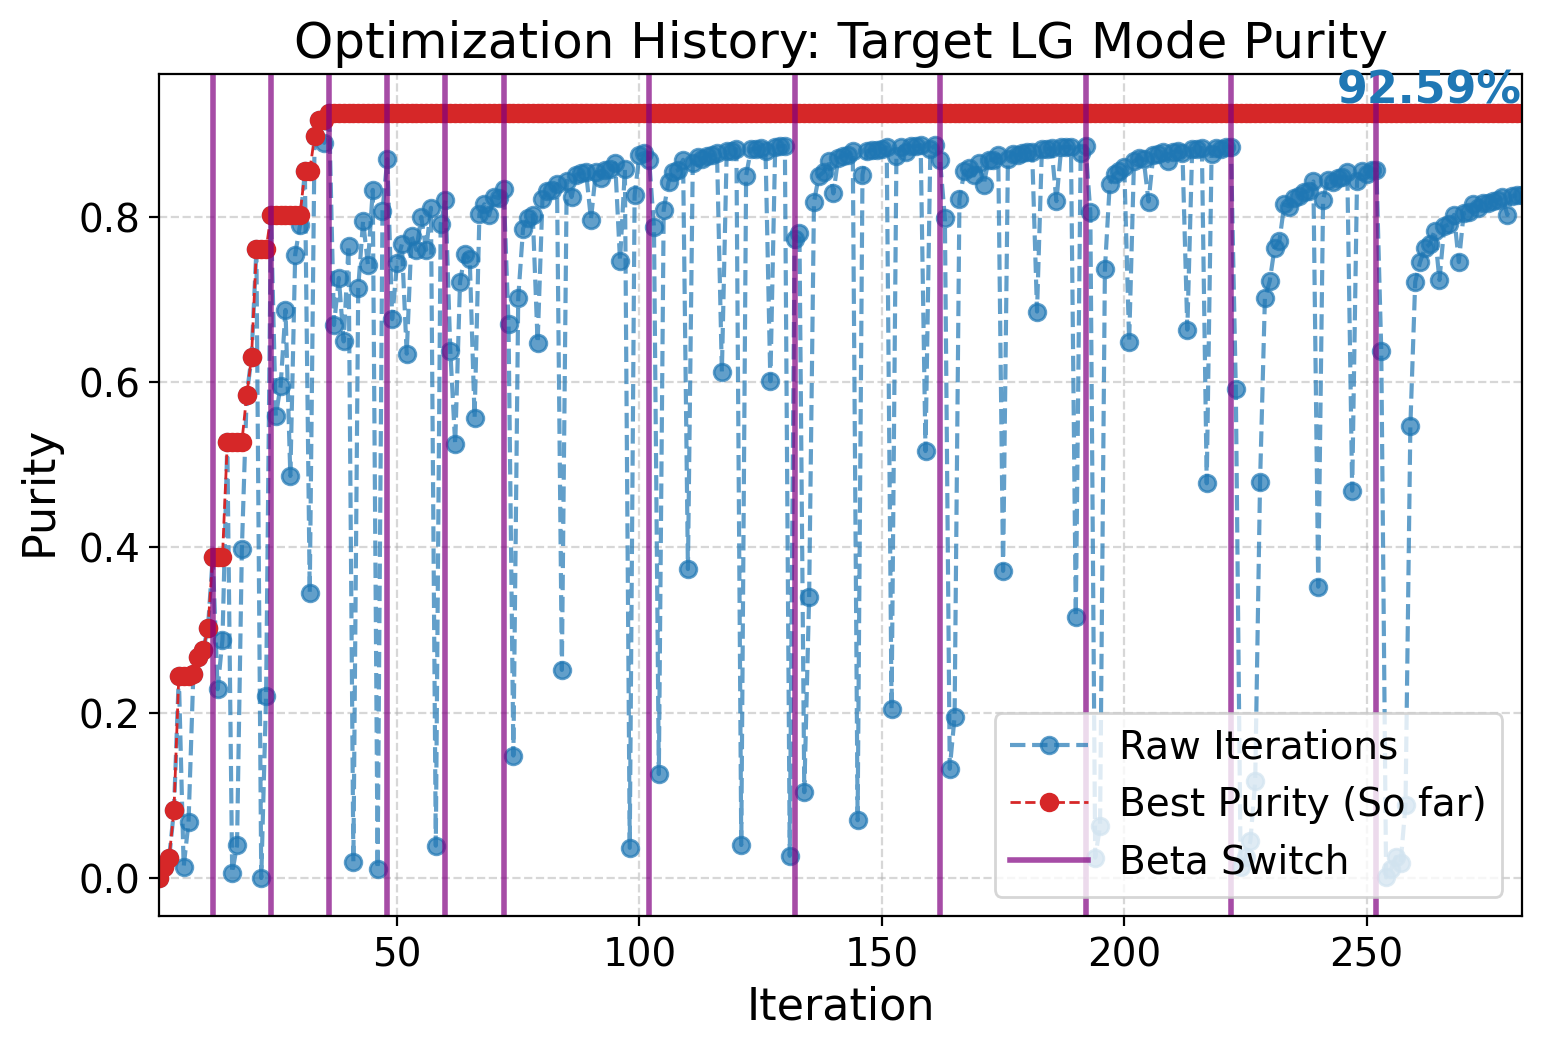
\includegraphics[width=0.47\textwidth]{img/022_purity_history_staircase.png}
	    \\ (e) & (f) 
	\end{tabular}
\caption{Mode purity convergence history: (a)$\sim$(f) $\ell \in \{0, 1, 2, 3, 4, 5\}$, respectively. Blue dashed line: instantaneous value at each iteration; red dashed line: best-so-far tracking value; purple vertical lines: $\beta$ switch points. The final best purity value is indicated in the upper right corner.}
\label{fig:purity_history_all}
\end{figure}



\begin{table}[htb]
\centering
\caption{Performance summary for $\ell = 0$ to $5$ (far-field plane at $z = 10\,z_R$).}
\label{tab:results_summary}
    \begin{tabular}{ccccc}
        \hline
        $\ell$ & Target mode & Purity (\%) & $|\text{Overlap}|^{2}$ & FOM\\
        \hline
        0 & LG$_{0,0}$ & 96.81 & 60.92 & 0.38\\
        1 & LG$_{1,0}$ & 98.66 & 53.88 &  0.39\\
        2 & LG$_{2,0}$ & 97.96 & 7.99 & 0.19\\
        3 & LG$_{3,0}$ & 94.13 & 18.69 & 0.23\\
        4 & LG$_{4,0}$ & 81.94 & 4.00 & -0.06 \\
        5 & LG$_{5,0}$ & 82.62 & 3.96 & -0.05\\
        \hline
    \end{tabular}
\end{table}

%===================================================================

\section{Optimized Structures}

\label{sec:structures}


Figure~\ref{fig:structures_all} shows the final converged GaP/air binary material density distributions for the six designs (black represents GaP, refractive index $n = 3.31$; white represents air, refractive index $n = 1$).

Examining the six structures, the most visually striking feature appears in the $\ell = 2$ design (Figure~\ref{fig:structures_all}(c)): a clear two-arm spiral pattern is visible at the center, closely resembling the working principle of a spiral phase plate (SPP). This suggests that the optimizer, guided by adjoint gradients, spontaneously discovers a design strategy similar to a two-arm SPP to provide the required $2 \times 2\pi$ azimuthal phase modulation. The surrounding scattering features act as a compensation mechanism to correct near-field coupling errors and improve far-field mode shaping accuracy.

For the other designs, the structures do not show simple $\ell$-fold rotational spiral features. $\ell = 0$ shows a roughly symmetric closed GaP core at the center; $\ell = 1, 3, 4, 5$ produce free-form, non-intuitive material distributions with no obvious geometric regularity. This reflects the nature of topology optimization: when the SPP-like spiral strategy is not the globally optimal solution, the optimizer automatically searches for an alternative distribution that better satisfies the gradient conditions, even if the result has no geometric symmetry that is easy to interpret visually.

The exclusive appearance of the $\ell$-fold spiral structure in the $\ell = 2$ design, and its absence in all other designs, can be understood through a discrete rotational symmetry selection rule discussed in Section~\ref{ssec:spiral_emergence}.

Despite the different geometric forms, all six structures show dense scattering features away from the center. As topological charge increases, these surrounding features become denser, reflecting the higher modulation demand on azimuthal phase space for higher-order OAM modes.


\begin{figure}[htb]
\centering
    \begin{tabular}{ccc}
        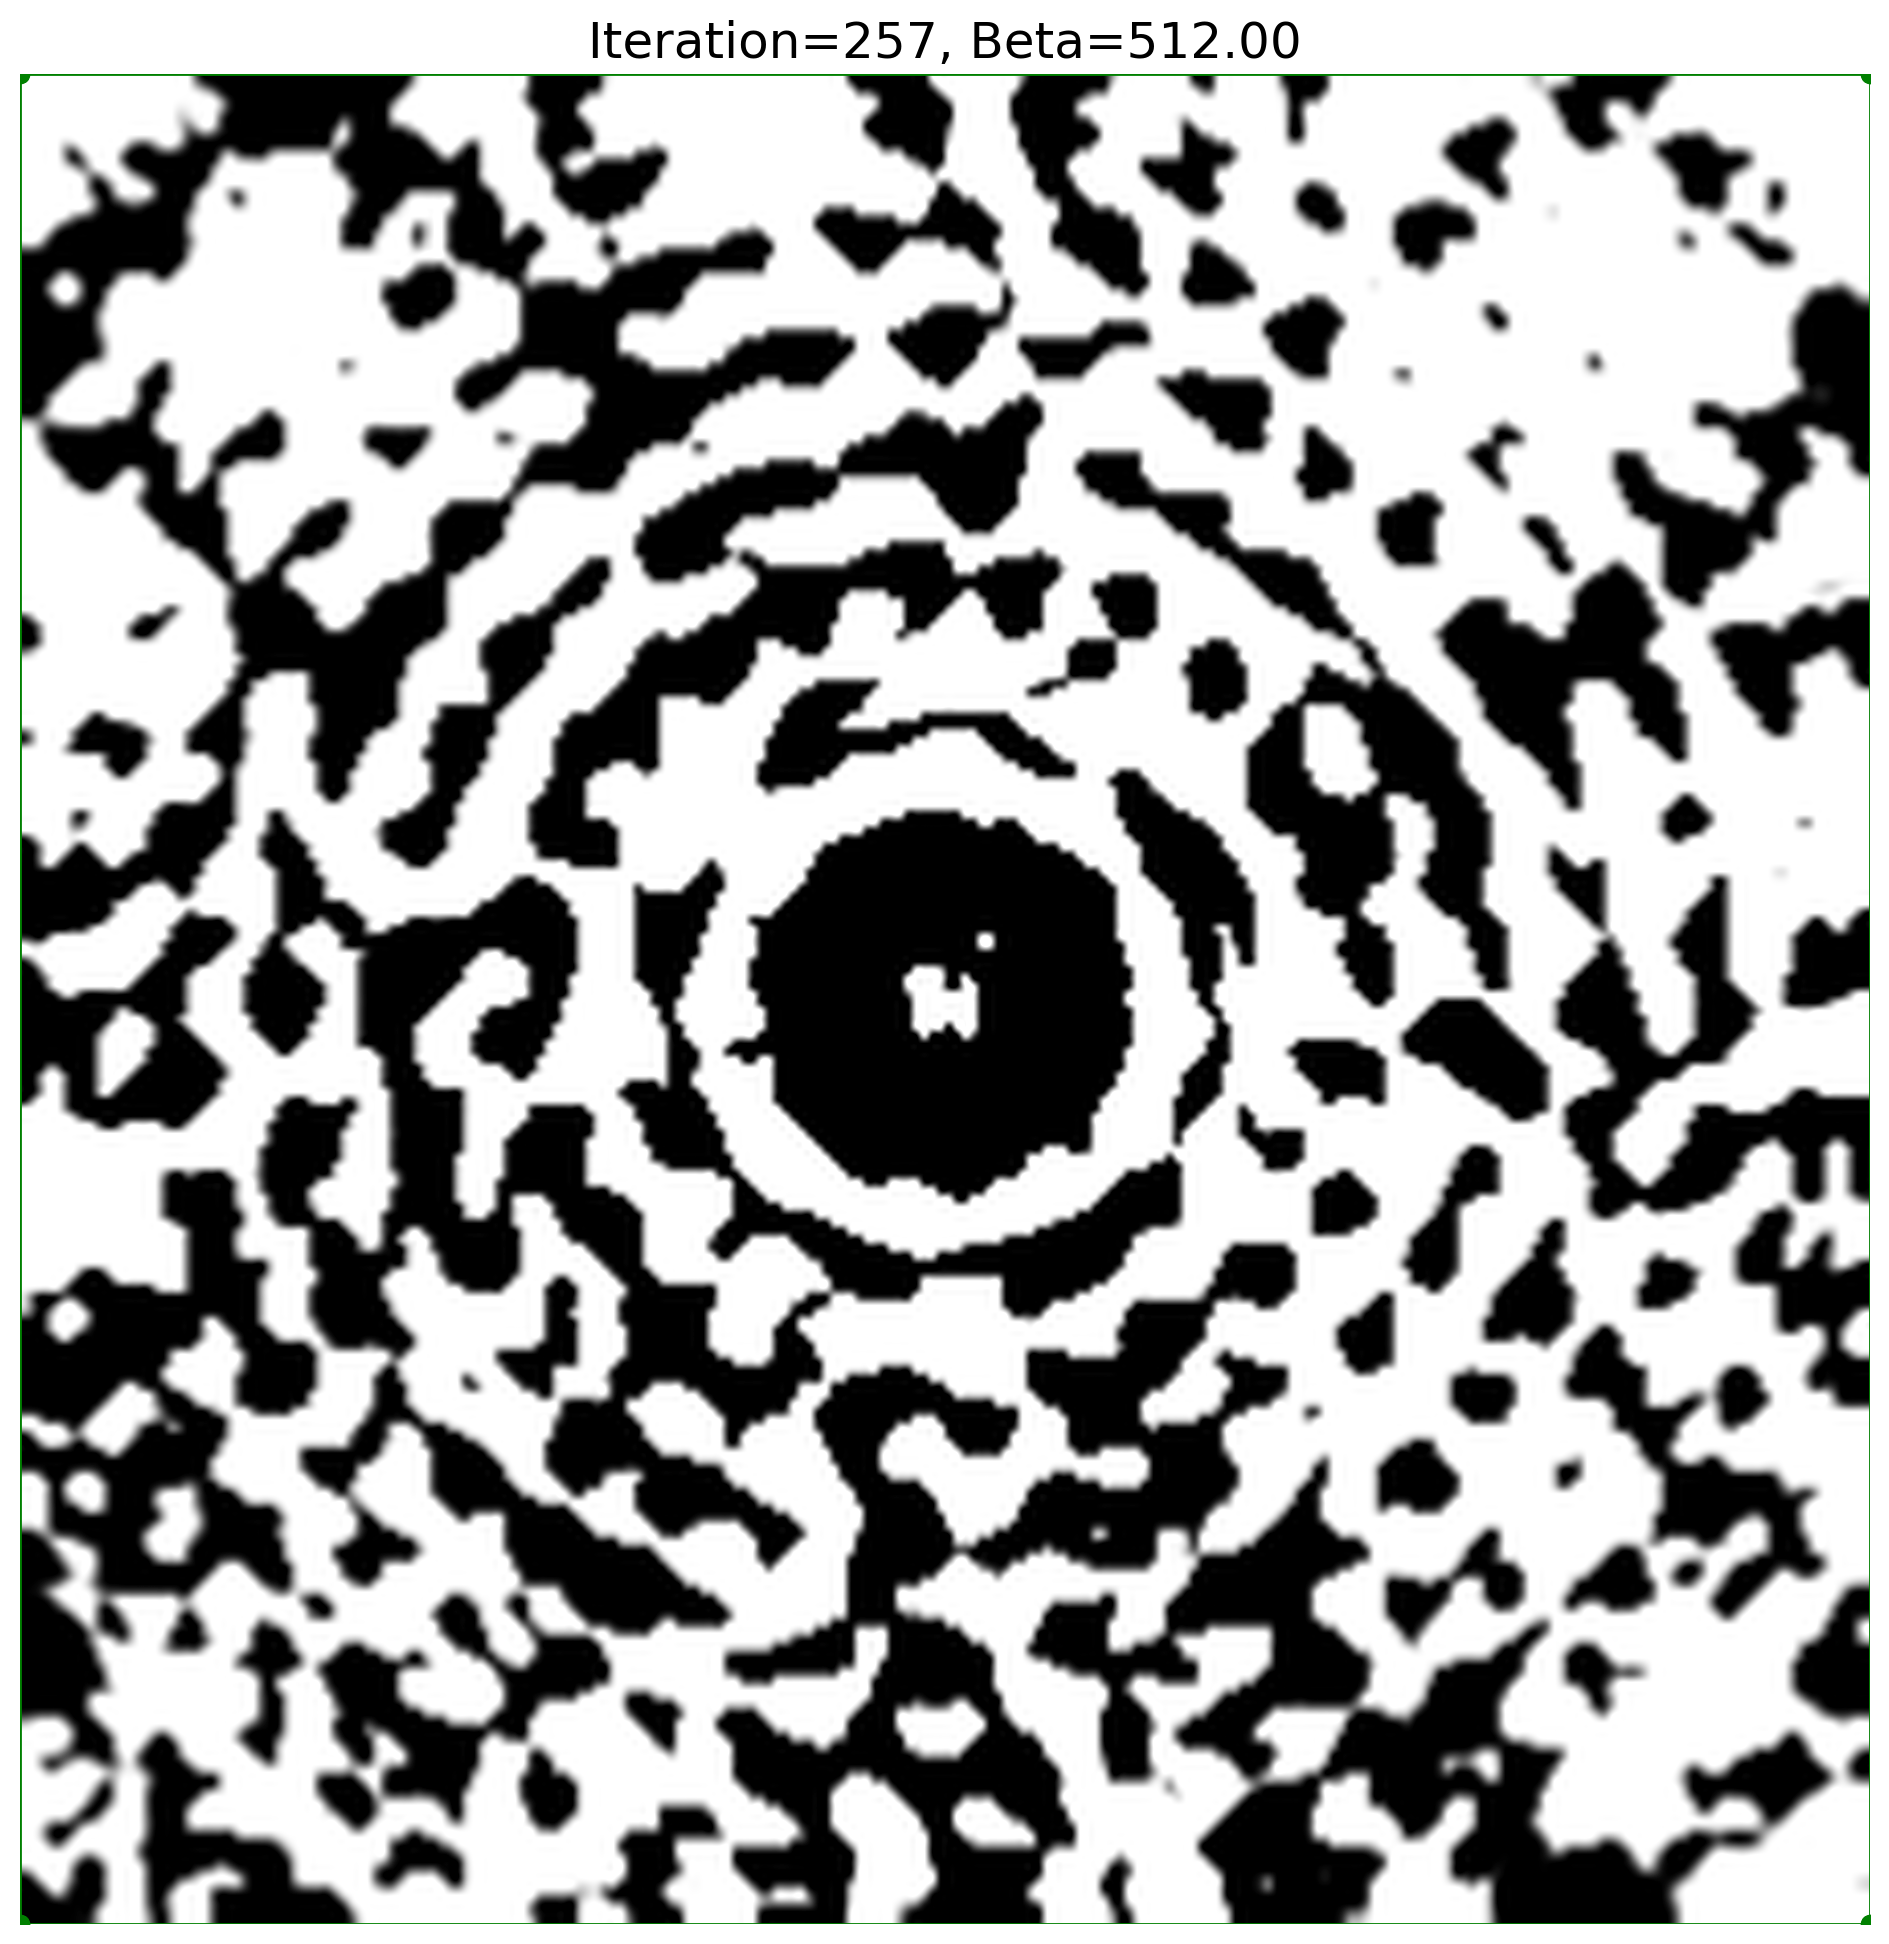
\includegraphics[width=0.3\textwidth]{img/017_structure_iter_257_beta_512.00.png} &
        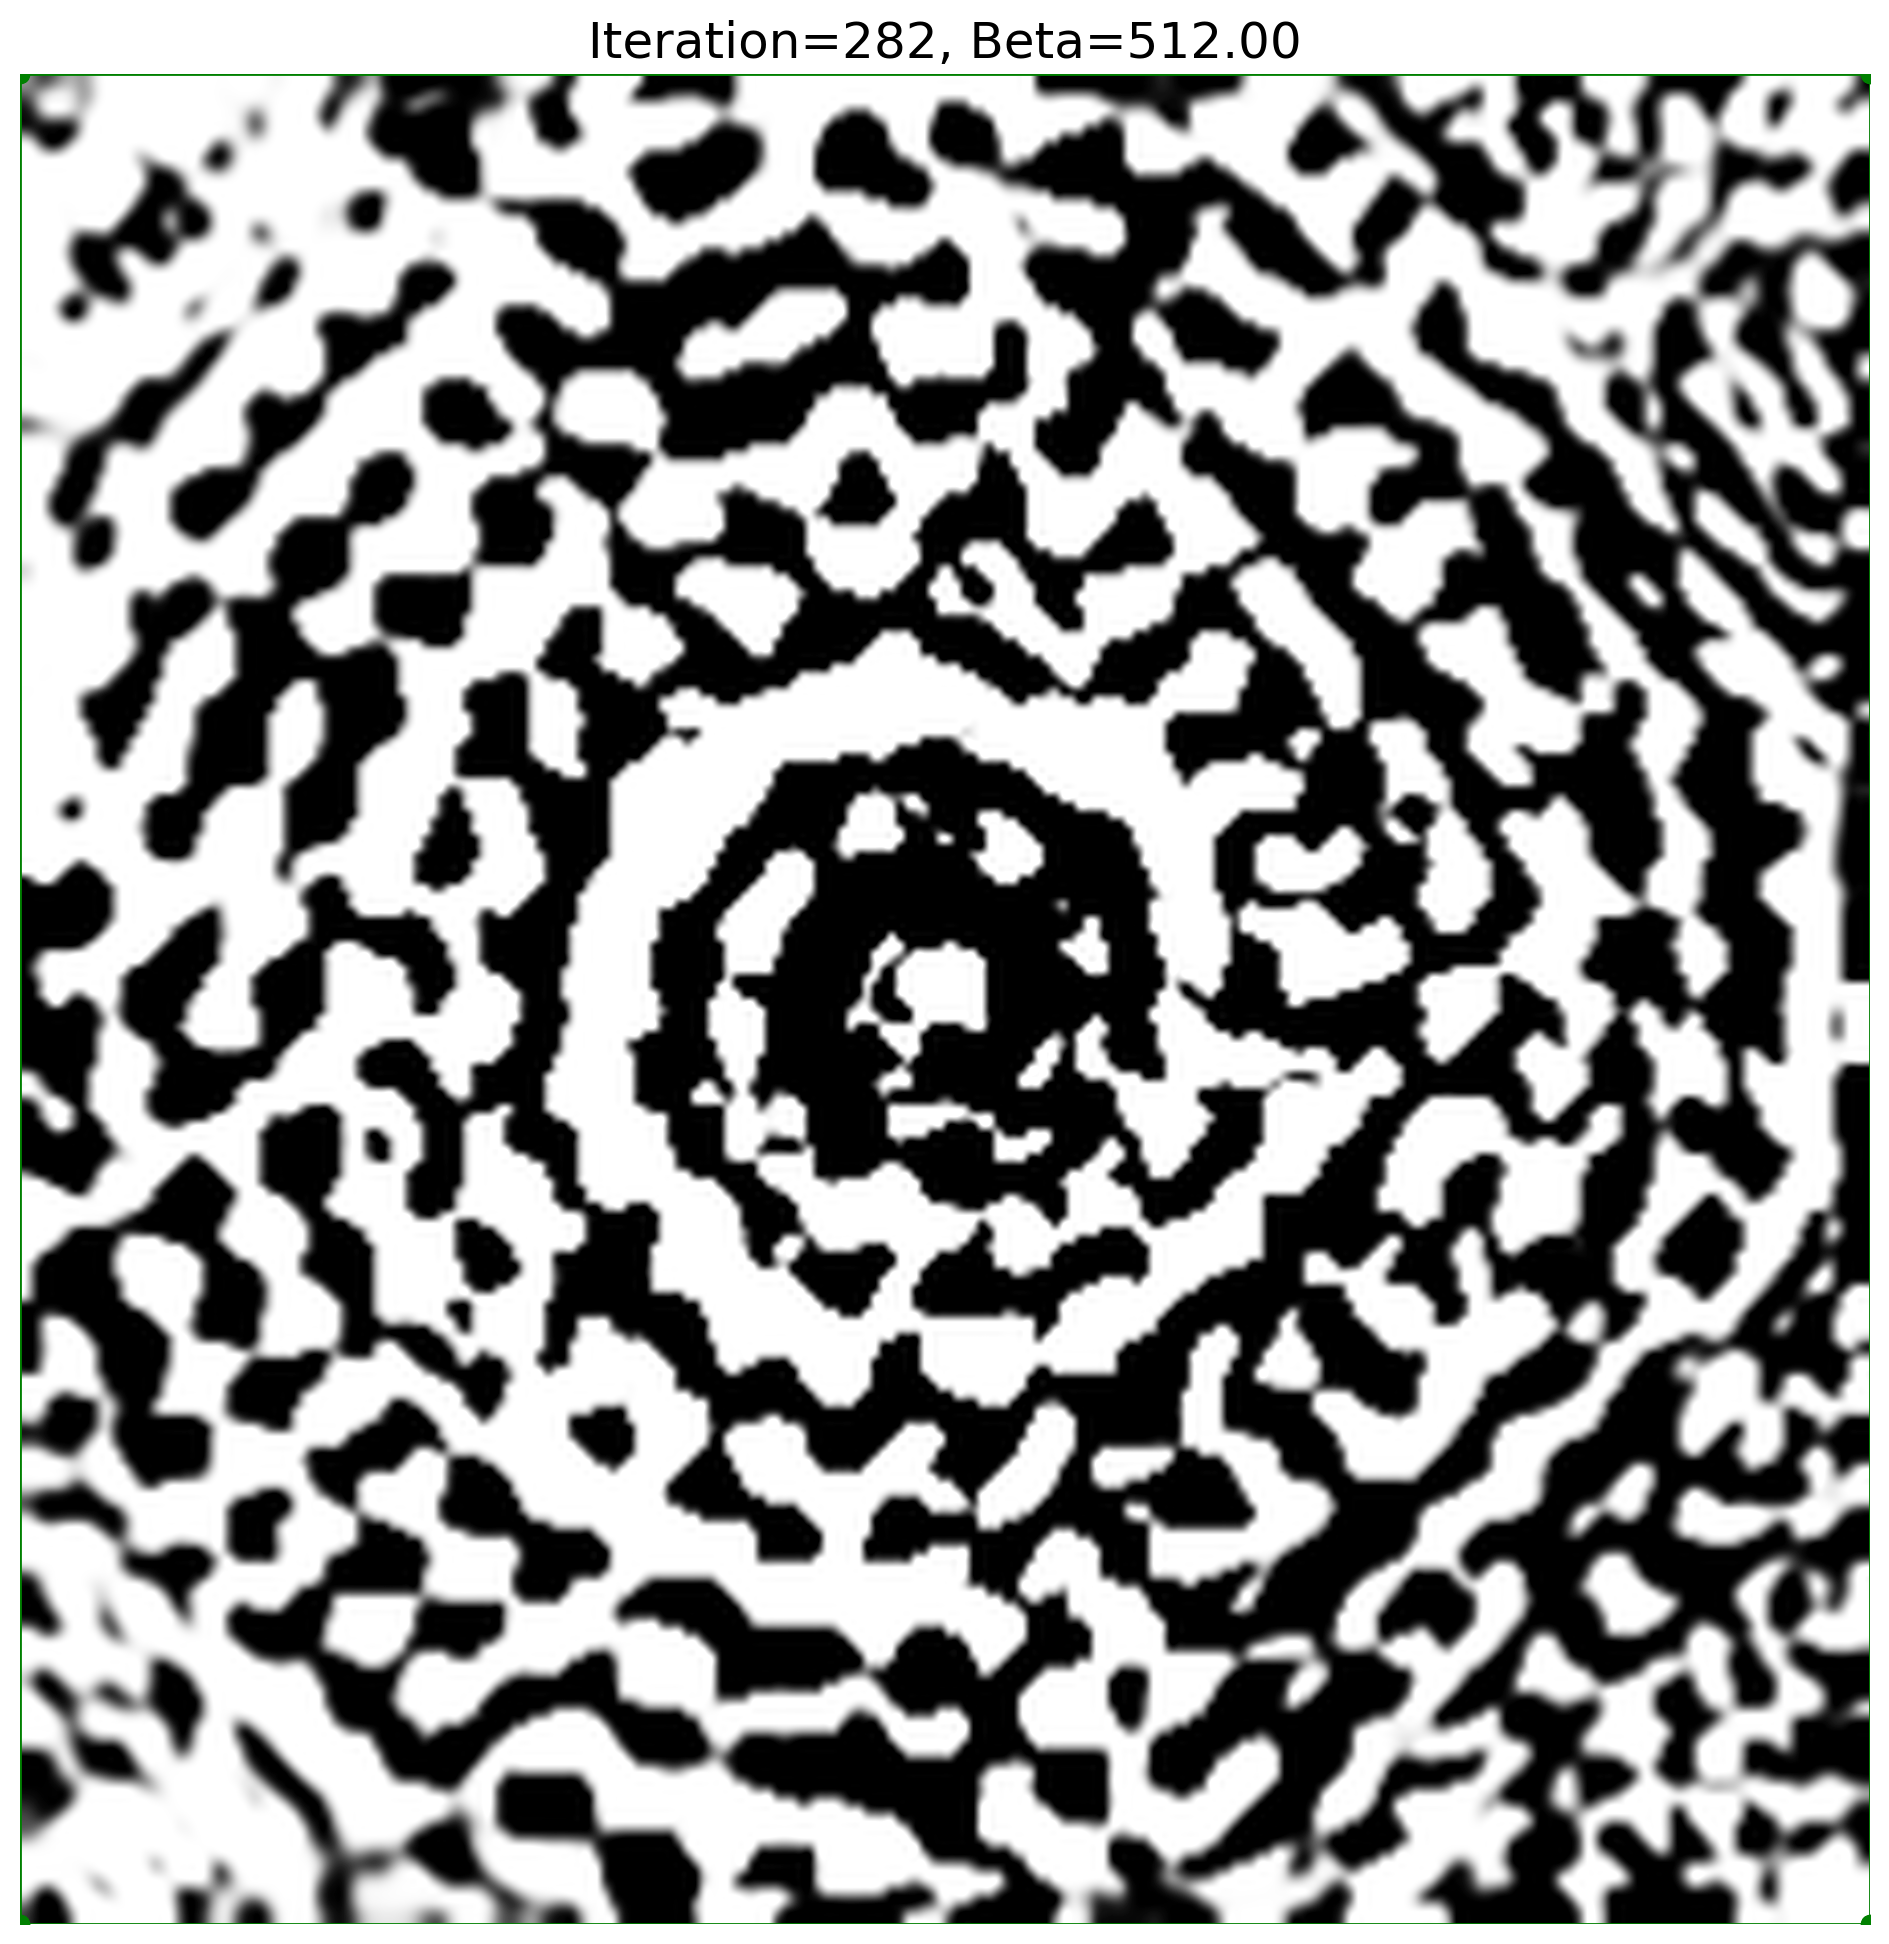
\includegraphics[width=0.3\textwidth]{img/018_structure_iter_282_beta_512.00.png} &
        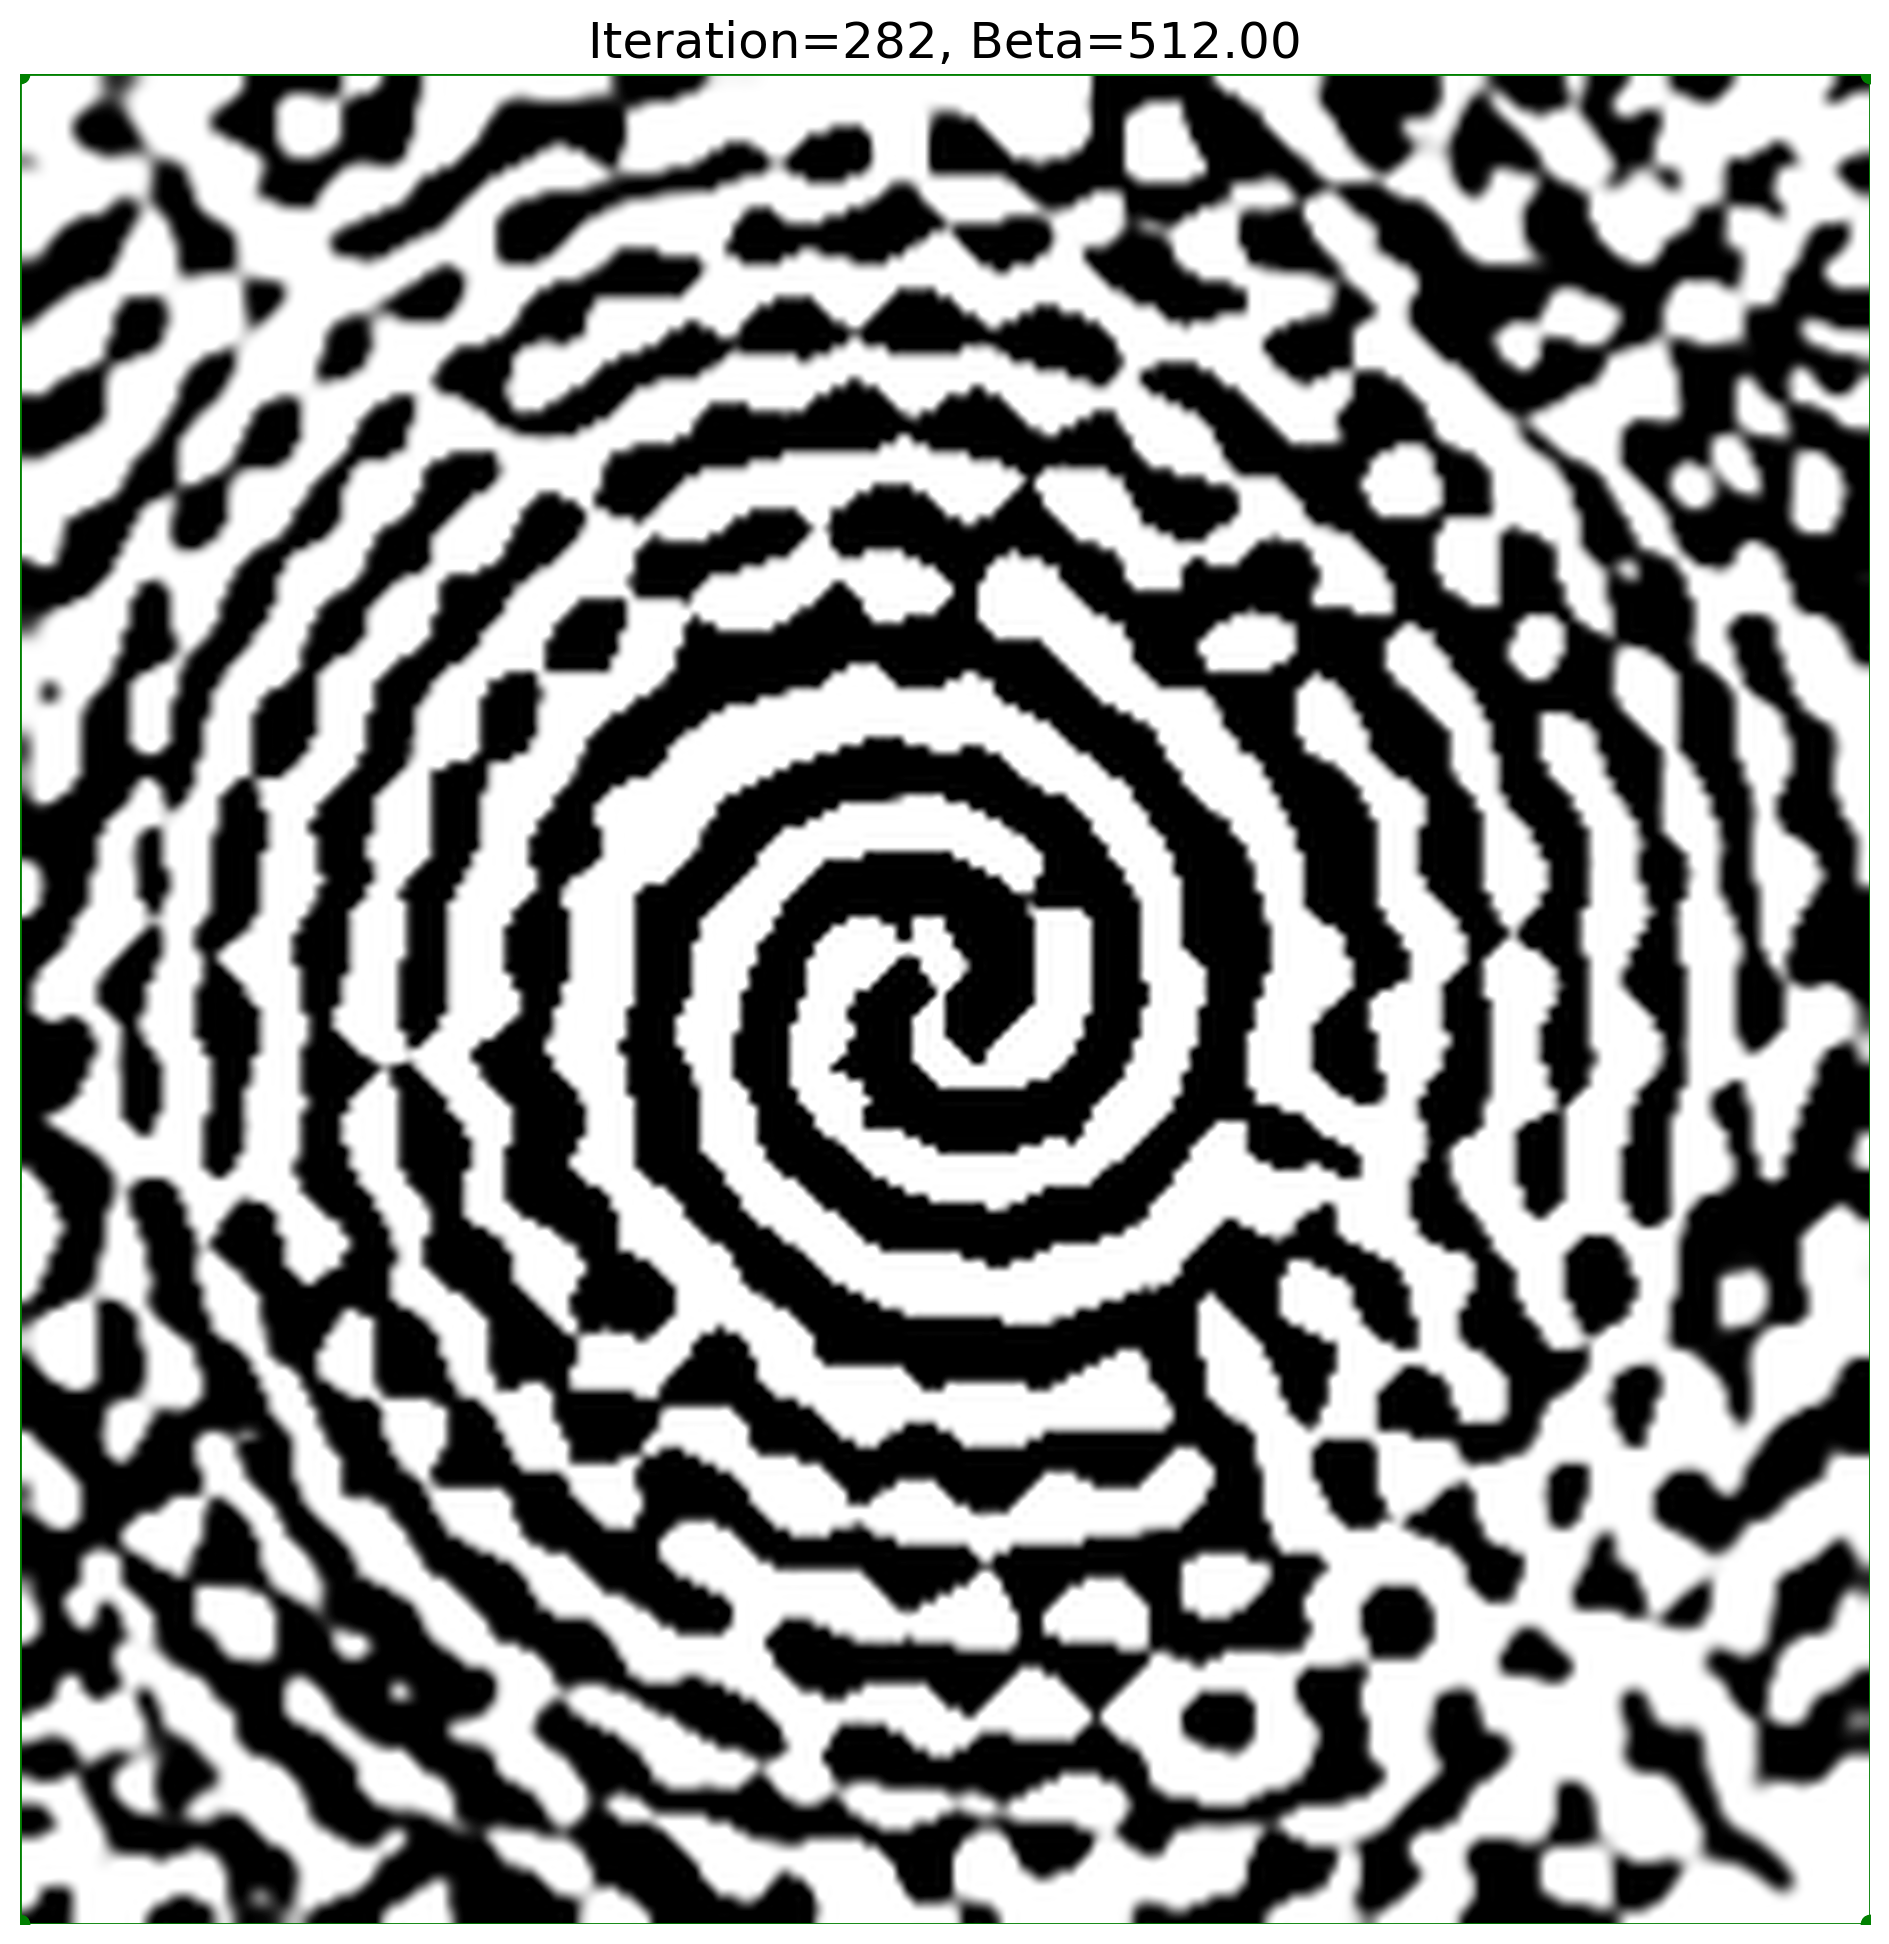
\includegraphics[width=0.3\textwidth]{img/013_structure_iter_282_beta_512.00.png} 
        \\ (a)  &  (b)  &  (c) \\[8pt]
        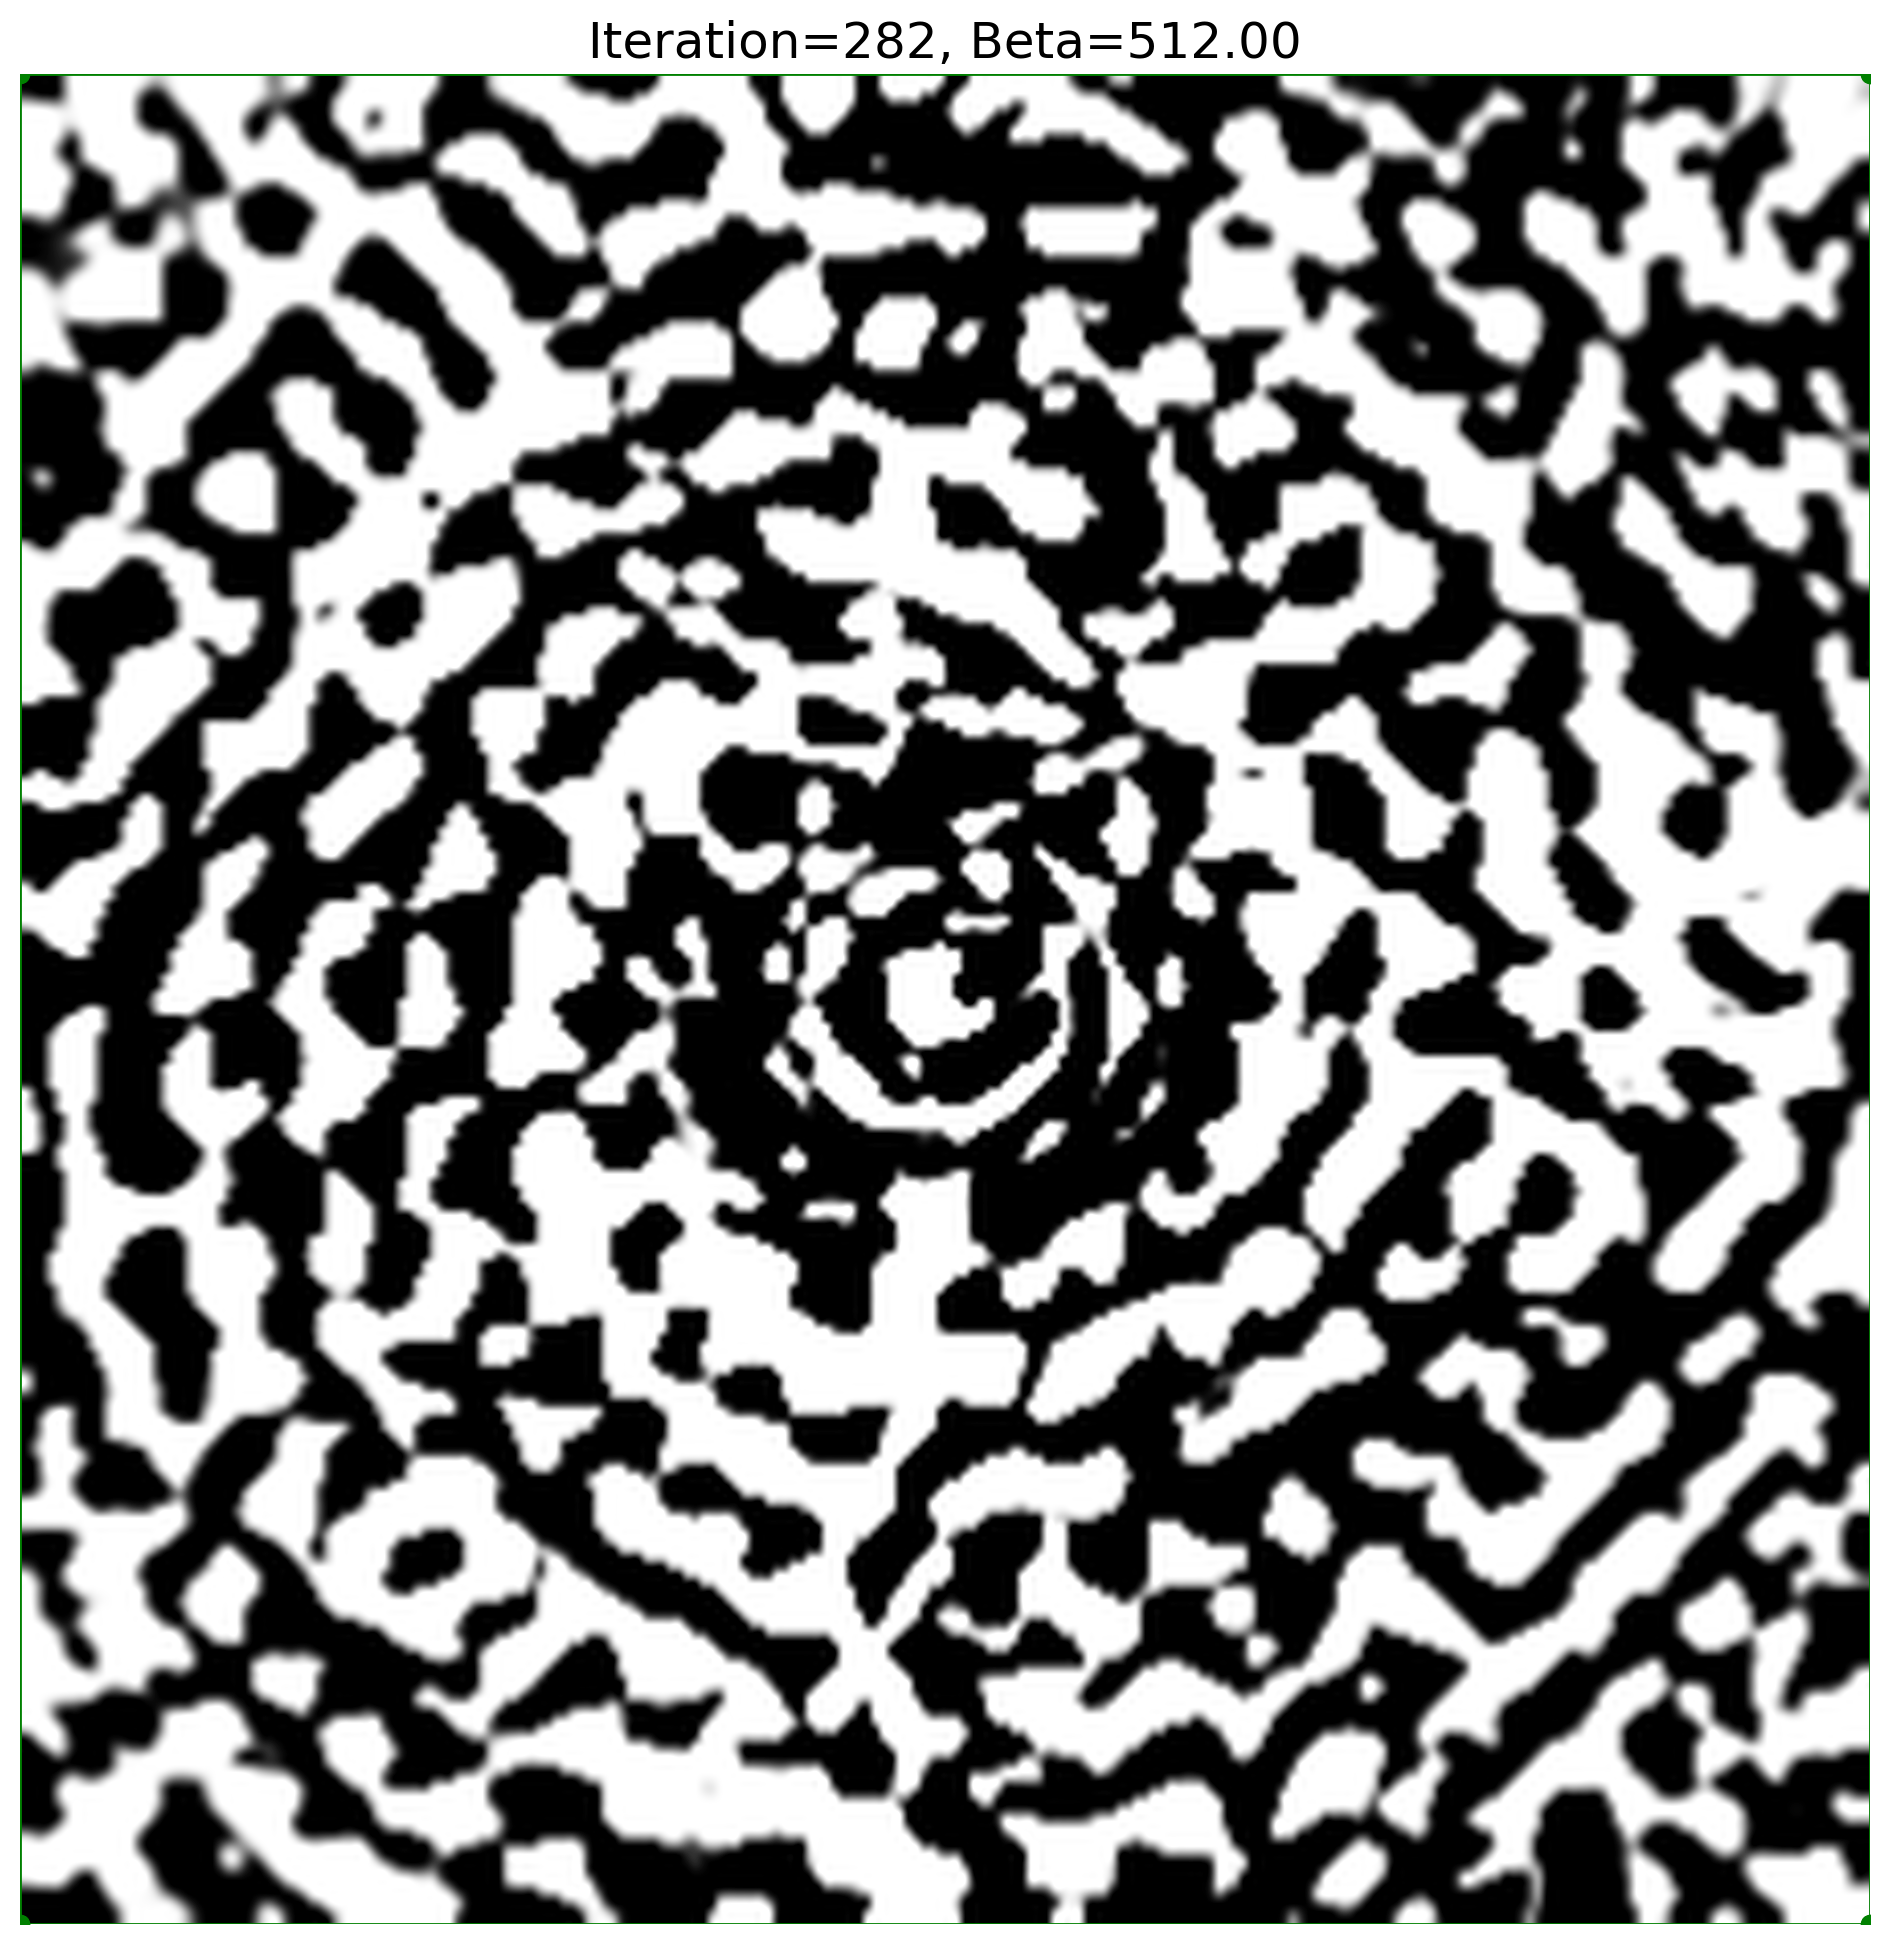
\includegraphics[width=0.3\textwidth]{img/020_structure_iter_282_beta_512.00.png} &
        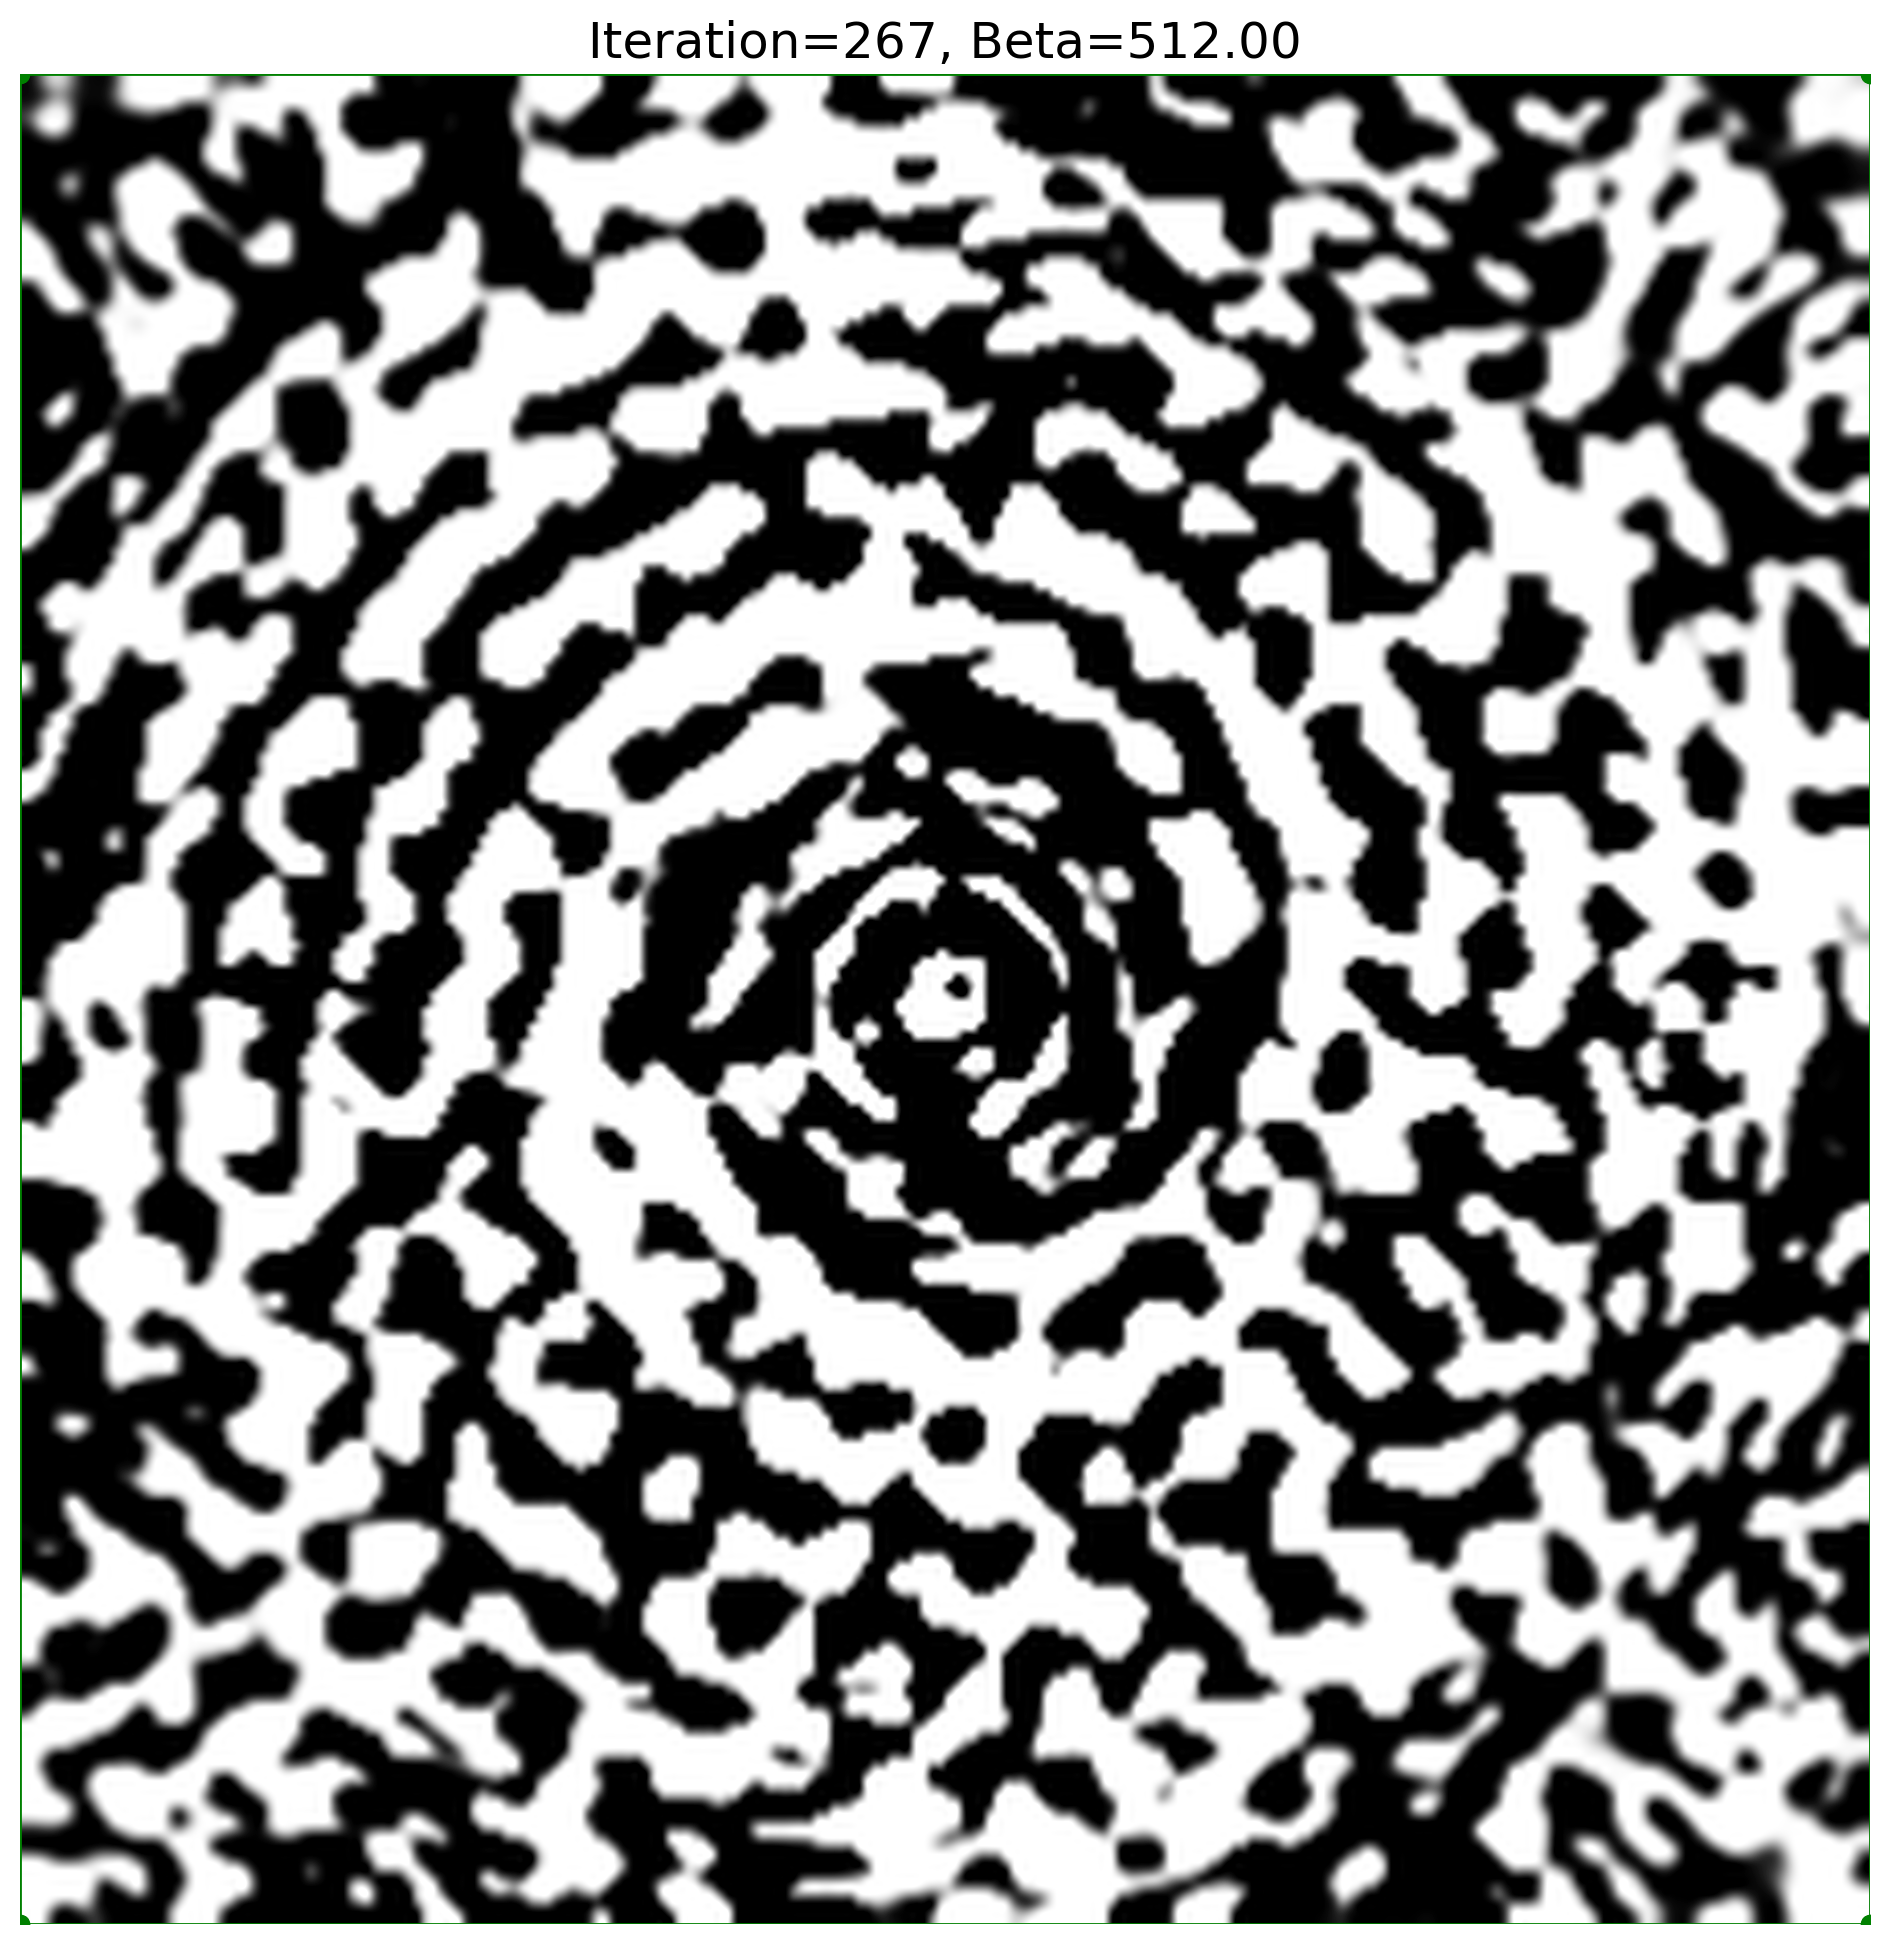
\includegraphics[width=0.3\textwidth]{img/021_structure_iter_267_beta_512.00.png} &
        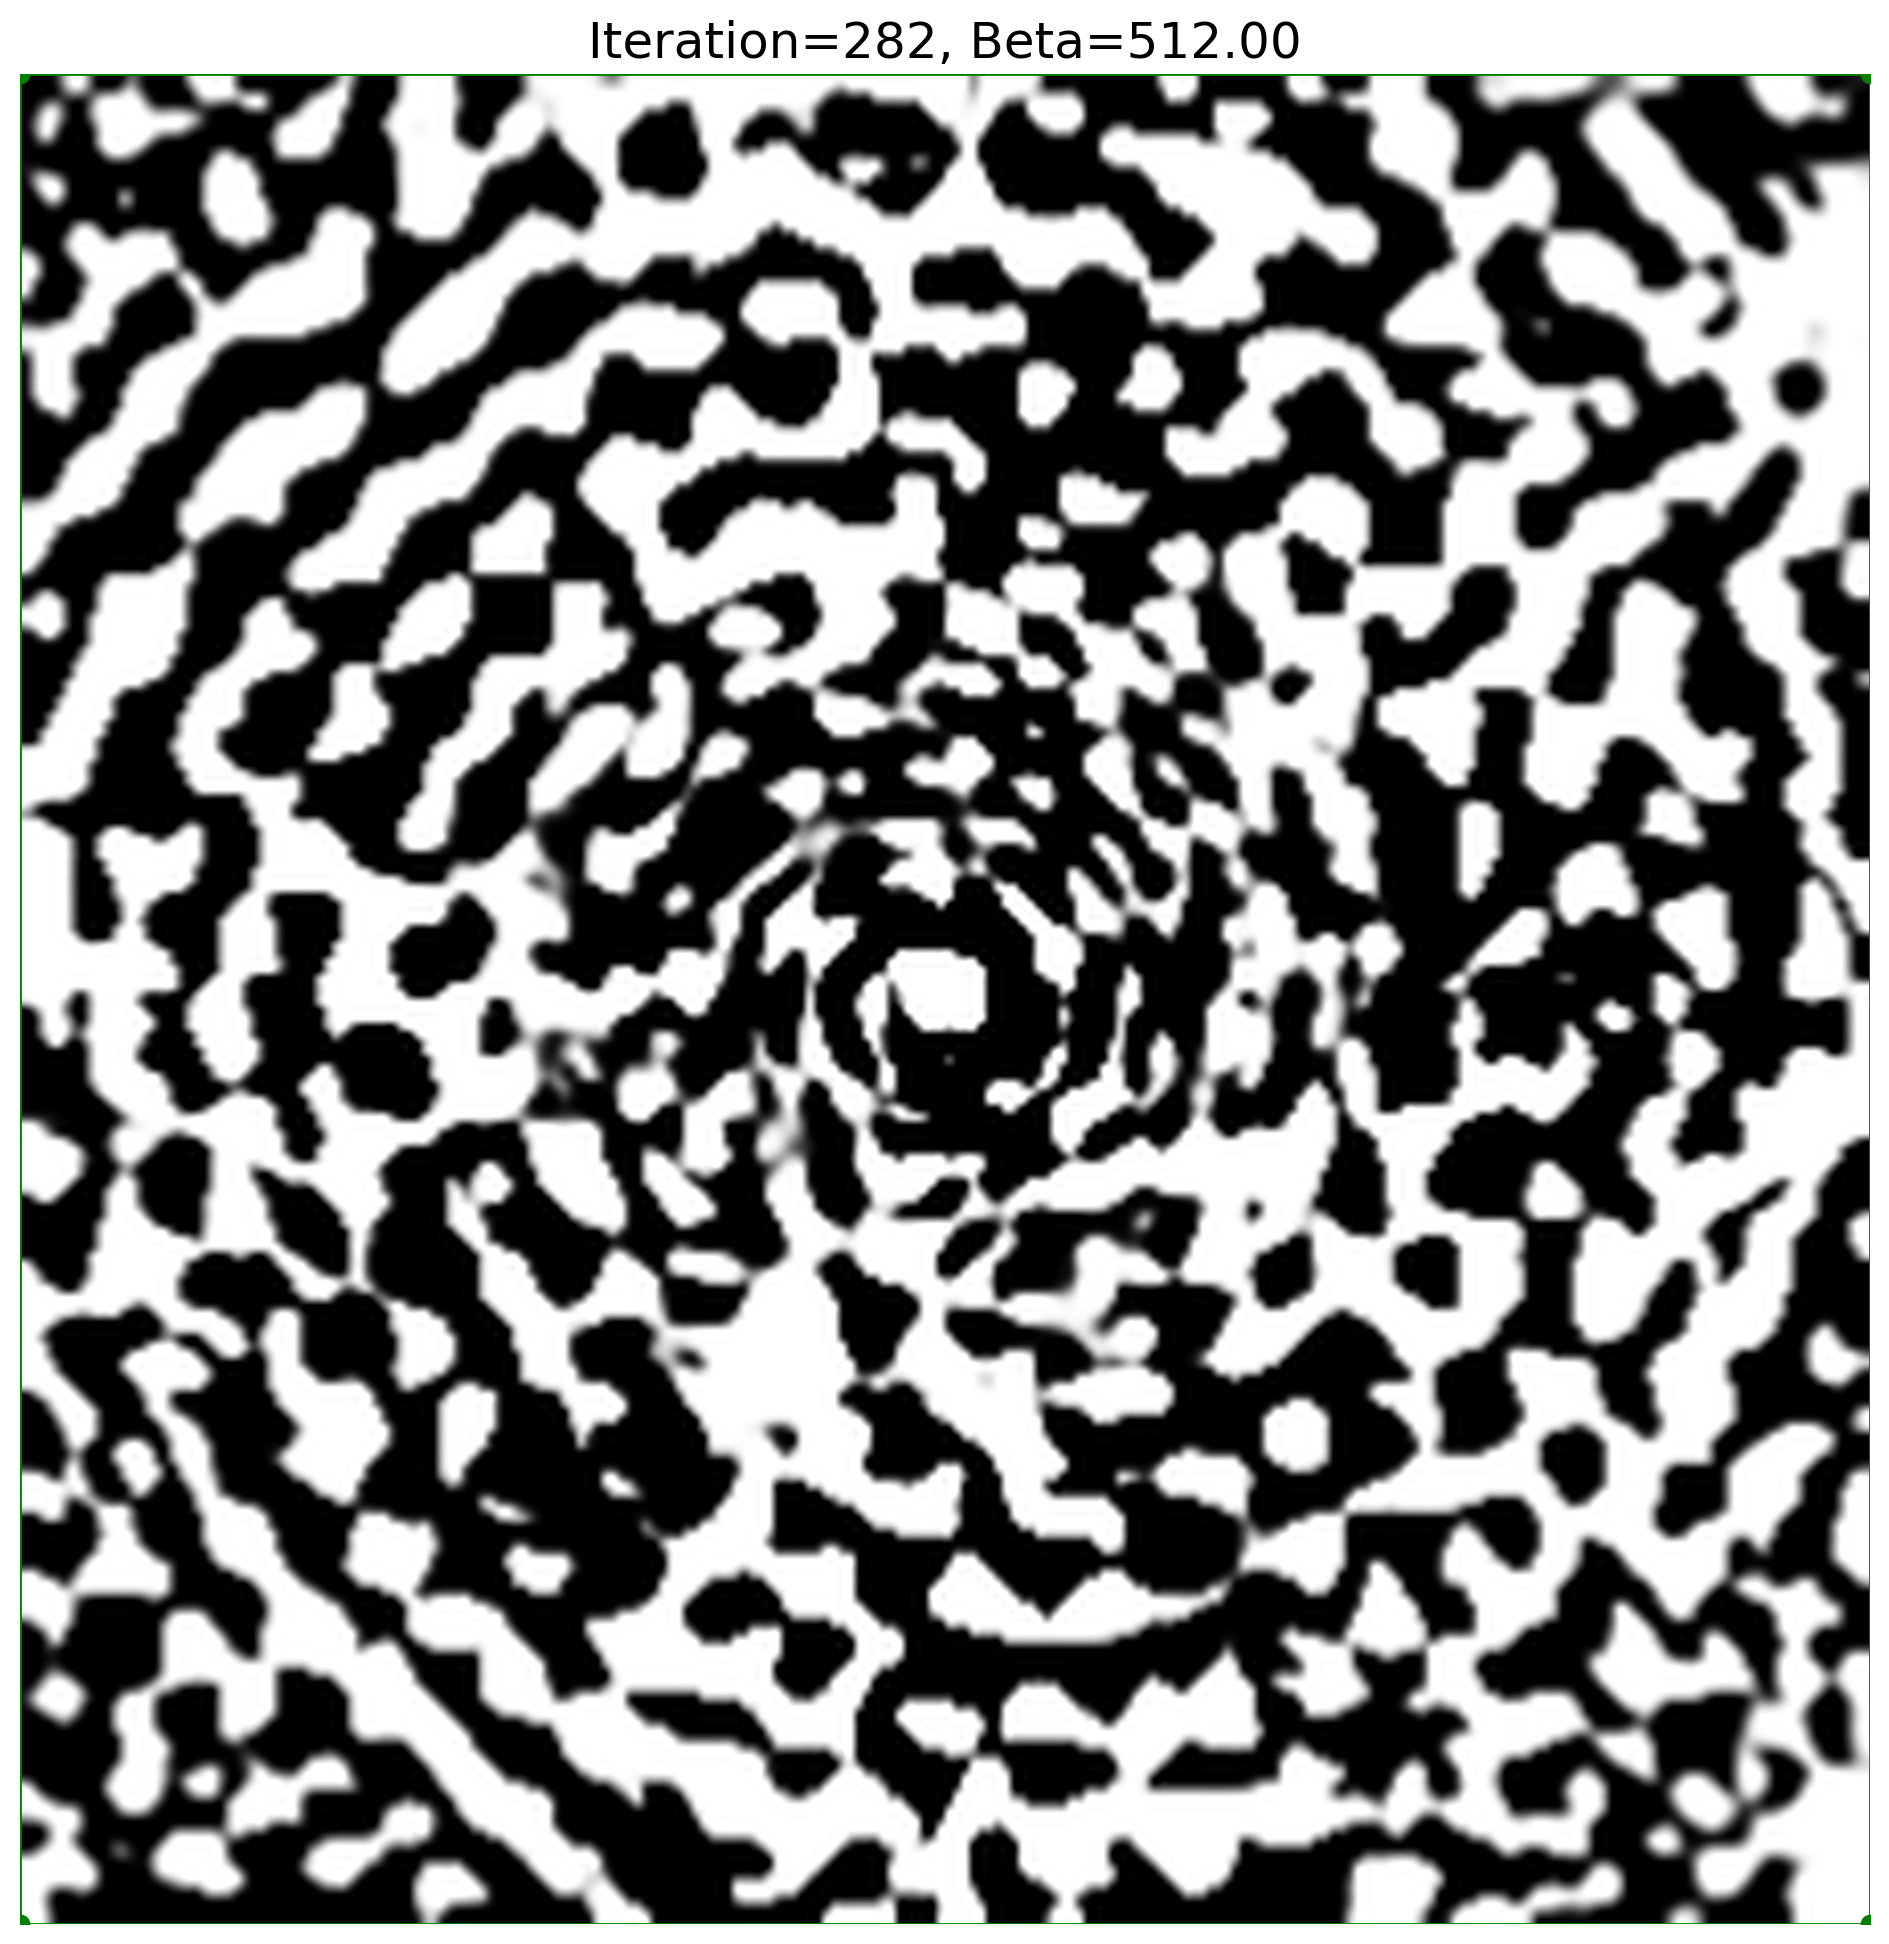
\includegraphics[width=0.3\textwidth]{img/022_structure_iter_282_beta_512.00.png}
        \\(d)  &  (e)  &  (f) 
    \end{tabular}
\caption{Final converged GaP/air binary material density distributions ($\beta = 512$, binarized structures): (a)$\sim$(f) $\ell \in \{0, 1, 2, 3, 4, 5\}$, respectively . Black represents GaP ($n = 3.31$); white represents air ($n = 1$). The $\ell = 2$ design shows a clear two-arm spiral pattern at the center, similar to a spiral phase plate (SPP). The other designs show free-form non-intuitive material distributions that do not follow simple $\ell$-fold rotational symmetry.}
\label{fig:structures_all}

\end{figure}


%===================================================================

\section{Near-Field Characteristics}

\label{sec:nearfield}

Figure~\ref{fig:nearfield_all} shows the LCP and RCP electric field phase and normalized intensity distributions ($|E_\text{LCP}|^2$ and $|E_\text{RCP}|^2$) at the near-field monitor plane just above the design layer for the six designs.

The LCP intensity distribution (upper right of each group) is concentrated in the central region of the structure ($\sim 1\;\mu\text{m}$ scale) for all designs, showing non-uniform localized enhancement that reflects the near-field collection efficiency of the optimized structure for LCP dipole radiation. The LCP phase distribution (upper left of each group) shows a complex spatial pattern due to structural scattering—a stark contrast to the ordered spiral phase in the far field—indicating that near-field phase modulation arises from the collective action of scattering effects rather than local phase delay.

The RCP component (bottom row of each group) has clearly lower intensity than the LCP component; the normalized intensity ratio between the two directly reflects the structure's circular polarization selectivity (see Section~\ref{sec:pol_selectivity}). The RCP intensity distribution pattern varies across designs but shows no concentrated near-field enhancement like LCP in any case, indicating that the optimized structure indeed exhibits selective near-field coupling to the K-valley LCP radiation.

\begin{figure}[htb]
\centering
	\begin{tabular}{cc} 
	    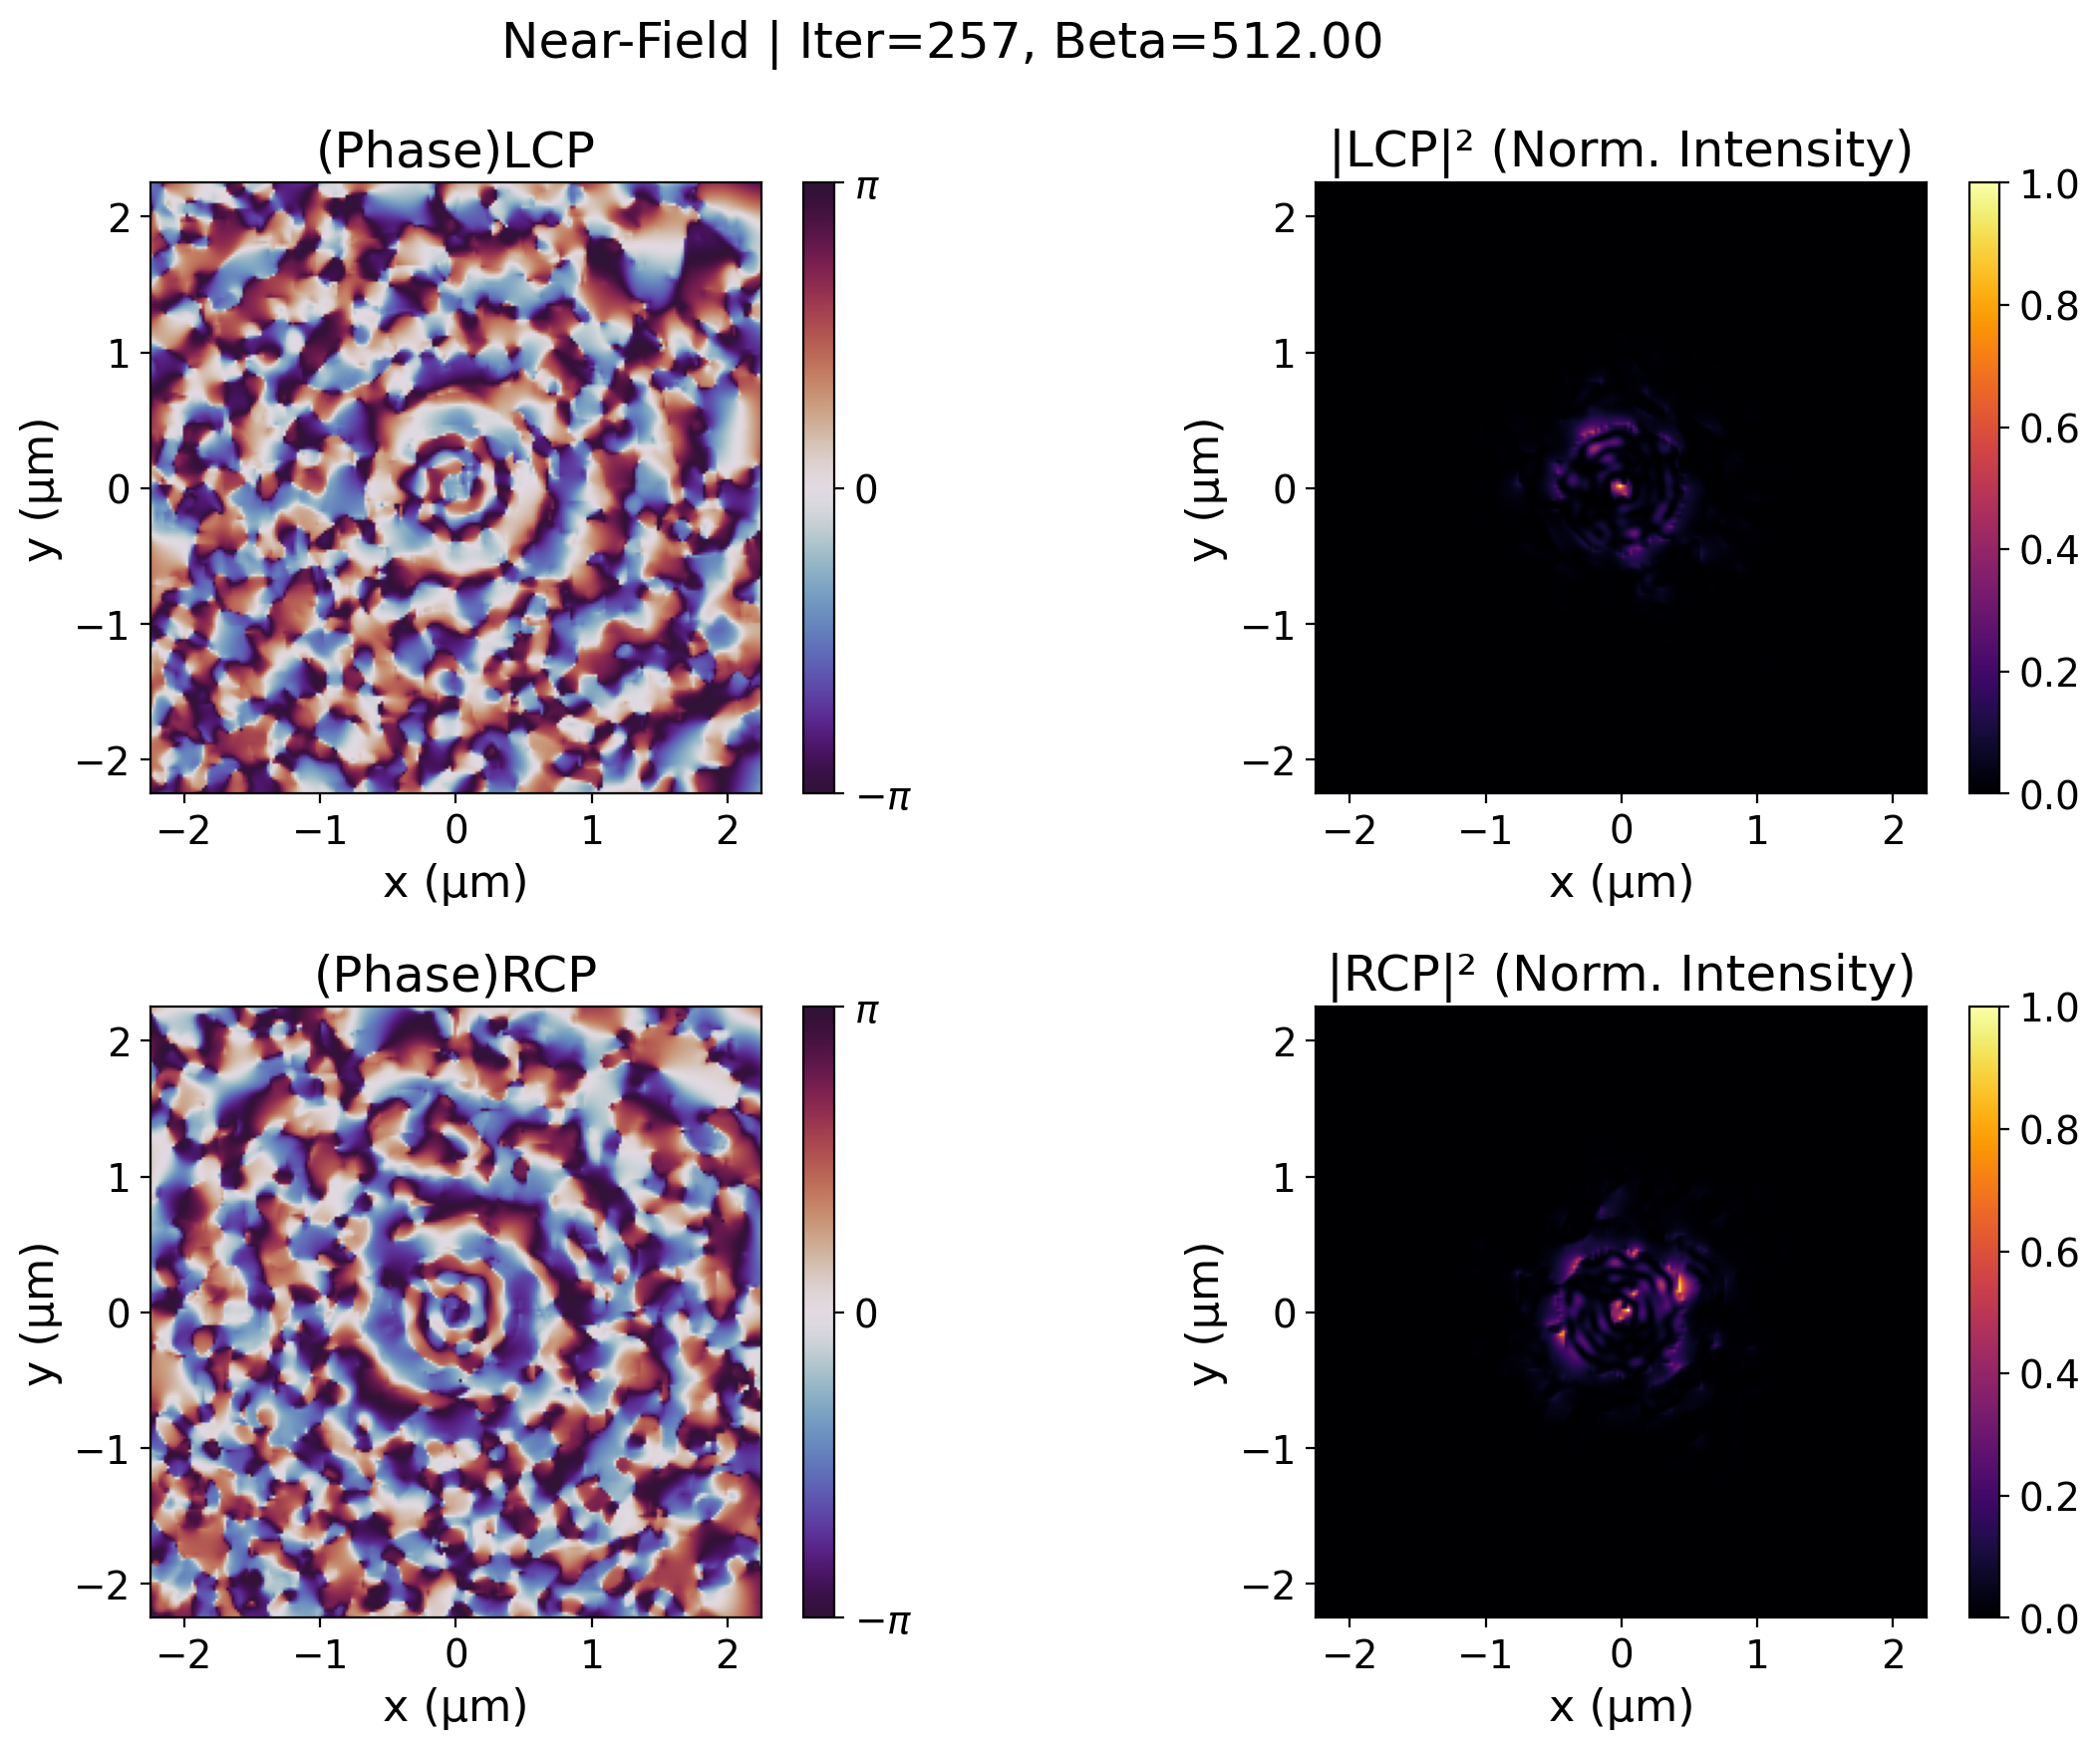
\includegraphics[width=0.47\textwidth]{img/017_phase_iter_257_beta_512.00.png}&
	    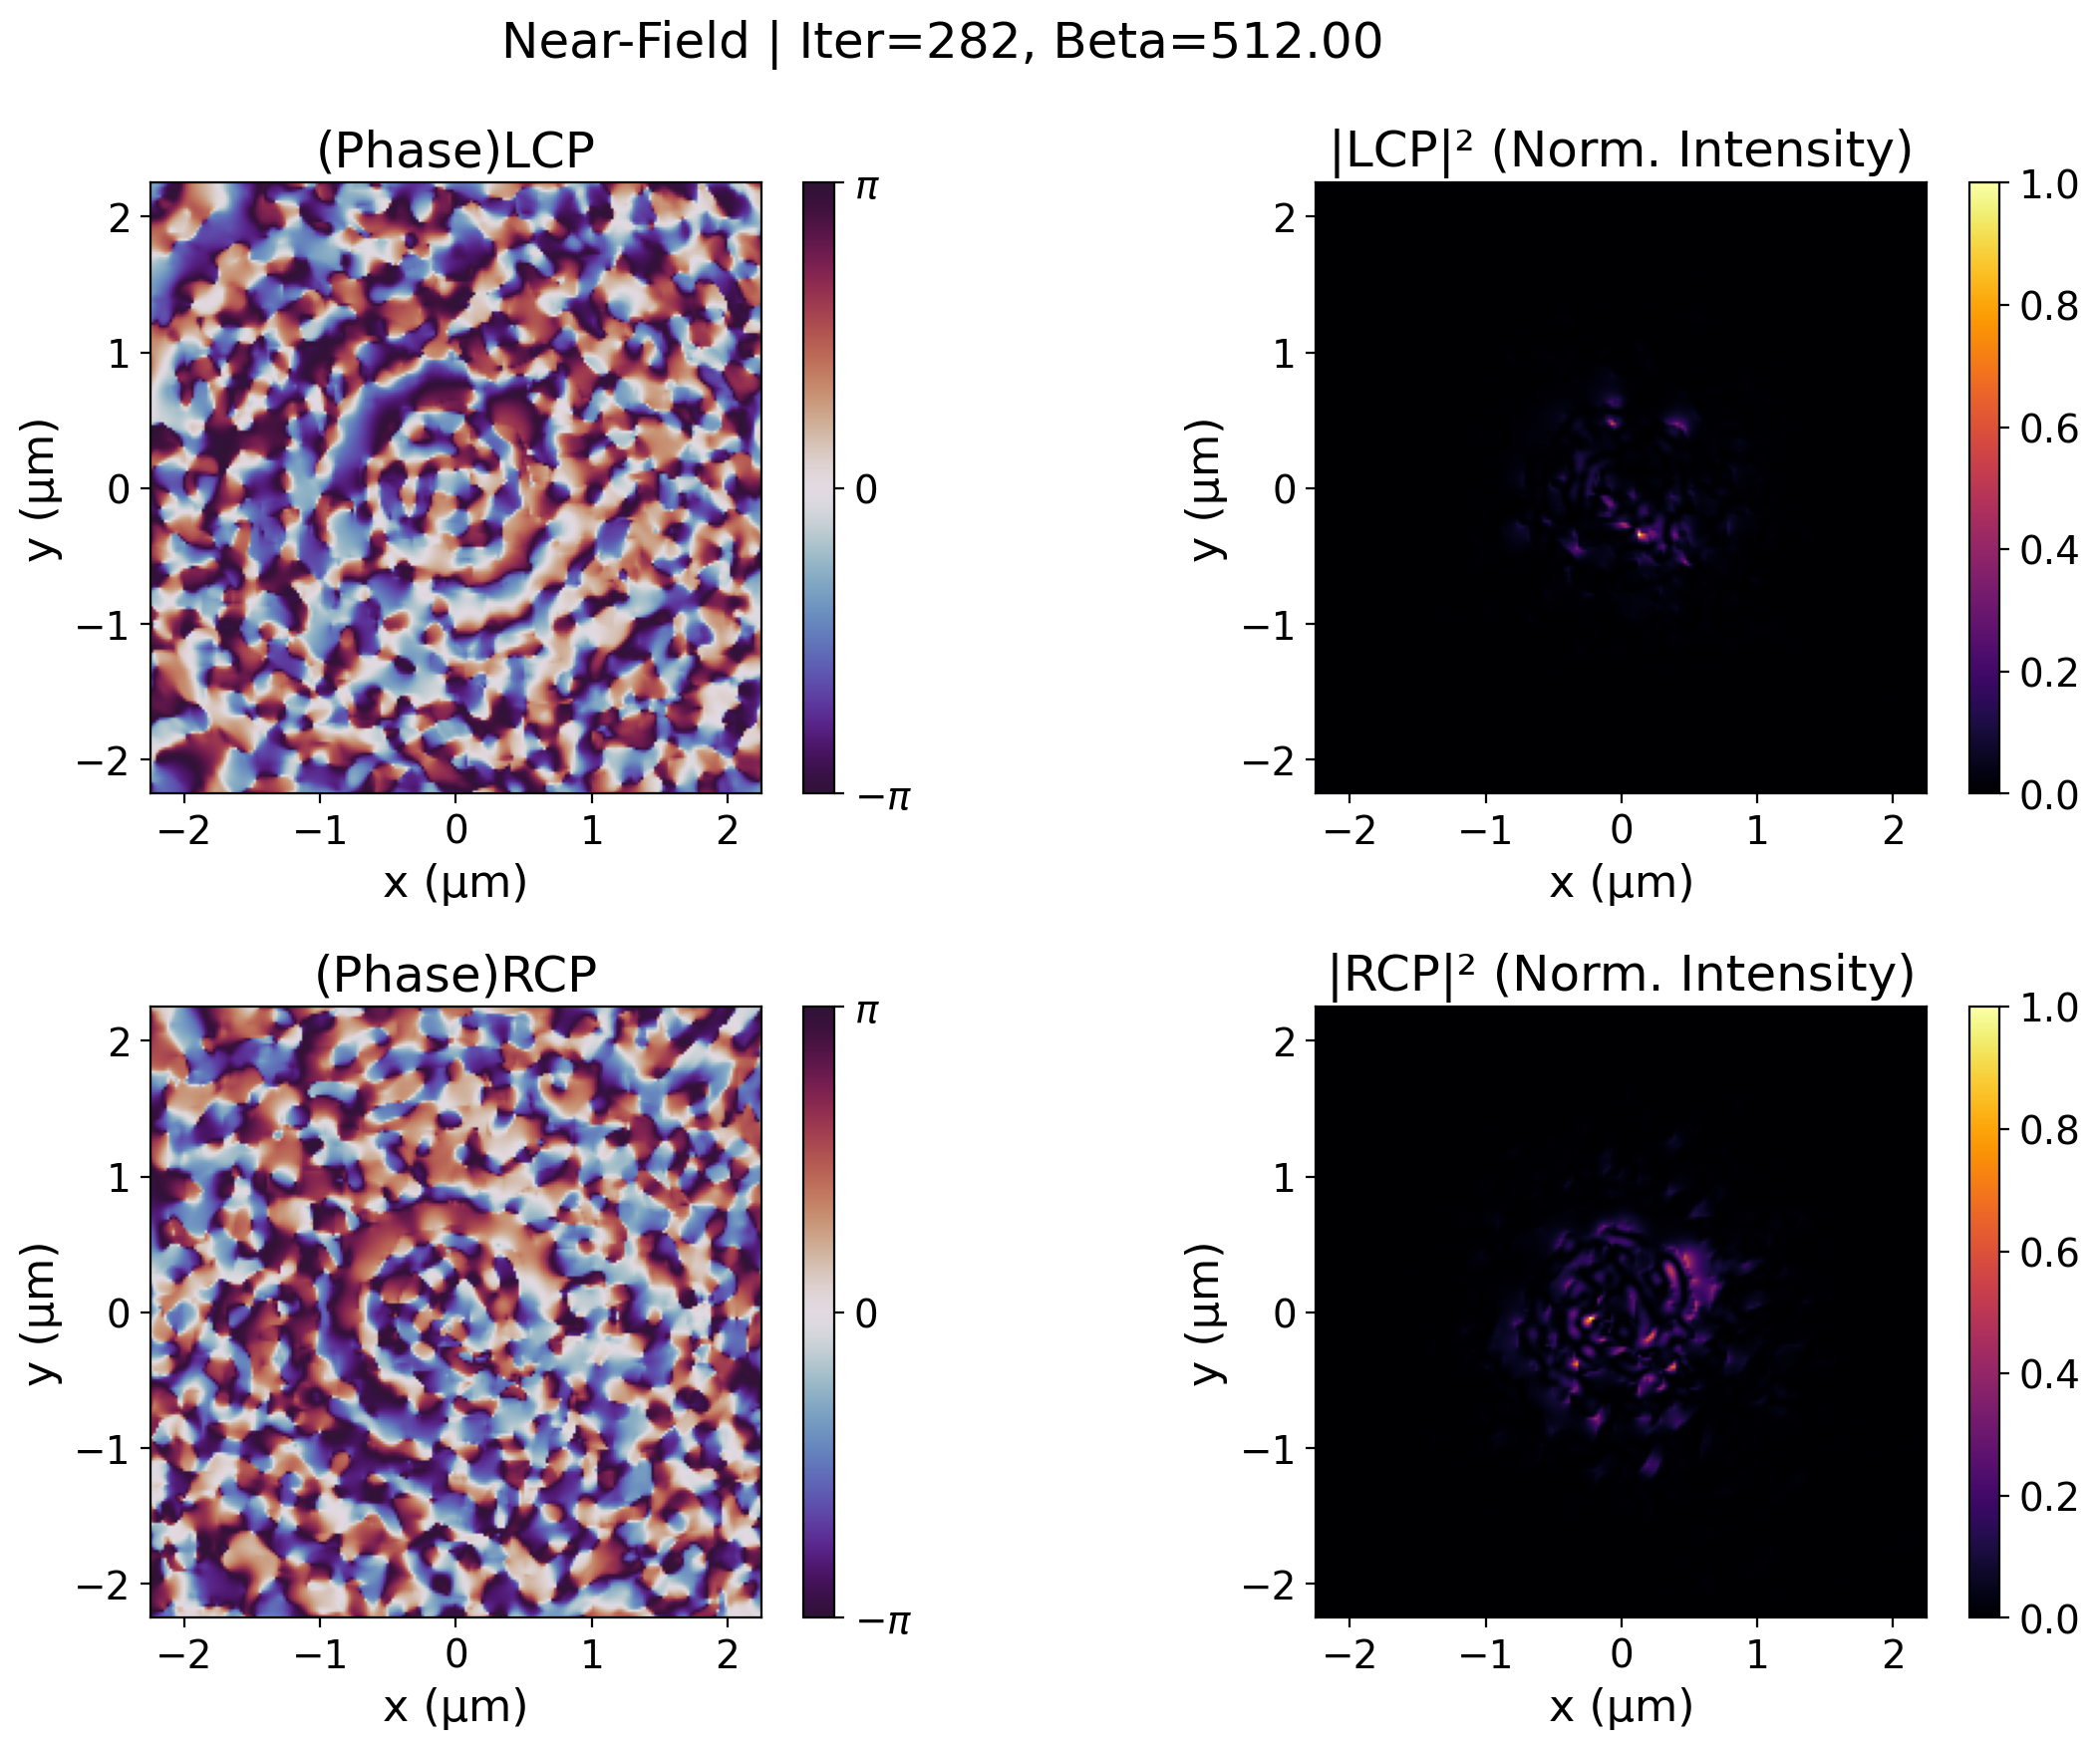
\includegraphics[width=0.47\textwidth]{img/018_phase_iter_282_beta_512.00.png}
		\\ (a)  & (b) \\[6pt]
		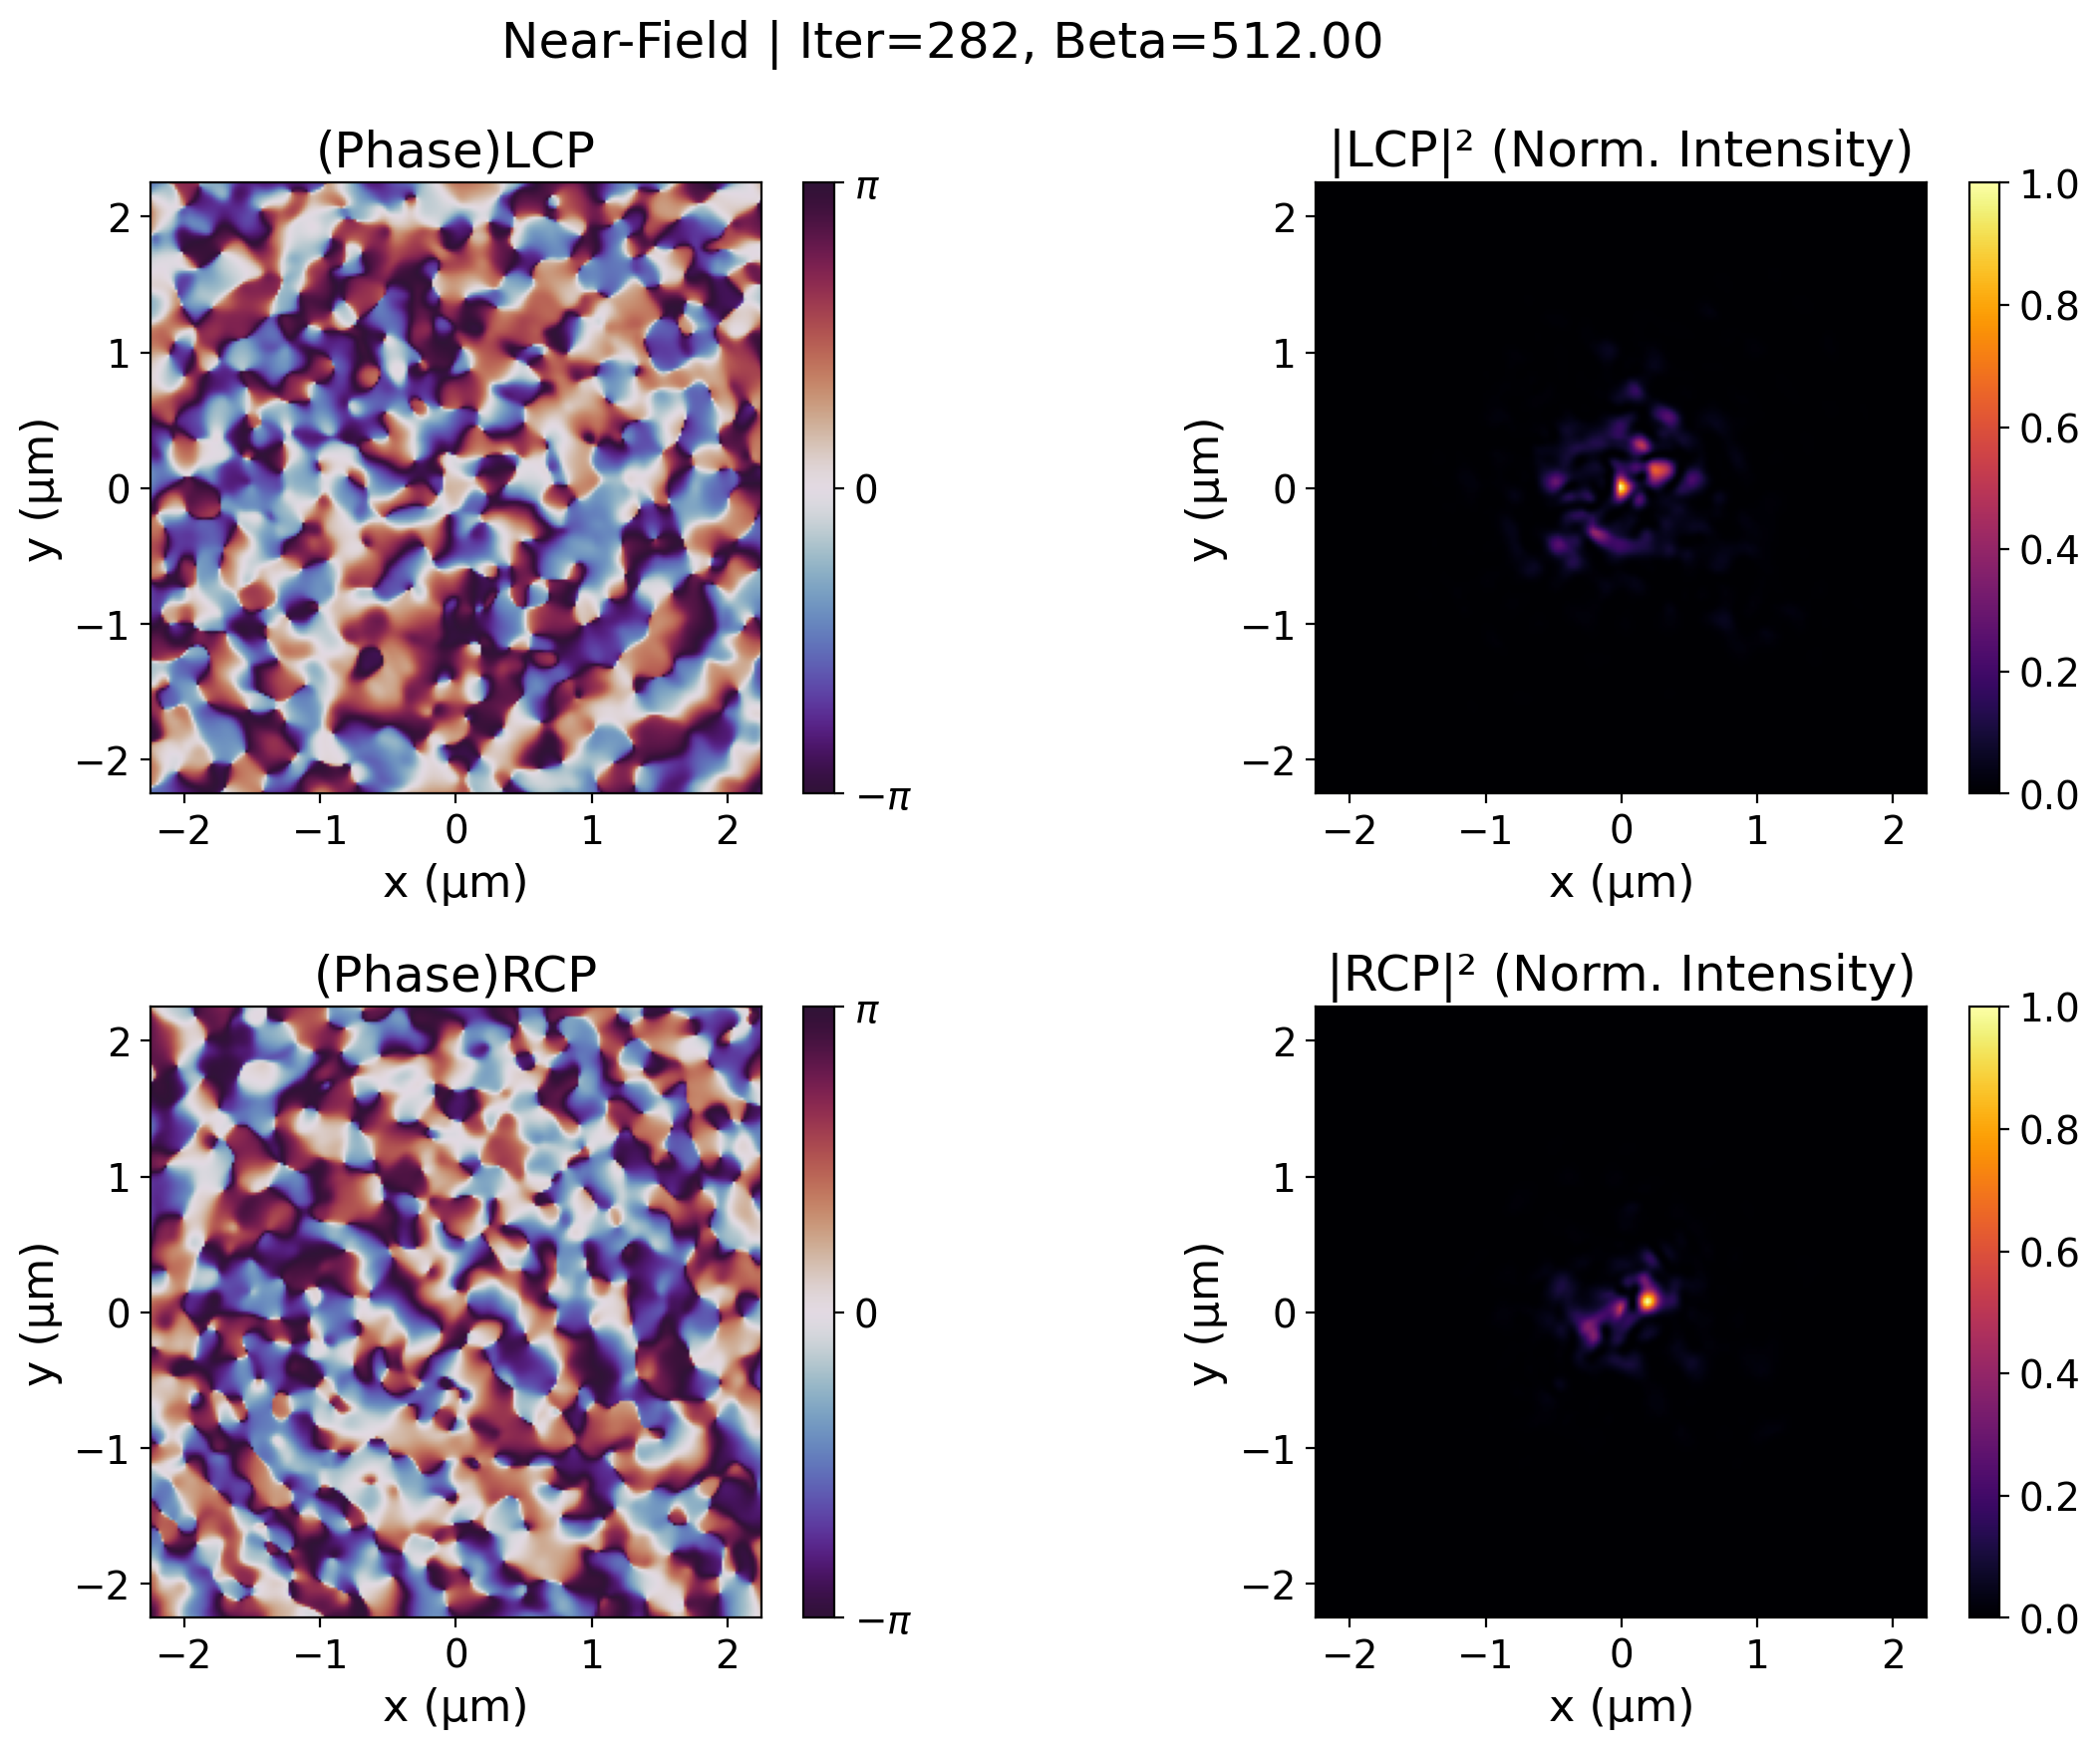
\includegraphics[width=0.47\textwidth]{img/013_phase_iter_282_beta_512.00.png}&
	    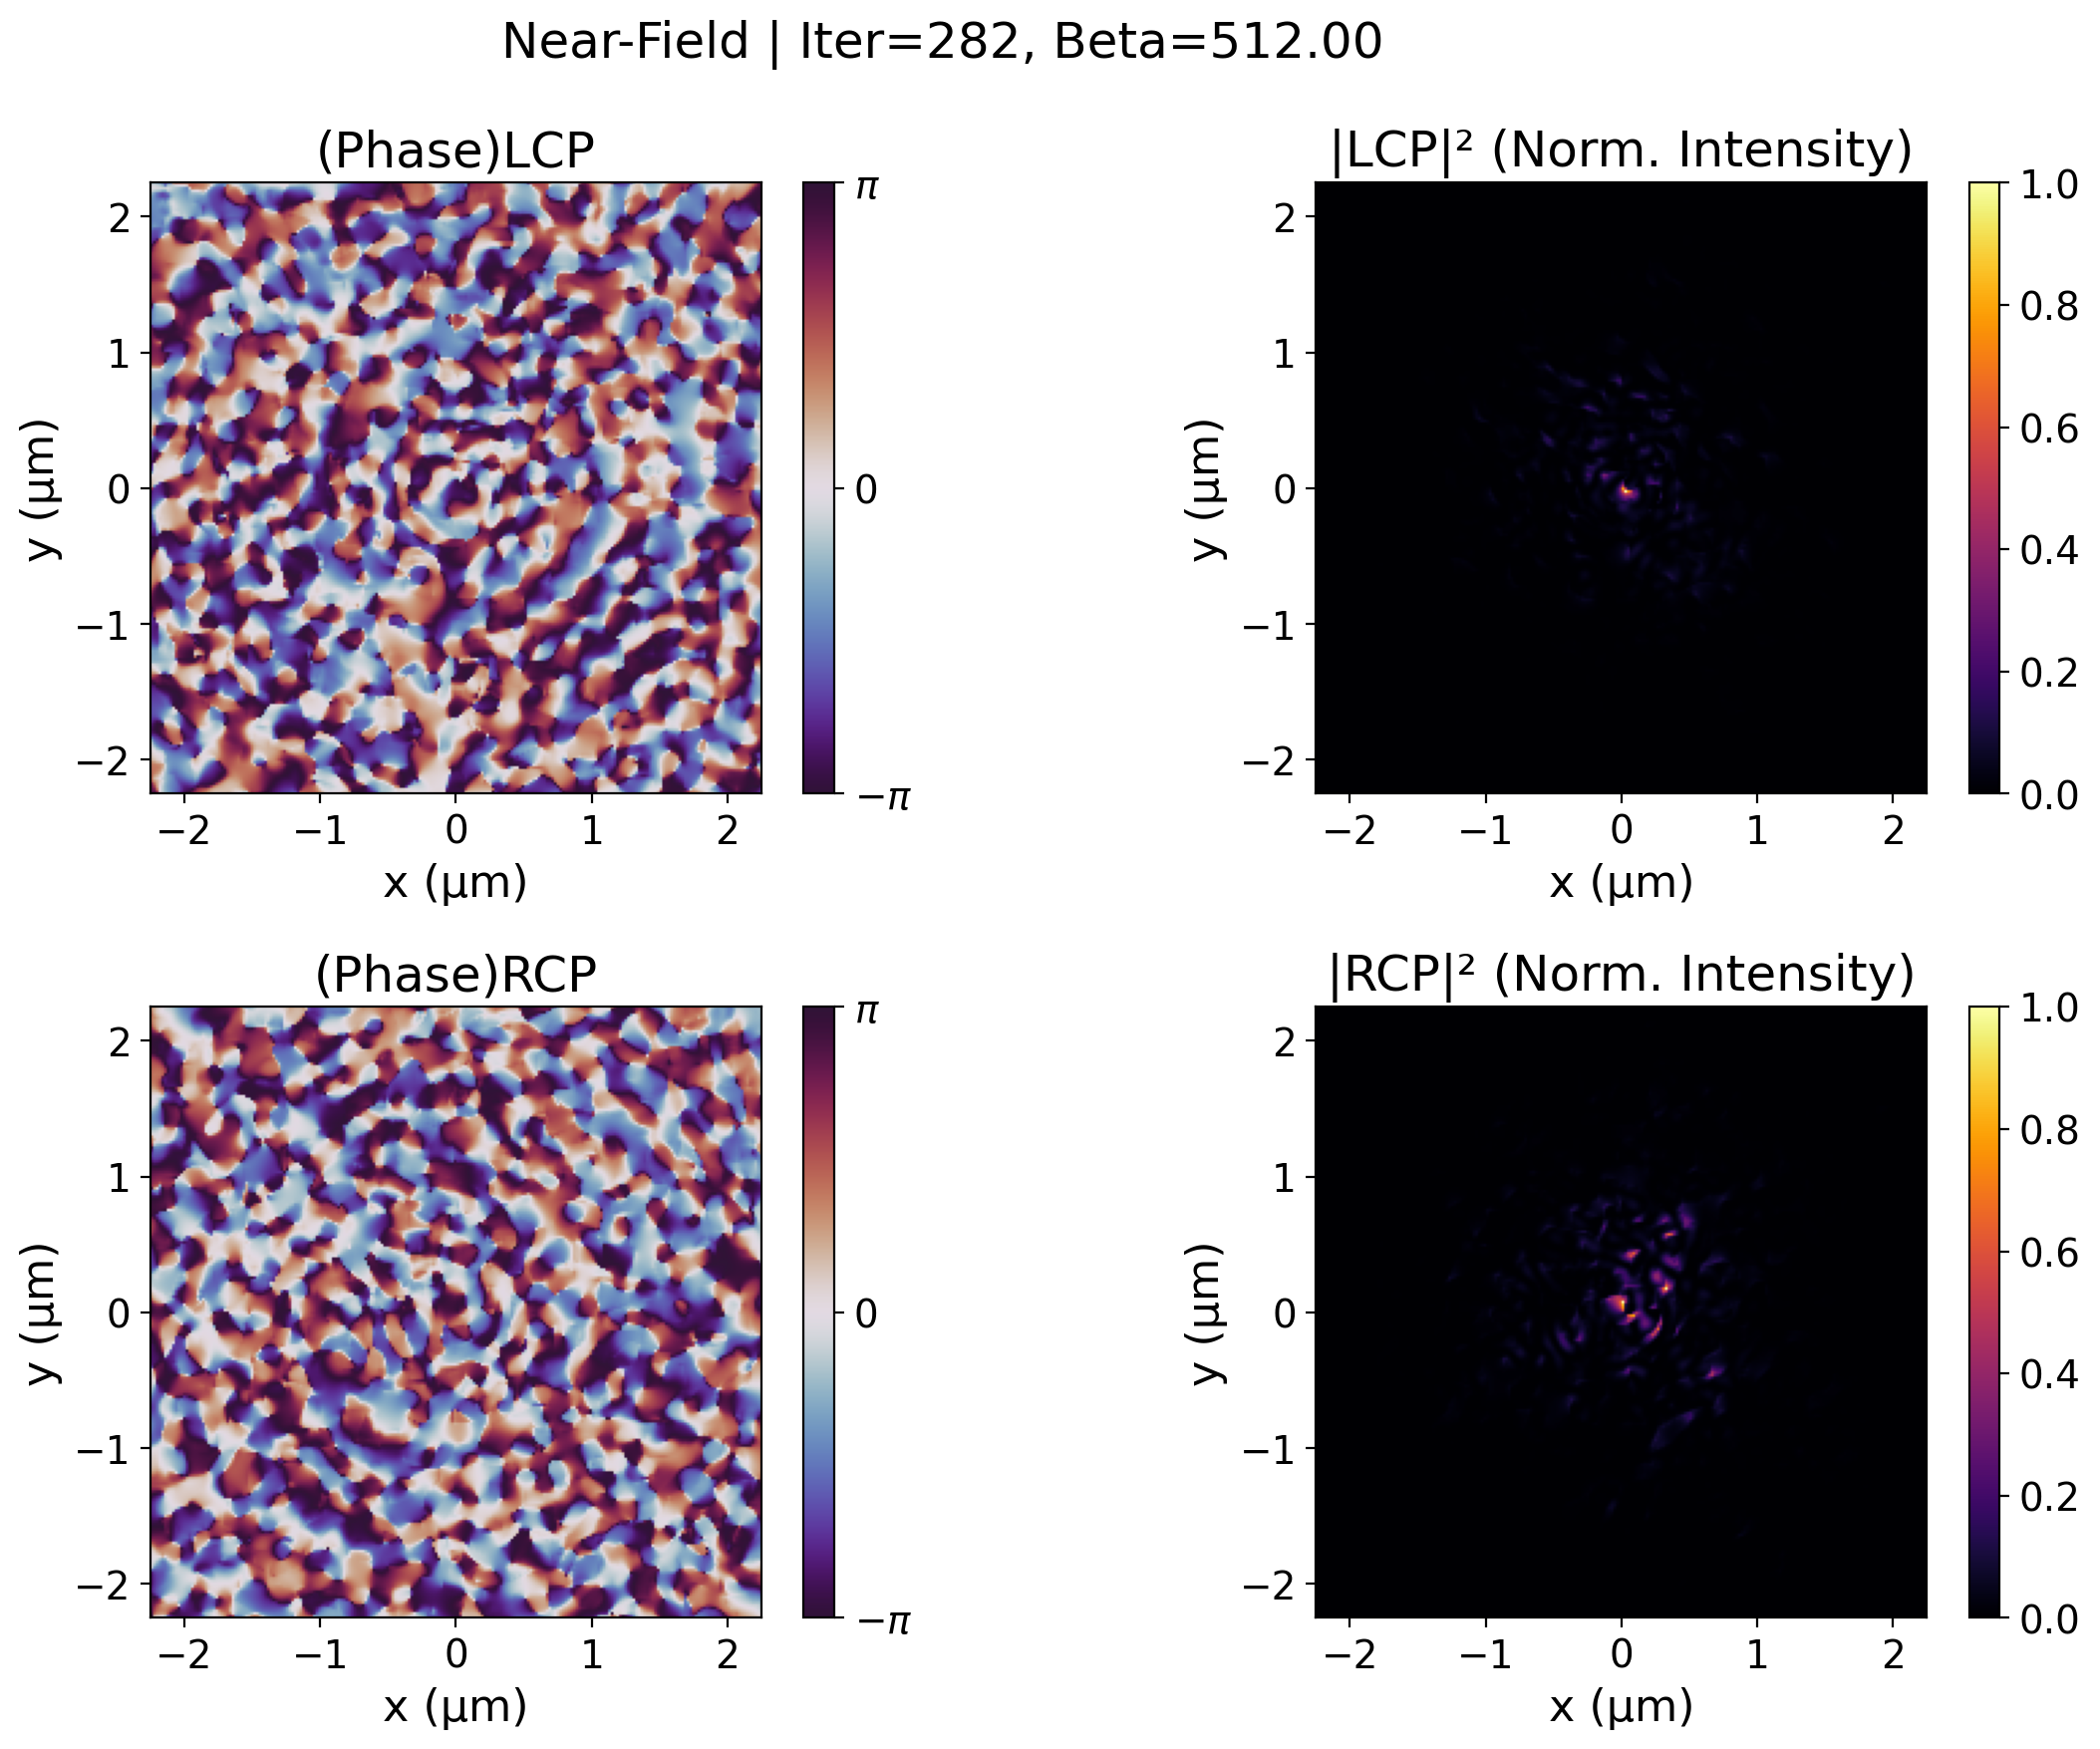
\includegraphics[width=0.47\textwidth]{img/020_phase_iter_282_beta_512.00.png}
	    \\  (c)  & (d) \\[6pt]
	    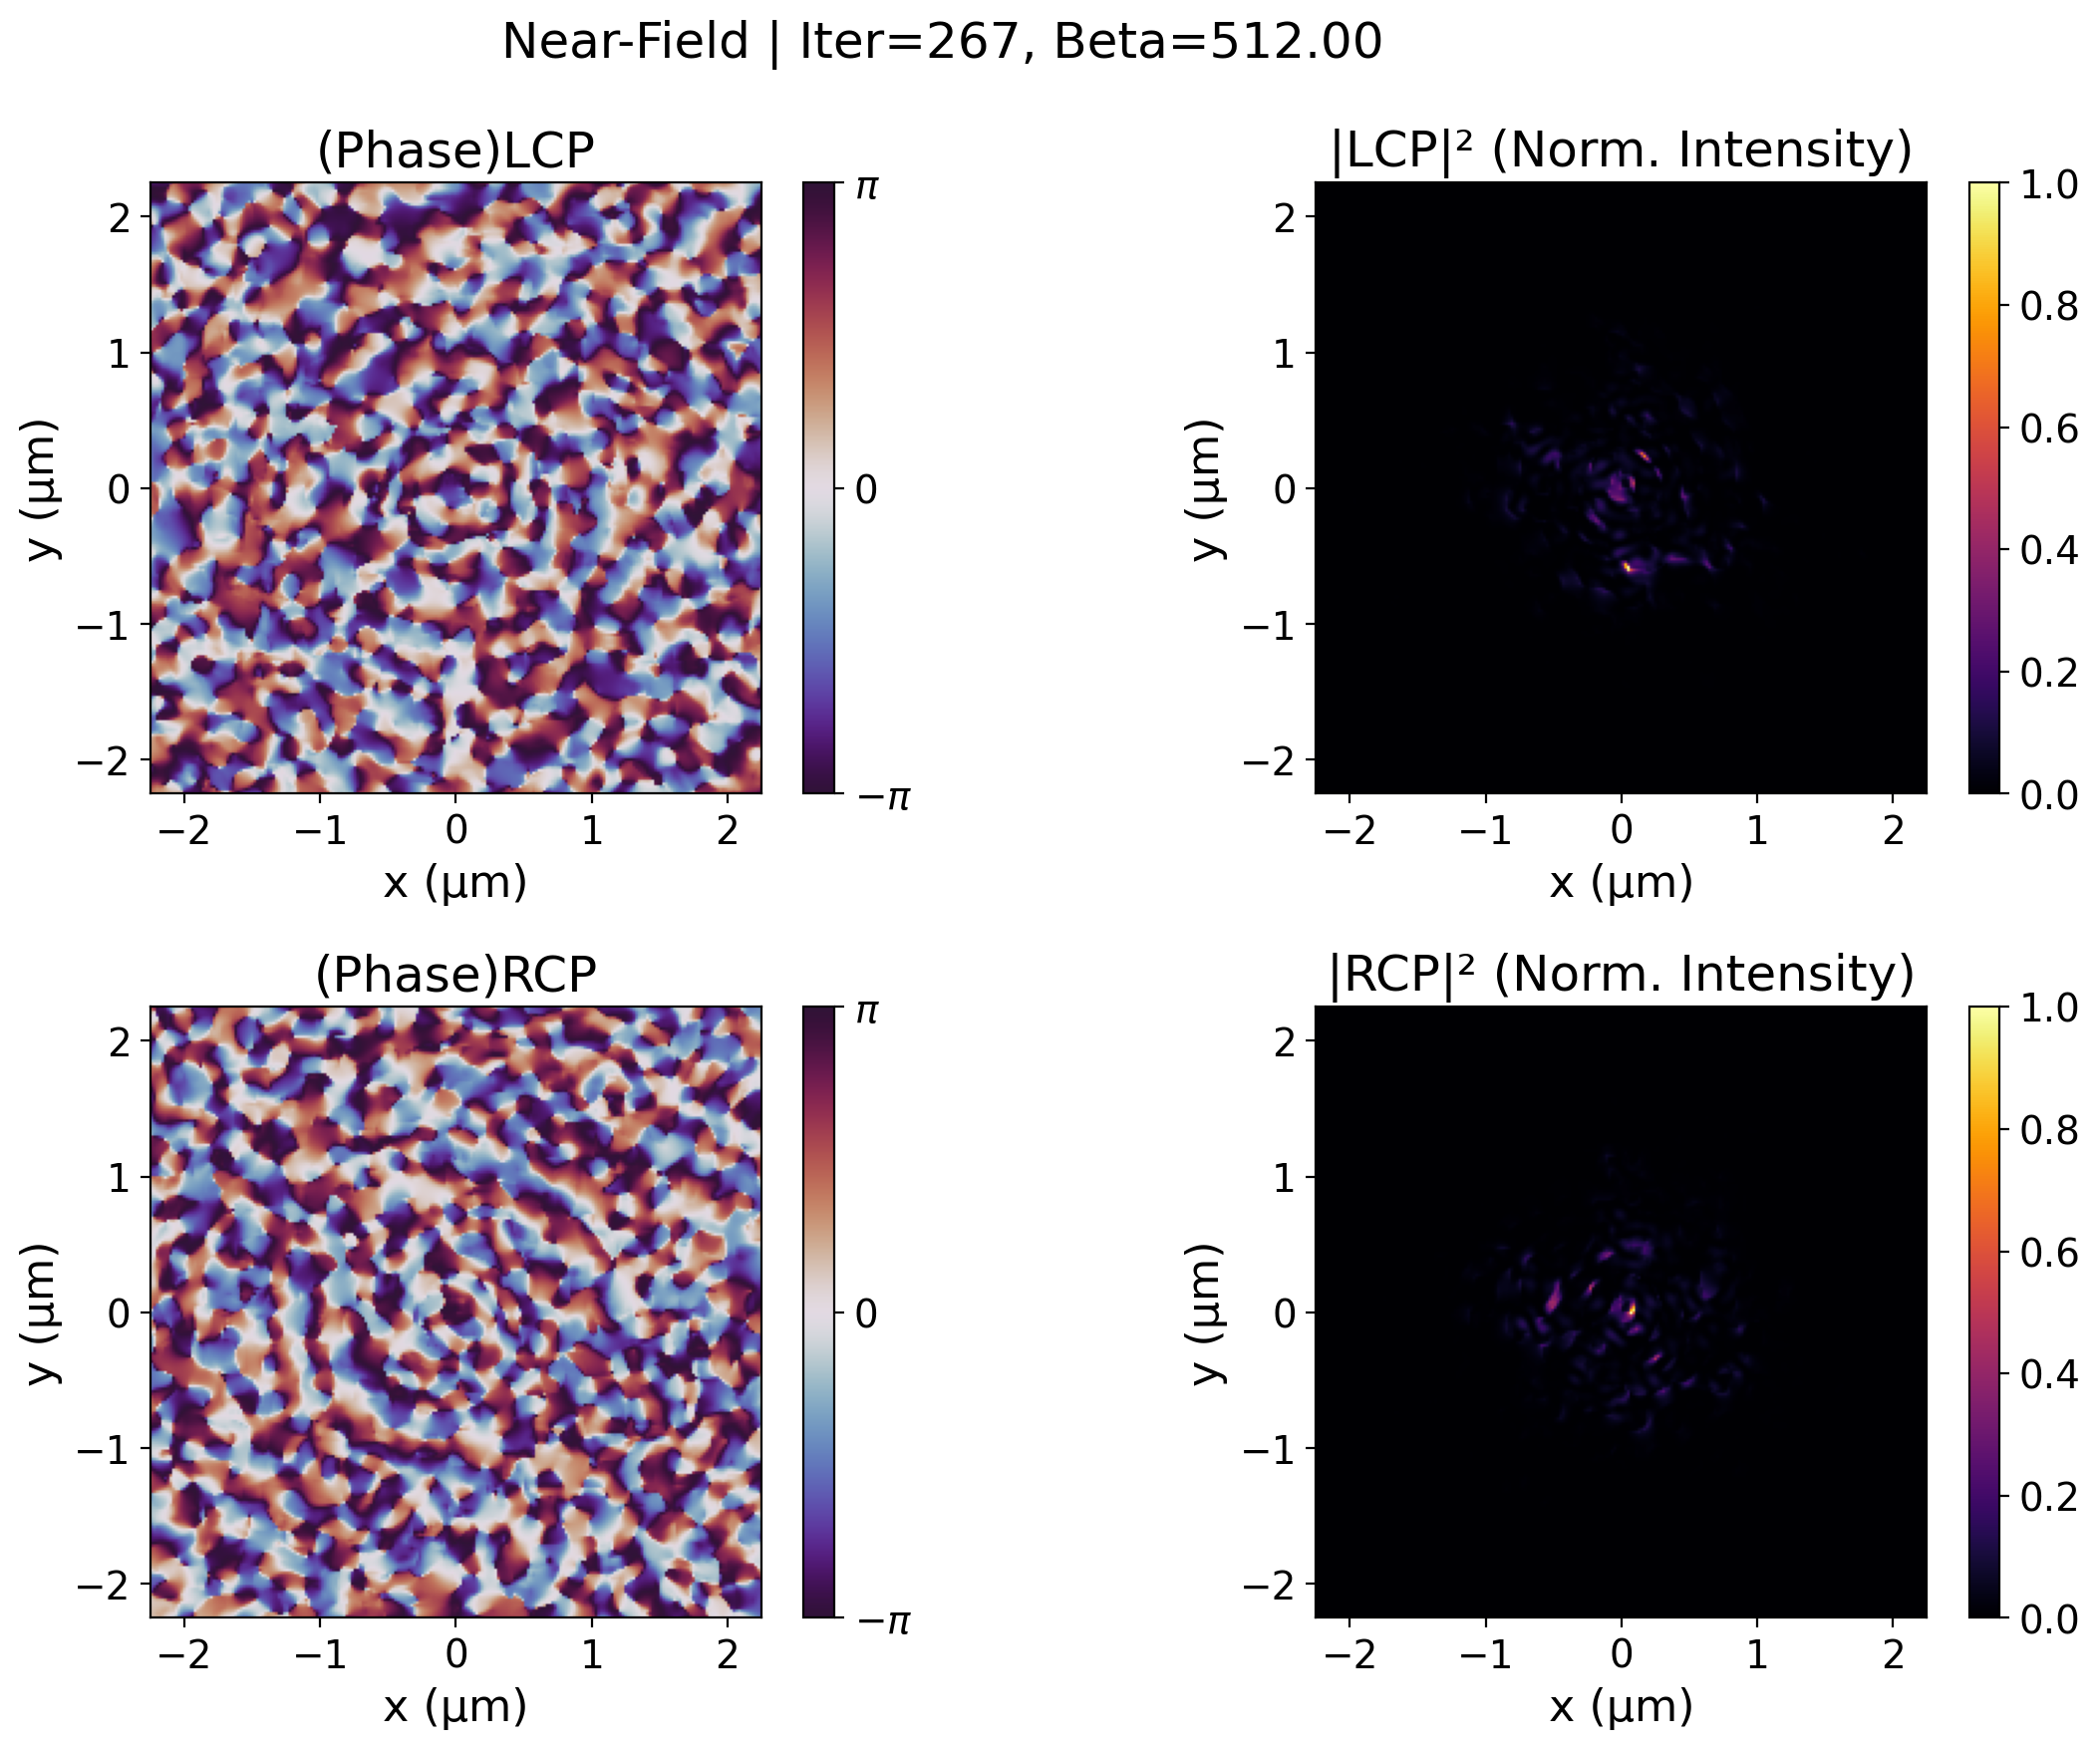
\includegraphics[width=0.47\textwidth]{img/021_phase_iter_267_beta_512.00.png}&
	    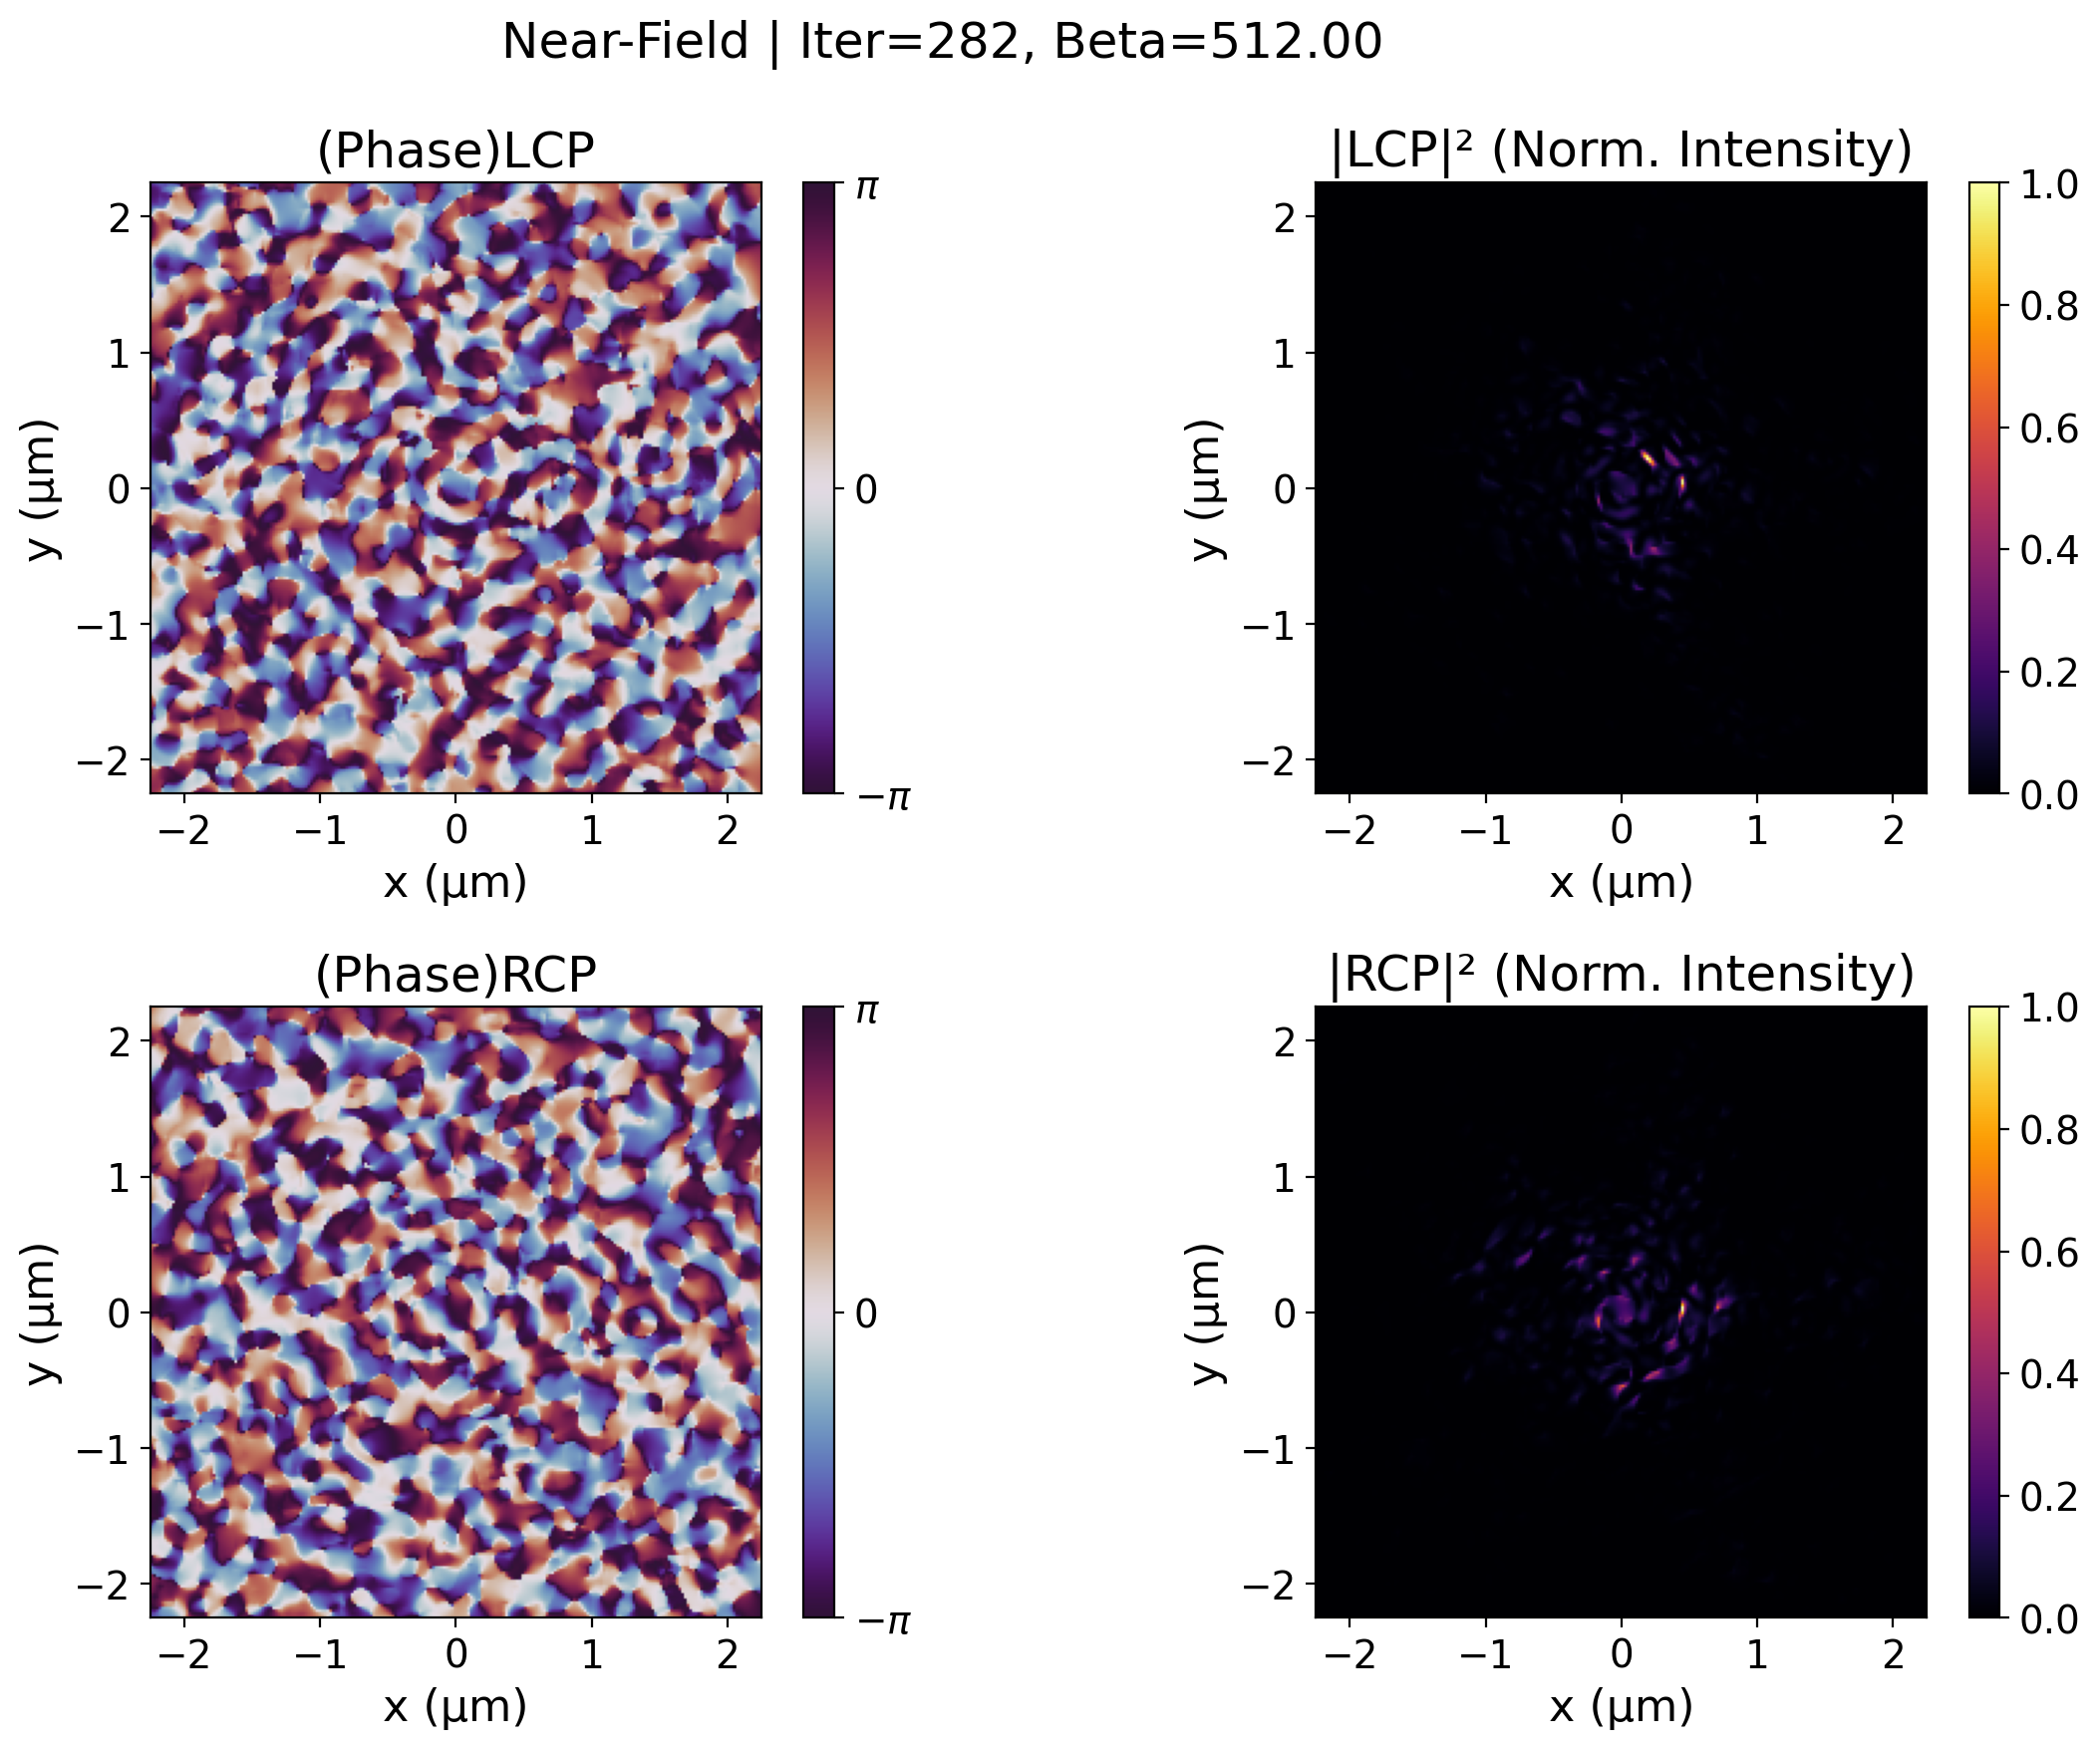
\includegraphics[width=0.47\textwidth]{img/022_phase_iter_282_beta_512.00.png}
	    \\ (e) & (f) 
	\end{tabular}
\caption{Near-field electric field distributions just above the design layer: (a)$\sim$(f) $\ell \in \{0, 1, 2, 3, 4, 5\}$, respectively. Each group of four panels: upper left — LCP phase; upper right — $|\text{LCP}|^2$ normalized intensity; lower left — RCP phase; lower right — $|\text{RCP}|^2$ normalized intensity.}
\label{fig:nearfield_all}
\end{figure}


%===================================================================

  
\section{Far-Field LG Mode Performance}

\label{sec:farfield}

Figure~\ref{fig:farfield_all} compares, in four-panel format, the simulated LCP phase and intensity (top row) and the theoretical phase and intensity of the target LG$_{\ell,0}$ mode (bottom row) for all six designs at the far-field evaluation plane $z = 10\,z_R$.

\textbf{Intensity distribution:} The $\ell = 0$ far field shows a Gaussian profile with a central intensity peak; all designs with $\ell \geq 1$ show a doughnut-shaped spot with zero center intensity, with the ring radius increasing with $\ell$, consistent with the LG mode theoretical prediction (peak radius $r_\text{peak} = w_0\sqrt{\ell/2}$). The ring spots for high topological charges $\ell = 4, 5$ are slightly uneven.

\textbf{Phase distribution:} The far-field phase for $\ell = 0$ to $2$ clearly shows the corresponding spiral structure. The number of spiral arms and their rotation direction match the target mode exactly, qualitatively confirming the correctness of the topological charge for each design (detailed quantitative verification in Section~\ref{sec:winding}). However, for high topological charges $\ell = 3$ to $5$, the spiral arms do not align as perfectly at the intensity center as in the low topological charge cases, and for $\ell = 4$ and $5$ the phase shows some irregularity. This deviation reflects the inherent difficulty of shaping high-order OAM modes within a finite design space.

\textbf{Quantitative results:} Purity and $|\text{Overlap}|^2$ for all six designs are listed in Table~\ref{tab:results_summary}. The overall trend shows that purity decreases as $\ell$ increases, remaining above $94\%$ for $\ell \leq 3$, and dropping to about $82\%$ for $\ell = 4, 5$. $|\text{Overlap}|^2$ drops significantly from $60.92$ at $\ell = 0$ to below $4.00$ for $\ell \geq 4$. Since the monitor area was dynamically adjusted based on the spot size for each topological charge to ensure a fixed coverage ratio, this sharp drop does not arise from geometric truncation. Notably, despite $\ell = 2$ achieving the highest LG modal purity among all non-Gaussian designs, its $|\text{Overlap}|^2$ value ($7.99$) is lower than that of $\ell = 3$ ($18.69$), revealing a non-monotonic dependence that is not governed solely by the finite design domain. The physical mechanisms behind both observations are discussed in Section~\ref{ssec:purity_overlap}.
\begin{figure}[htb]
\centering
	\begin{tabular}{cc} 
	    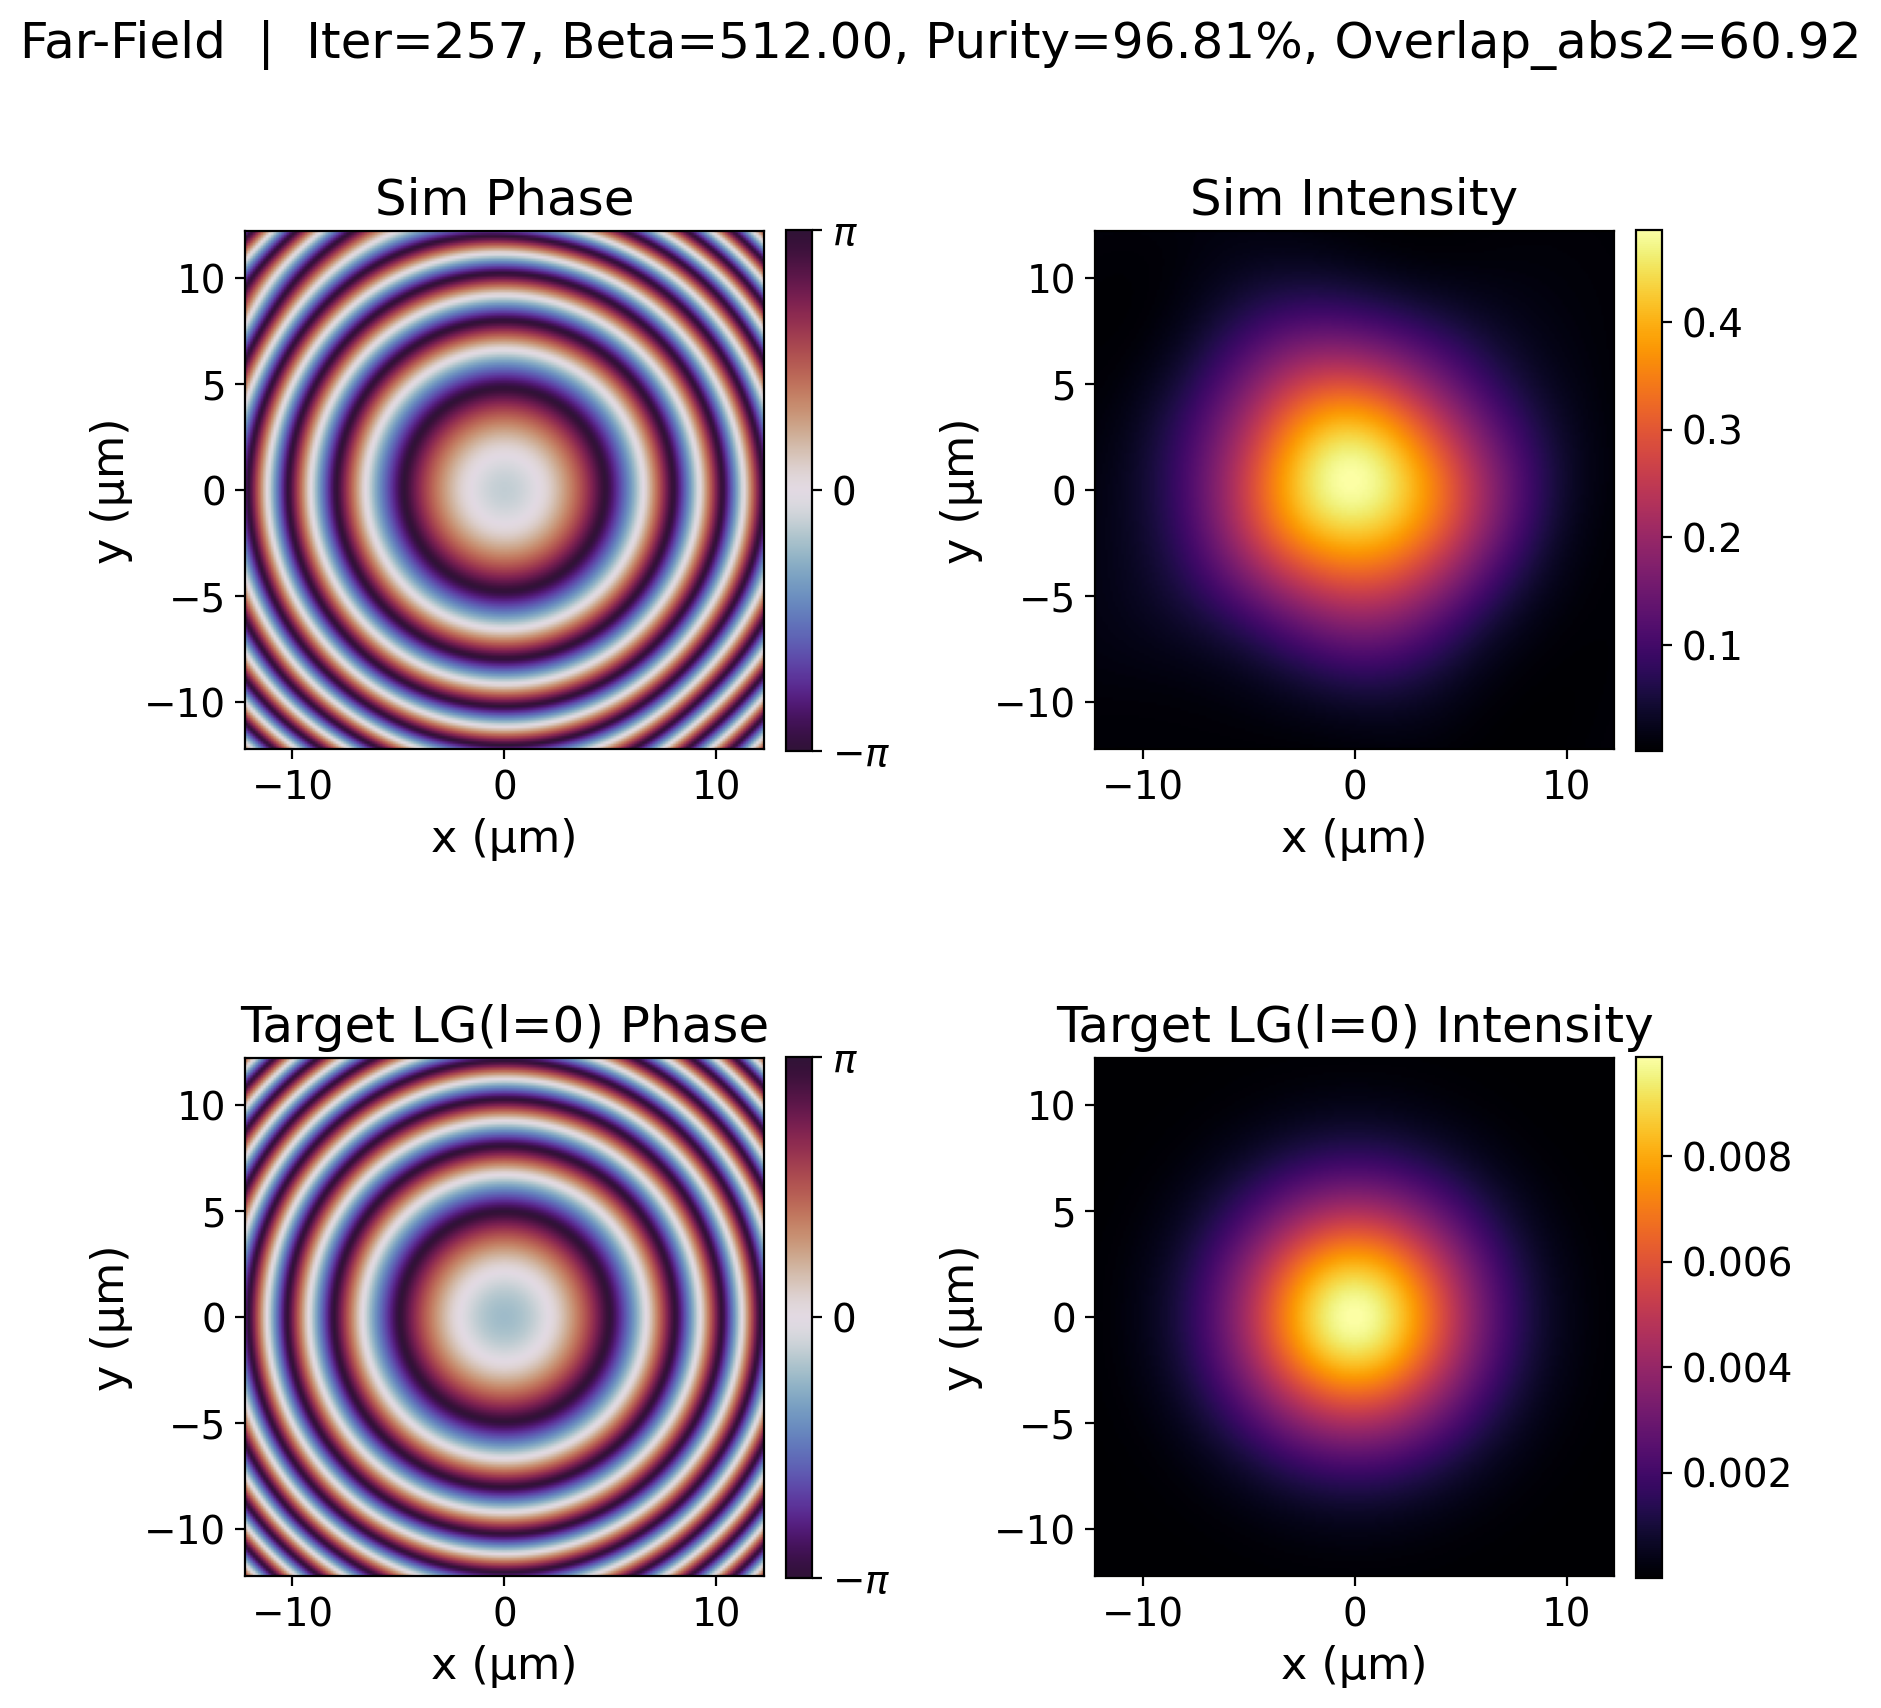
\includegraphics[width=0.47\textwidth]{img/017_ff_iter_257_beta_512.00.png}&
	    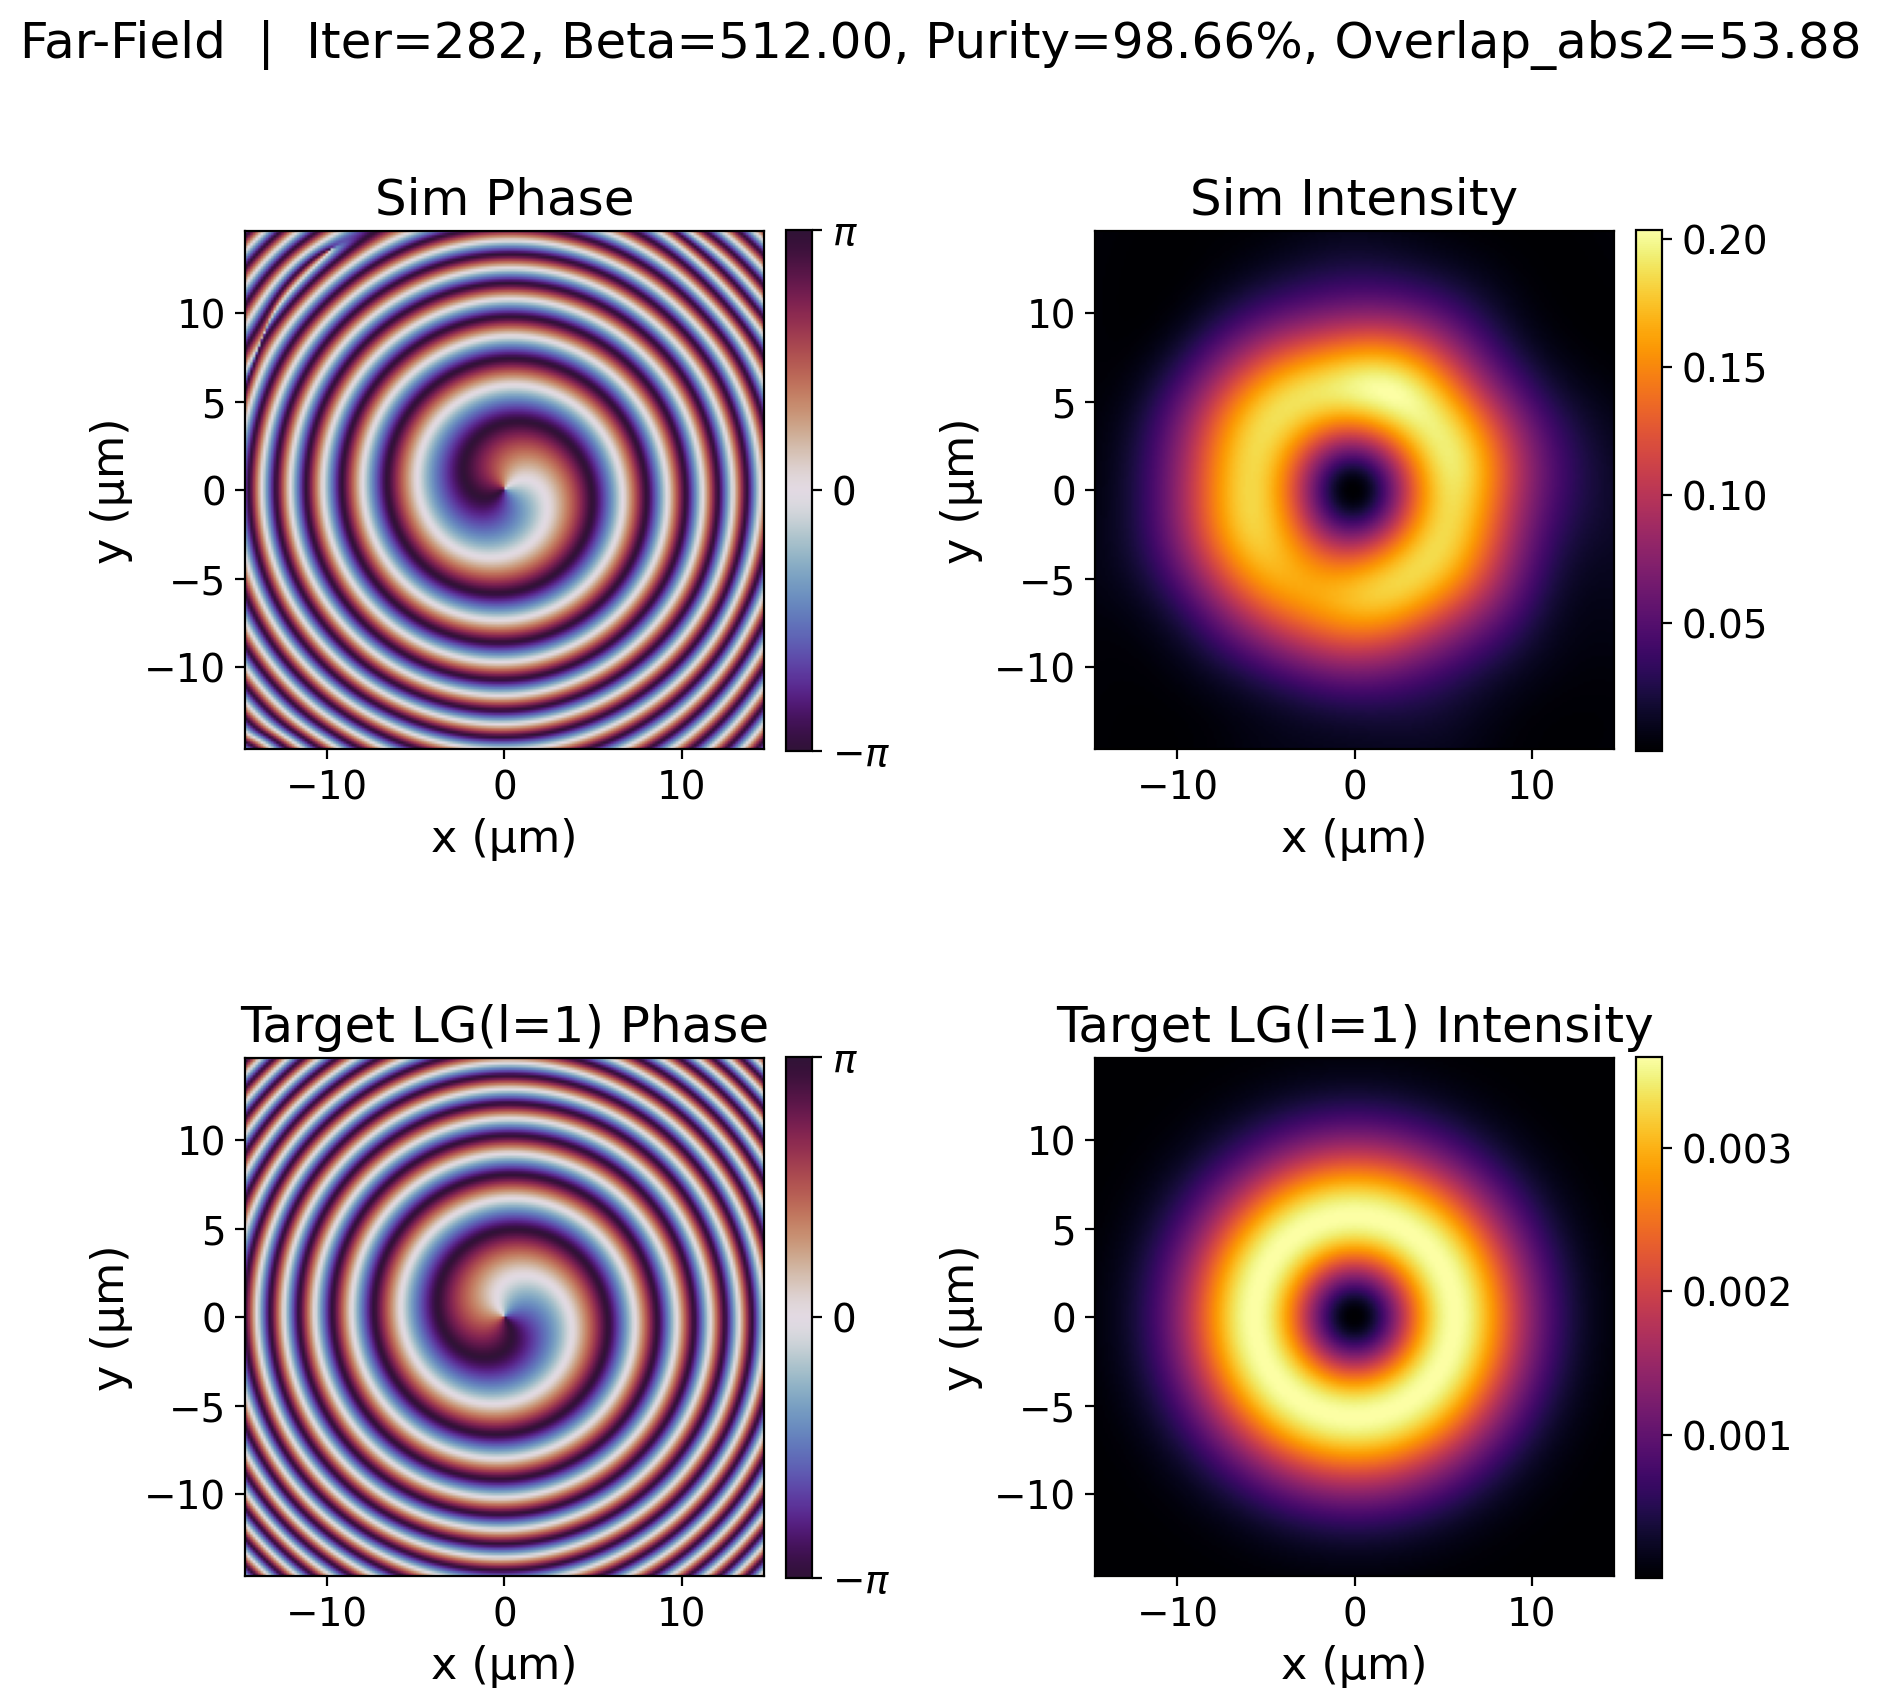
\includegraphics[width=0.47\textwidth]{img/018_ff_iter_282_beta_512.00.png}
		\\ (a) & (b)\\[6pt]
		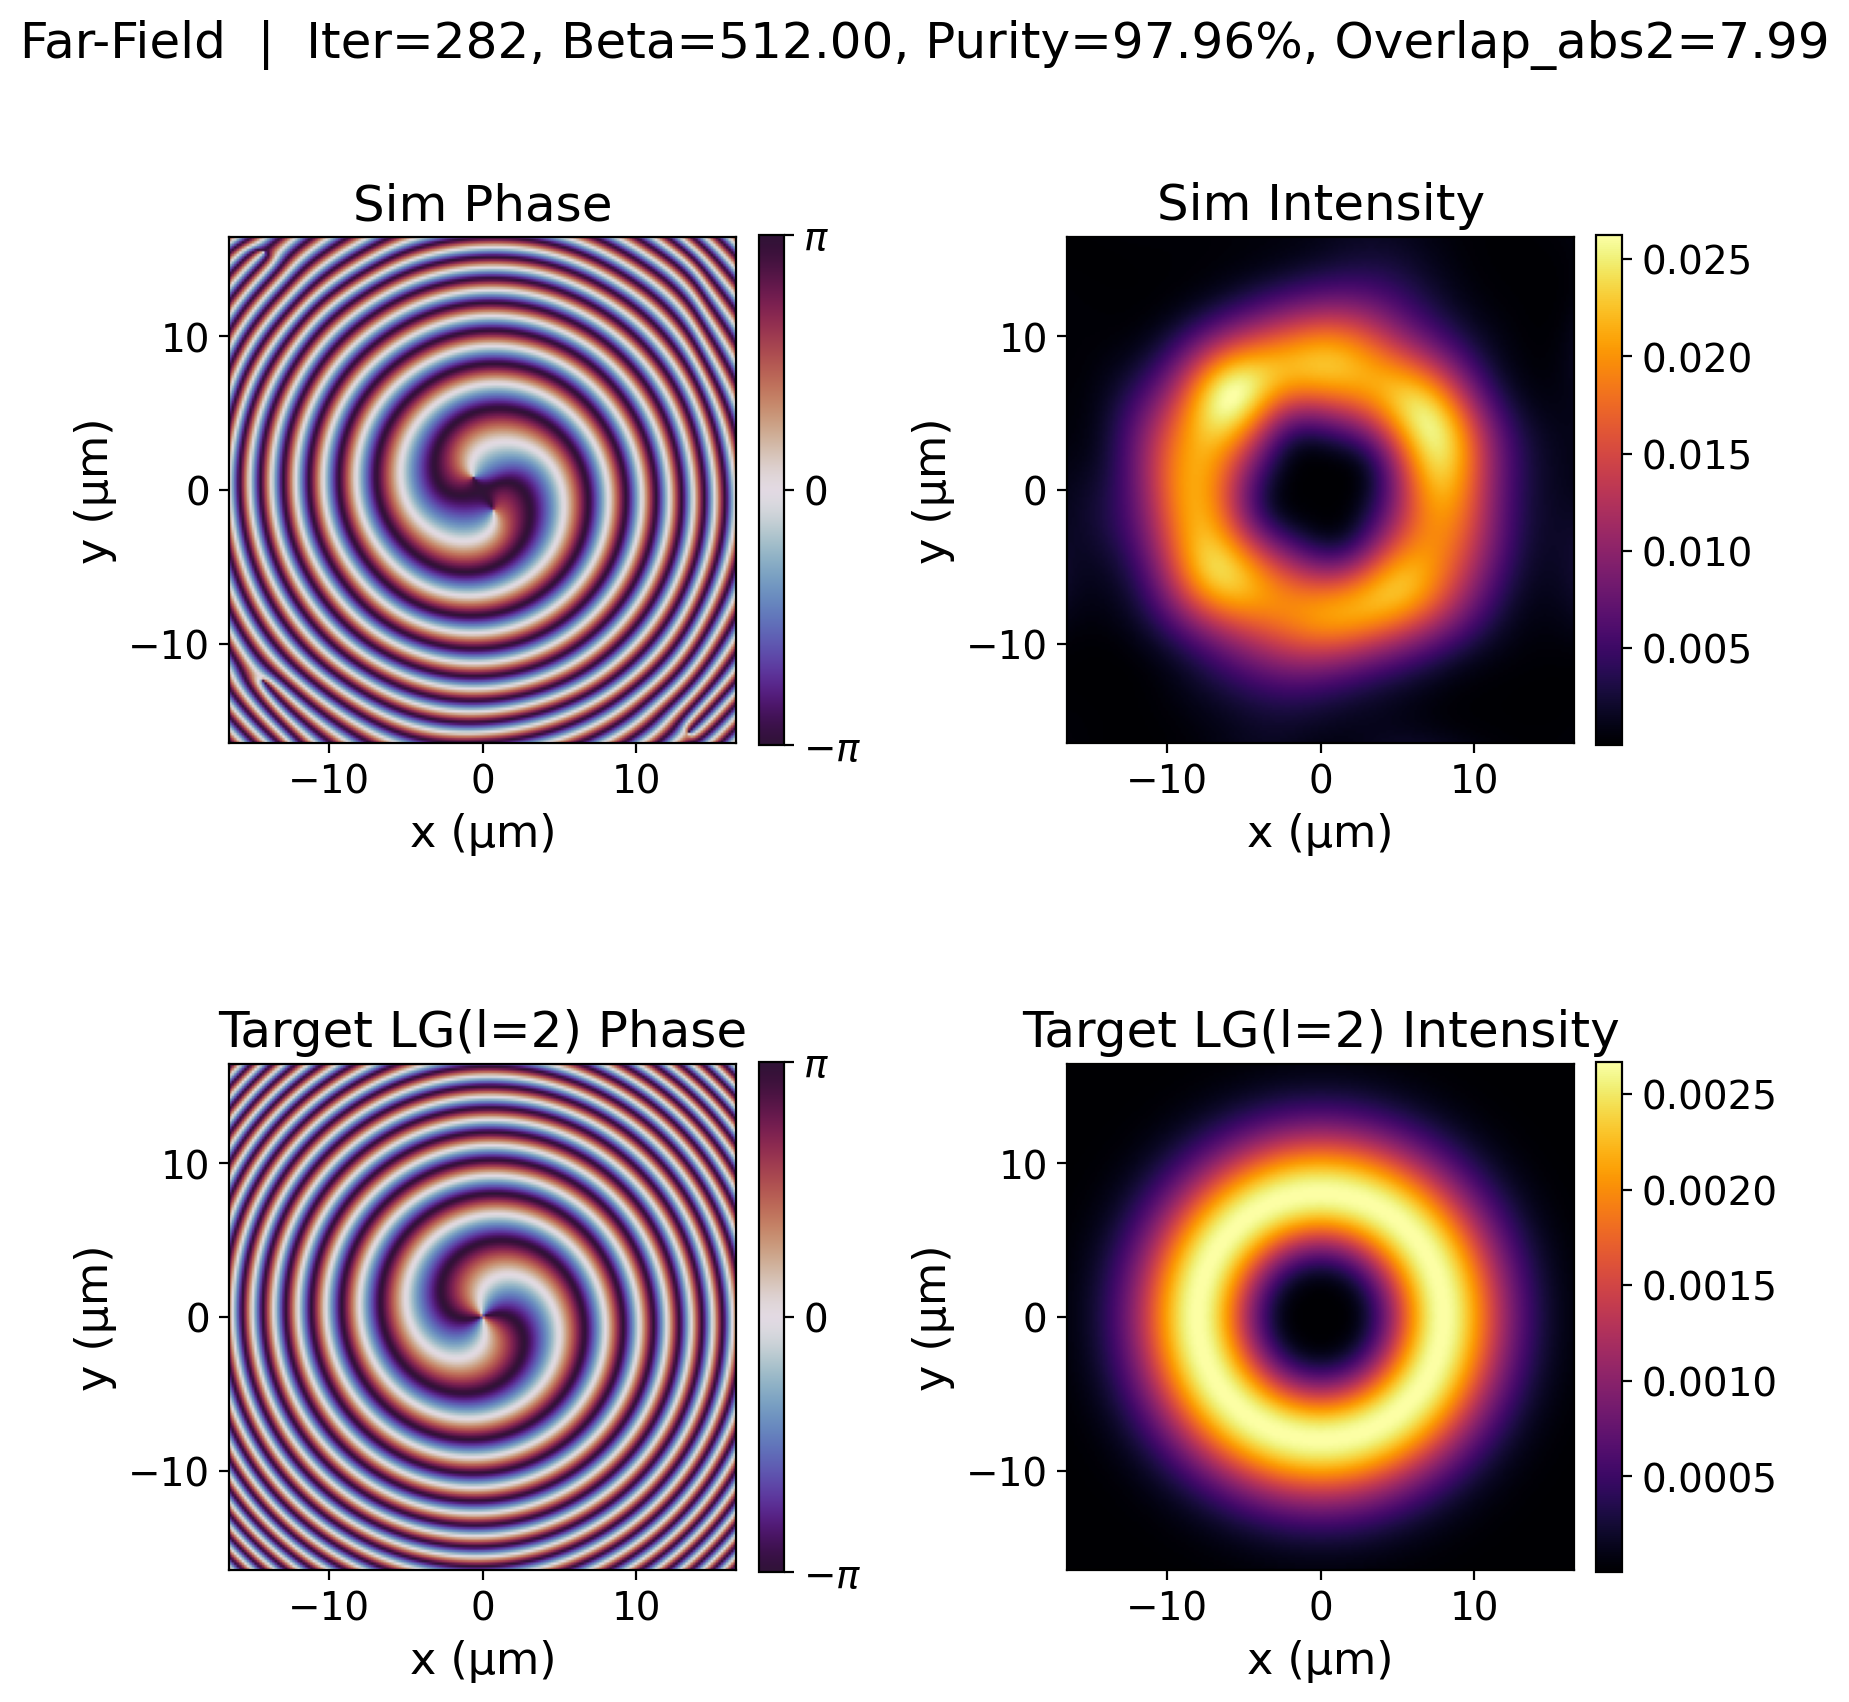
\includegraphics[width=0.47\textwidth]{img/013_ff_iter_282_beta_512.00.png}&
	    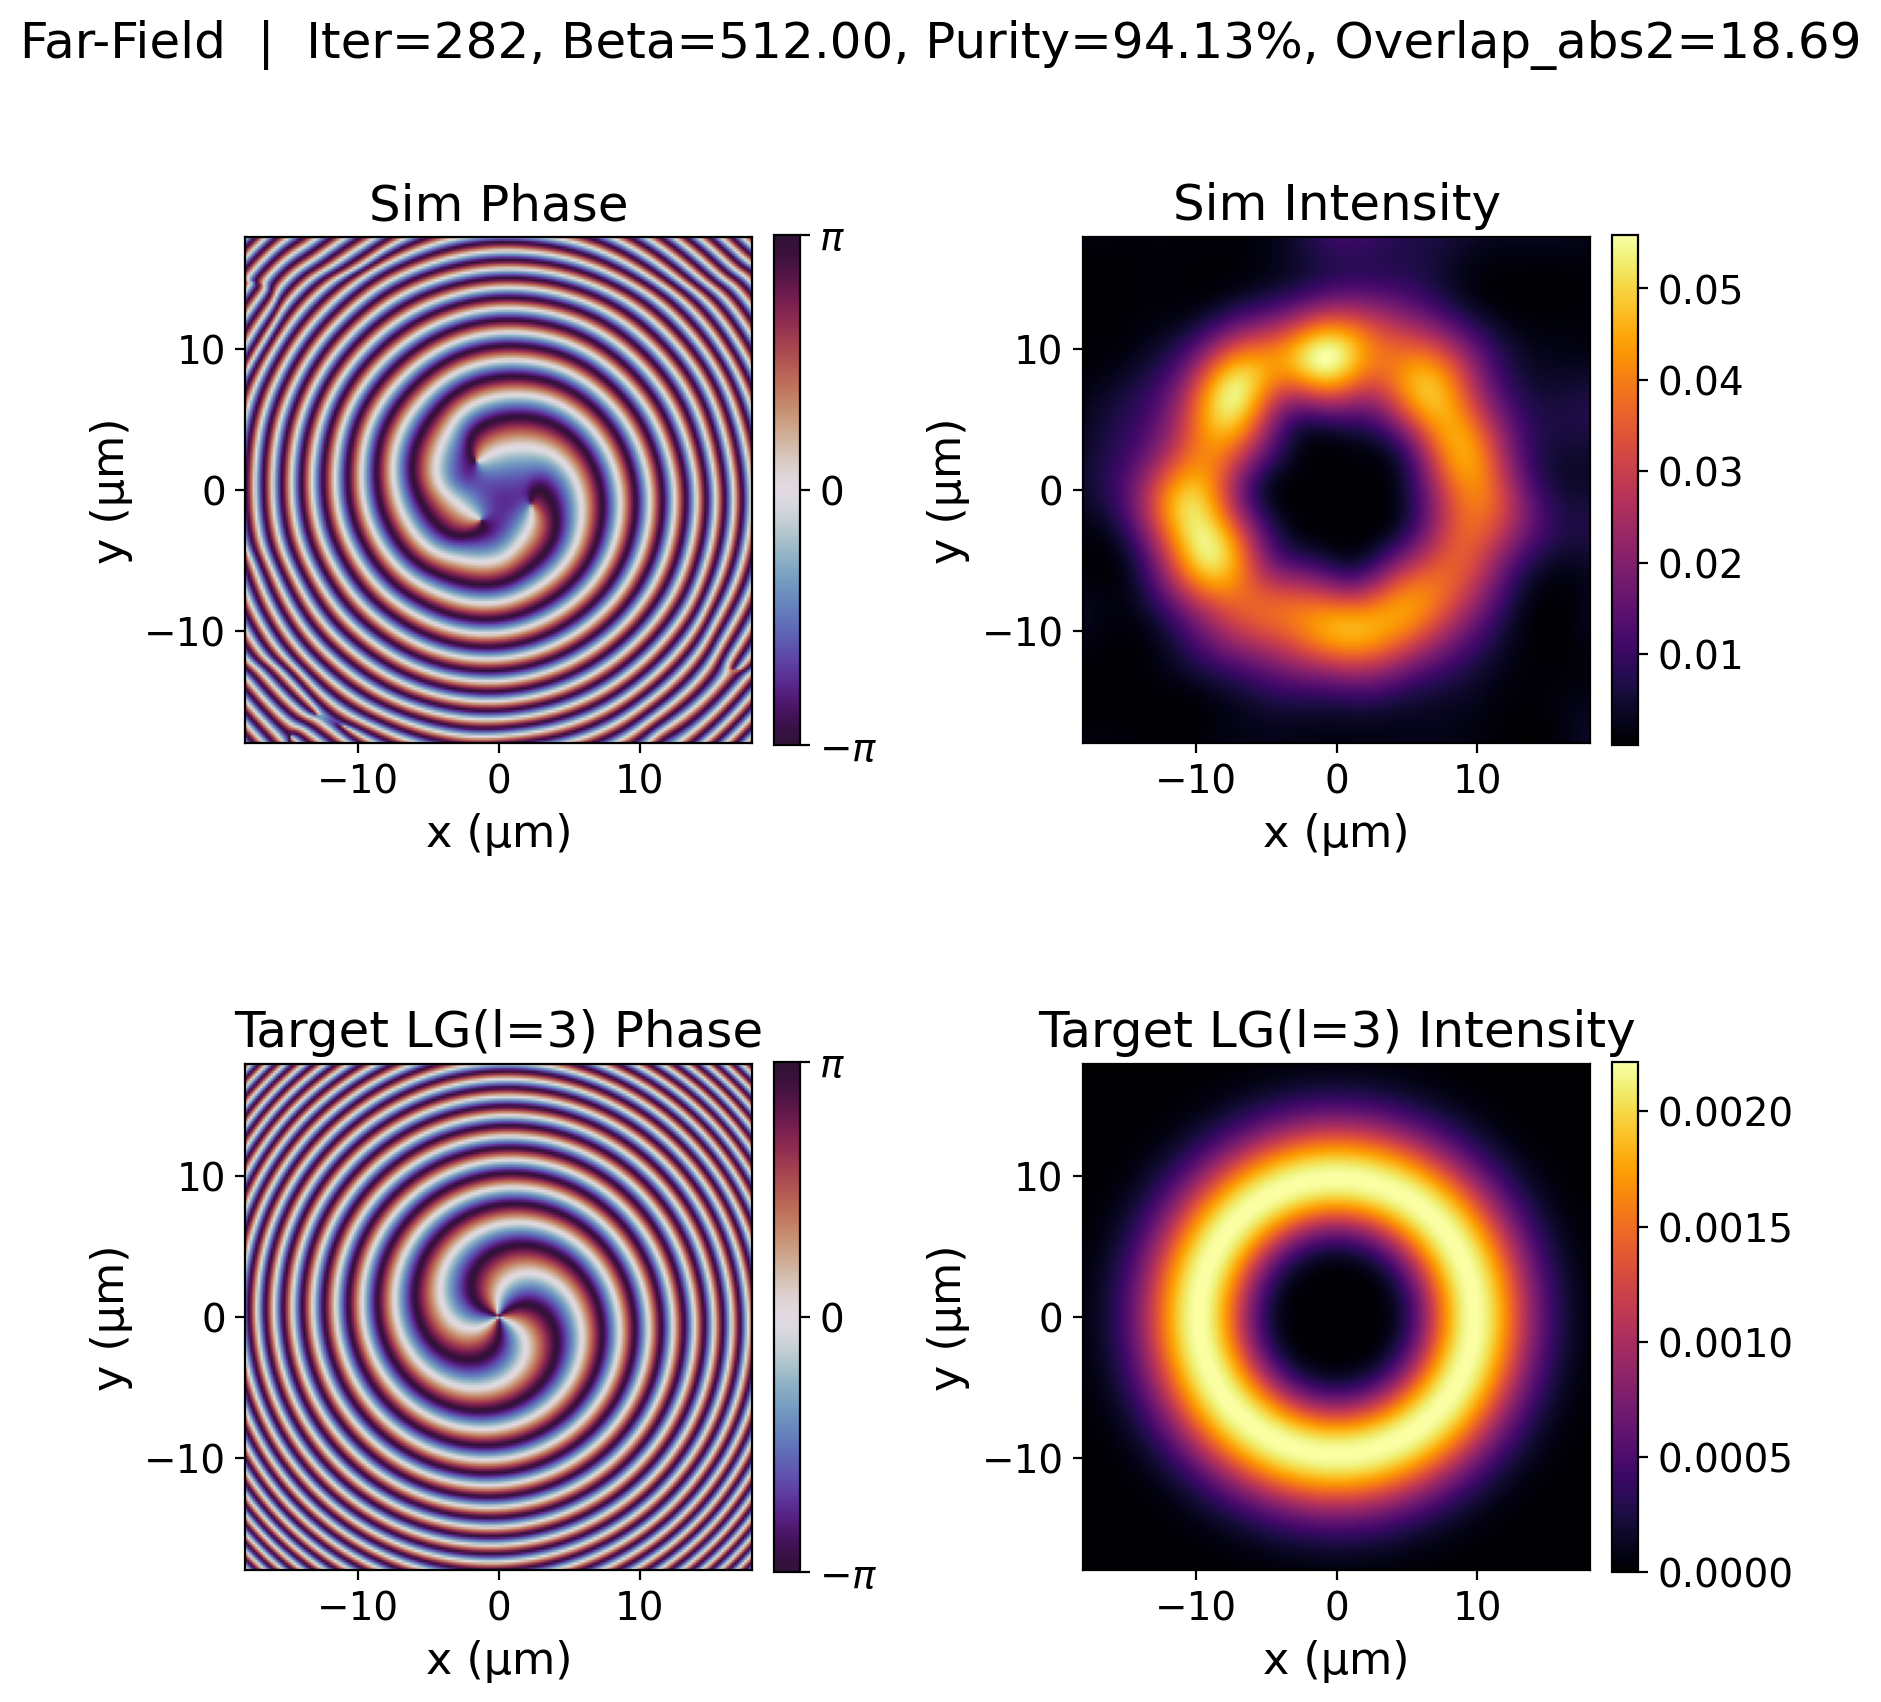
\includegraphics[width=0.47\textwidth]{img/020_ff_iter_282_beta_512.00.png}
	    \\(c) & (d)\\[6pt]
	    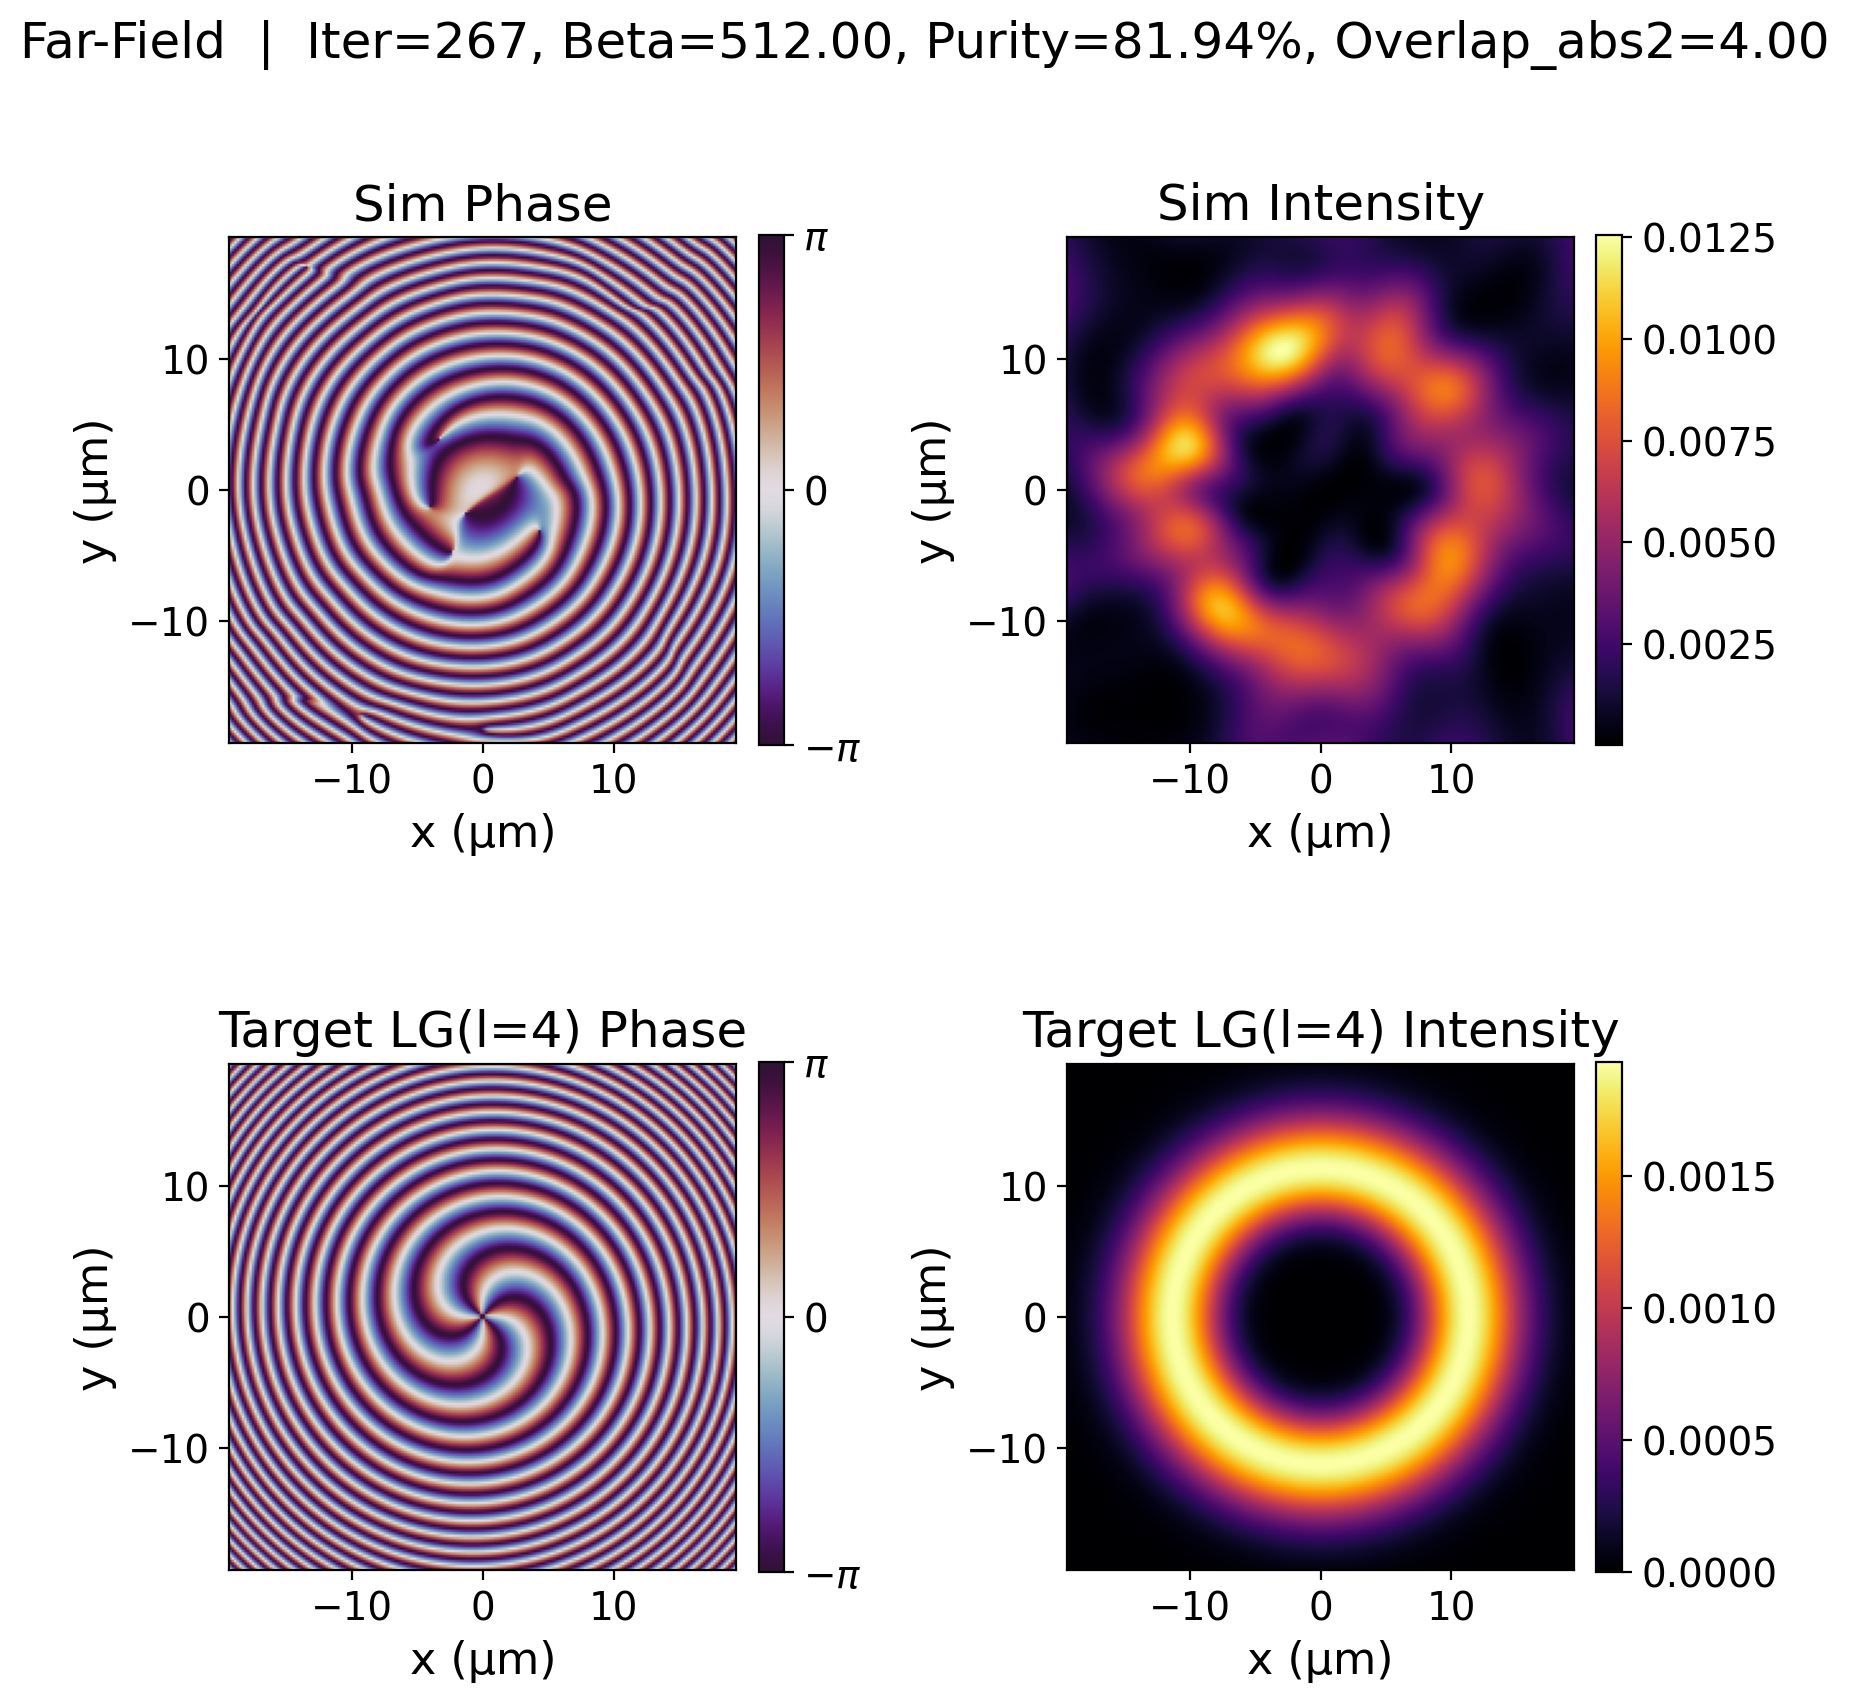
\includegraphics[width=0.47\textwidth]{img/021_ff_iter_267_beta_512.00.png}&
	    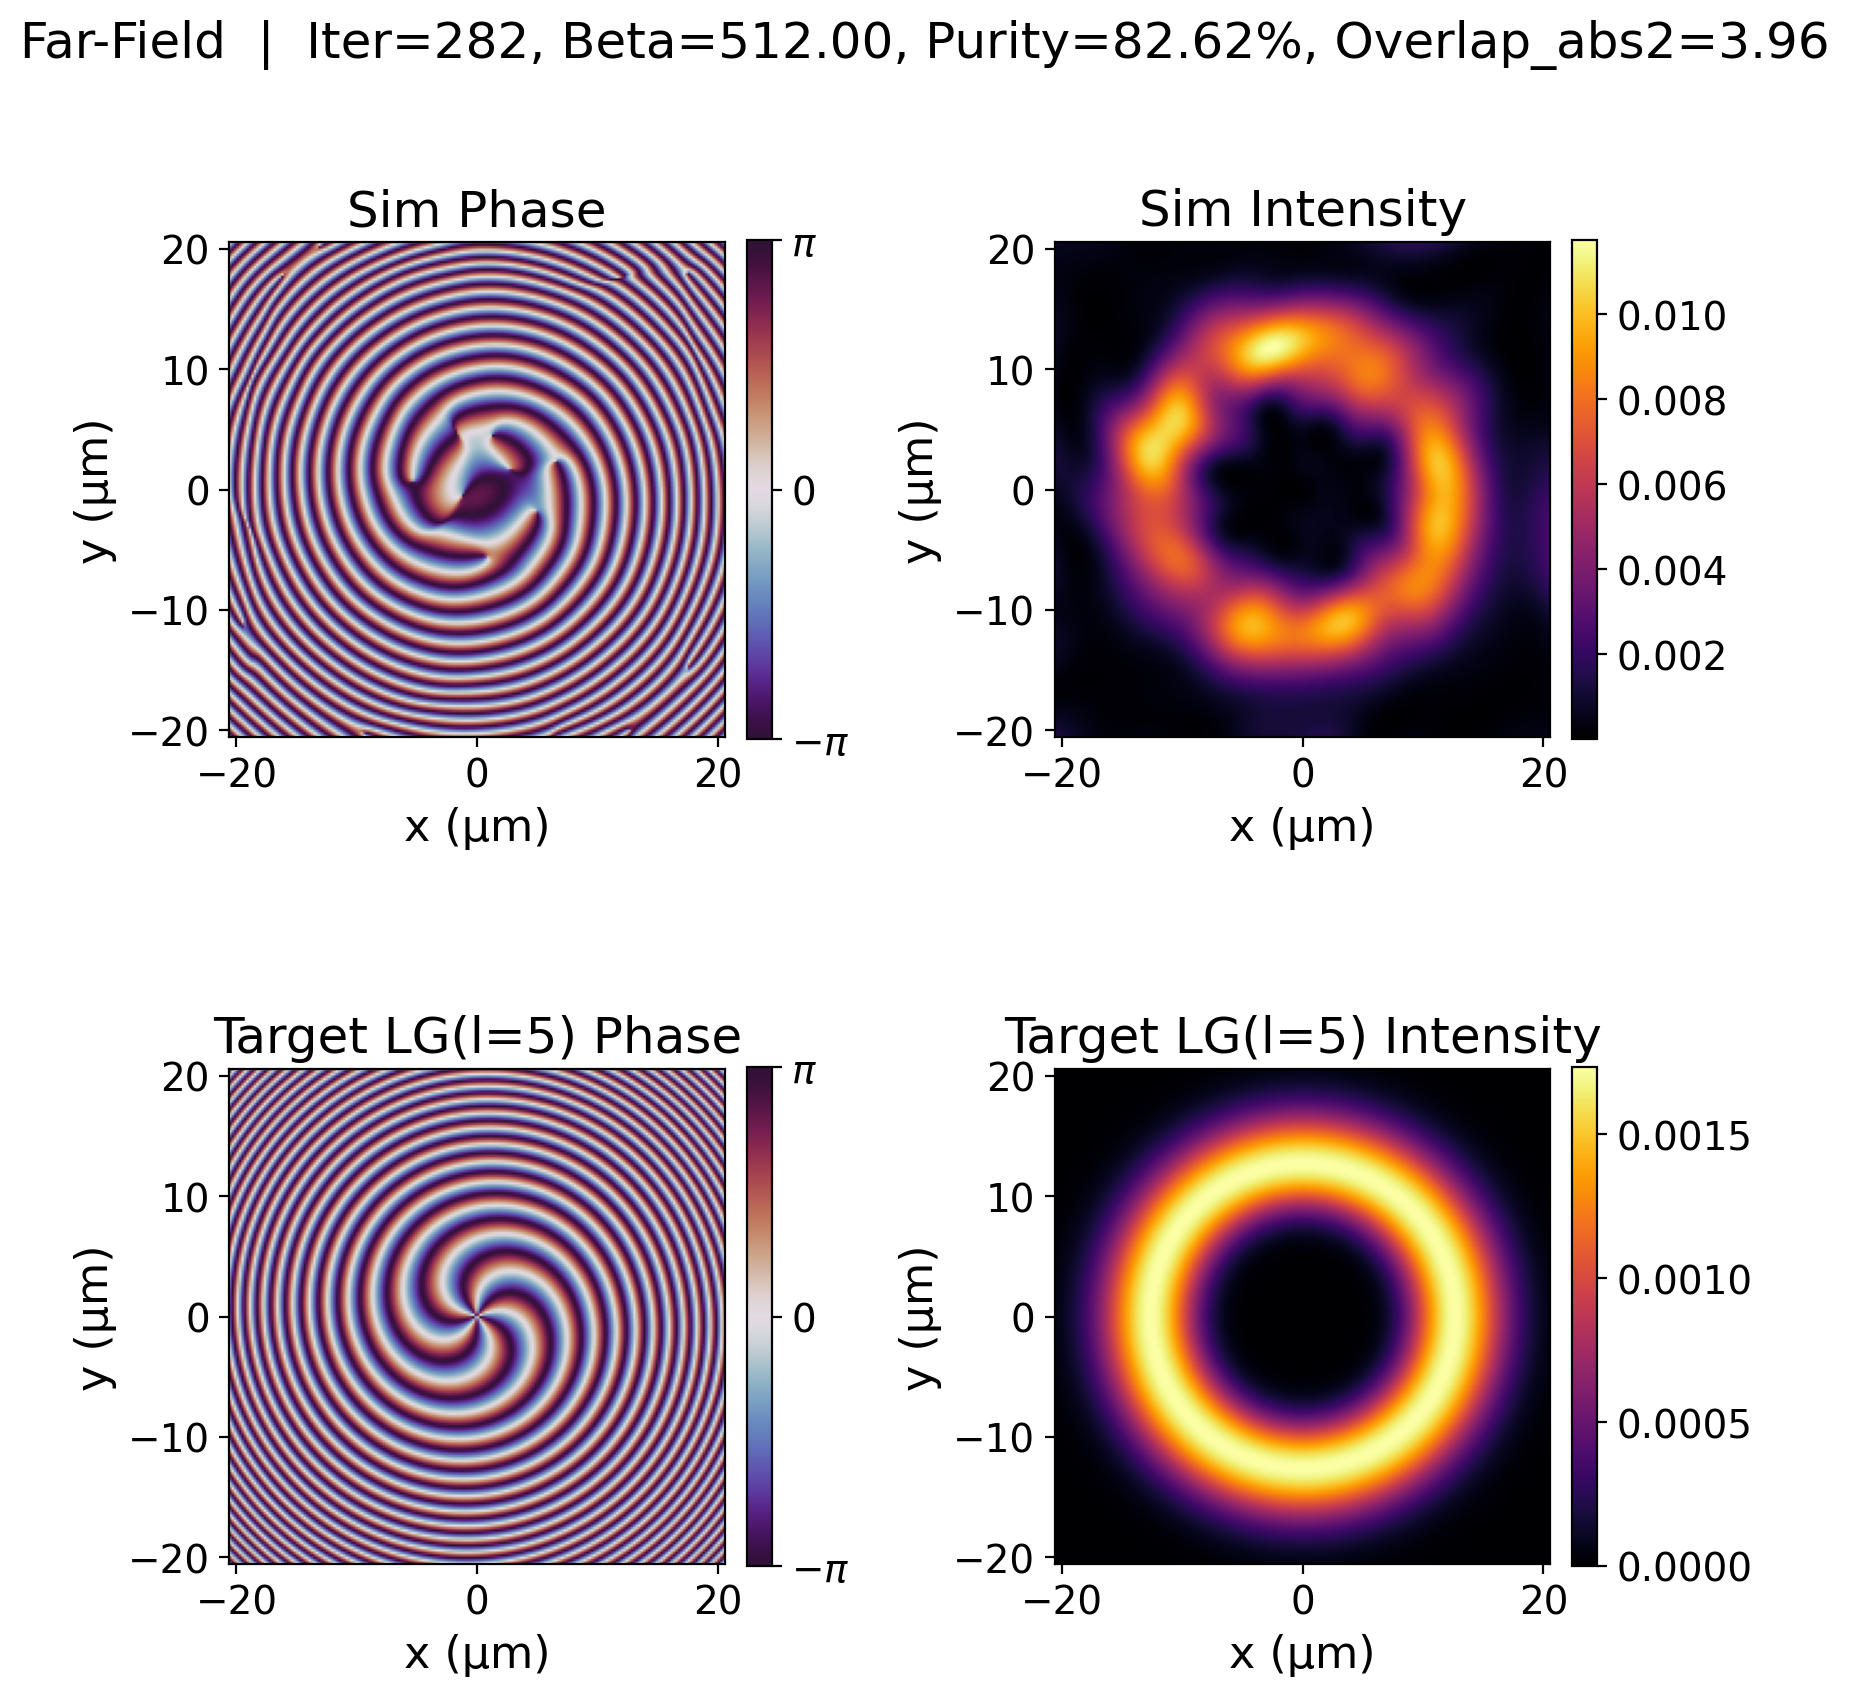
\includegraphics[width=0.47\textwidth]{img/022_ff_iter_282_beta_512.00.png}
	    \\(e) & (f)
	\end{tabular}
\caption{Far-field LG mode analysis ($z = 10\,z_R$): (a)$\sim$(f) $\ell \in \{0, 1, 2, 3, 4, 5\}$, respectively. Each group of four panels: upper left — simulated LG$_{\ell,0}$ phase; upper right — simulated LG$_{\ell,0}$ intensity; lower left — target LG$_{\ell,0}$ phase; lower right — target LG$_{\ell,0}$ intensity. Purity and $|\text{Overlap}|^2$ values are indicated at the top of each group.}
\label{fig:farfield_all}
\end{figure}

%===================================================================


\section{Optical Chirality}
\label{sec:chirality}

The optical chirality density $C \propto -\omega\,\varepsilon_0\,\text{Im} (\mathbf{E}^* \cdot \mathbf{B})$ quantifies the chiral character of the electromagnetic field in space: $C > 0$ indicates RCP dominance; $C < 0$ indicates LCP dominance. This section first uses the high-order mode ($\ell = 5$) as a representative case to analyze how optical chirality evolves along the propagation axis ($z$-axis), and then compares the near-field and far-field chirality distributions across all six designs.

\subsection{Chirality Propagation}
\label{ssec:chirality_prop}
To clarify the physical mechanism of chirality evolution during beam propagation, Figure~\ref{fig:chirality_prop} shows cross-sections of the optical chirality density distribution for the $\ell = 5$ mode propagating from the near field ($z \approx 0^+$) to the far field ($z = 10\,z_R$).

The results show that the near-field region ($z \ll z_R$) displays a pronounced LCP/RCP mixed state, strongly influenced by the intense local scattering and evanescent wave coupling of the topological structure; a substantial fraction of the area above the point source shows blue positive values ($C > 0$), indicating local RCP-dominant components generated by near-field scattering from the nanostructure. However, as the propagation distance $z$ increases, the non-radiative evanescent waves decay exponentially and quickly vanish, and the local scattering field approaches zero; when the beam enters the far-field radiation region ($z \ge z_R$), it is completely dominated by the propagating field, and the optical chirality recovers to a pure and uniform LCP state ($C < 0$), consistent with the handedness of the K-valley LCP source. This evolution fully confirms that the far-field propagating field perfectly preserves the LCP chirality of the source.

\begin{figure}[htb]
\centering
    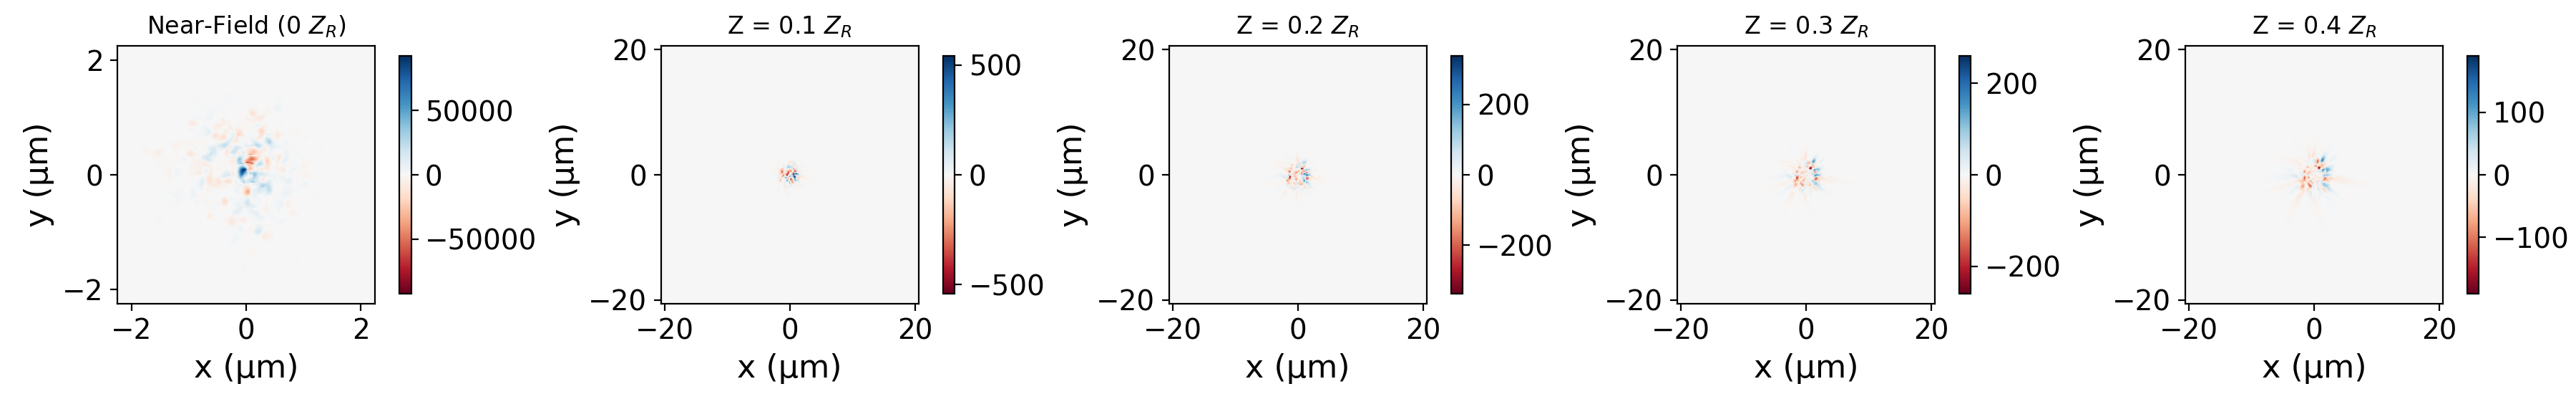
\includegraphics[width=1.0\textwidth]{img/chirality_prop_0p0to0p9zr_Fixed_XY_360_1.png}\\[2pt]
    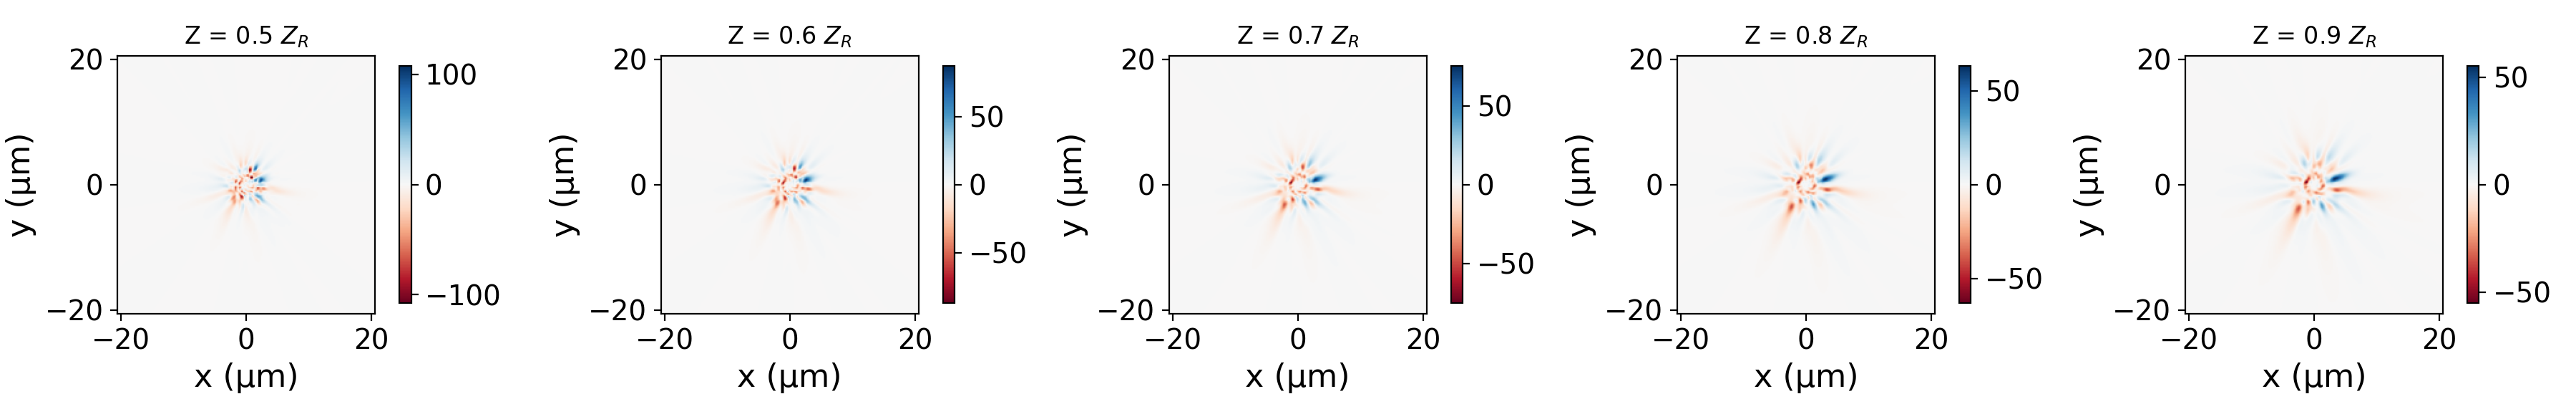
\includegraphics[width=1.0\textwidth]{img/chirality_prop_0p0to0p9zr_Fixed_XY_360_2.png}\\[4pt]
    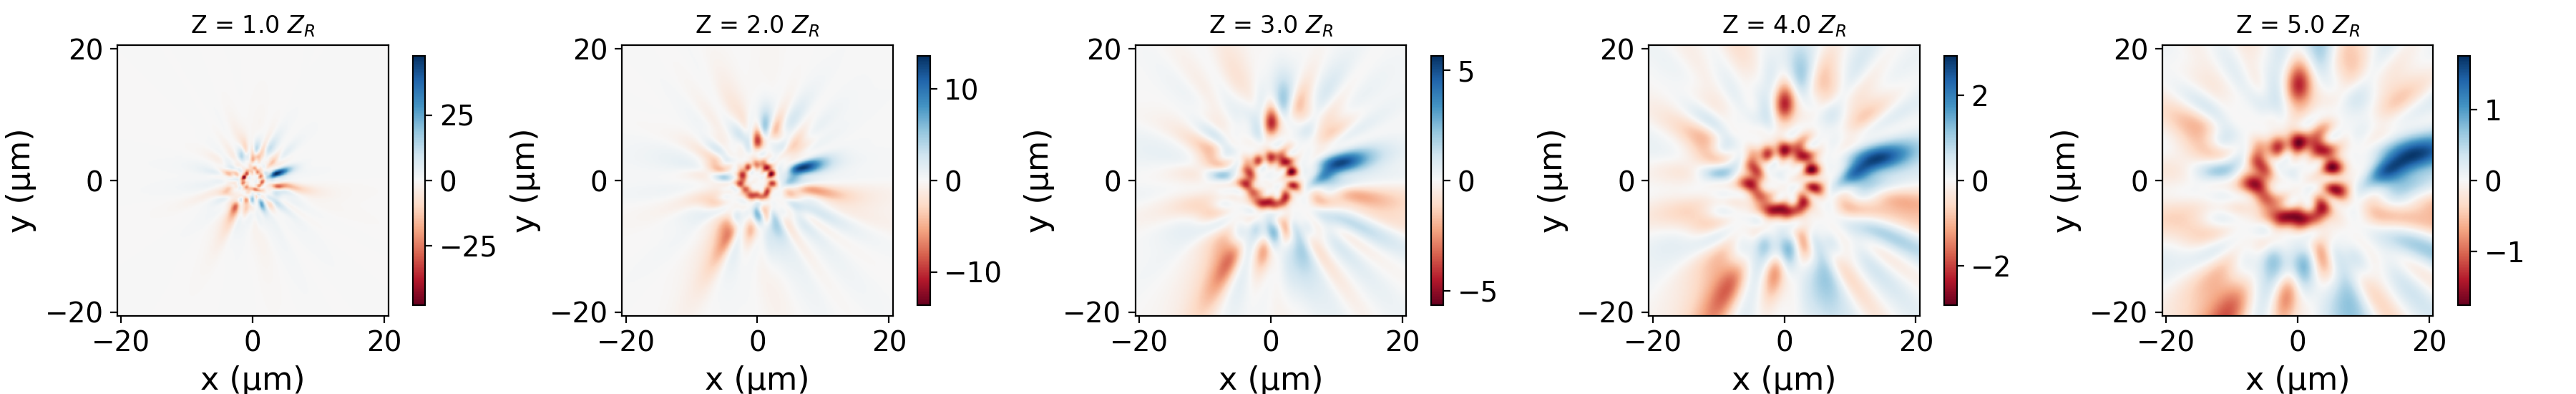
\includegraphics[width=1.0\textwidth]{img/chirality_prop_1to10zr_Fixed_XY_360_1.png}\\[2pt]
    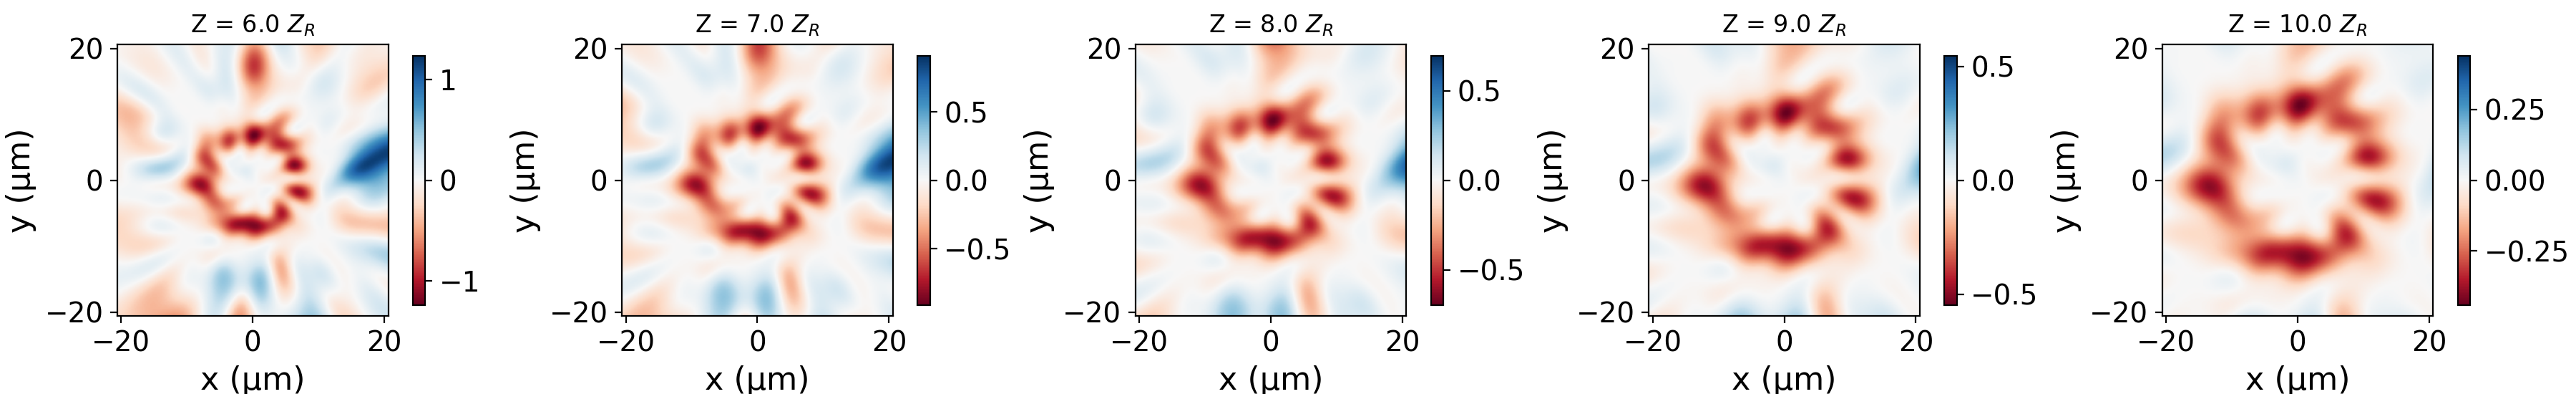
\includegraphics[width=1.0\textwidth]{img/chirality_prop_1to10zr_Fixed_XY_360_2.png}
\caption{Optical chirality propagation evolution for $\ell = 5$. Upper two rows: $z = 0.0z_{R}$ to $0.9z_{R}$; lower two rows: $z = 1.0z_{R}$ to $10.0z_{R}$. Color scale: blue ($C > 0$) indicates RCP dominance; red ($C < 0$) indicates LCP dominance. Near-field scattering creates a mixed LCP/RCP state; by $z \ge z_R$ the field is dominated by the LCP propagating mode.}
\label{fig:chirality_prop}
\end{figure}


\subsection{Near-Field Chirality}
\label{ssec:chirality_near}

Based on the propagation mechanism described above, Figure~\ref{fig:near_chirality_all} further shows the optical chirality density distributions (raw value $C$ and normalized value $C/|C|_\text{max}$) at the near-field monitor plane just above the design layer for $\ell = 0$ to $5$.

In the near-field region, the optical chirality shows a mixed LCP/RCP distribution, with a large fraction of the area exhibiting blue positive values ($C > 0$, i.e., RCP). This arises from the intense local scattering and evanescent wave coupling that the nanostructure induces in the near field, which generates significant local RCP components superimposed on the LCP-dominated source field.

\begin{figure}[htb]
\centering
	\begin{tabular}{cc} 
	    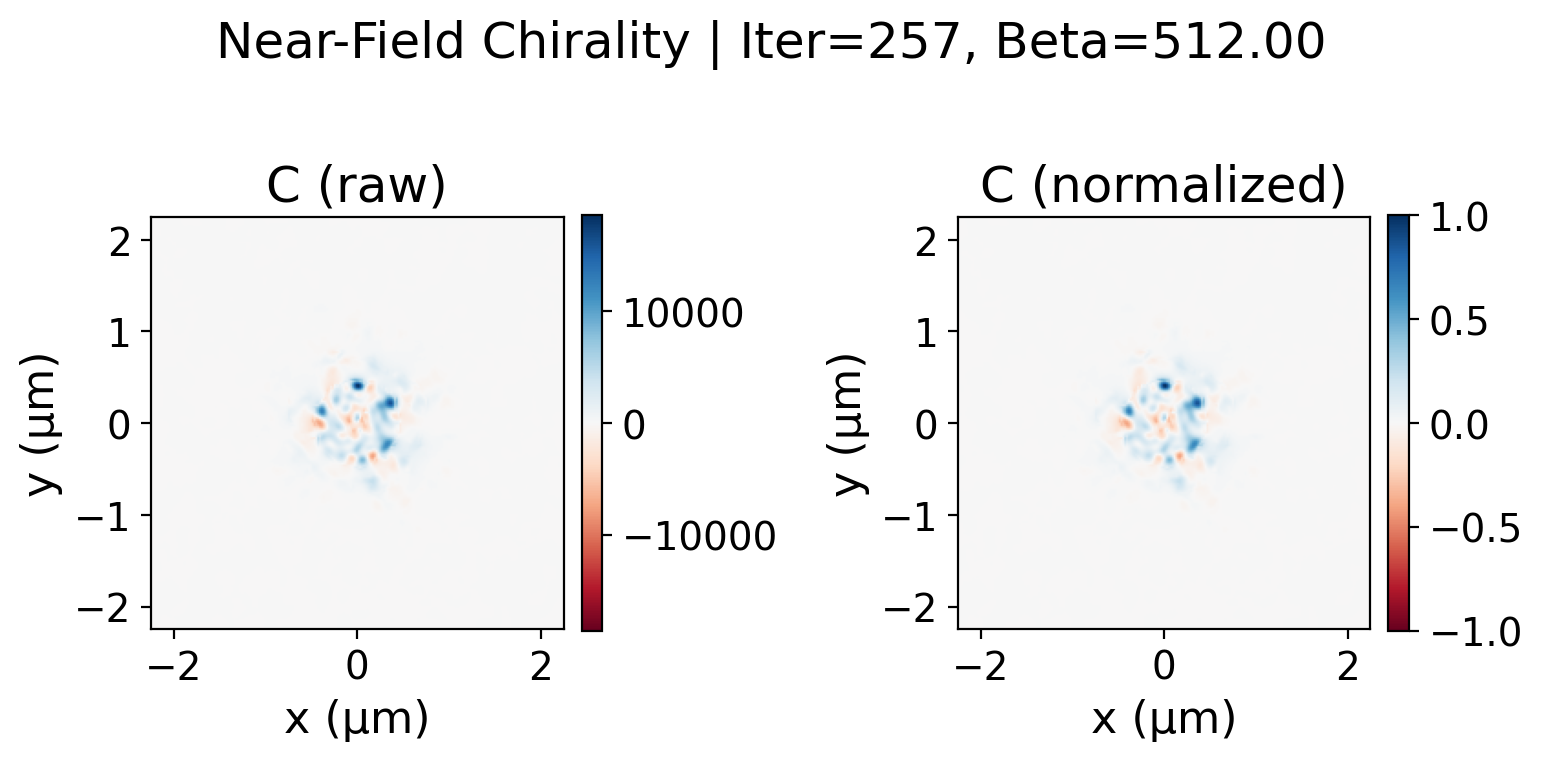
\includegraphics[width=0.47\textwidth]{img/017_near_chirality_257_beta_512.00.png}&
	    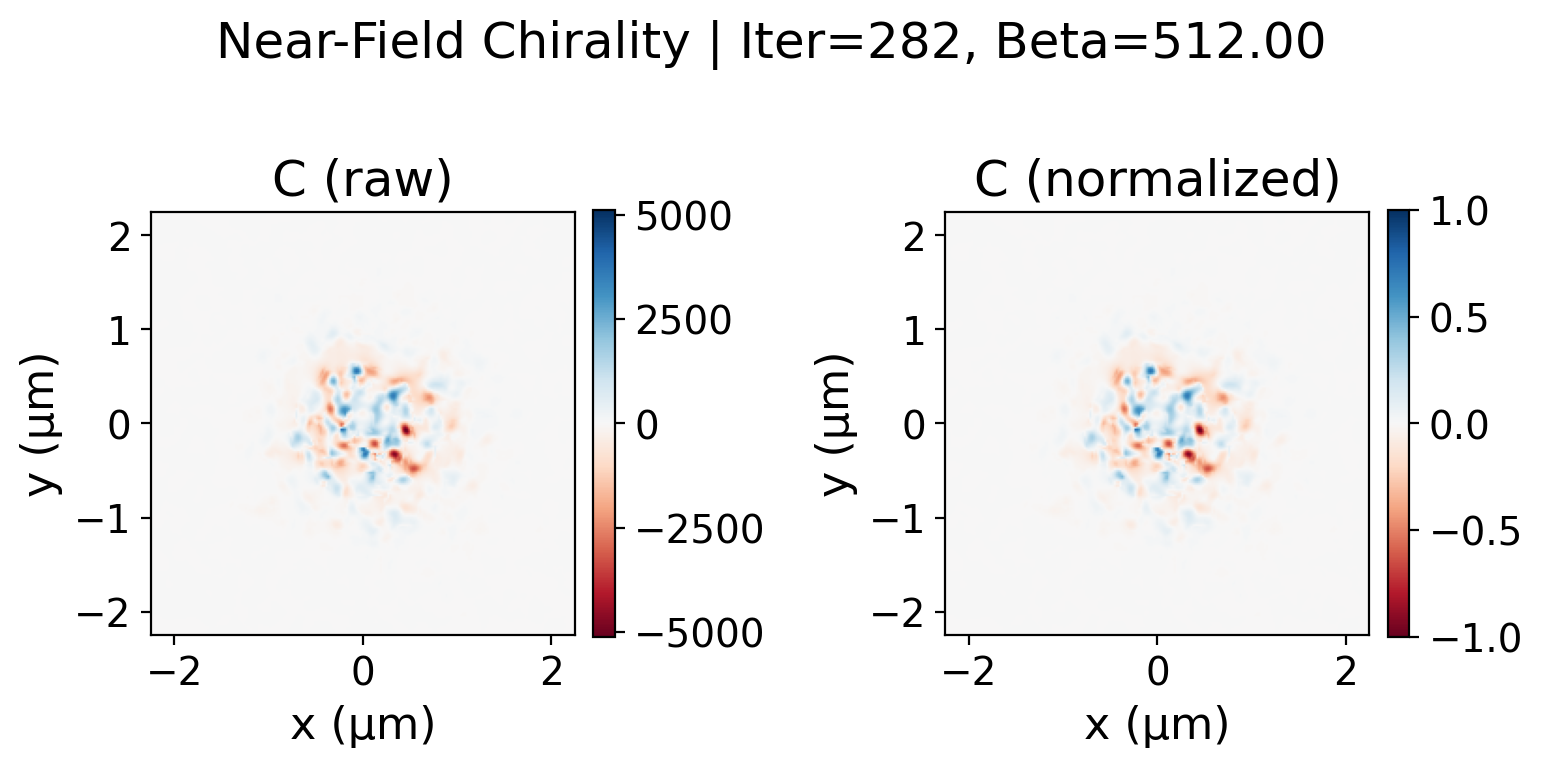
\includegraphics[width=0.47\textwidth]{img/018_near_chirality_282_beta_512.00.png}
		\\ (a) & (b)\\[6pt]
		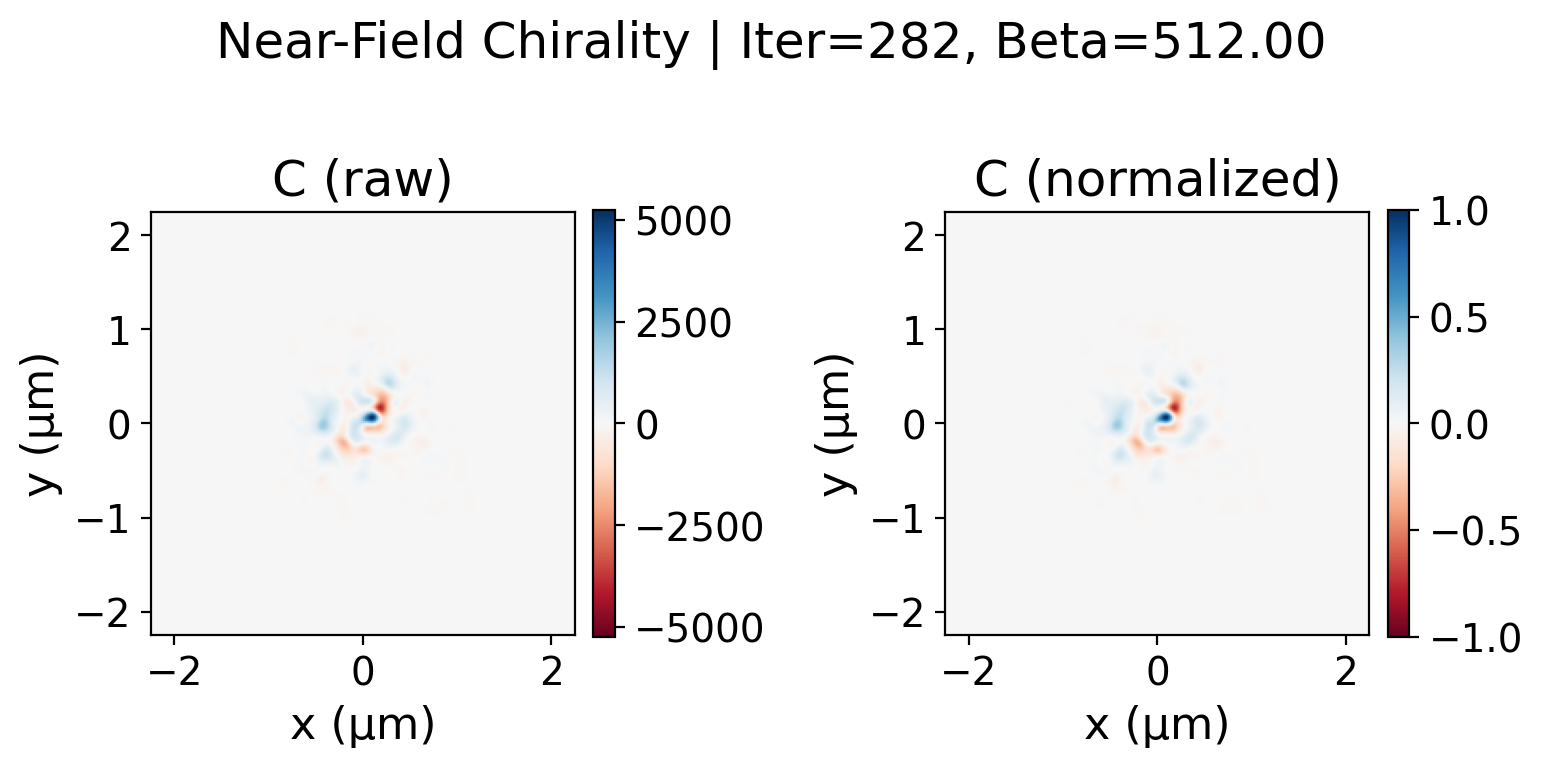
\includegraphics[width=0.47\textwidth]{img/013_near_chirality_282_beta_512.00.png}&
	    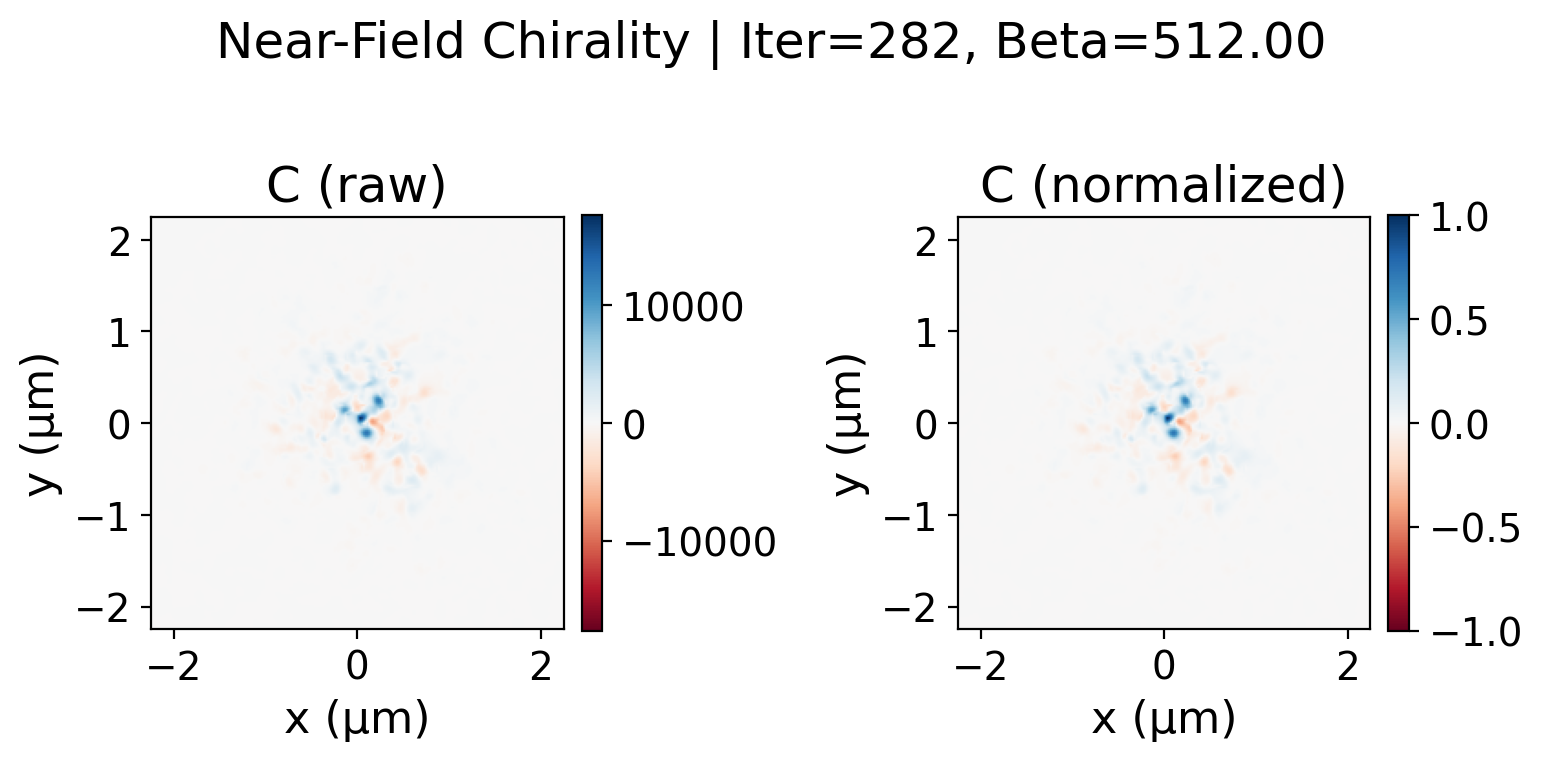
\includegraphics[width=0.47\textwidth]{img/020_near_chirality_282_beta_512.00.png}
	    \\(c) & (d)\\[6pt]
	    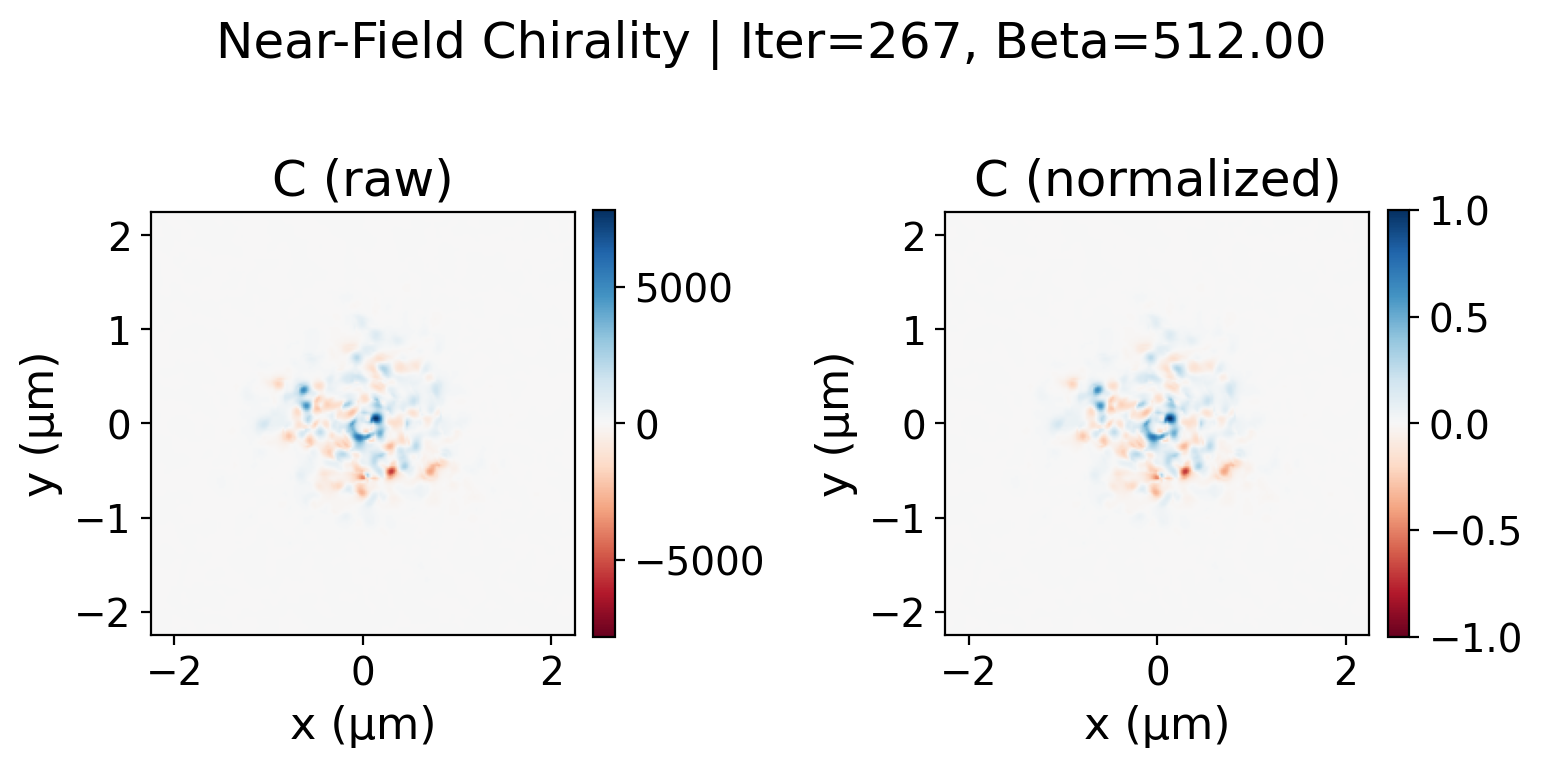
\includegraphics[width=0.47\textwidth]{img/021_near_chirality_267_beta_512.00.png}&
	    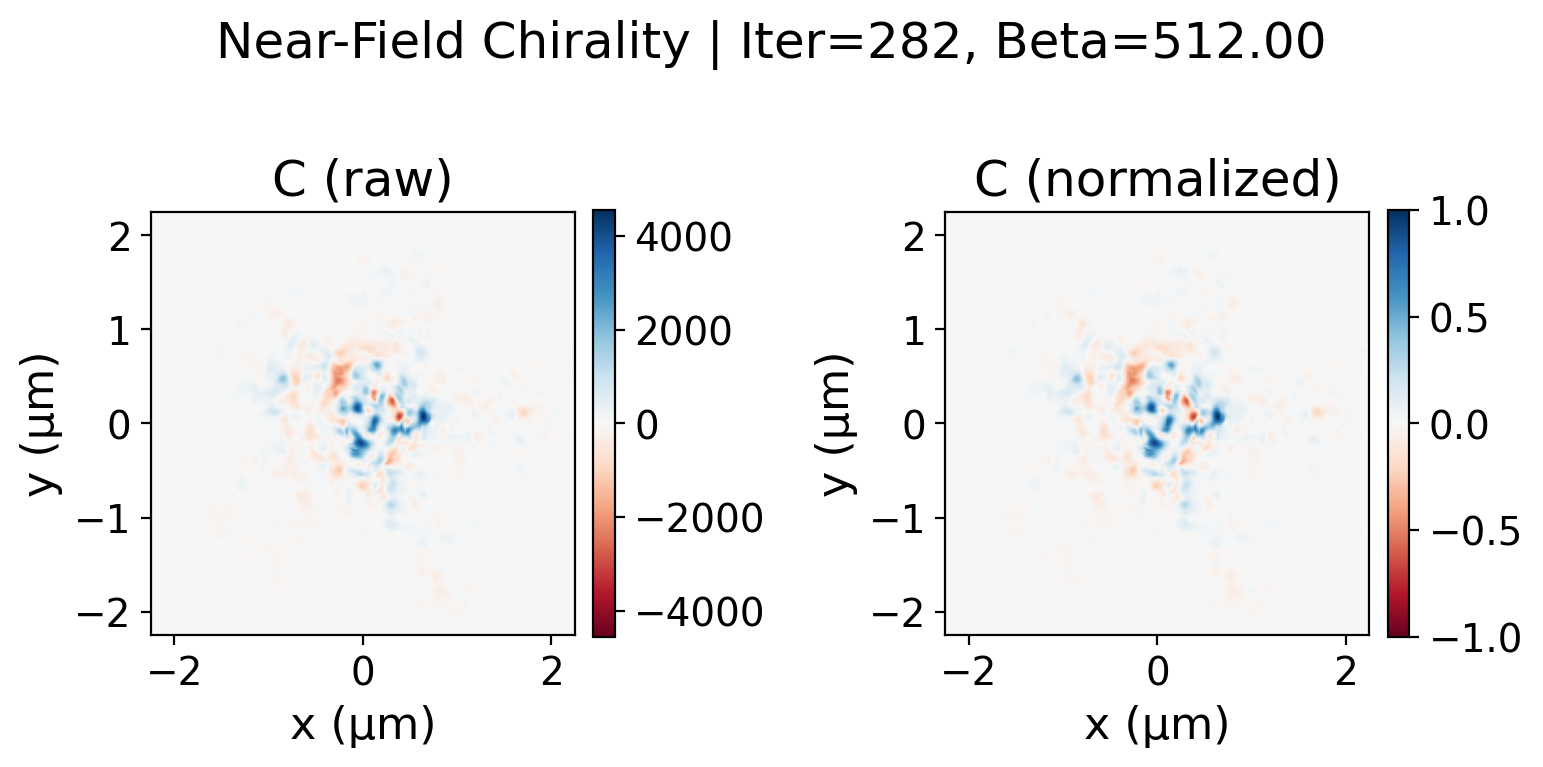
\includegraphics[width=0.47\textwidth]{img/022_near_chirality_282_beta_512.00.png}
	    \\(e) & (f)
	\end{tabular}
\caption{Near-field optical chirality density distributions: (a)$\sim$(f) $\ell \in \{0, 1, 2, 3, 4, 5\}$, respectively. Left column: raw chirality density $C$; right column: normalized chirality density $C/|C|_\text{max}$. The near field shows a mixed LCP/RCP distribution with LCP occupying the majority.}
\label{fig:near_chirality_all}
\end{figure}

\subsection{Far-Field Chirality}
\label{ssec:chirality_far}

Figure~\ref{fig:ff_chirality_all} shows the optical chirality density distributions at the far-field evaluation plane ($z = 10\,z_R$) for $\ell = 0$ to $5$.

Unlike the mixed state in the near field, the far-field chirality density within the main spot region is uniformly and purely negative (red, $C < 0$), meaning the beam has fully recovered to LCP handedness consistent with the K-valley LCP source polarization after propagating to the far field. It is worth noting that the geometric outline of the far-field optical chirality density perfectly overlaps with the far-field intensity distribution. Physically, the chirality distribution closely follows the intensity, confirming that the far-field polarization is highly uniform across the beam cross-section---the beam maintains pure LCP circular polarization everywhere, and the edge decay of the chirality density is only due to intensity falloff, not degradation in polarization quality. This consistent geometric character also indicates that the nanostructure, while performing OAM phase reshaping, effectively decouples spin and orbital angular momentum without introducing unintended spin-orbit coupling effects, ensuring the far-field radiation has very high polarization purity and mode quality.

\begin{figure}[htb]
\centering
	\begin{tabular}{cc} 
	    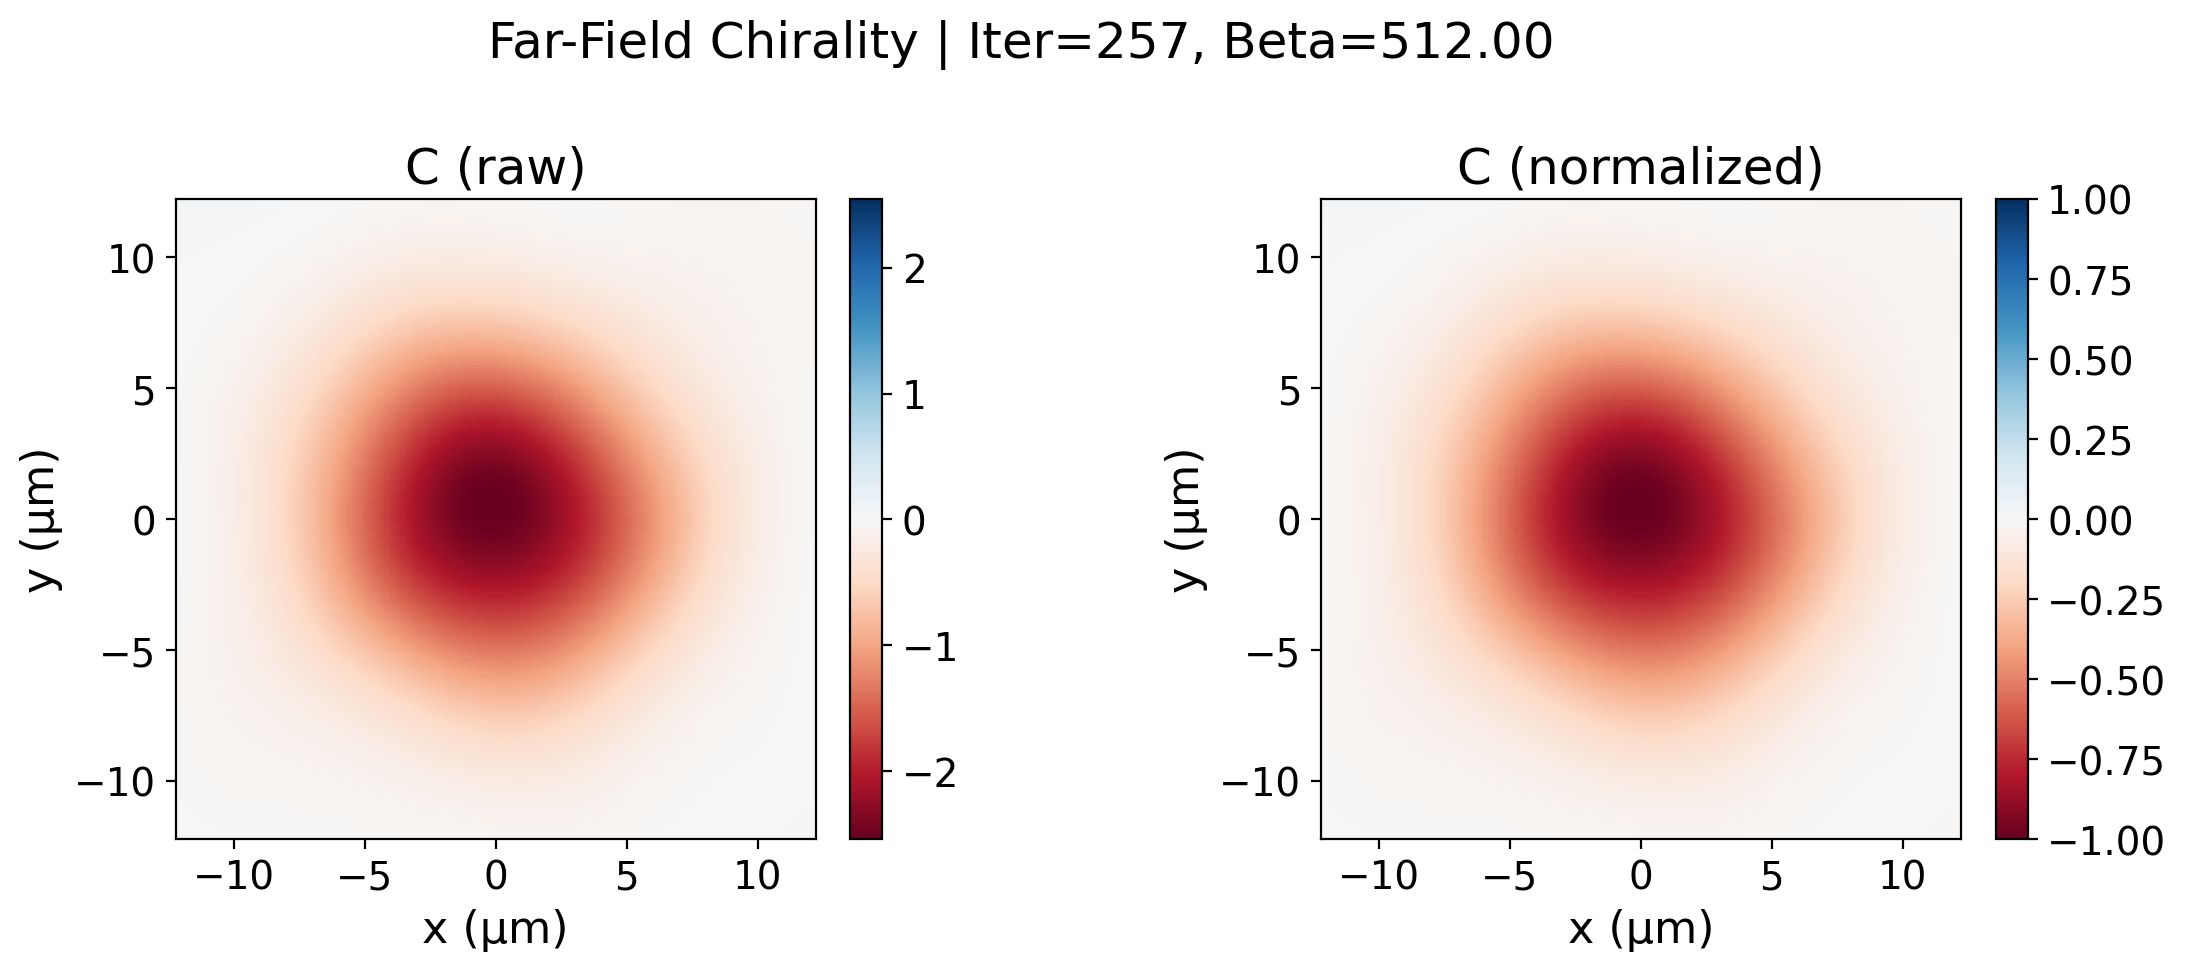
\includegraphics[width=0.47\textwidth]{img/017_ff_chirality_257_beta_512.00.png}&
	    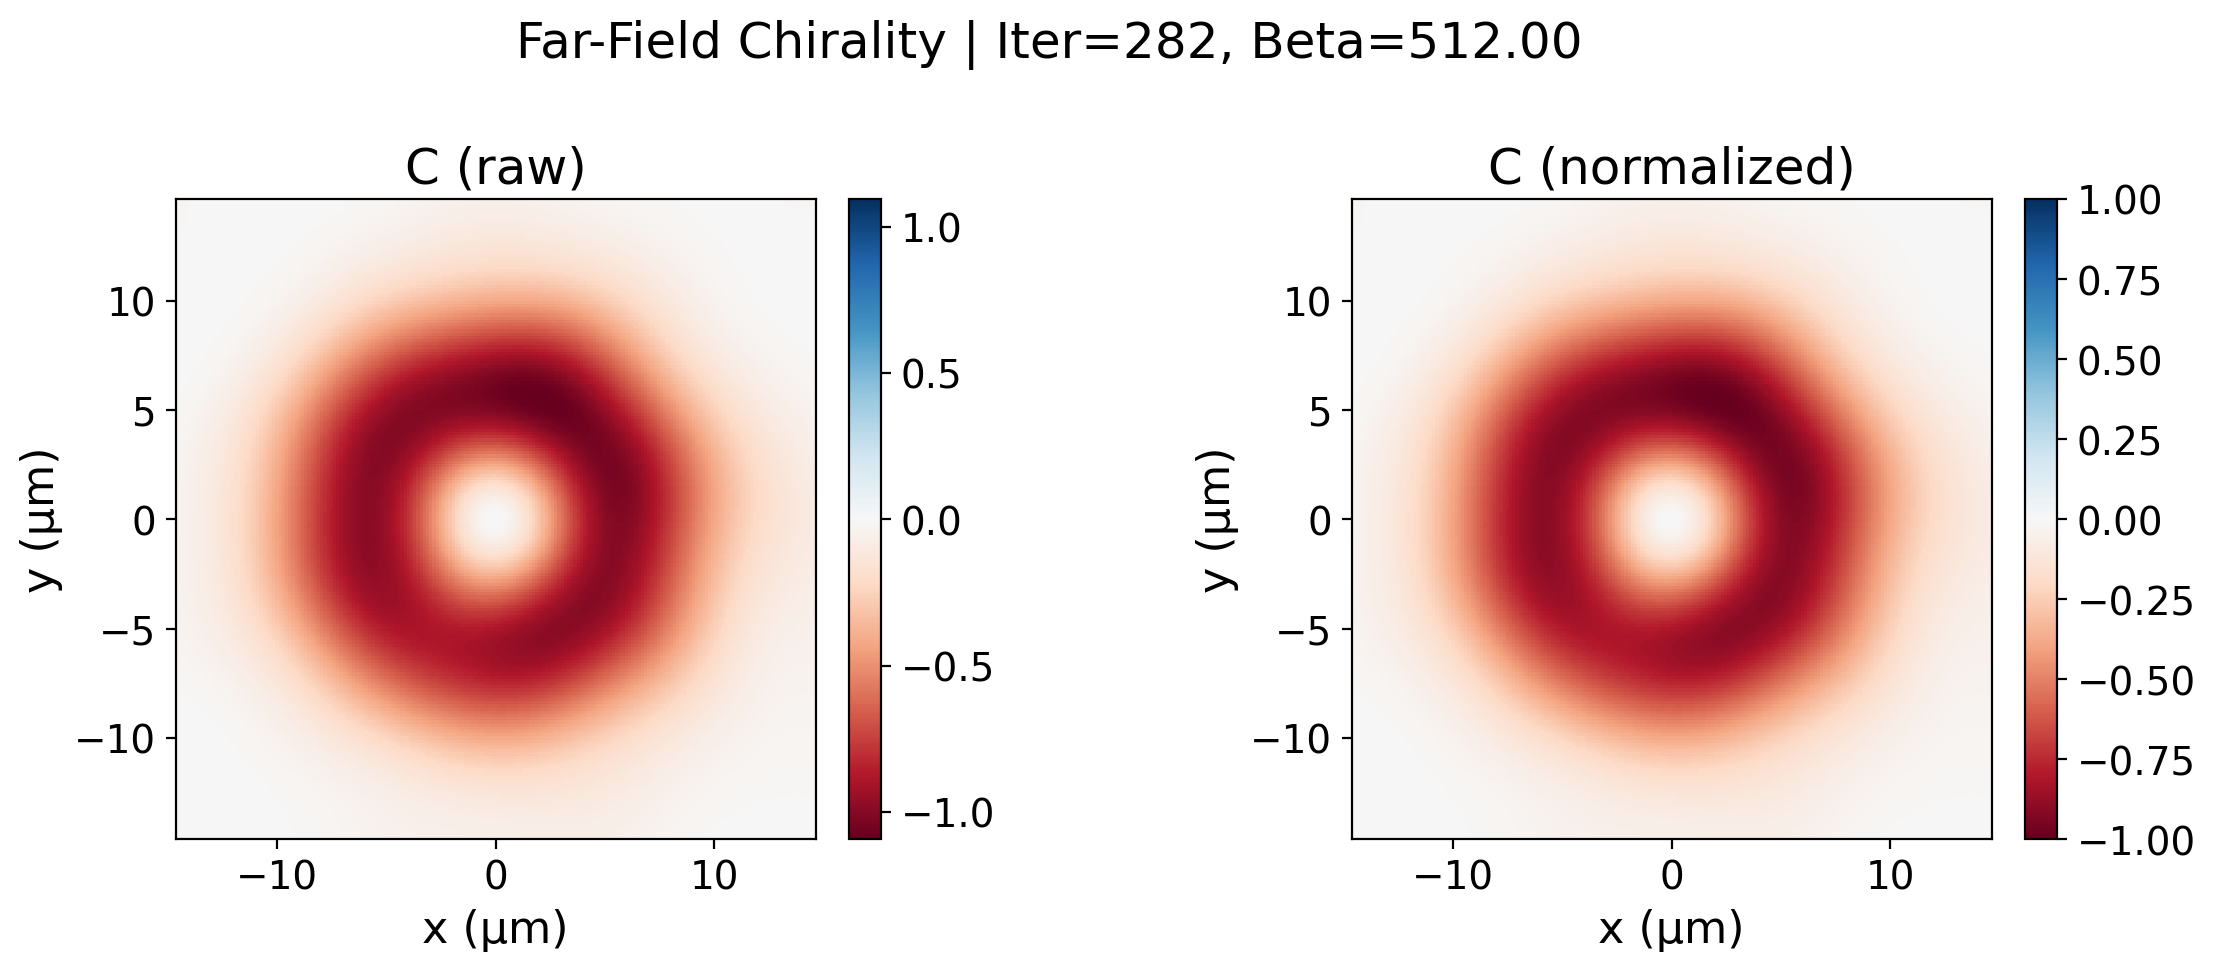
\includegraphics[width=0.47\textwidth]{img/018_ff_chirality_282_beta_512.00.png}
		\\ (a) & (b)\\[6pt]
		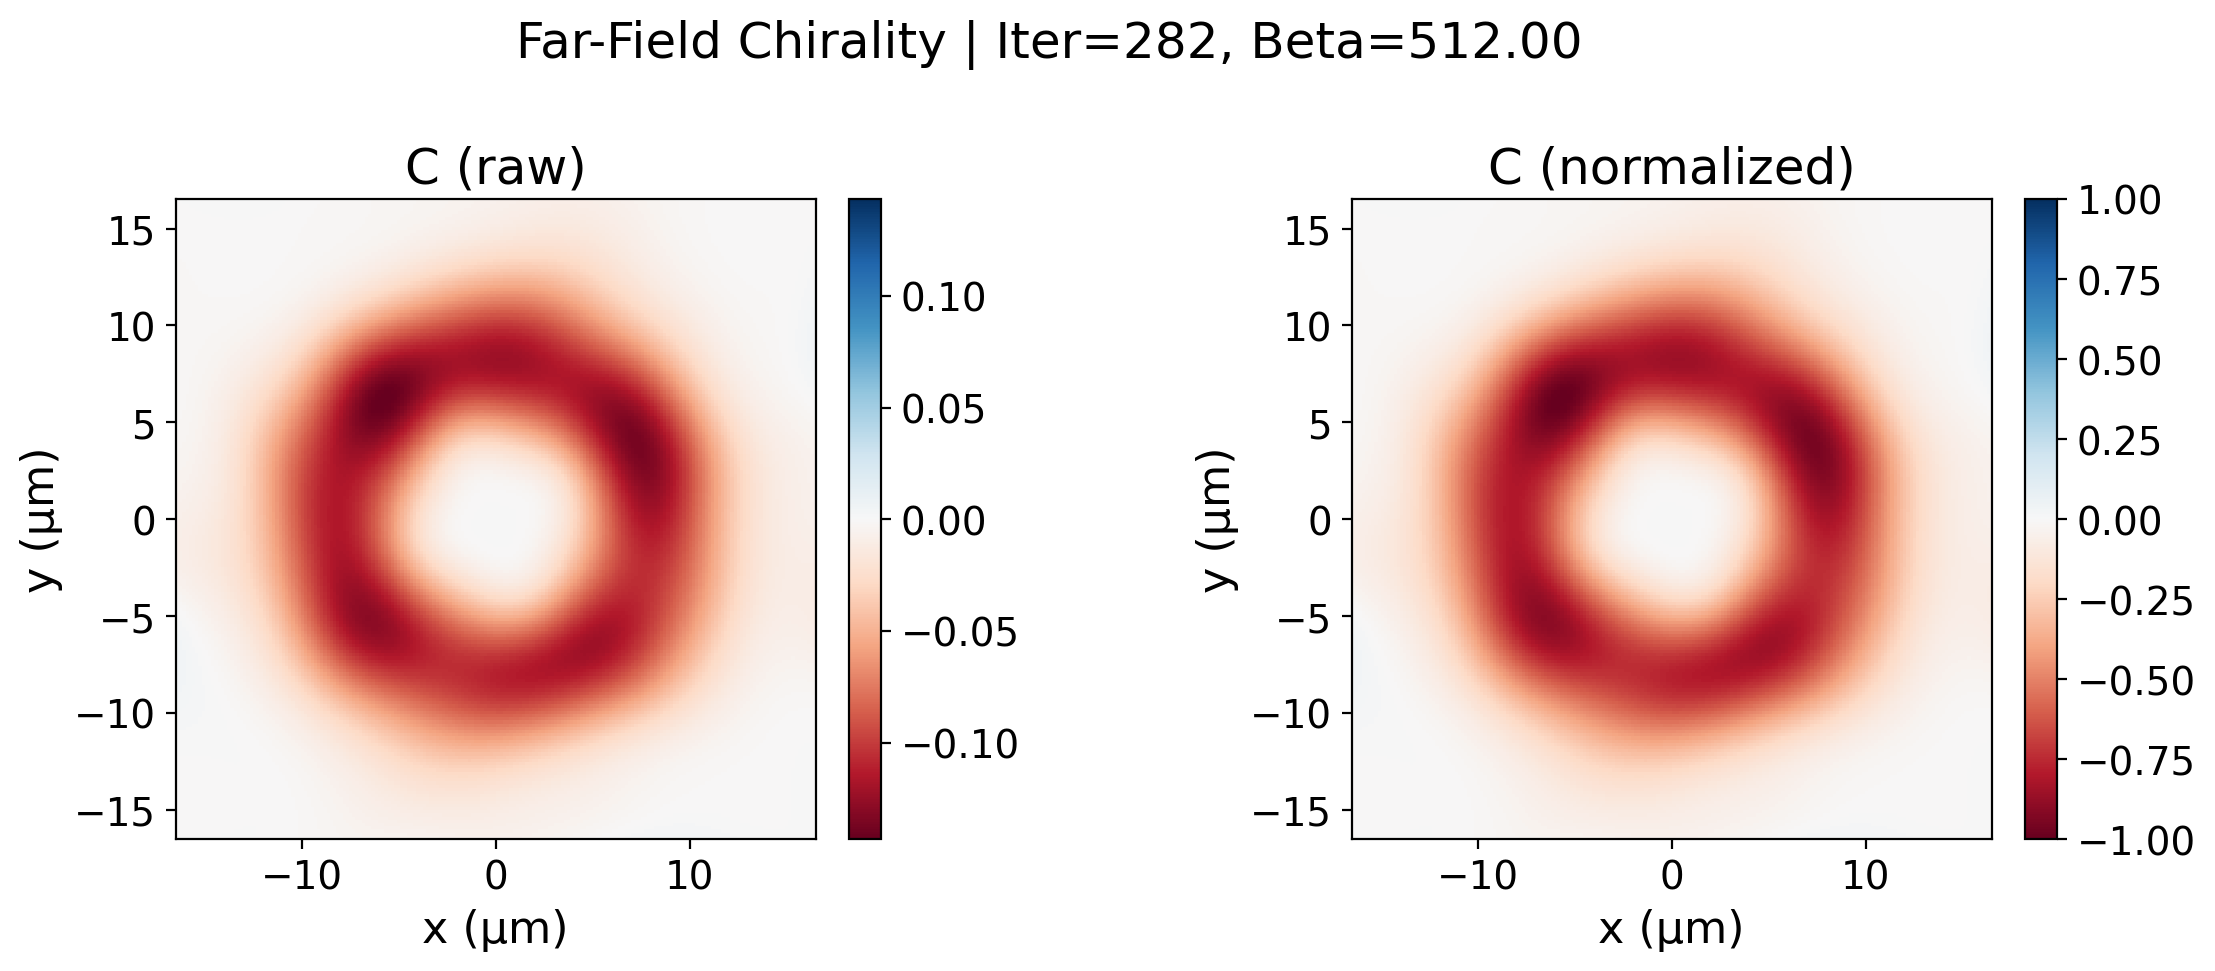
\includegraphics[width=0.47\textwidth]{img/013_ff_chirality_282_beta_512.00.png}&
	    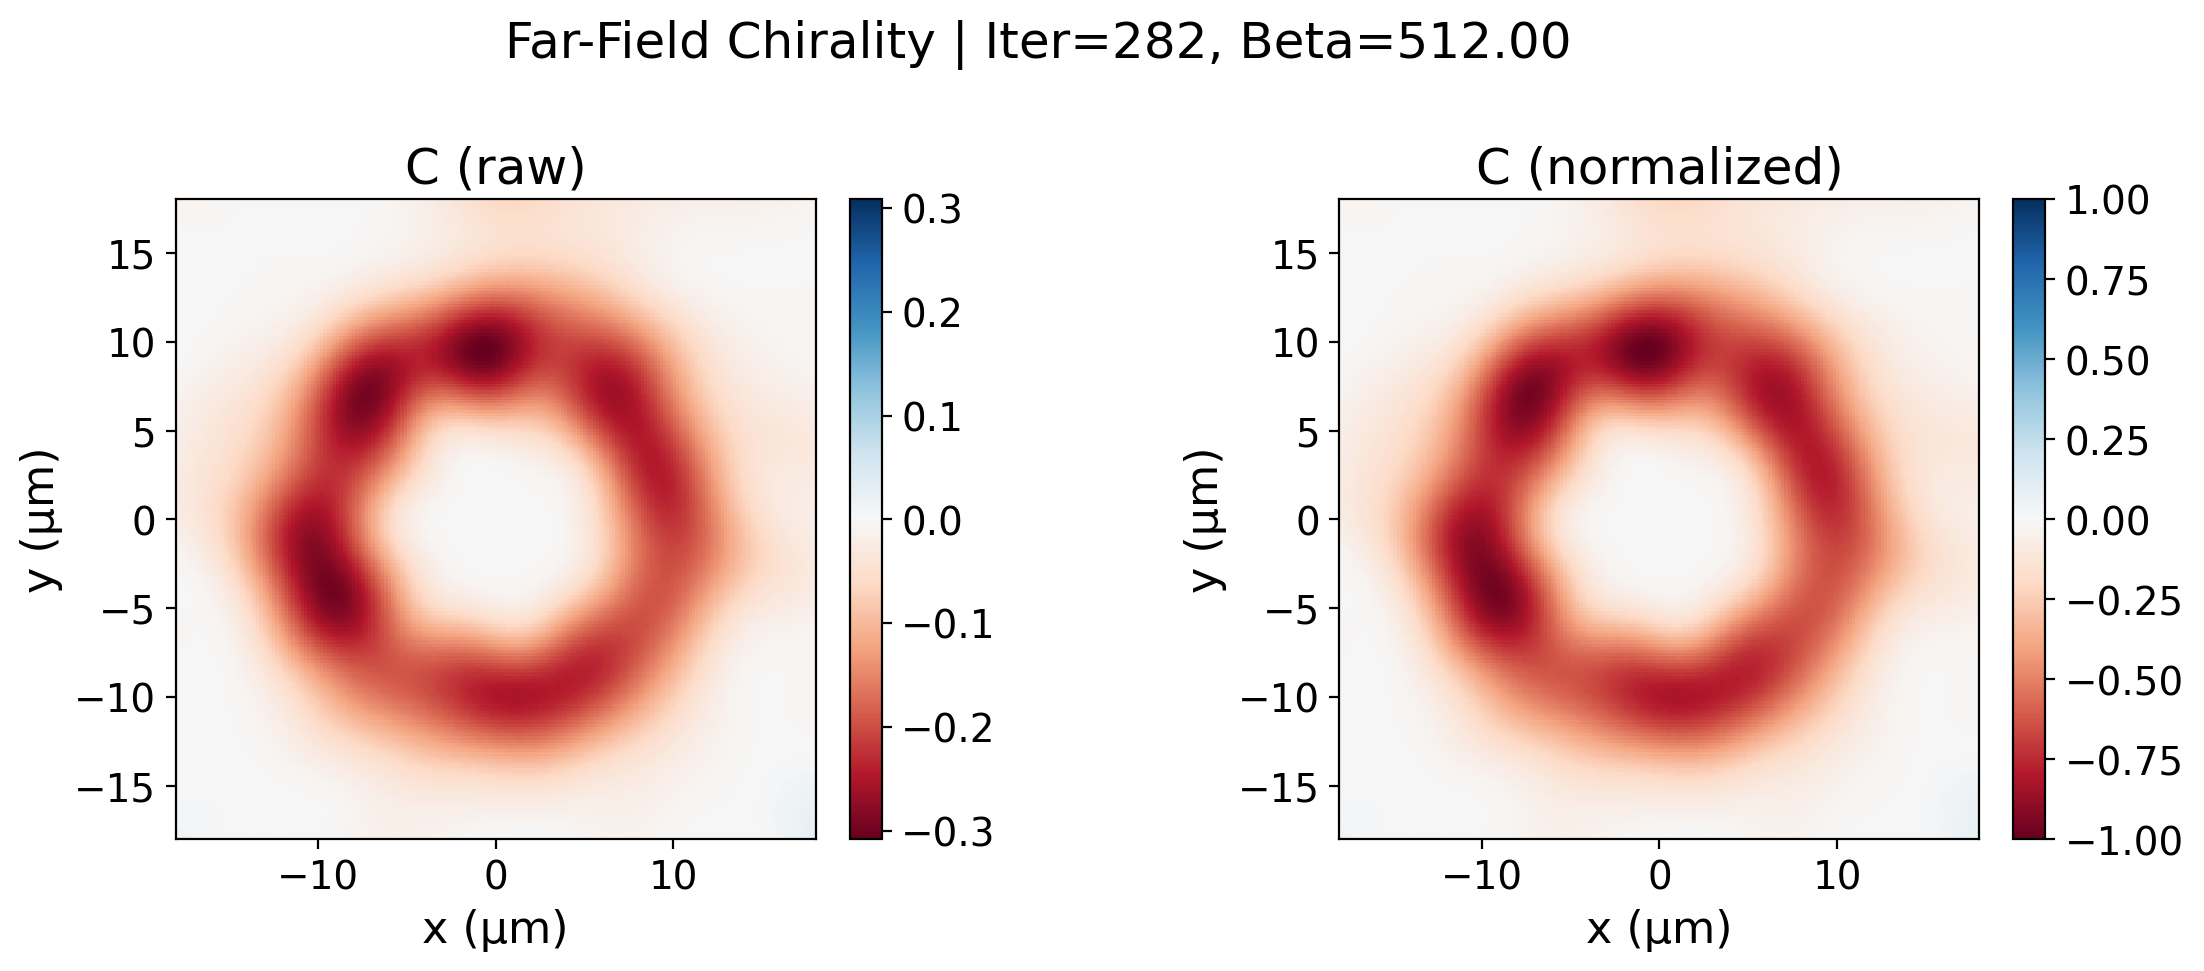
\includegraphics[width=0.47\textwidth]{img/020_ff_chirality_282_beta_512.00.png}
	    \\(c) & (d)\\[6pt]
	    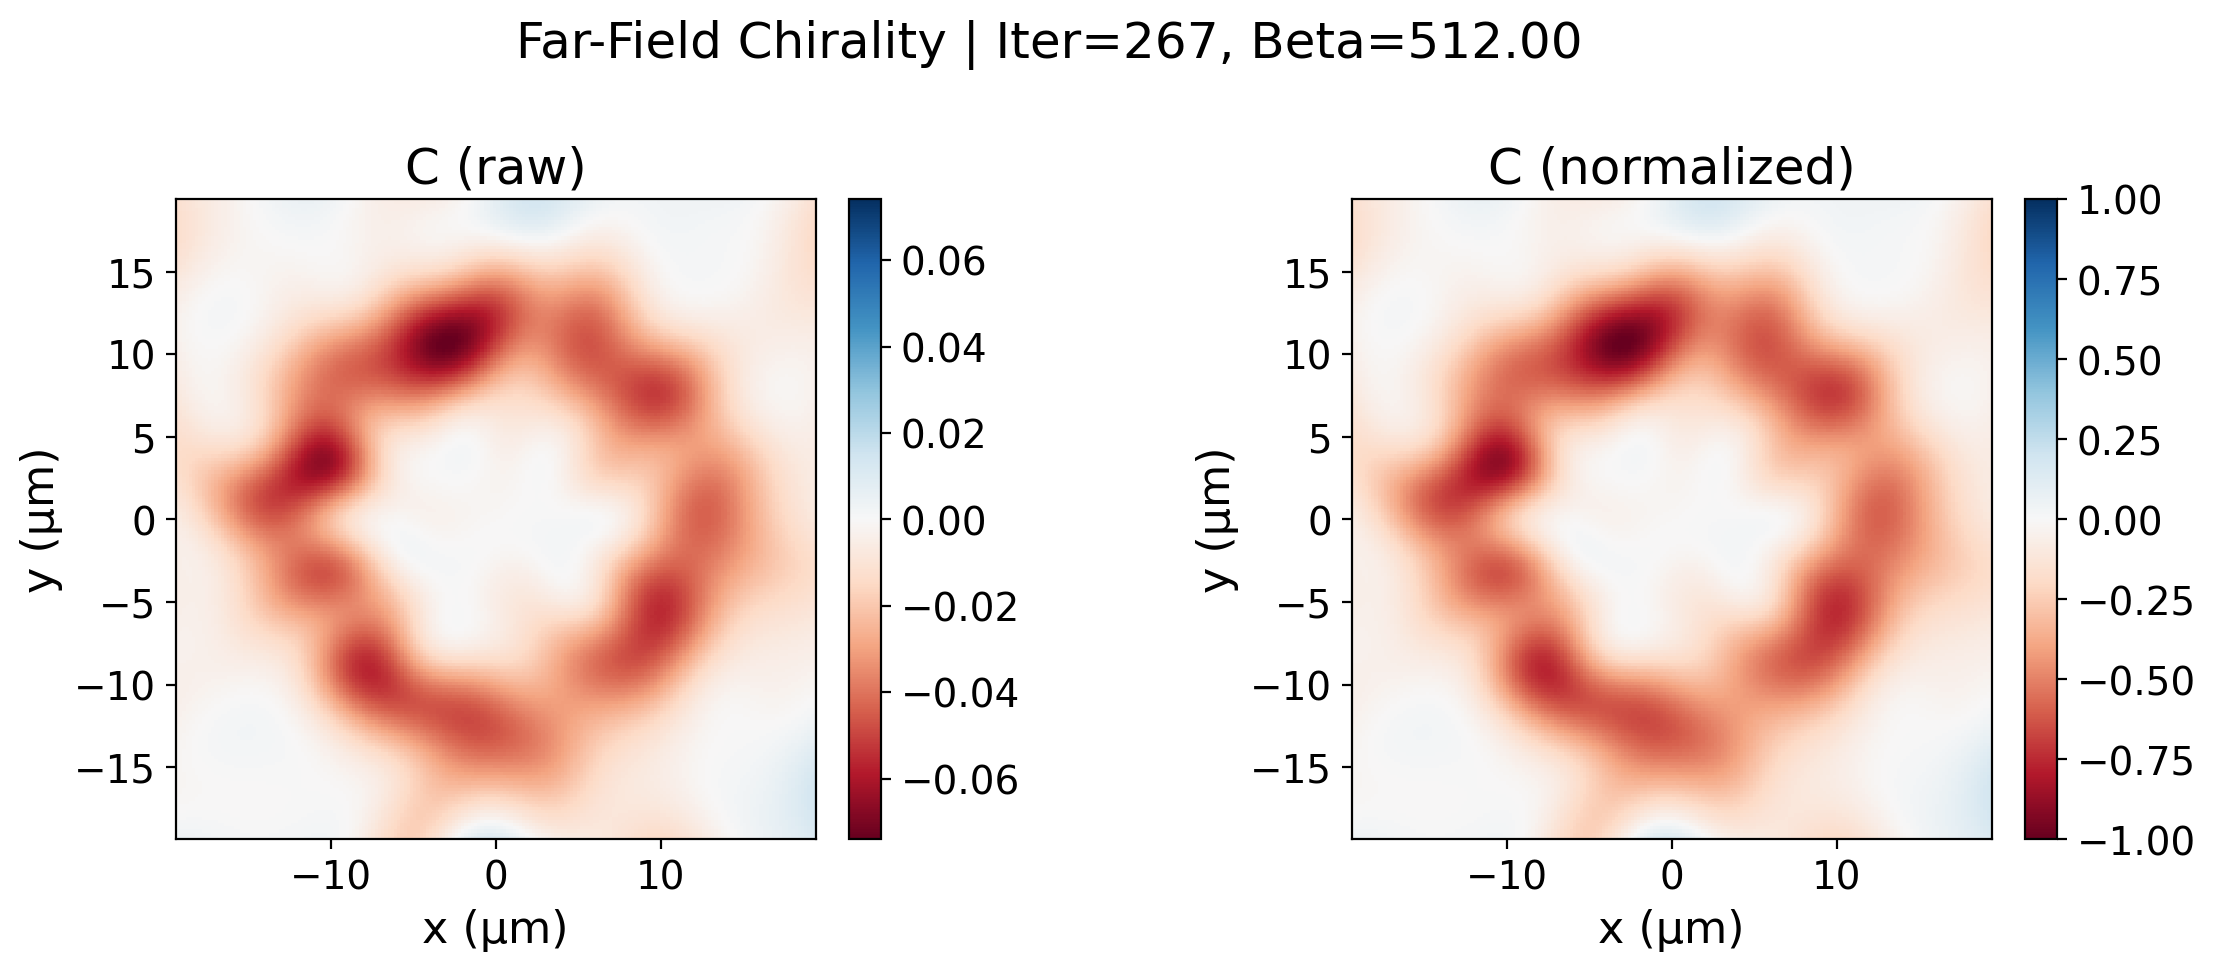
\includegraphics[width=0.47\textwidth]{img/021_ff_chirality_267_beta_512.00.png}&
	    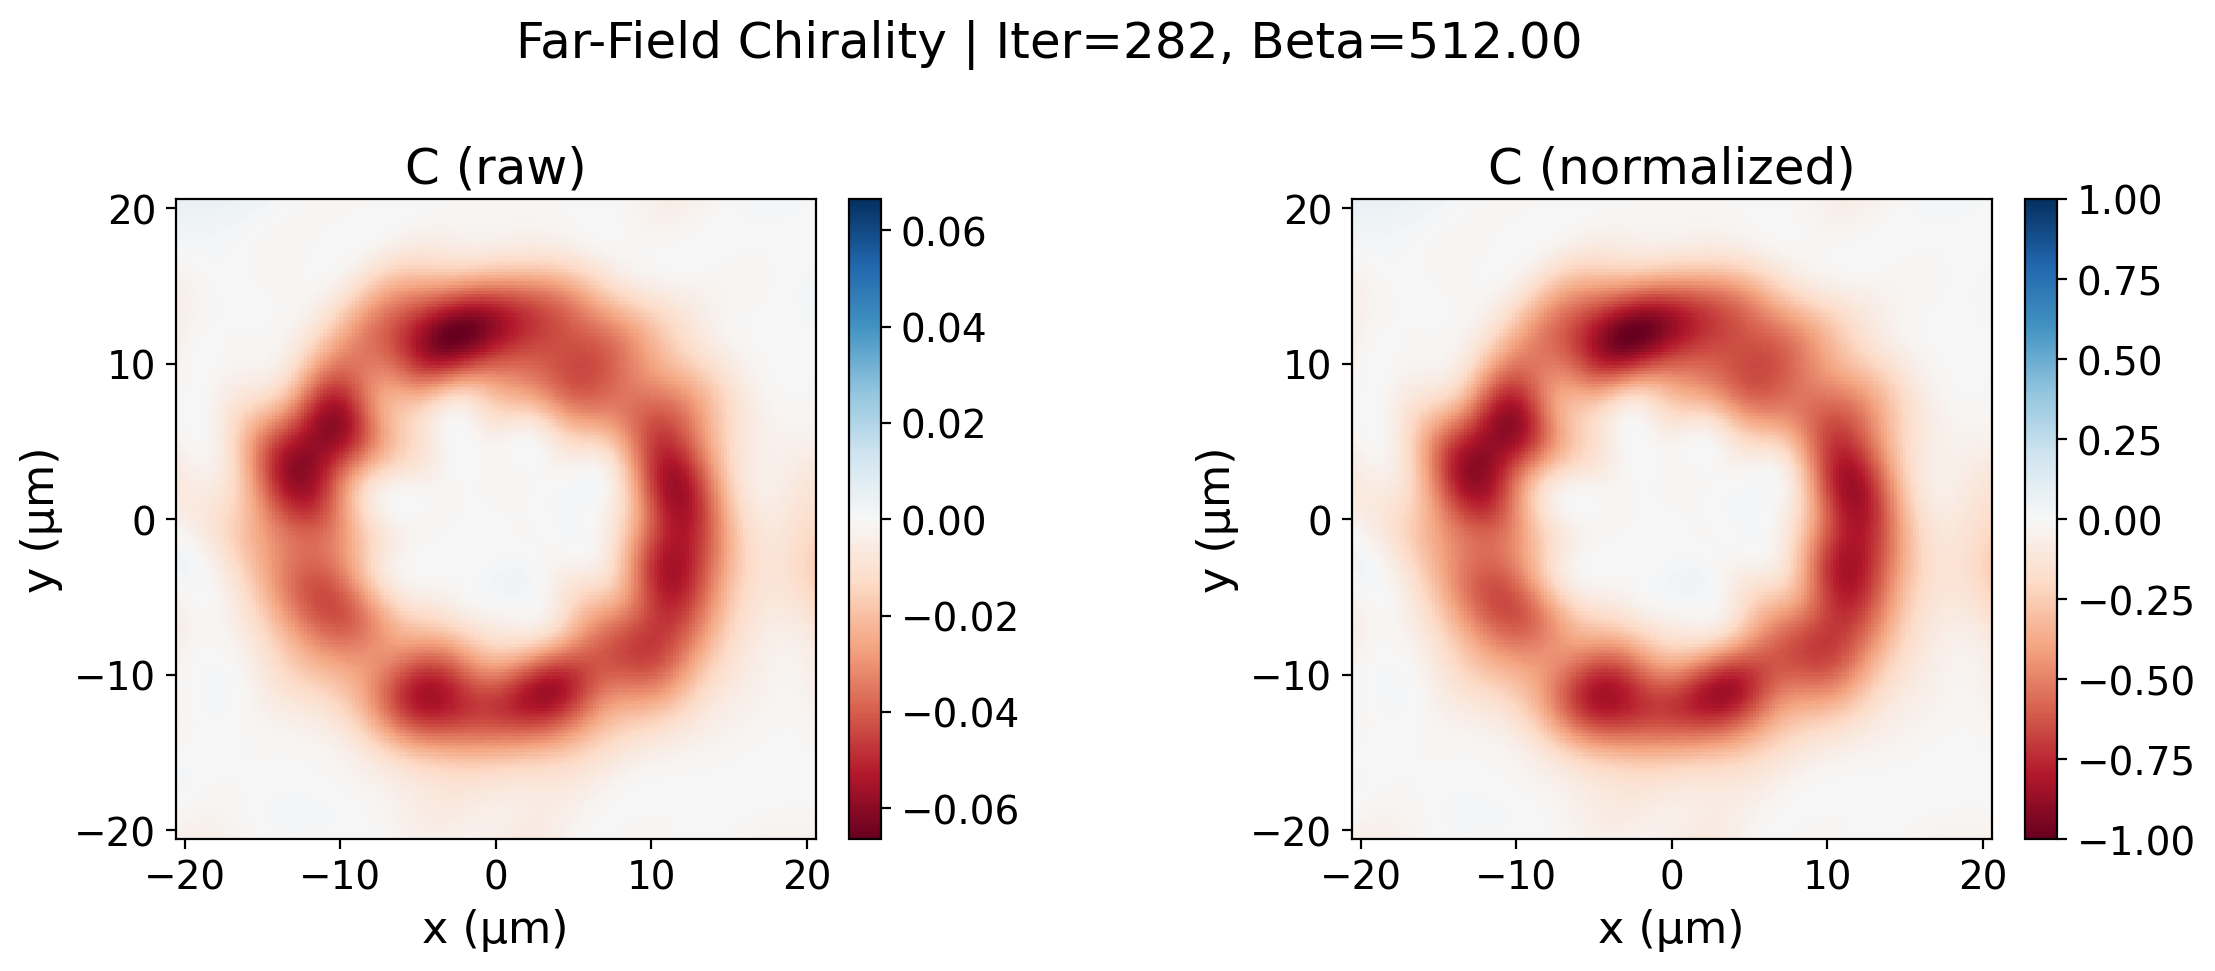
\includegraphics[width=0.47\textwidth]{img/022_ff_chirality_282_beta_512.00.png}
	    \\(e) & (f)
	\end{tabular}
\caption{Far-field optical chirality density distributions ($z = 10\,z_R$): (a)$\sim$(f) $\ell \in \{0, 1, 2, 3, 4, 5\}$, respectively. Left column: raw chirality density $C$; right column: normalized chirality density $C/|C|_\text{max}$. Within the far-field spot, purely uniform RCP (red negative values) chirality is observed.}
\label{fig:ff_chirality_all}
\end{figure}


%===================================================================


\section{Phase Winding Verification}

\label{sec:winding}

Phase winding analysis is the direct method for verifying the topological charge of the far-field vortex beam: the LCP electric field phase is sampled along a circular path at the far-field intensity peak radius $r_\text{peak}$; after unwrapping, the total azimuthal phase change is calculated, which should ideally equal $\ell \times 2\pi$.

Figure~\ref{fig:winding_all} shows the phase winding verification results for the six designs. After sampling along a circular path at the corresponding $r_\text{fraction}$ (ratio of peak radius to evaluation region radius) for each design, the agreement between the unwrapped phase (orange solid line) and the ideal $\ell \times 2\pi$ linear slope (black dashed line) is as follows:
\begin{table}[htb]
\centering
\caption{Phase winding verification results across target topological charges.}
\label{tab:phase_winding}
\begin{tabular}{cccc}
\toprule
$\ell$ & $r_\text{frac}$ & Total Unwrapped Phase & Phase Error \\
\midrule
0 & 0.2000 & $\approx 0 \times 2\pi$ & --- \\
1 & 0.3885 & $1.00 \times 2\pi$ & $< 0.1\%$ \\
2 & 0.4878 & $1.99 \times 2\pi$ & $0.5\%$ \\
3 & 0.5468 & $\approx 3.00 \times 2\pi$ & $< 1\%$ \\
4 & 0.5868 & $\approx 4.00 \times 2\pi$ & $< 1\%$ \\
5 & 0.6176 & $\approx 5.00 \times 2\pi$ & $< 1\%$ \\
\bottomrule
\end{tabular}
\end{table}

The unwrapped phase for all designs closely matches the theoretical prediction, precisely verifying that each design does indeed generate a vortex beam with the target topological charge in the far field. Although the intensity ring for $\ell = 4, 5$ shows slight azimuthal non-uniformity (see Section~\ref{sec:farfield}), the phase winding still accurately reflects the corresponding topological charge. This indicates that the loss of high purity mainly comes from deviations in the intensity profile rather than misalignment of the phase singularity or a change in the topological charge.
\begin{figure}[htb]
\centering
	\begin{tabular}{cc} 
	    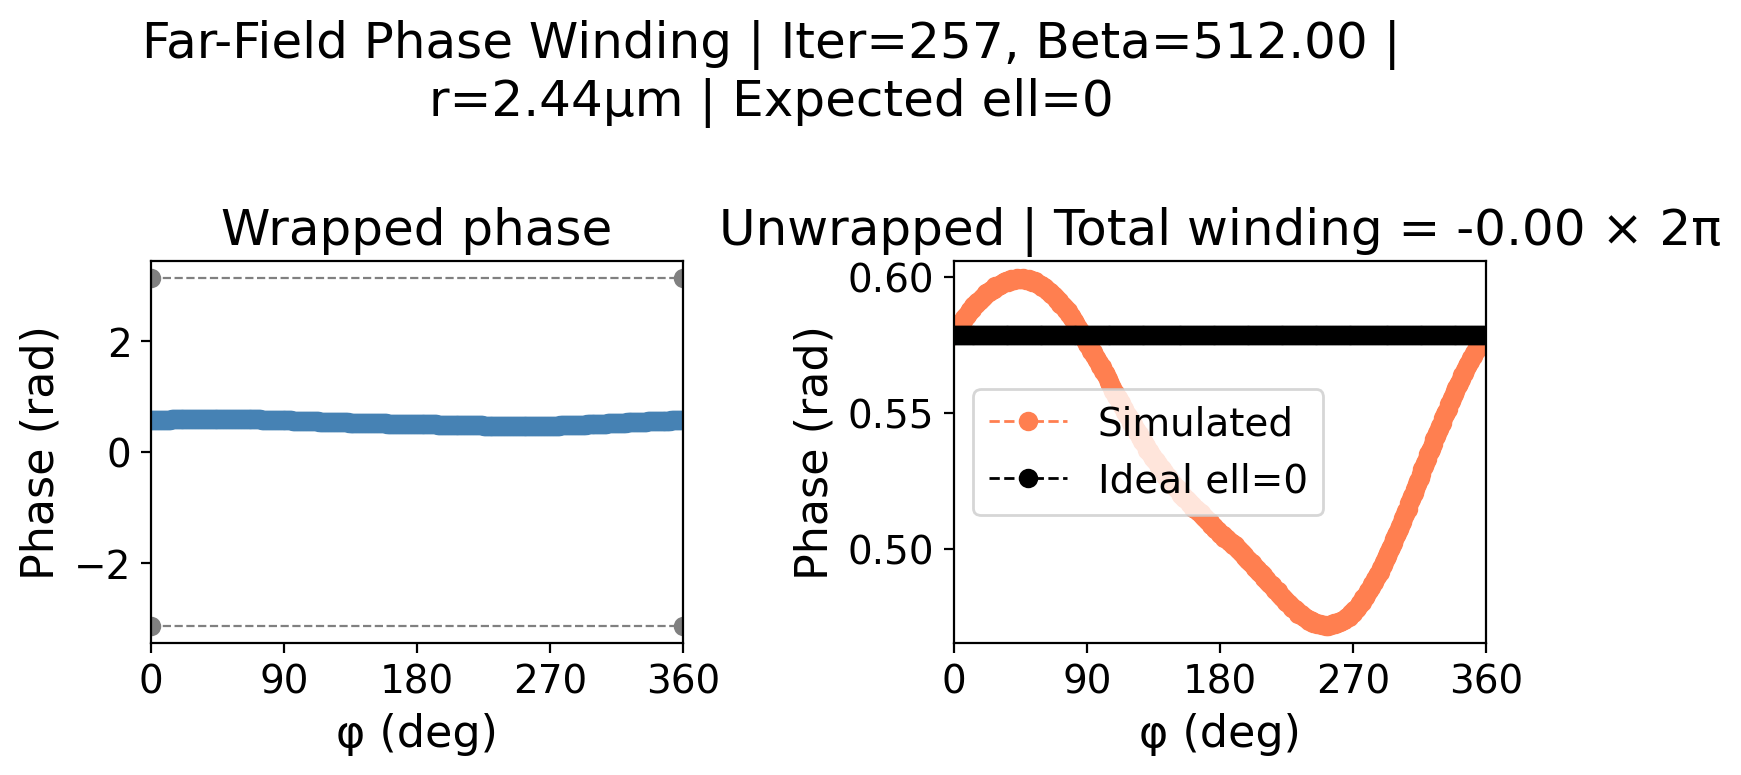
\includegraphics[width=0.47\textwidth]{img/017_ff_winding_iter_257_beta_512.00_rfraction_0.2000.png}&
	    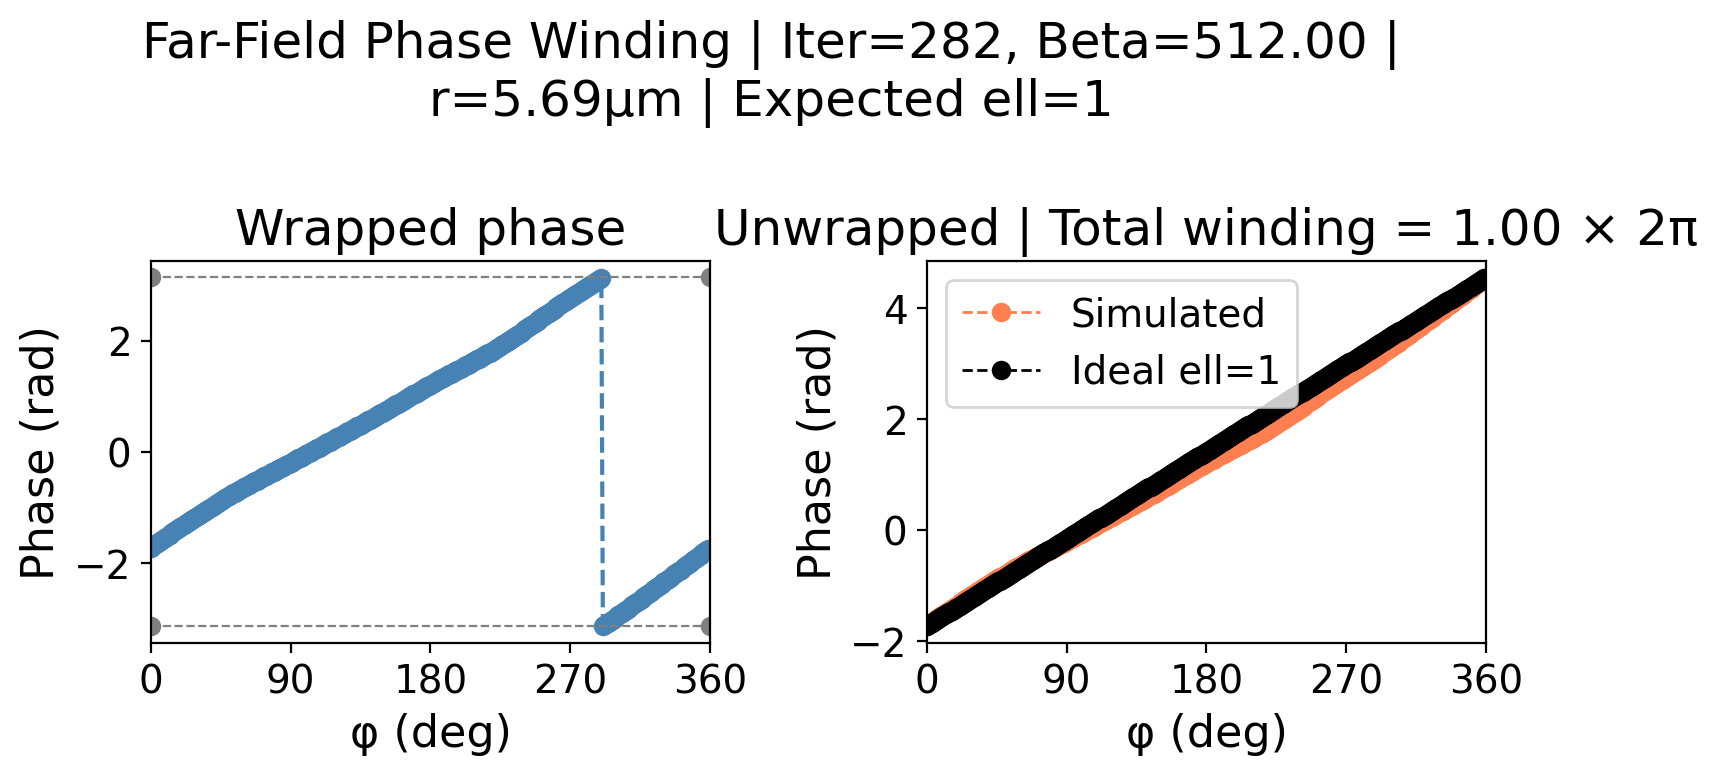
\includegraphics[width=0.47\textwidth]{img/018_ff_winding_iter_282_beta_512.00_rfraction_0.3885.png}
		\\ (a) & (b)\\[6pt]
		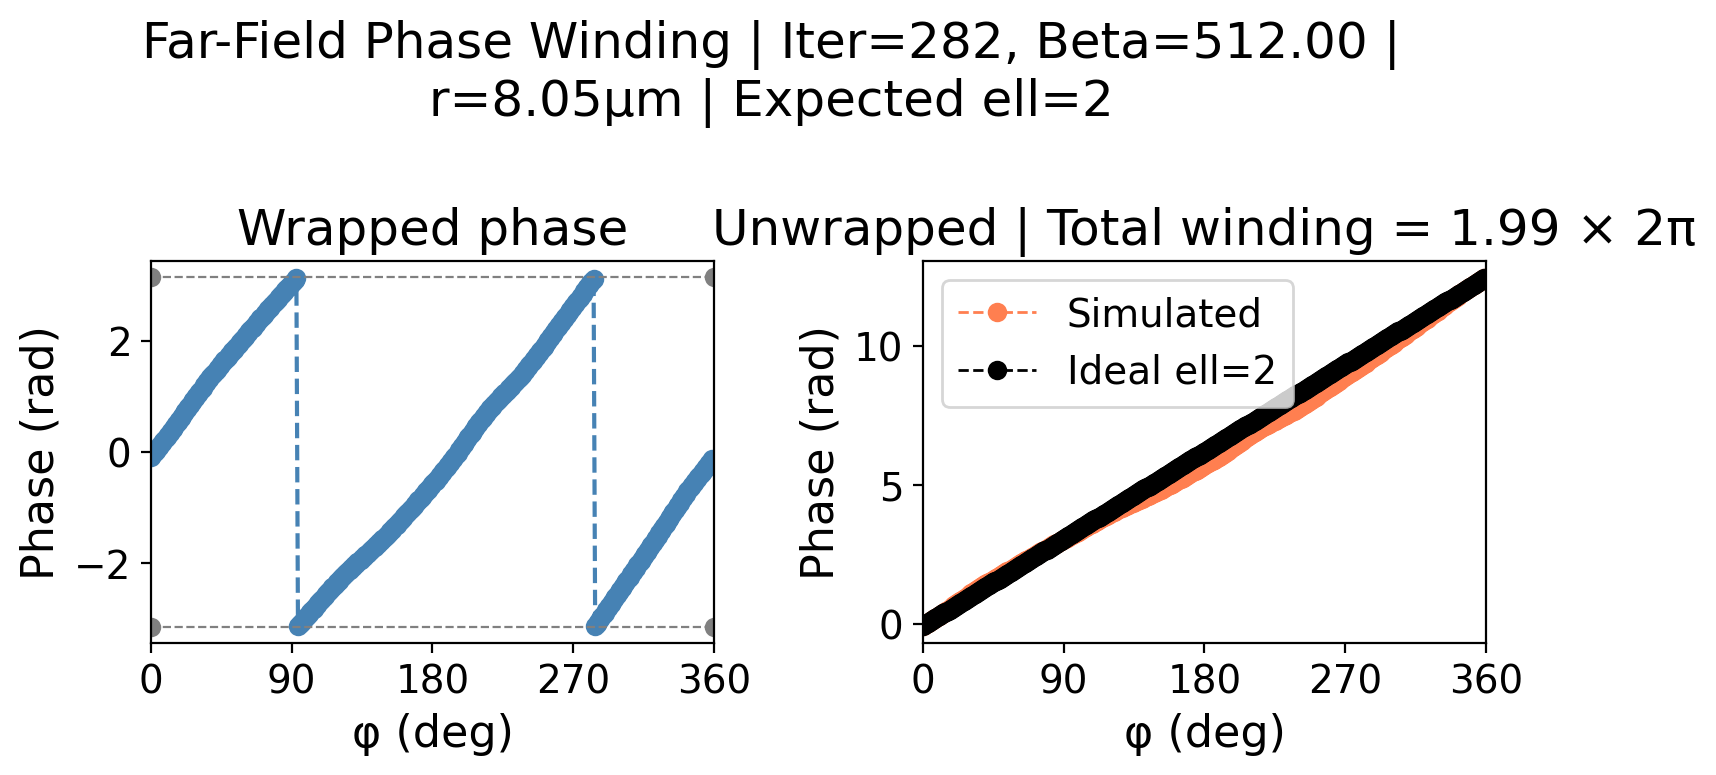
\includegraphics[width=0.47\textwidth]{img/013_ff_winding_iter_282_beta_512.00_rfraction_0.4878.png}&
	    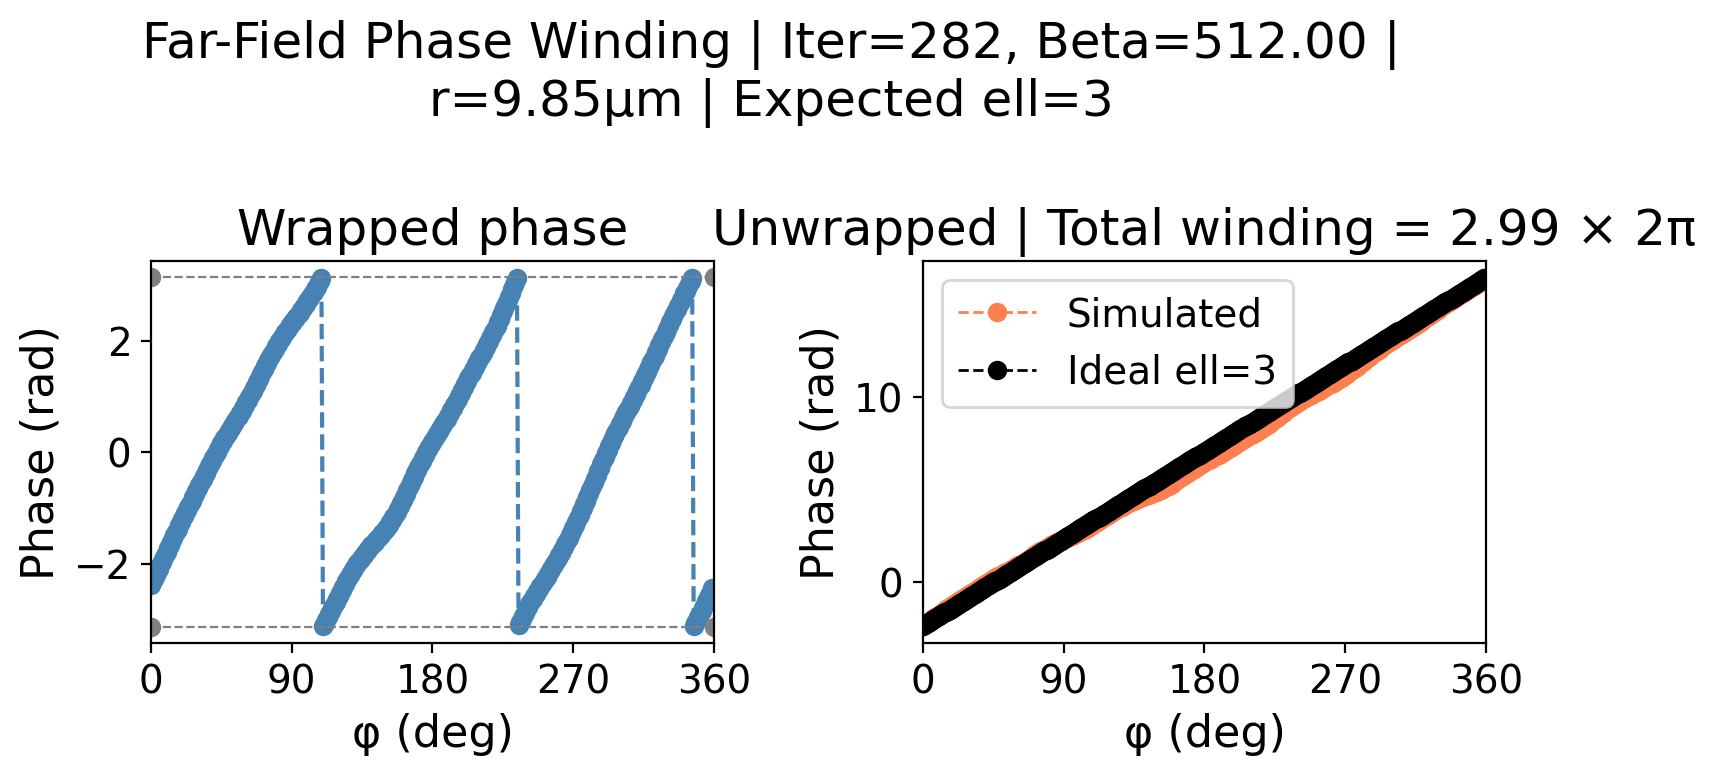
\includegraphics[width=0.47\textwidth]{img/020_ff_winding_iter_282_beta_512.00_rfraction_0.5468.png}
	    \\(c) & (d)\\[6pt]
	    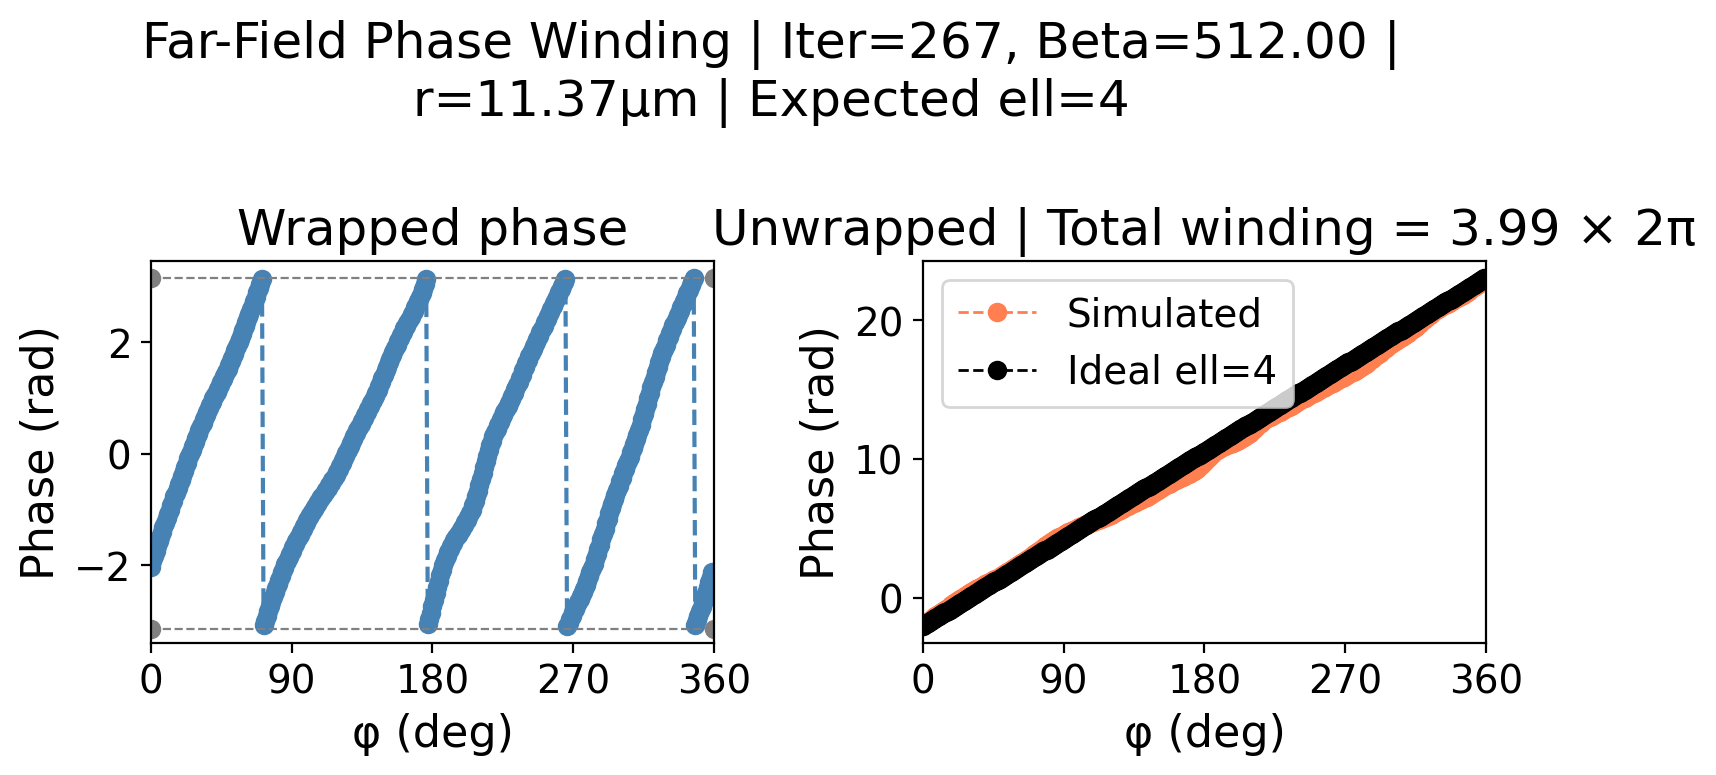
\includegraphics[width=0.47\textwidth]{img/021_ff_winding_iter_267_beta_512.00_rfraction_0.5868.png}&
	    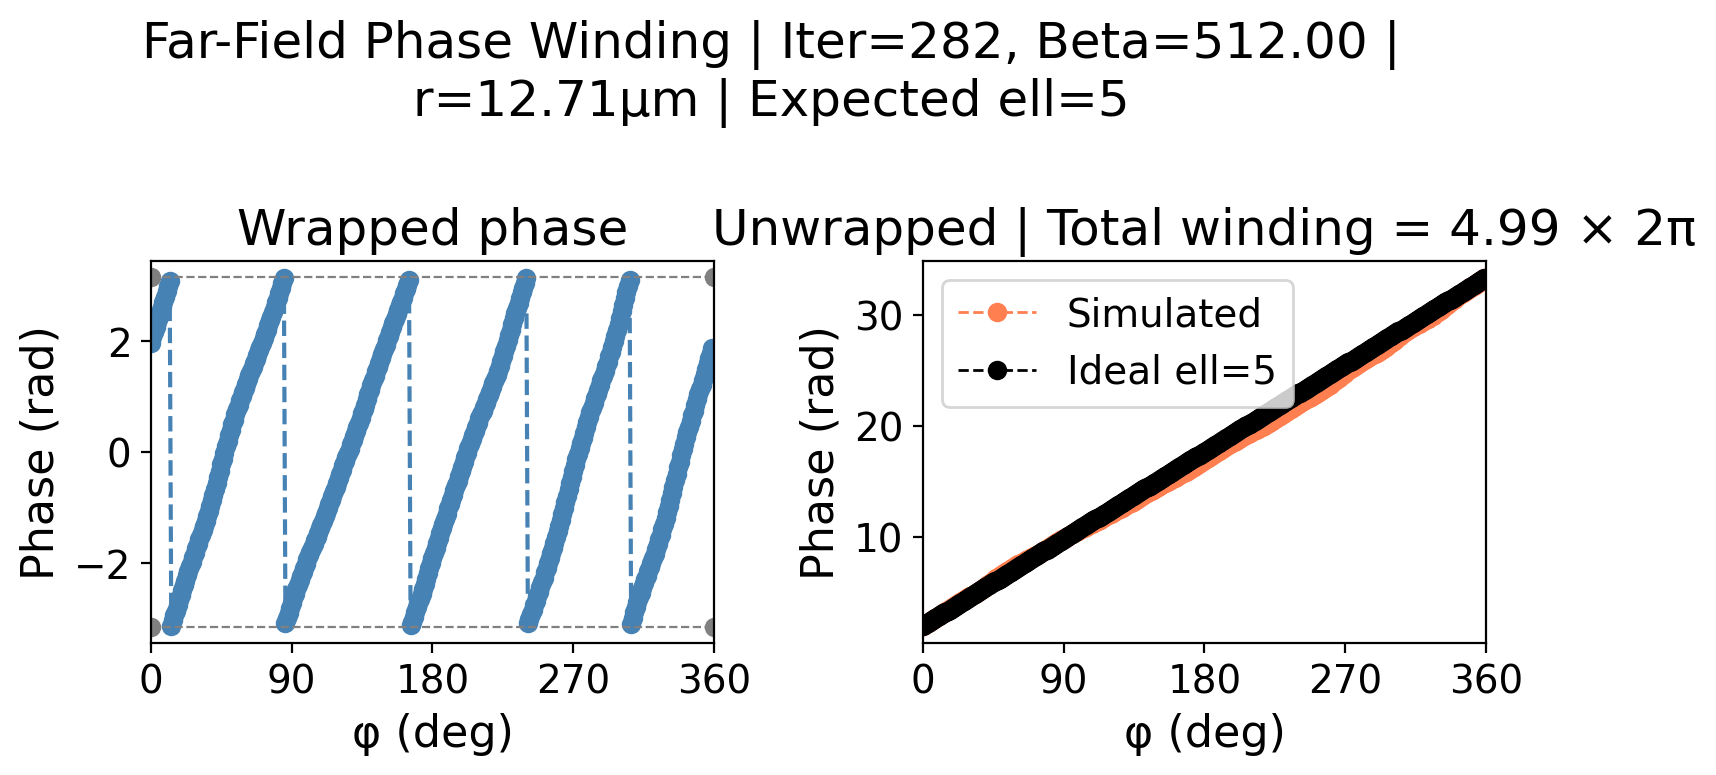
\includegraphics[width=0.47\textwidth]{img/022_ff_winding_iter_282_beta_512.00_rfraction_0.6176.png}
	    \\(e) & (f)
	\end{tabular}
\caption{Far-field phase winding verification: (a)$\sim$(f) $\ell \in \{0, 1, 2, 3, 4, 5\}$, respectively. Sub-panel left column: wrapped phase sampled azimuthally at the peak radius; sub-panel right column: unwrapped phase (orange) compared with the ideal $\ell \times 2\pi$ slope (black dashed line). For all designs, the total unwrapped phase agrees with the target topological charge to within $< 1\%$ error.}
\label{fig:winding_all}
\end{figure}

%===================================================================


\section{Circular Polarization Selectivity}
\label{sec:pol_selectivity}
To confirm whether the optimized nanostructure can accurately distinguish polarization states, a cross-polarization excitation test is performed in this section. In valleytronics applications, the $K$-valley and $K'$-valley excitons in a WS$_2$ monolayer emit LCP and RCP light respectively; therefore, the structure must be able to recognize a specific polarization state while suppressing coupling to the non-target polarization.

All topological structures were topology-optimized using an LCP point source. To quantitatively examine their selectivity, all five non-Gaussian designs ($\ell = 1$ to $5$) were tested: the input source is changed to an RCP point source of opposite handedness, and the far-field OAM mode purity as well as $|\text{Overlap}|^2$ are evaluated for each structure.

The results are summarized in Table~\ref{tab:rcp_selectivity}. In all five cases, the RCP-excited far-field purity of the target mode collapses to near-zero values: $\ell = 1, 3$ give $0.03\%$, while $\ell = 2, 4, 5$ all round to $0.00\%$ (actual values $< 0.005\%$). The $|\text{Overlap}|^2$ values are likewise indistinguishable from zero for all designs. These results stand in sharp contrast to the high-purity LCP-excited performance listed in Table~\ref{tab:results_summary} ($82\%$--$99\%$), directly demonstrating that every LCP-optimized structure exhibits extremely strong circular polarization selectivity.

\begin{table}[htb]
\centering
\caption{RCP cross-polarization excitation test results for $\ell = 1$ to $5$ (far-field plane at $z = 10\,z_R$). Values are rounded to two decimal places; entries showing $0.00$ indicate actual values $< 0.005$.}
\label{tab:rcp_selectivity}
    \begin{tabular}{cccc}
        \hline
        $\ell$ & LCP Purity (\%) & RCP Purity (\%) & Valley Contrast Ratio\\
        \hline
        1 & 98.66 & 0.03 & $\approx 3289:1$\\
        2 & 97.96 & 0.00 & $> 19592:1$\\
        3 & 94.13 & 0.03 & $\approx 3138:1$\\
        4 & 81.94 & 0.00 & $> 16388:1$\\
        5 & 82.62 & 0.00 & $> 16524:1$\\
        \hline
    \end{tabular}
\end{table}

For the representative case of $\ell = 3$ (purity $94.13\%$ vs.\ $0.03\%$), the valley contrast ratio reaches approximately $3138:1$, establishing a clear and directly experimentally benchmarkable inter-valley discrimination baseline. The contrast is even larger for $\ell = 2, 4, 5$, where the RCP purity is below the rounding threshold.

This polarization selectivity arises from the geometric phase and near-field asymmetric scattering within the nanostructure. When the non-target polarization (RCP) is incident, the structure cannot satisfy the geometric phase conditions required for OAM mode shaping, and the vast majority of the energy is scattered into stray fields that cannot effectively couple into the far-field target mode.

Figure~\ref{fig:ff_purity_rcp} shows the far-field results for all five designs under RCP excitation alongside their LCP reference, confirming that no recognizable OAM ring or spiral phase structure is recovered in any case.

\begin{figure}[htb]
\centering
    \begin{tabular}{ccc}
        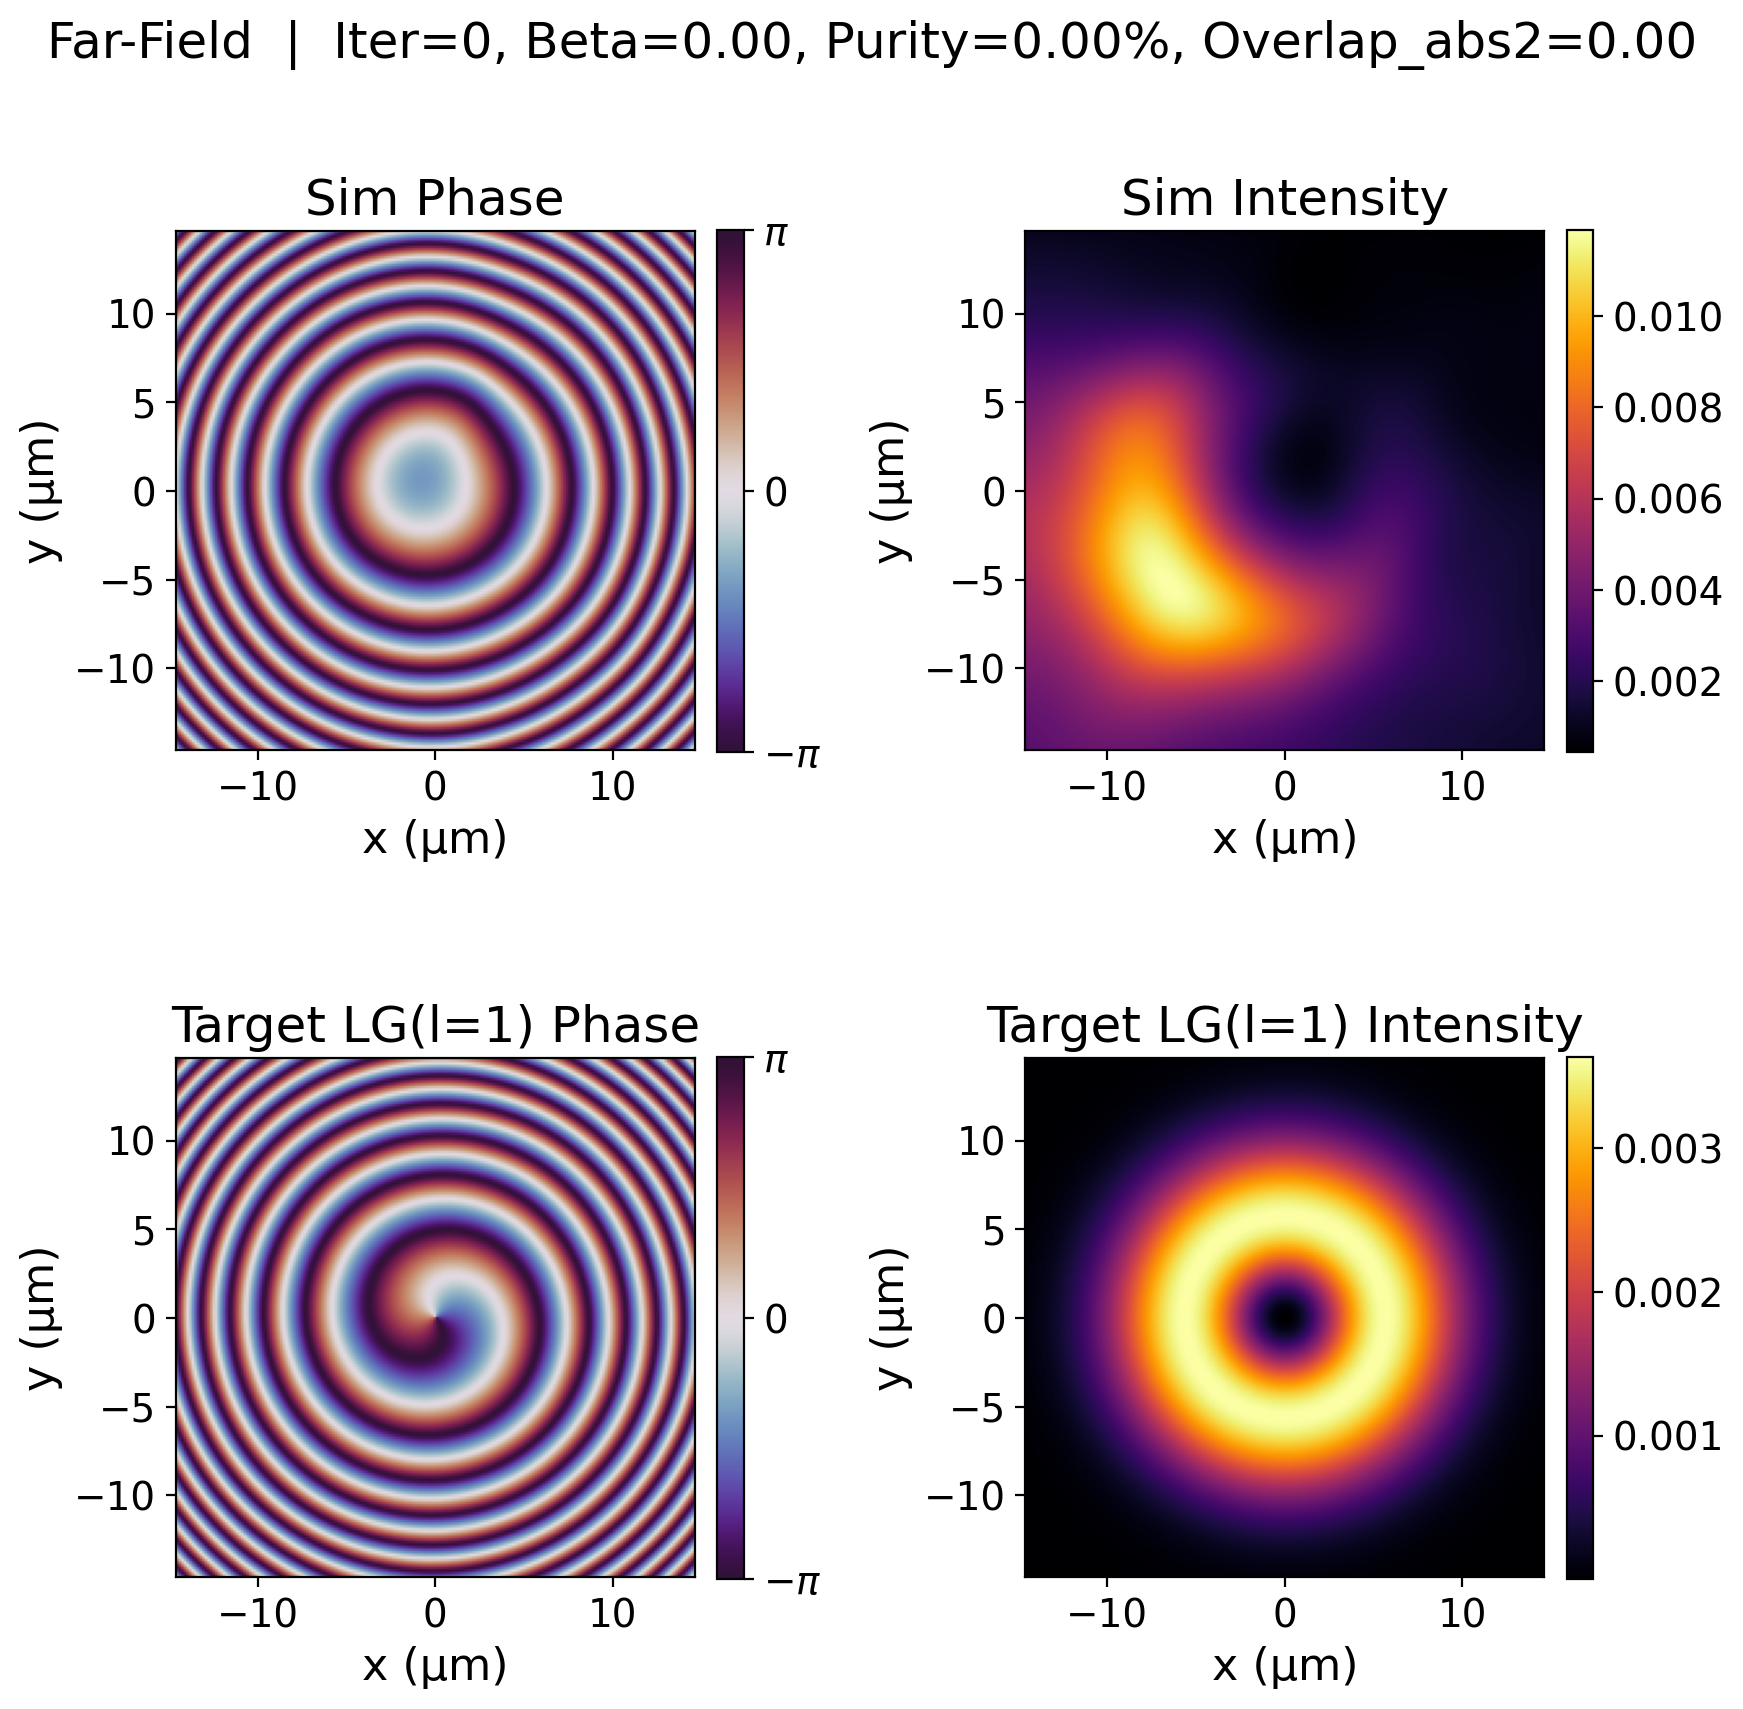
\includegraphics[width=0.30\textwidth,keepaspectratio]{img/018_ff_iter_000_beta_0.00.png} &
        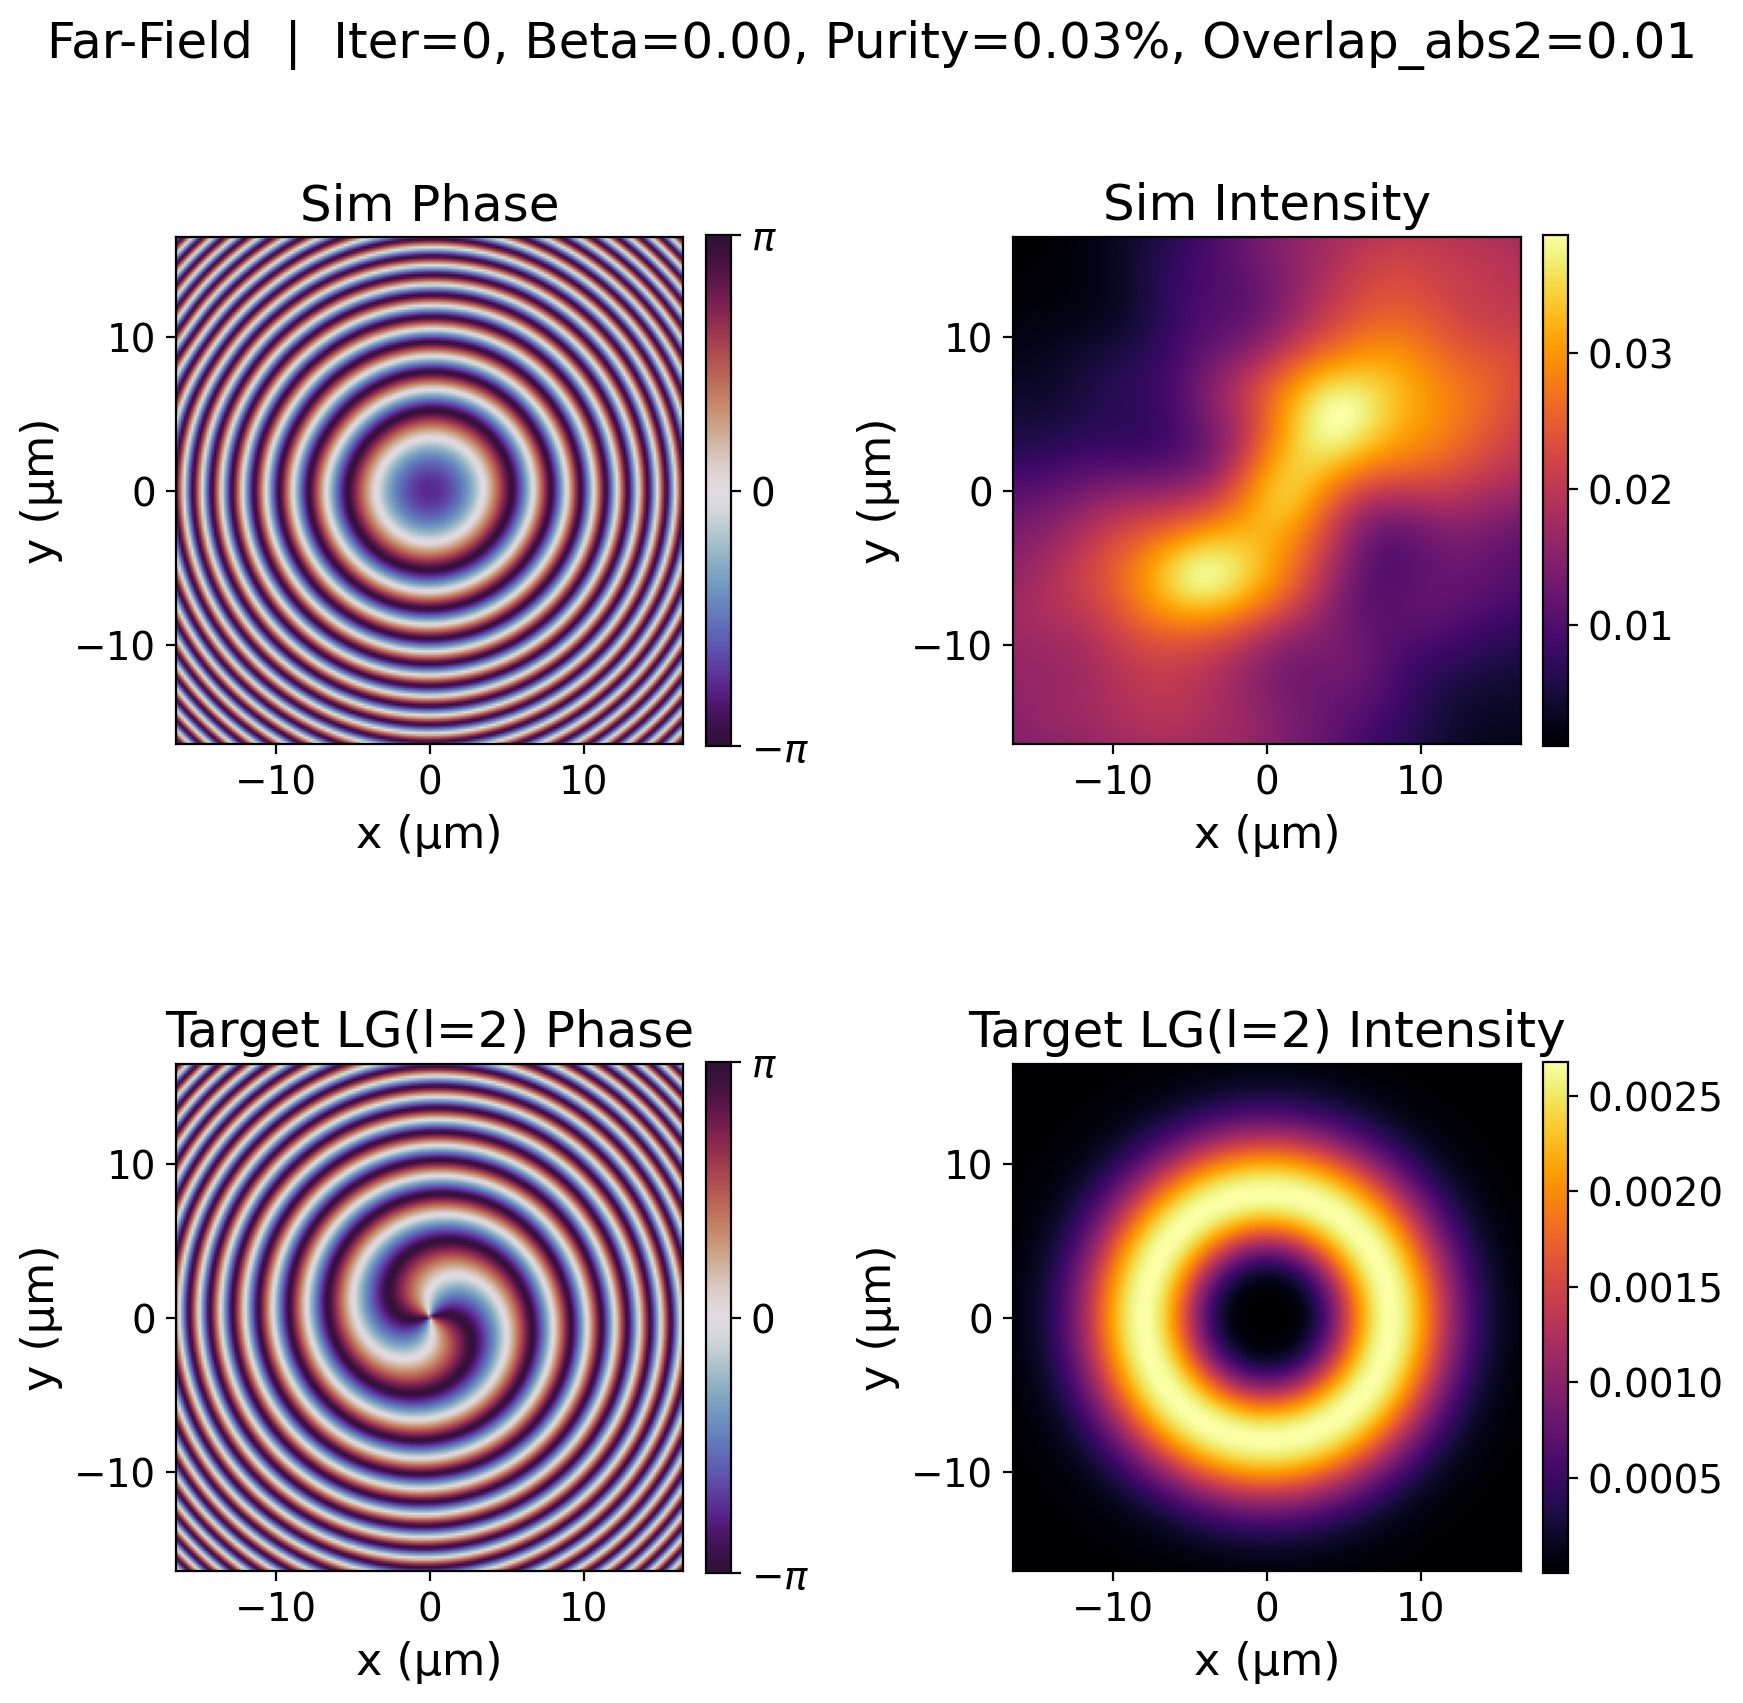
\includegraphics[width=0.30\textwidth,keepaspectratio]{img/013_ff_iter_000_beta_0.00.png} &
        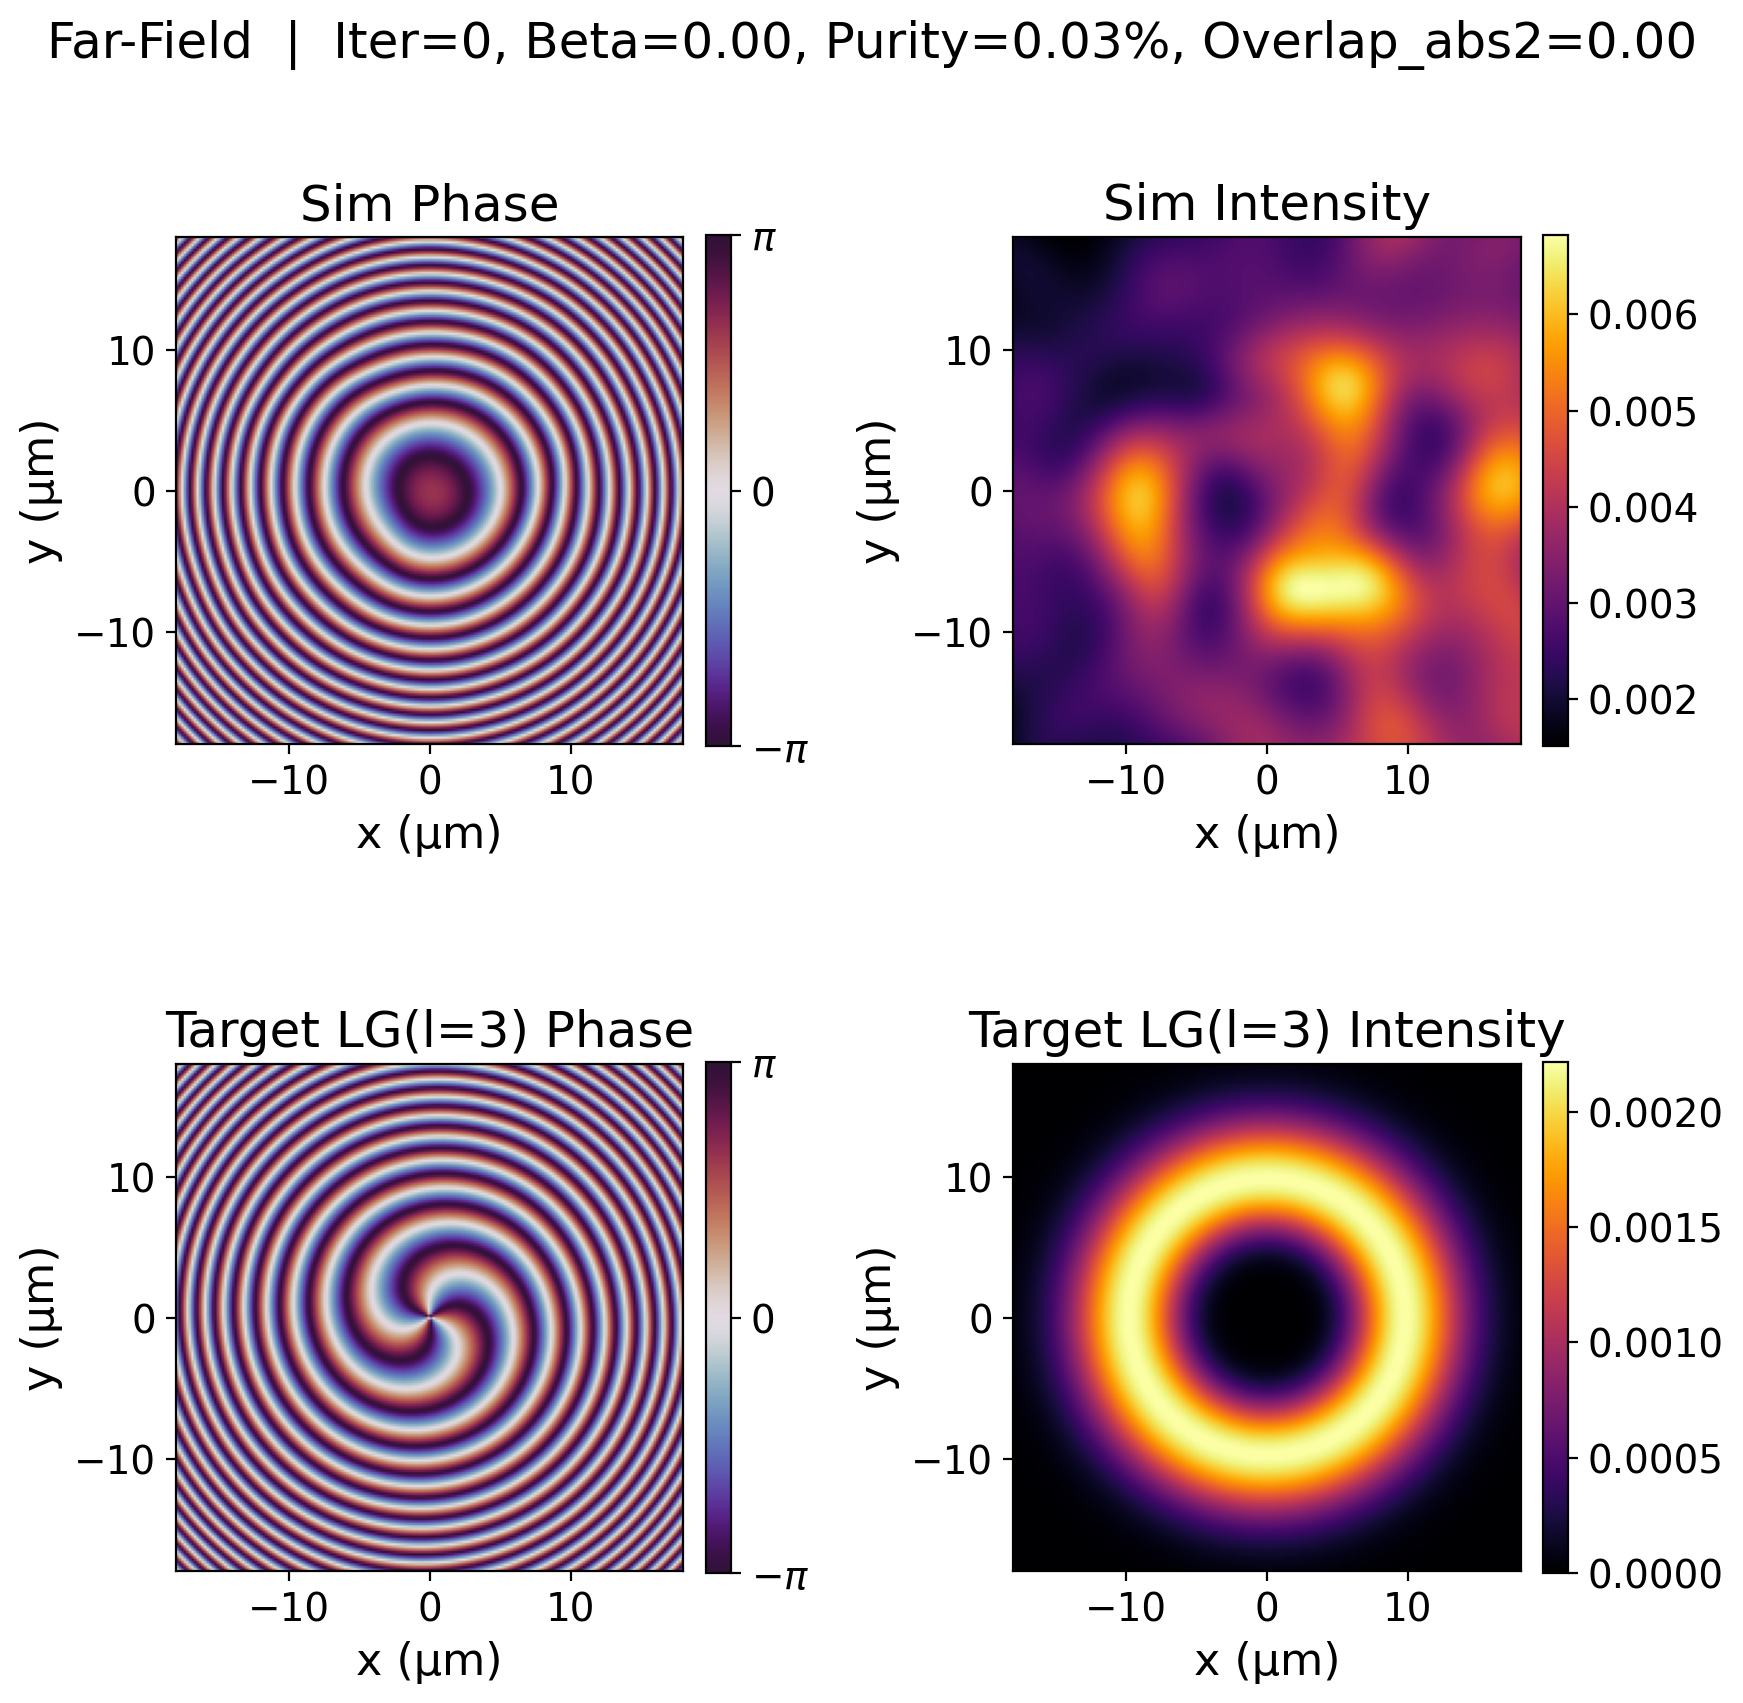
\includegraphics[width=0.30\textwidth,keepaspectratio]{img/rcp.png}
        \\ (a) $\ell=1$, RCP & (b) $\ell=2$, RCP & (c) $\ell=3$, RCP \\[8pt]
        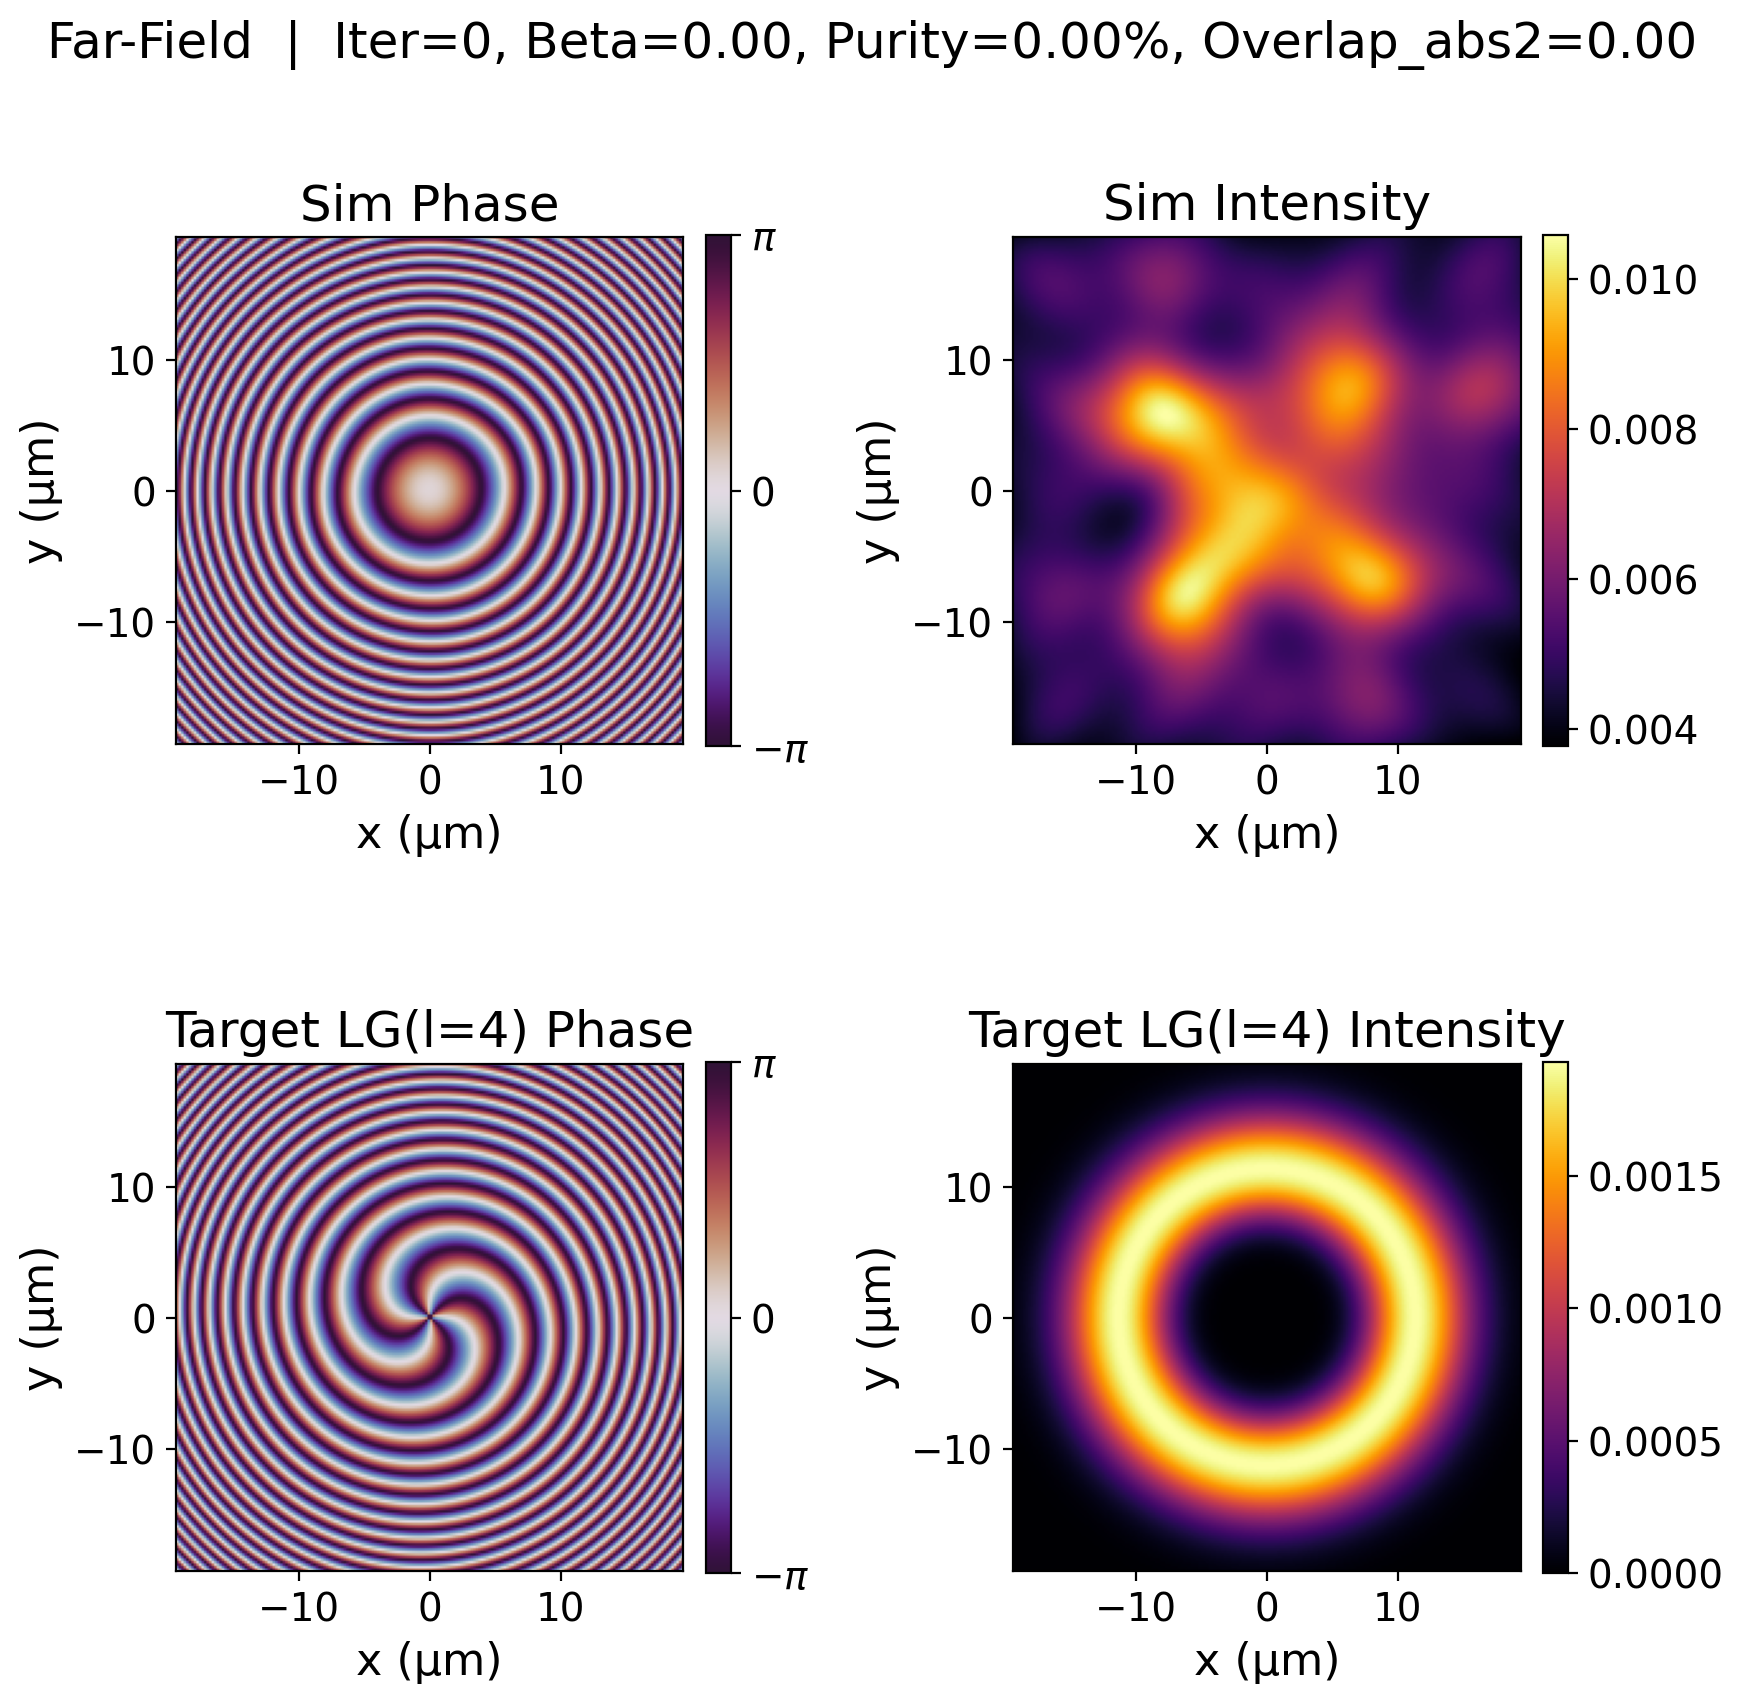
\includegraphics[width=0.30\textwidth,keepaspectratio]{img/021_ff_iter_000_beta_0.00.png} &
        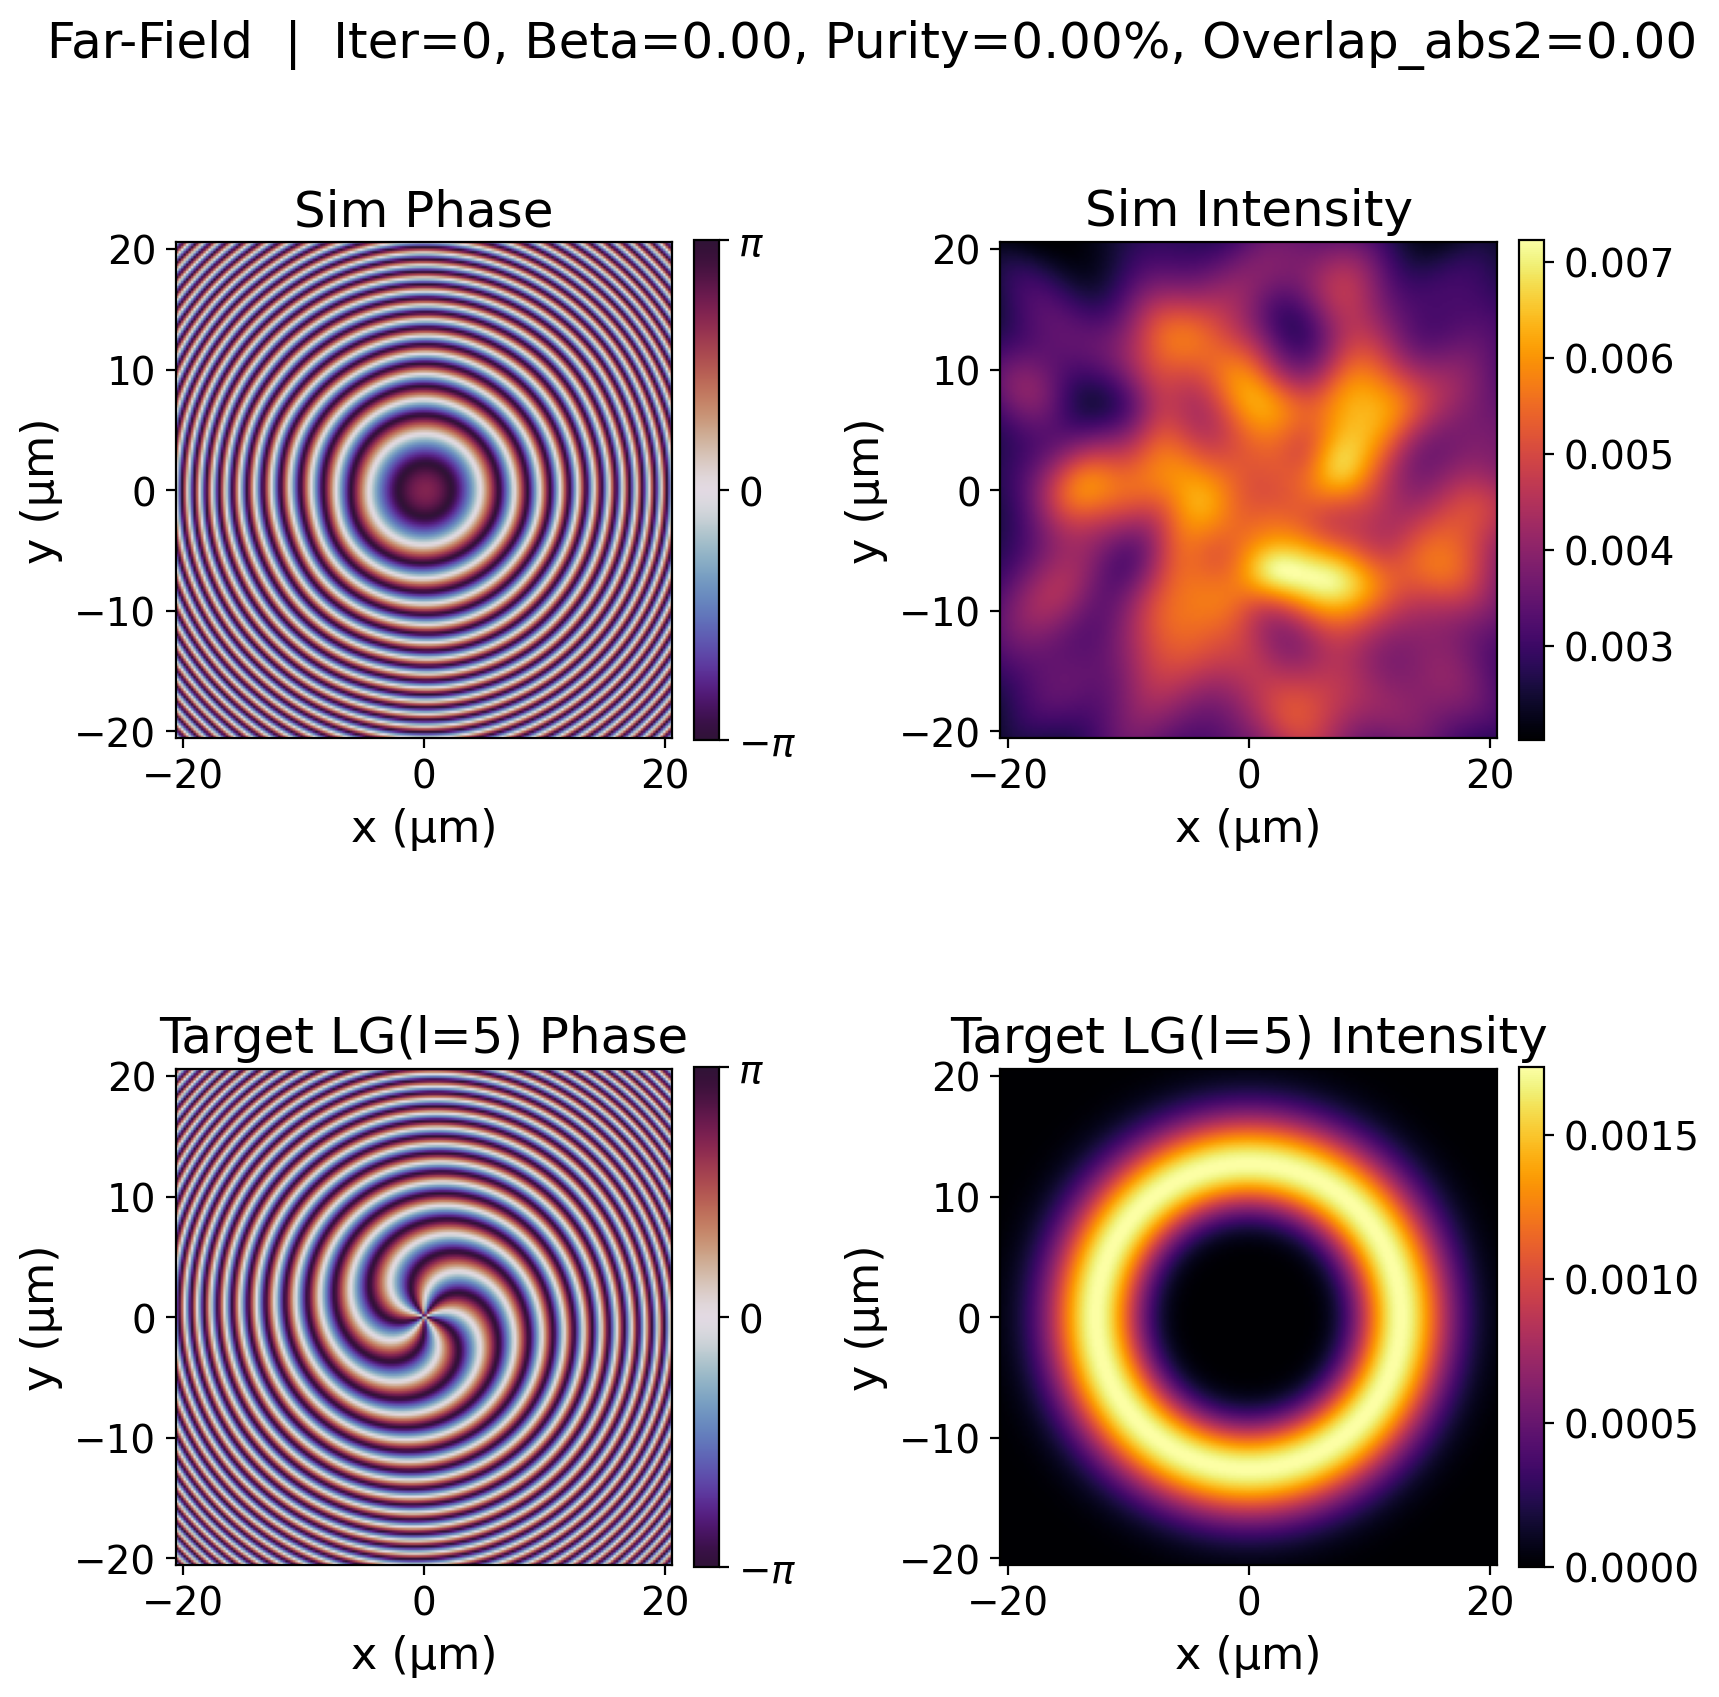
\includegraphics[width=0.30\textwidth,keepaspectratio]{img/022_ff_iter_000_beta_0.00.png} &
        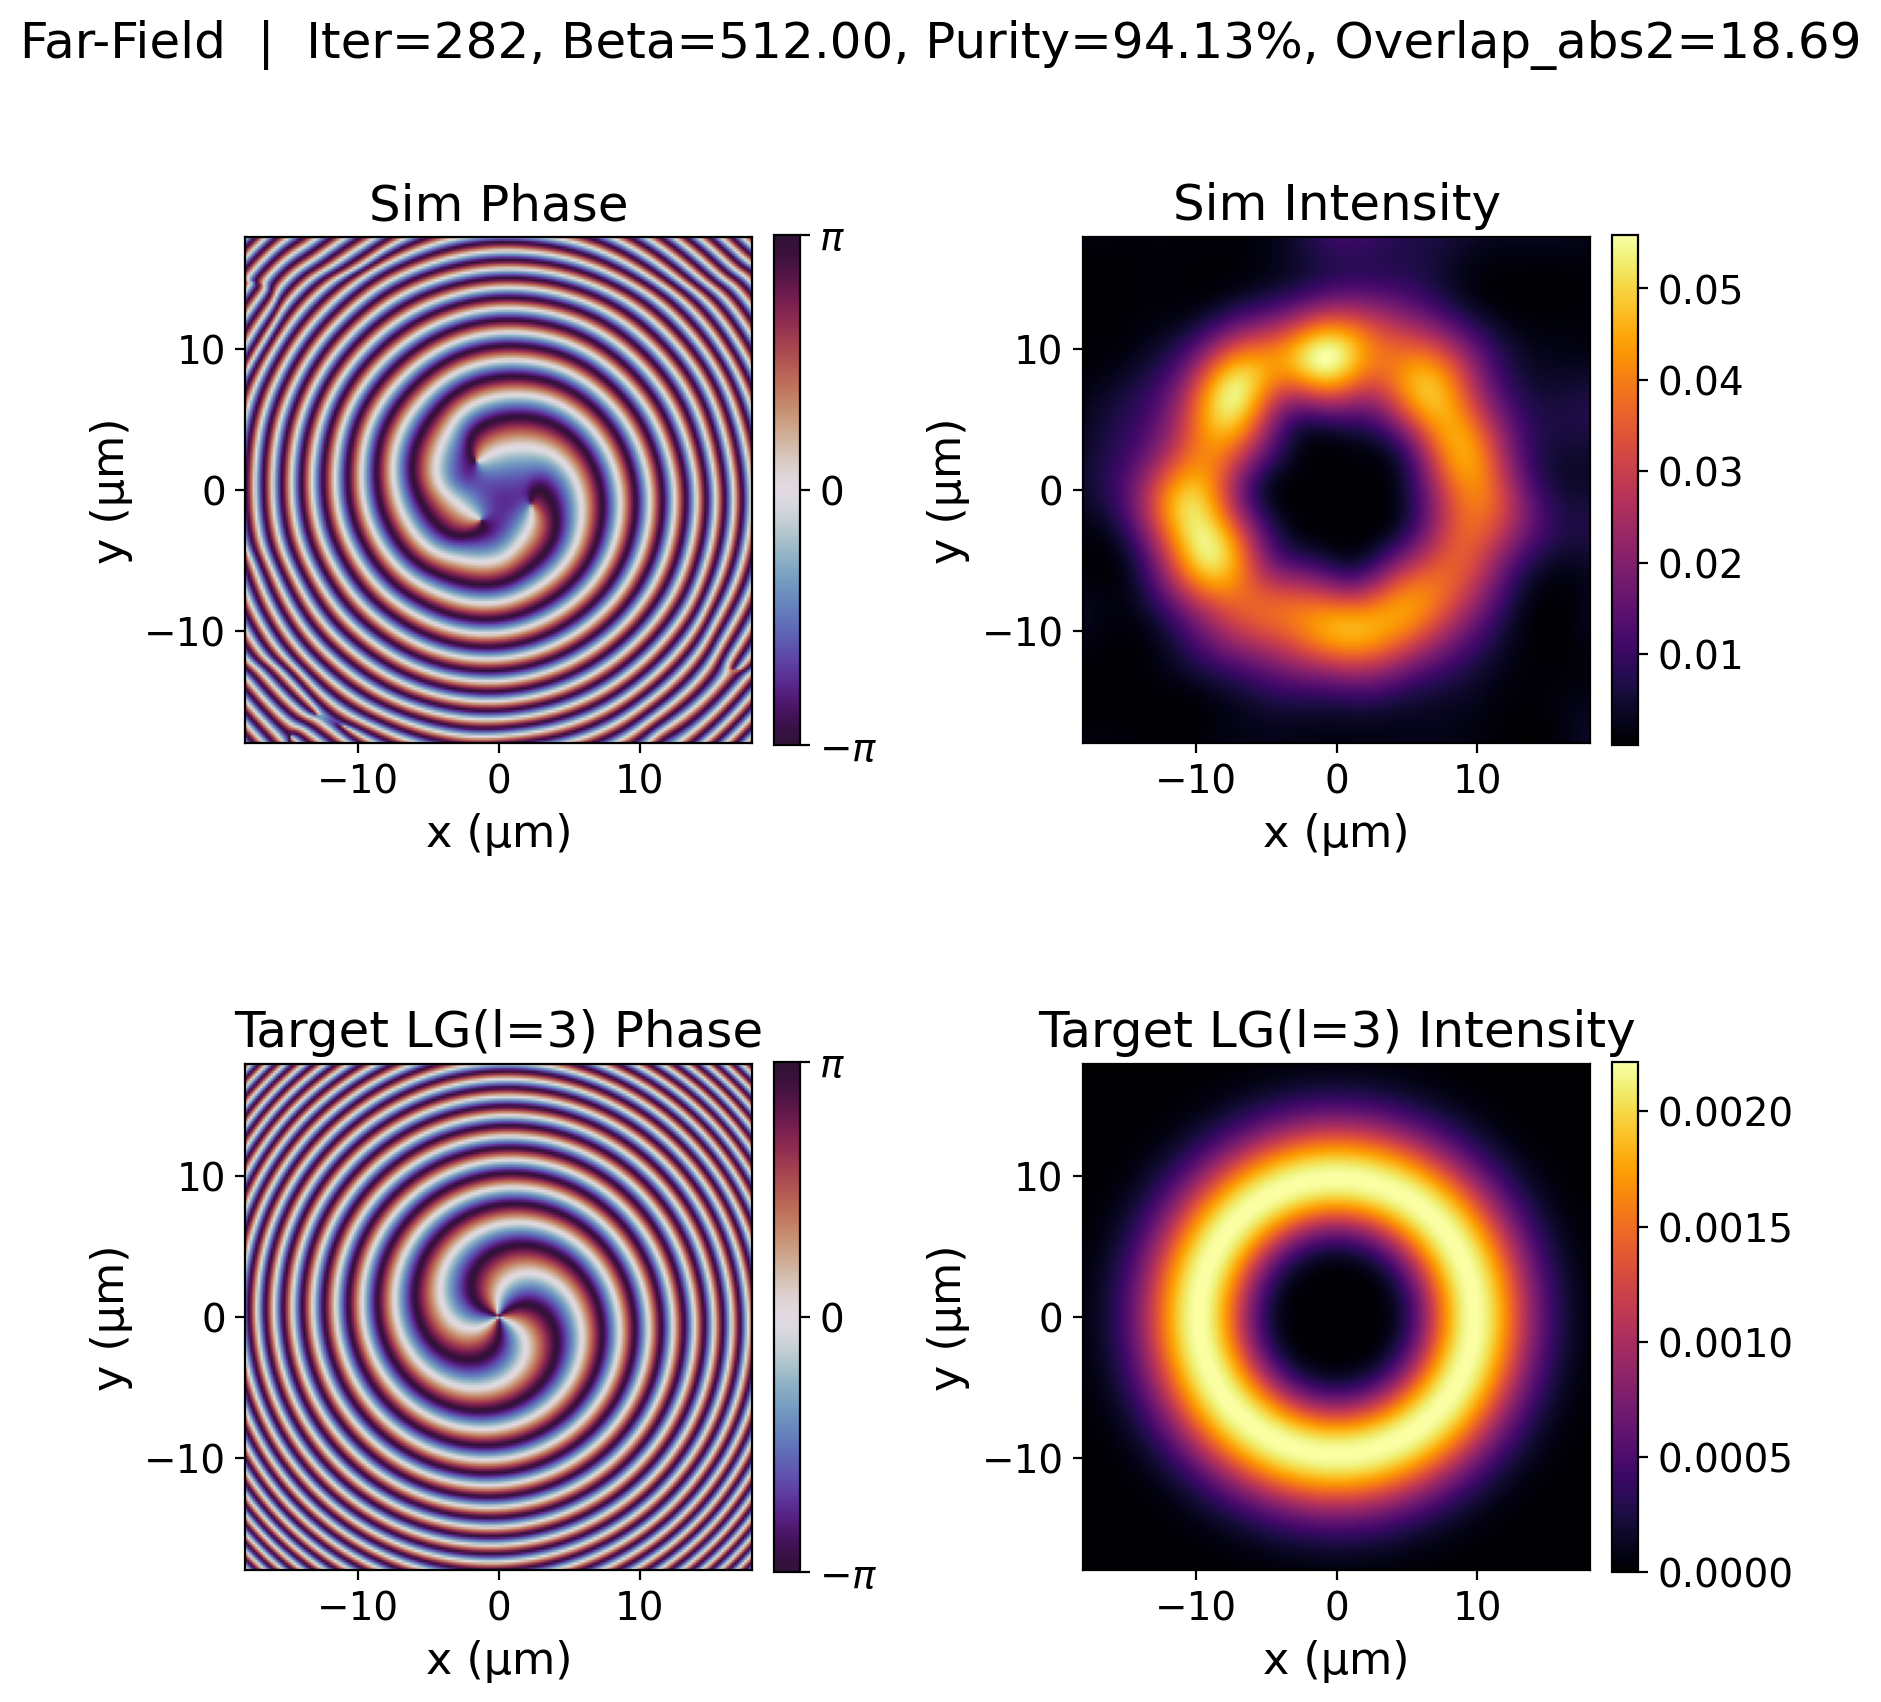
\includegraphics[width=0.30\textwidth,keepaspectratio]{img/020_ff_iter_282_beta_512.00.png}
        \\ (d) $\ell=4$, RCP & (e) $\ell=5$, RCP & (f) $\ell=3$, LCP (reference)
    \end{tabular}
\caption{Far-field OAM mode analysis under RCP cross-polarization excitation for $\ell = 1$ to $5$ ((a)--(e)), with the LCP-excited $\ell = 3$ result shown as a reference (f). Under RCP excitation, the far-field purity of the target LG mode collapses to near-zero in all cases (see Table~\ref{tab:rcp_selectivity}), and neither the characteristic doughnut intensity ring nor the spiral phase pattern is recovered, confirming very strong circular polarization selectivity for all designs.}
\label{fig:ff_purity_rcp}
\end{figure}



%===================================================================


\section{Device Energy Efficiency}
\label{sec:device_efficiency}

Beyond modal purity and phase accuracy, understanding how efficiently the source power is directed upward into the far-field collection cone is essential for assessing the device's practical utility. This section evaluates three complementary efficiency metrics for all six designs and a bare reference case:

\begin{itemize}
    \item $X$ Upward fraction): $X = P_\text{up}/P_\text{total}$, where $P_\text{up}$ is the power collected by a monitor placed above the design layer and $P_\text{total}$ is the total power radiated by the source. This metric directly quantifies the fraction of source energy redirected upward toward the far-field observation side.
    \item $Y$ (Far-field LG purity): The modal purity evaluated at $z = 10\,z_R$ (see Table~\ref{tab:results_summary}).
    \item $Z$ (Device efficiency): $Z = X \times Y$, combining upward extraction and mode quality into a single end-to-end figure of merit.
\end{itemize}

Table~\ref{tab:device_efficiency} summarizes the results for all six designs alongside a pure-air baseline (the same dipole source without any GaP nanostructure, only the diamond substrate). Figure~\ref{fig:monitor_positions} illustrates the power monitor placement.

\begin{table}[htb]
\centering
\caption{Device energy efficiency for all six optimized designs and a pure-air baseline.}
\label{tab:device_efficiency}
\begin{tabular}{cccccc}
\hline
Structure & $P_\text{up}$ (a.u.) & $P_\text{total}$ (a.u.) & $X$ (\%) & $Y$ (\%) & $Z$ (\%) \\
\hline
Pure Air (baseline) & $5.0\times10^{1}$ & $1.0\times10^{3}$ & 5.04  & 100.00 & 5.04  \\
$\ell = 0$ & $1.6\times10^{2}$ & $9.2\times10^{2}$ & 17.67 & 96.81  & 17.11 \\
$\ell = 1$ & $9.2\times10^{1}$ & $9.5\times10^{2}$ &  9.67 & 98.66  &  9.54 \\
$\ell = 2$ & $3.5\times10^{1}$ & $1.2\times10^{3}$ &  2.93 & 97.96  &  2.87 \\
$\ell = 3$ & $6.3\times10^{1}$ & $1.5\times10^{3}$ &  4.22 & 94.13  &  3.97 \\
$\ell = 4$ & $3.5\times10^{1}$ & $1.2\times10^{3}$ &  2.93 & 81.94  &  2.40 \\
$\ell = 5$ & $2.4\times10^{1}$ & $1.1\times10^{3}$ &  2.14 & 82.62  &  1.77 \\
\hline
\end{tabular}
\end{table}

The results reveal a clear performance hierarchy. The $\ell = 0$ design achieves the highest device efficiency of $Z = 17.11\%$, representing a $3.4\times$ improvement over the pure-air baseline ($5.04\%$), confirming that the Gaussian-mode nanostructure is highly effective at redirecting near-isotropic dipole radiation upward. The $\ell = 1$ design follows at $Z = 9.54\%$. Higher-order designs ($\ell \ge 2$) show significantly lower upward fractions ($X \le 4.22\%$), bringing the overall device efficiency below $4\%$ despite their high LG modal purity ($Y \ge 82\%$).

Importantly, the dominant bottleneck is the upward fraction $X$ rather than modal purity $Y$: while $Y \ge 82\%$ for all six designs, $X$ spans a much wider range from $2.14\%$ to $17.67\%$. This indicates that the optimizer successfully shapes the correct LG mode profile, but a large fraction of the emitted power is directed downward into the diamond substrate ($n = 2.40$) or scattered laterally. Improving the upward extraction efficiency---for example by introducing a metal reflector below the diamond substrate (discussed in Section~\ref{sec:future_work})---is therefore the most impactful direction for future efficiency gains.

\begin{figure}[htb]
\centering
	\begin{tabular}{cc} 
		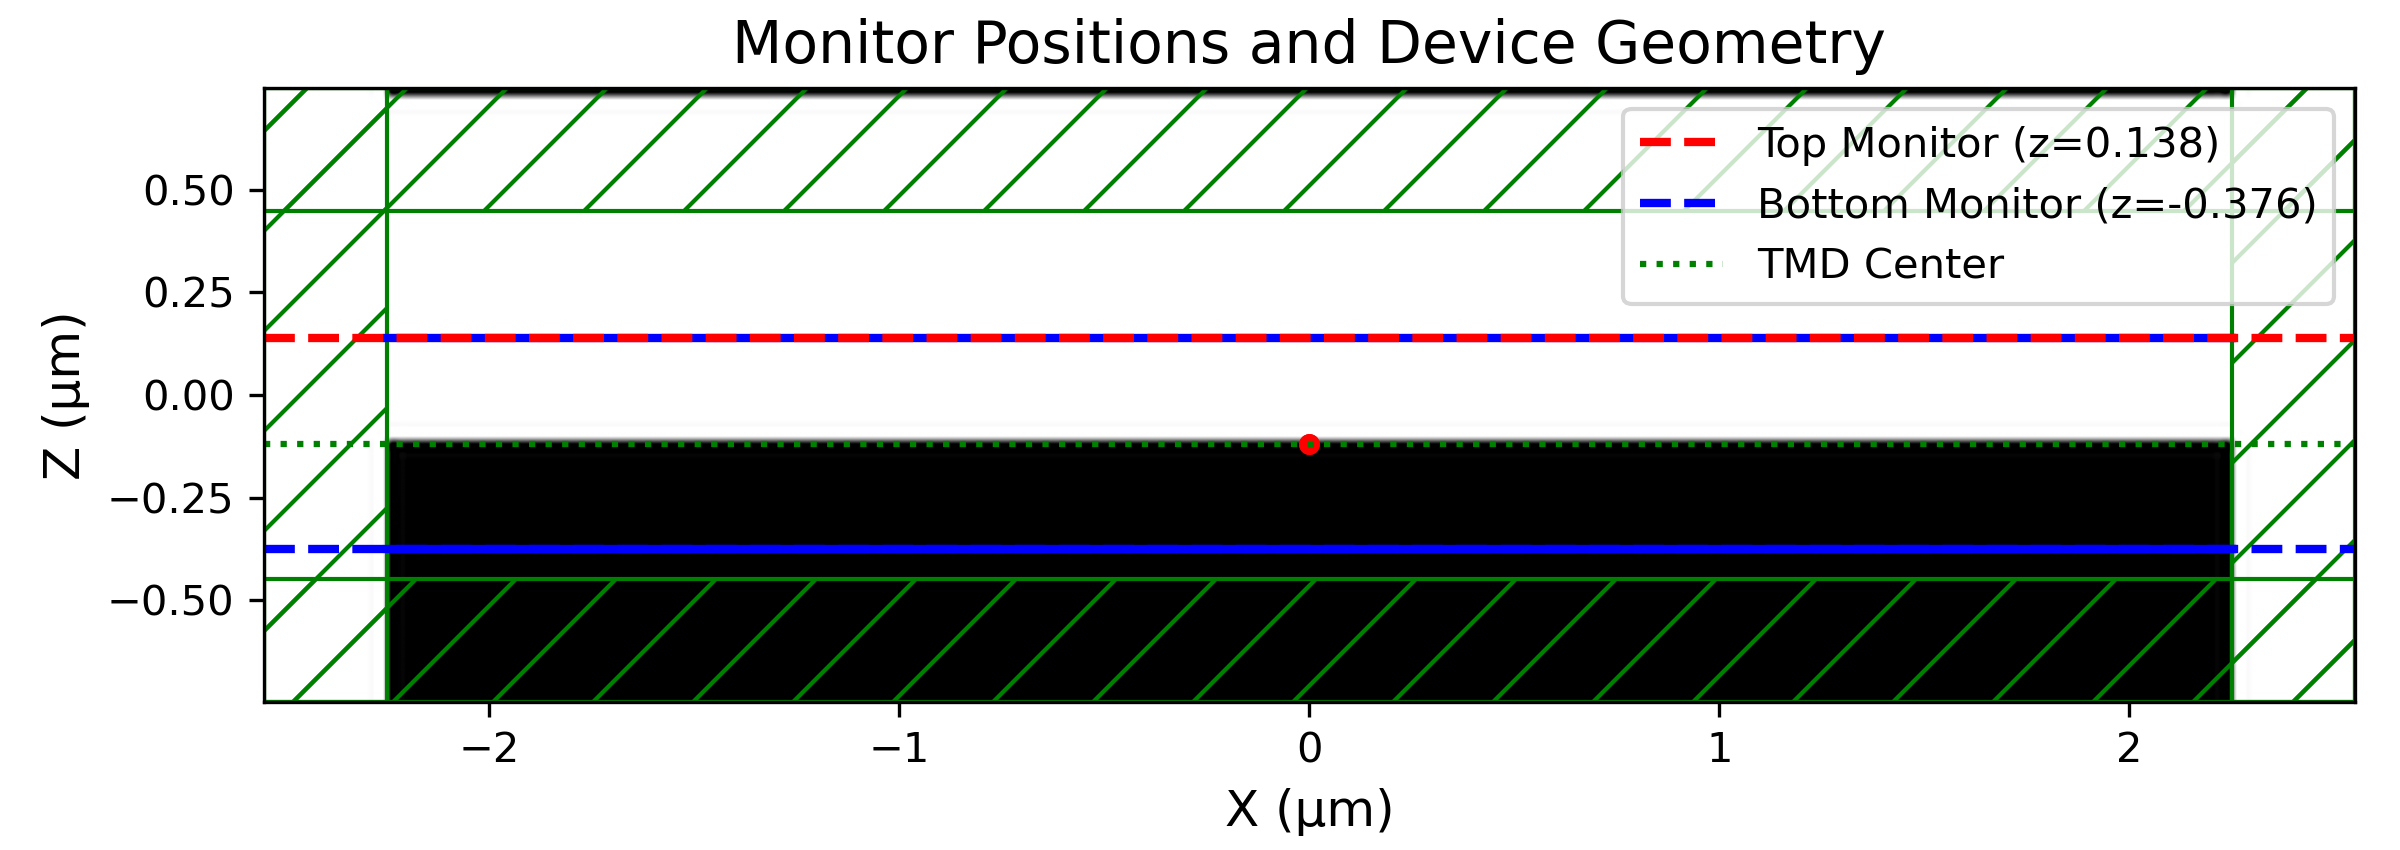
\includegraphics[width=0.48\textwidth]{img/monitor_positions_air.png} & 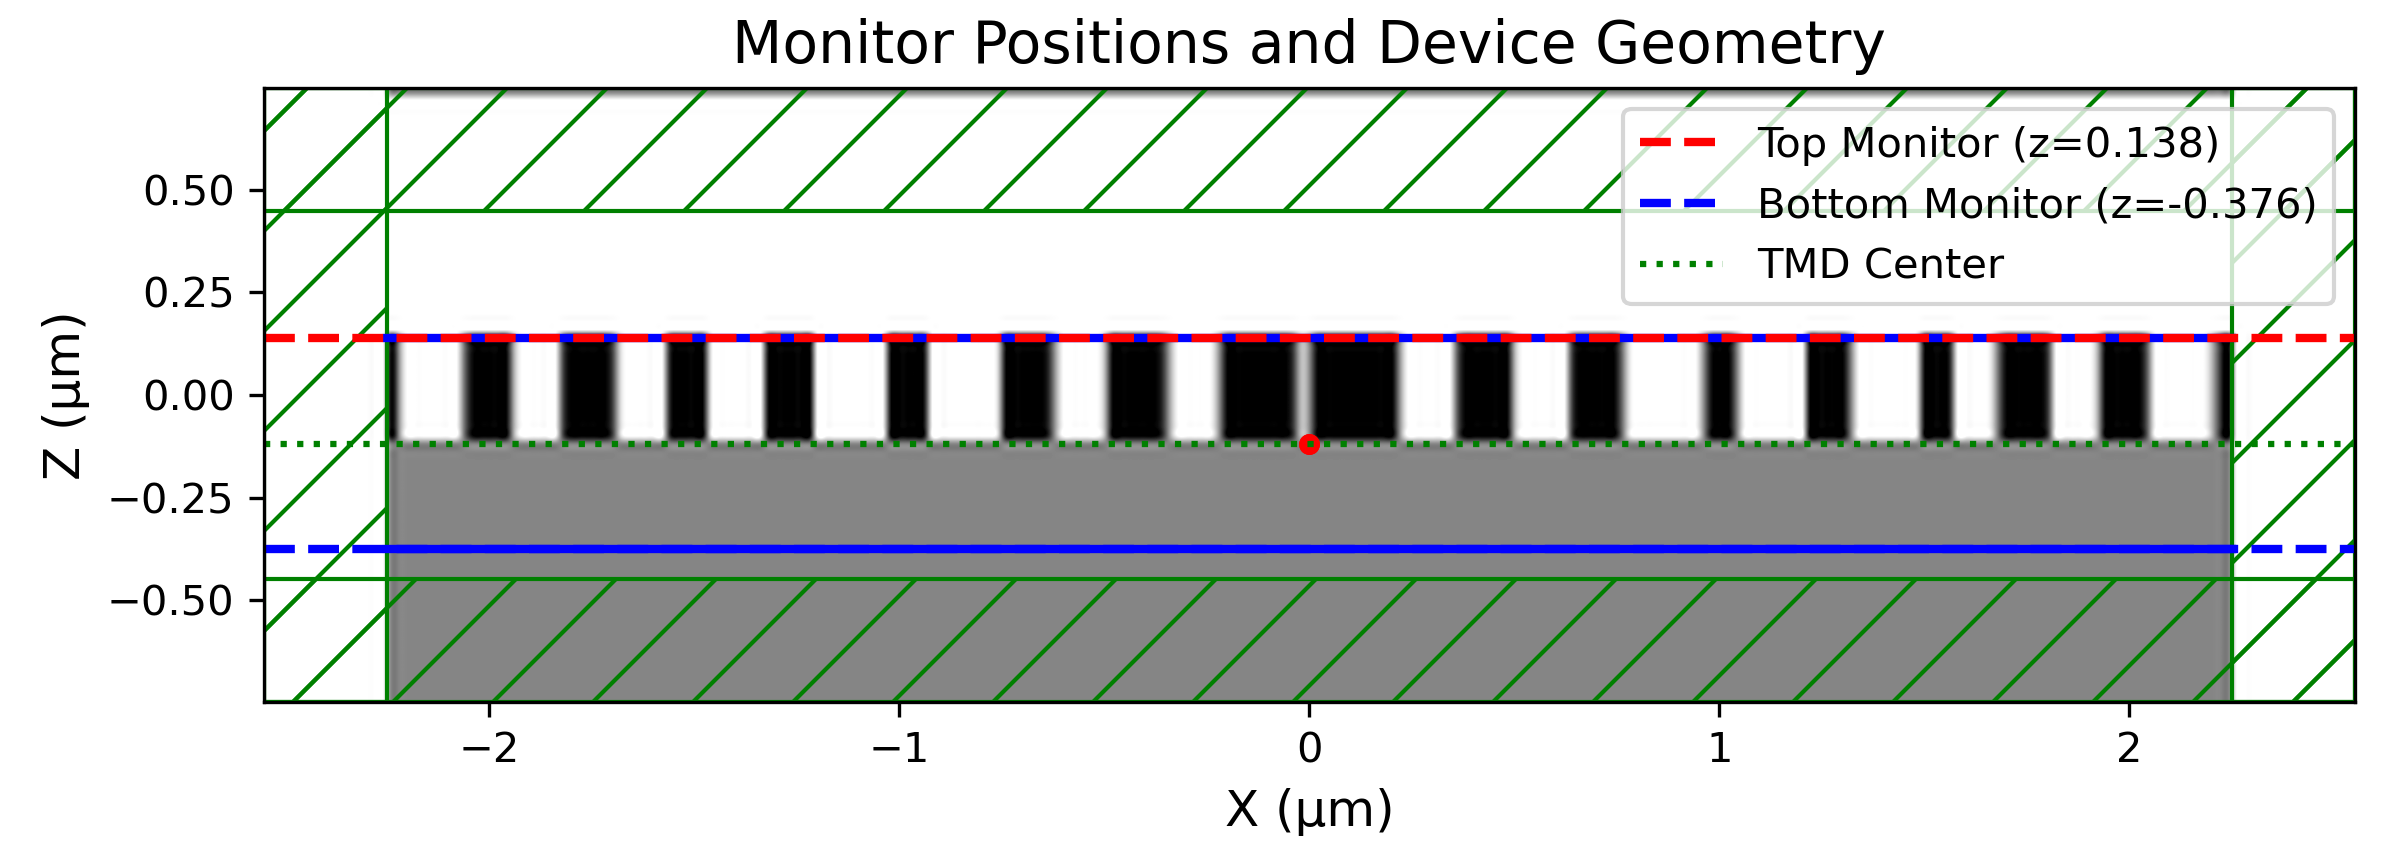
\includegraphics[width=0.48\textwidth]{img/monitor_positions_ell2.png}
		\\(a) Pure-air baseline (no GaP structure) & (b) Representative $\ell = 2$ optimized structure [6pt]
	\end{tabular}
\caption{Power monitor configuration used to evaluate upward extraction efficiency $X$. The upward monitor (red dashed line, above the design layer) captures $P_\text{up}$, while the downward monitor (blue dashed line, below the design layer) captures $P_\text{down}$, with the total power given by $P_\text{total} = P_\text{up} + P_\text{down}$.}
\label{fig:monitor_positions}
\end{figure}